% Options for packages loaded elsewhere
\PassOptionsToPackage{unicode}{hyperref}
\PassOptionsToPackage{hyphens}{url}
%
\documentclass[
  11pt,
]{article}
\usepackage{lmodern}
\usepackage{amssymb,amsmath}
\usepackage{ifxetex,ifluatex}
\ifnum 0\ifxetex 1\fi\ifluatex 1\fi=0 % if pdftex
  \usepackage[T1]{fontenc}
  \usepackage[utf8]{inputenc}
  \usepackage{textcomp} % provide euro and other symbols
\else % if luatex or xetex
  \usepackage{unicode-math}
  \defaultfontfeatures{Scale=MatchLowercase}
  \defaultfontfeatures[\rmfamily]{Ligatures=TeX,Scale=1}
  \setmainfont[]{Helvetica}
\fi
% Use upquote if available, for straight quotes in verbatim environments
\IfFileExists{upquote.sty}{\usepackage{upquote}}{}
\IfFileExists{microtype.sty}{% use microtype if available
  \usepackage[]{microtype}
  \UseMicrotypeSet[protrusion]{basicmath} % disable protrusion for tt fonts
}{}
\makeatletter
\@ifundefined{KOMAClassName}{% if non-KOMA class
  \IfFileExists{parskip.sty}{%
    \usepackage{parskip}
  }{% else
    \setlength{\parindent}{0pt}
    \setlength{\parskip}{6pt plus 2pt minus 1pt}}
}{% if KOMA class
  \KOMAoptions{parskip=half}}
\makeatother
\usepackage{xcolor}
\IfFileExists{xurl.sty}{\usepackage{xurl}}{} % add URL line breaks if available
\IfFileExists{bookmark.sty}{\usepackage{bookmark}}{\usepackage{hyperref}}
\hypersetup{
  hidelinks,
  pdfcreator={LaTeX via pandoc}}
\urlstyle{same} % disable monospaced font for URLs
\usepackage[left=35mm, right=20mm, top=30mm, bottom=30mm]{geometry}
\usepackage{color}
\usepackage{fancyvrb}
\newcommand{\VerbBar}{|}
\newcommand{\VERB}{\Verb[commandchars=\\\{\}]}
\DefineVerbatimEnvironment{Highlighting}{Verbatim}{commandchars=\\\{\}}
% Add ',fontsize=\small' for more characters per line
\usepackage{framed}
\definecolor{shadecolor}{RGB}{248,248,248}
\newenvironment{Shaded}{\begin{snugshade}}{\end{snugshade}}
\newcommand{\AlertTok}[1]{\textcolor[rgb]{0.94,0.16,0.16}{#1}}
\newcommand{\AnnotationTok}[1]{\textcolor[rgb]{0.56,0.35,0.01}{\textbf{\textit{#1}}}}
\newcommand{\AttributeTok}[1]{\textcolor[rgb]{0.77,0.63,0.00}{#1}}
\newcommand{\BaseNTok}[1]{\textcolor[rgb]{0.00,0.00,0.81}{#1}}
\newcommand{\BuiltInTok}[1]{#1}
\newcommand{\CharTok}[1]{\textcolor[rgb]{0.31,0.60,0.02}{#1}}
\newcommand{\CommentTok}[1]{\textcolor[rgb]{0.56,0.35,0.01}{\textit{#1}}}
\newcommand{\CommentVarTok}[1]{\textcolor[rgb]{0.56,0.35,0.01}{\textbf{\textit{#1}}}}
\newcommand{\ConstantTok}[1]{\textcolor[rgb]{0.00,0.00,0.00}{#1}}
\newcommand{\ControlFlowTok}[1]{\textcolor[rgb]{0.13,0.29,0.53}{\textbf{#1}}}
\newcommand{\DataTypeTok}[1]{\textcolor[rgb]{0.13,0.29,0.53}{#1}}
\newcommand{\DecValTok}[1]{\textcolor[rgb]{0.00,0.00,0.81}{#1}}
\newcommand{\DocumentationTok}[1]{\textcolor[rgb]{0.56,0.35,0.01}{\textbf{\textit{#1}}}}
\newcommand{\ErrorTok}[1]{\textcolor[rgb]{0.64,0.00,0.00}{\textbf{#1}}}
\newcommand{\ExtensionTok}[1]{#1}
\newcommand{\FloatTok}[1]{\textcolor[rgb]{0.00,0.00,0.81}{#1}}
\newcommand{\FunctionTok}[1]{\textcolor[rgb]{0.00,0.00,0.00}{#1}}
\newcommand{\ImportTok}[1]{#1}
\newcommand{\InformationTok}[1]{\textcolor[rgb]{0.56,0.35,0.01}{\textbf{\textit{#1}}}}
\newcommand{\KeywordTok}[1]{\textcolor[rgb]{0.13,0.29,0.53}{\textbf{#1}}}
\newcommand{\NormalTok}[1]{#1}
\newcommand{\OperatorTok}[1]{\textcolor[rgb]{0.81,0.36,0.00}{\textbf{#1}}}
\newcommand{\OtherTok}[1]{\textcolor[rgb]{0.56,0.35,0.01}{#1}}
\newcommand{\PreprocessorTok}[1]{\textcolor[rgb]{0.56,0.35,0.01}{\textit{#1}}}
\newcommand{\RegionMarkerTok}[1]{#1}
\newcommand{\SpecialCharTok}[1]{\textcolor[rgb]{0.00,0.00,0.00}{#1}}
\newcommand{\SpecialStringTok}[1]{\textcolor[rgb]{0.31,0.60,0.02}{#1}}
\newcommand{\StringTok}[1]{\textcolor[rgb]{0.31,0.60,0.02}{#1}}
\newcommand{\VariableTok}[1]{\textcolor[rgb]{0.00,0.00,0.00}{#1}}
\newcommand{\VerbatimStringTok}[1]{\textcolor[rgb]{0.31,0.60,0.02}{#1}}
\newcommand{\WarningTok}[1]{\textcolor[rgb]{0.56,0.35,0.01}{\textbf{\textit{#1}}}}
\usepackage{longtable,booktabs}
% Correct order of tables after \paragraph or \subparagraph
\usepackage{etoolbox}
\makeatletter
\patchcmd\longtable{\par}{\if@noskipsec\mbox{}\fi\par}{}{}
\makeatother
% Allow footnotes in longtable head/foot
\IfFileExists{footnotehyper.sty}{\usepackage{footnotehyper}}{\usepackage{footnote}}
\makesavenoteenv{longtable}
\usepackage{graphicx,grffile}
\makeatletter
\def\maxwidth{\ifdim\Gin@nat@width>\linewidth\linewidth\else\Gin@nat@width\fi}
\def\maxheight{\ifdim\Gin@nat@height>\textheight\textheight\else\Gin@nat@height\fi}
\makeatother
% Scale images if necessary, so that they will not overflow the page
% margins by default, and it is still possible to overwrite the defaults
% using explicit options in \includegraphics[width, height, ...]{}
\setkeys{Gin}{width=\maxwidth,height=\maxheight,keepaspectratio}
% Set default figure placement to htbp
\makeatletter
\def\fps@figure{htbp}
\makeatother
\setlength{\emergencystretch}{3em} % prevent overfull lines
\providecommand{\tightlist}{%
  \setlength{\itemsep}{0pt}\setlength{\parskip}{0pt}}
\setcounter{secnumdepth}{-\maxdimen} % remove section numbering
\usepackage{setspace}
\doublespacing
\usepackage{titlesec}
\titlespacing{\section}{0pt}{12pt plus 2pt minus 1pt}{0pt plus 1pt minus 1pt}
\titlespacing{\subsection}{0pt}{12pt plus 2pt minus 1pt}{0pt plus 1pt minus 1pt}
\titlespacing{\subsubsection}{0pt}{12pt plus 2pt minus 1pt}{0pt plus 1pt minus 1pt}
\usepackage{sectsty} \sectionfont{\centering}
\usepackage{sectsty} \subsubsectionfont{\emph}
\usepackage{fancyhdr}
\pagestyle{fancy}
\renewcommand{\headrulewidth}{1.5pt}
\renewcommand{\href}[2]{#2\footnote{\url{#1}}}
\setlength{\headheight}{25.66263pt}
\usepackage{pdflscape}
\newcommand{\blandscape}{\begin{landscape}}
\newcommand{\elandscape}{\end{landscape}}
\usepackage{booktabs}
\usepackage{longtable}
\usepackage{array}
\usepackage{multirow}
\usepackage{wrapfig}
\usepackage{float}
\usepackage{colortbl}
\usepackage{pdflscape}
\usepackage{tabu}
\usepackage{threeparttable}
\usepackage{threeparttablex}
\usepackage[normalem]{ulem}
\usepackage{makecell}
\usepackage{xcolor}

\author{}
\date{\vspace{-2.5em}}

\begin{document}

{
\setcounter{tocdepth}{4}
\tableofcontents
}
\begin{Shaded}
\begin{Highlighting}[]
\CommentTok{##    Clear environment and list required packages:}
      \KeywordTok{rm}\NormalTok{(}\DataTypeTok{list=}\KeywordTok{ls}\NormalTok{())  }
\NormalTok{      packages <-}\StringTok{ }\KeywordTok{c}\NormalTok{(}\StringTok{"tidyverse"}\NormalTok{, }\StringTok{"dplyr"}\NormalTok{, }\StringTok{"captioner"}\NormalTok{, }\StringTok{"tinytex"}\NormalTok{, }\StringTok{"kableExtra"}\NormalTok{, }\StringTok{"formattable"}\NormalTok{, }\StringTok{"readr"}\NormalTok{, }\StringTok{"irr"}\NormalTok{,}
                    \StringTok{"psycho"}\NormalTok{, }\StringTok{"afex"}\NormalTok{, }\StringTok{"emmeans"}\NormalTok{, }\StringTok{"janitor"}\NormalTok{, }\StringTok{"psych"}\NormalTok{, }\StringTok{"rstatix"}\NormalTok{, }\StringTok{"ggpubr"}\NormalTok{, }\StringTok{"ggridges"}\NormalTok{, }\StringTok{"grid"}\NormalTok{,}
                    \StringTok{"gridExtra"}\NormalTok{, }\StringTok{"bibtex"}\NormalTok{, }\StringTok{"apa"}\NormalTok{, }\StringTok{"car"}\NormalTok{)}
\NormalTok{      packages_to_install <-}\StringTok{ }\NormalTok{packages[}\OperatorTok{!}\NormalTok{(packages }\OperatorTok\StringTok{ }\KeywordTok{installed.packages}\NormalTok{()[,}\StringTok{"Package"}\NormalTok{])]}
      \ControlFlowTok{if}\NormalTok{(}\KeywordTok{length}\NormalTok{(packages_to_install)) }\KeywordTok{install.packages}\NormalTok{(packages_to_install)}
      \KeywordTok{invisible}\NormalTok{(}\KeywordTok{suppressPackageStartupMessages}\NormalTok{(}\KeywordTok{lapply}\NormalTok{(packages, library, }\DataTypeTok{character.only =} \OtherTok{TRUE}\NormalTok{)))}
      \CommentTok{#devtools::install_github("crsh/papaja")}
      \KeywordTok{library}\NormalTok{(papaja)}
      \CommentTok{#tinytex::install_tinytex()}
\CommentTok{##    Write references file for all of the packages used, and general R ref:}
      \CommentTok{#write.bib(packages, "resources/packages.bib")}
      \CommentTok{#write.bib(citation(), "resources/base.bib")}
      \KeywordTok{options}\NormalTok{(}\DataTypeTok{scipen=}\DecValTok{999}\NormalTok{)   }\CommentTok{# Turn off scientific notation for numbers printed to the Console. }
\CommentTok{###################################################################################################################}
\CommentTok{##  Define function to get package version: }
\NormalTok{    packages_versions <-}\StringTok{ }\ControlFlowTok{function}\NormalTok{(p) \{}
        \KeywordTok{paste}\NormalTok{(}\KeywordTok{packageDescription}\NormalTok{(p)}\OperatorTok{$}\NormalTok{Package, }\KeywordTok{packageDescription}\NormalTok{(p)}\OperatorTok{$}\NormalTok{Version, }\DataTypeTok{sep =} \StringTok{" "}\NormalTok{)\}    }
\CommentTok{##  Define function used in data tidying:}
\NormalTok{    coalesce_by_column <-}\StringTok{ }\ControlFlowTok{function}\NormalTok{(df) \{}\KeywordTok{return}\NormalTok{(dplyr}\OperatorTok{::}\KeywordTok{coalesce}\NormalTok{(}\OperatorTok{!!!}\StringTok{ }\KeywordTok{as.list}\NormalTok{(df)))\}}
\CommentTok{##  Define function to format t-test results:}
\NormalTok{    ttest.writeup <-}\StringTok{ }\ControlFlowTok{function}\NormalTok{(i)\{}
        \KeywordTok{paste0}\NormalTok{(}\StringTok{"*t*("}\NormalTok{, i}\OperatorTok{$}\NormalTok{df, }\StringTok{") = "}\NormalTok{,}
            \KeywordTok{round}\NormalTok{(i}\OperatorTok{$}\NormalTok{statistic, }\DecValTok{2}\NormalTok{), }\StringTok{", *p* "}\NormalTok{,}
                \KeywordTok{ifelse}\NormalTok{(i}\OperatorTok{$}\NormalTok{p.adj }\OperatorTok{<}\StringTok{ }\FloatTok{.001}\NormalTok{, }\StringTok{"< .001"}\NormalTok{,}
                       \KeywordTok{paste0}\NormalTok{(}\StringTok{"= "}\NormalTok{, }\KeywordTok{round}\NormalTok{(i}\OperatorTok{$}\NormalTok{p.adj, }\DecValTok{2}\NormalTok{))))\}}
    
    
\NormalTok{    independent.ttest.writeup <-}\StringTok{ }\ControlFlowTok{function}\NormalTok{(i)\{}
        \KeywordTok{paste0}\NormalTok{(}\StringTok{"*t*("}\NormalTok{, (i}\OperatorTok{$}\NormalTok{n1 }\OperatorTok{+}\StringTok{ }\NormalTok{i}\OperatorTok{$}\NormalTok{n2) }\OperatorTok{-}\StringTok{ }\DecValTok{2}\NormalTok{, }\StringTok{") = "}\NormalTok{,}
            \KeywordTok{round}\NormalTok{(i}\OperatorTok{$}\NormalTok{statistic, }\DecValTok{2}\NormalTok{), }\StringTok{", *p* "}\NormalTok{,}
                \KeywordTok{ifelse}\NormalTok{(i}\OperatorTok{$}\NormalTok{p.adj }\OperatorTok{<}\StringTok{ }\FloatTok{.001}\NormalTok{, }\StringTok{"< .001"}\NormalTok{,}
                       \KeywordTok{paste0}\NormalTok{(}\StringTok{"= "}\NormalTok{, }\KeywordTok{round}\NormalTok{(i}\OperatorTok{$}\NormalTok{p.adj, }\DecValTok{2}\NormalTok{))))\}}
        
        
\CommentTok{##  Captioner:}
\NormalTok{    figure_numbering <-}\StringTok{ }\KeywordTok{captioner}\NormalTok{()}
\NormalTok{    table_numbering <-}\StringTok{ }\KeywordTok{captioner}\NormalTok{(}\DataTypeTok{prefix =} \StringTok{"Table"}\NormalTok{)}
\NormalTok{    appendix_numbering <-}\StringTok{ }\KeywordTok{captioner}\NormalTok{(}\DataTypeTok{prefix =} \StringTok{"Appendix"}\NormalTok{, }\DataTypeTok{type =} \KeywordTok{c}\NormalTok{(}\StringTok{"C"}\NormalTok{)) }\CommentTok{## Use letters rather than numbers. }
    \KeywordTok{appendix_numbering}\NormalTok{(}\StringTok{"spelling.corrections"}\NormalTok{, }
                       \StringTok{"Manipulations / spelling corrections of naming responses (Experiment 2)."}\NormalTok{, }\DataTypeTok{display =} \OtherTok{FALSE}\NormalTok{)}
    \KeywordTok{appendix_numbering}\NormalTok{(}\StringTok{"exp2.full.norms"}\NormalTok{, }
                       \StringTok{"Normative data for newly curated photograph items (Experiment 2)."}\NormalTok{, }\DataTypeTok{display =} \OtherTok{FALSE}\NormalTok{)}
\end{Highlighting}
\end{Shaded}

\newpage

\hypertarget{chapter-1}{%
\section{Chapter 1}\label{chapter-1}}

\hypertarget{lit-review}{%
\subsection{Lit Review}\label{lit-review}}

Hamilton and Geraci (2006)

IMPLICIT MEMORY: PSE results from conceptual processing of a picture's
distinctive features (rather than semantic information). General
semantic task: ``What is a used car sometimes called?'' No PSE.
Distinctive conceptual information task: ``What fruit is egg shaped?''
PSE.

EXPLICIT RECOGNITION: PSE always evident?

aMCI Show larger PSE effects than controls.

Impaired REC, so this PSE must rely on FAM?

Mixed findings whether fam is intact in aMCI. Intact - generally use
picture stim. Impaired - generally use verbal stim.

Is PSE in aMCI driven by intact FAM for pictures, but impaired FAM for
words? Yes (Embree, Budson, \& Ally, 2012): aMCI - Picture FAM - same as
healthy OAs aMCI - Word FAM - impaired compared to healthy OAs

Ally, McKeever, 2009: Examined early frontal old/new effect (FAM) in
aMCI: Intact for pictures. Impaired for words. BUT, P did not provide
subjective Rec/Fam reports.

Embree, Budson, \& Ally, 2012: Deep encoding (verbal like/dislike
response). Modified Old/New (6-point rating scale): 6. Certain the item
is old - to - 1. Certain the item is new.

Both used the same picture stim - colour photos.

\#\#\#----------------------------------------

\newpage

\hypertarget{chapter-2}{%
\section{Chapter 2}\label{chapter-2}}

\hypertarget{background}{%
\subsection{Background}\label{background}}

Dual-process theories of recognition memory suggest that two independent
processes - recollection and familiarity - are implicated in the
successful recognition of previously encountered material (Paivio, 1971,
1972). Recollection typically refers to the conscious recall of encoded
information, whereby contextual details (usually obtained by mentally
re-experiencing a previous encounter with the stimulus) facilitate
successful recognition. Familiarity, on the other hand, describes the
unsubstantiated \emph{feeling} of having encountered the stimulus
before, and despite the inability to retrieve any associated diagnostic
information, is still able to produce accurate recognition (Schoemaker,
Gauthier, \& Pruessner, 2014). While single-process accounts of
recognition memory have been proposed, with the view that such
experiences can be understood simply as varying levels of memory
strength (Dunn, 2008; Squire, Wixted, \& Clark, 2007), the majority of
memory researchers agree that multiple processes are necessary to
account for a range of dissociable experimental findings (Yonelinas,
2002). Evidence from studies utilising event related potentials (ERPs;
Curran \& Doyle, 2011), functional magnetic resonance imaging (fMRI;
Scalici, Caltagirone, \& Carlesimo, 2017) and comparisons between
healthy and clinical subject groups (e.g.~Mild Cognitive Impairment;
Belleville, Ménard, \& Lepage, 2011) all implicate the existence of two
functionally distinct processes. Despite this consensus, disagreement
persists in the literature regarding the extent to which recollection
and familiarity are independent, and the methods that should be used to
measure them most effectively (Schoemaker et al., 2014; Yonelinas,
2002).

~

Experiments into recognition memory often focus on obtaining separate
estimates of recollection and familiarity using process-estimation
methods (Yonelinas, 2002). The most commonly used process-estimation
method is the Remember/Know (RK) paradigm (Tulving, 1985) - a task
endorsed by a wide body of literature (Gardiner, 2000; Jacoby, 1991;
Jacoby, Yonelinas, \& Jennings, 1997; Yonelinas \& Jacoby, 1995). In a
typical RK procedure, participants are generally tasked with making
`old' vs.~`new' recognition decisions toward a randomised list of items,
many of which were presented during an earlier encoding phase (targets)
amongst novel items with highly similar characteristics (lures). When a
subject recognises an item, and thus selects \emph{Old}, a follow-up
judgement probes how they arrived at this decision (\emph{Remember} or
\emph{Know}). If the subject was able to recognise the item based on
recollection (i.e.~conscious recall of some diagnostic information: ``I
remember seeing this item earlier''), they should classify their
recognition as \emph{Remember}. If the subject arrived at their
recognition decision due to familiarity (i.e.~a feeling of certainty
that the item was studied in the encoding phase, but unable to recall
and details: ``I know I saw this item earlier, but cannot determine
why''), they should classify their recognition as \emph{Know}. In
addition to the literature endorsing the task in healthy samples, a
large body of research also reports that the RK procedure produces
reliable estimations of recollection and familiarity in clinical
populations (Lombardi, Perri, Fadda, Caltagirone, \& Carlesimo, 2016);
for example, those with Mild Cognitive Impairment (MCI) typically
produce results to suggest recollection impairments but intact
familiarity compared to healthy older adults (Belleville et al., 2011;
Hudon, Belleville, \& Gauthier, 2009; Lombardi et al., 2016; Serra et
al., 2010; Wang et al., 2013).

~

The RK procedure has been modified in a number of ways since its
conception, and continues to adapt as understandings of recollection and
familiarity processes evolve. An early development was the
``independence correction'' - a formula devised to `correct' the
inherent underestimation of familiarity processes within the mutually
exclusive paradigm (Yonelinas \& Jacoby, 1995). Participants are
generally only instructed to select \emph{Know} (a reflection of
familiarity) when there is an absence of recollection, however, this
approach does not allow for the possibility of recollection and
familiarity co-occurring. Proportions of \emph{Know} responses will
likely always be lower than \emph{Remember} if subjects do indeed
perceive to experience both processes simultaneously, since the presence
of recollection necessitates that they select the \emph{Remember} option
among the two choices. When the Yonelinas \& Jacoby (1995) independence
correction is applied, estimates of familiarity are determined by also
taking into account the number of times \emph{Remember} was selected
when calculating the proportion of \emph{Know} responses (Schoemaker et
al., 2014). An alternative to this correction is to modify the response
options available to subjects, so they are able to individually
determine the relative contributions of each process. Higham \& Vokey
(2004) proposed an independent ratings methodology whereby, instead of
the binary \emph{Remember}/\emph{Know} options, subjects are provided
with one rating scale to report the contribution of recollection and
another to report the contribution of familiarity (RF-Ratings).
Participants rate their recognition experience for each process
accordingly: 1 = \emph{definitely no}, 2 = \emph{probably no}, 3 =
\emph{probably yes}, 4 = \emph{definitely yes}. Such options allow for
great variability in the way participants are able to respond, and for
the possibility of both processes occurring conjointly: i) Recollection
without Familiarity (high rating on R, low rating on F); ii) Familiarity
without Recollection (high rating on F, low rating on R); iii) both
Recollection \emph{and} Familiarity (high rating on R and F); iv)
neither R or F, i.e.~a guess (\emph{1} rating on R and F). The
methodology of Higham \& Vokey (2004) has been used in numerous studies
(Brown \& Bodner, 2011; Kurilla \& Westerman, 2008; Tousignant \&
Bodner, 2012), however, it could be argued that this rating task is
somewhat removed from the original \emph{judgement} task, and the extent
to which the increased task complexity affects reports of recognition is
unknown (Tousignant, Bodner, \& Arnold, 2015).

~

Further modifications retain the original two binary response options,
but avoid the mutual exclusivity issue by simply including a \emph{Both}
option (Tousignant et al., 2015). When calculating proportions of
recollection and familiarity, the total proportion of \emph{Both}
responses can then be separately added to the totals for each process.
Recent adaptations of the RK paradigm have also begun to include a
\emph{Guess} response option, allowing participants to report
uncertainty in their recognition decision (Belleville et al., 2011;
Eldridge, Sarfatti, \& Knowlton, 2002; Larsson, Öberg, \& Bäckman, 2006;
Tunney \& Fernie, 2007; Williams, 2019). Previous studies have found
that subjects may falsely assign guesses to the \emph{Know} option when
there is no explicit \emph{Guess} option available (Gardiner, Java, \&
Richardson-Klavehn, 1996; Gardiner \& Ramponi, 1998; Gardiner, Ramponi,
\& Richardson-Klavehn, 2002), on the assumption that this option more
closely resembles their state of low confidence (Tunney \& Fernie,
2007). Responding in this manner may artificially inflate obtained
estimates of familiarity (Tunney \& Fernie, 2007). By including
\emph{Guess}, the likelihood of obtaining false \emph{Know} responses
(i.e.~those that do not reflect underlying familiarity processes) is
reduced (Migo, Mayes, \& Montaldi, 2012).

~

Despite its widespread use, the RK procedure has been criticized for its
reliance on participants' subjective understanding of the provided
instructions (Schoemaker et al., 2014), and the introspective nature of
recognition judgements make it difficult to confirm whether all
participants have understood the definitions (and thus responded)
similarly (Lombardi et al., 2016). It is also difficult to determine
whether subjects interpret the \emph{Remember} and \emph{Know} labels in
the same way that researchers intend (Umanath \& Coane, 2020),
especially as there is evidence to suggest participants struggle to
understand the distinction between the terms (Geraci, McCabe, \&
Guillory, 2009; Rubin \& Umanath, 2015; Williams \& Moulin, 2014).
Williams (2019) assessed the ways in which non-recollective subjective
experiences were defined to participants, and found a great deal of
inconsistency across a range of RK experiments. Some studies even
changed the \emph{Remember} and \emph{Know} labels altogether; many
exchanged the \emph{Know} label with \emph{Familiar} in an effort to
reduce subjects defaulting to colloquial understandings of the word
``know'' which typically indicate high certainty; e.g.~``I \textbf{know}
I saw this item in the study phase'' (Bastin, Van der Linden, Michel, \&
Friedman, 2004; Dobbins, KroU, \& Liu, 1998; Donaldson, Mackenzie, \&
Underhill, 1996; Ingram, Mickes, \& Wixted, 2012). Others also
substitute \emph{Remember} for \emph{Recollection} (Harlow, MacKenzie,
\& Donaldson, 2010). Labels that accurately match the processes they
intend to measure - \emph{Recollection} and \emph{Familiarity} - have
been proposed in an effort to reduce the potentially misleading effects
of the more colloquial \emph{Remember} and \emph{Know}, and thus make it
easier for participants to `map on' the definitions provided by
researchers (Harlow et al., 2010; Mayes, Montaldi, \& Migo, 2007).

~

In addition to the availability of different response options, and the
labels used to describe the underlying processes, there is evidence to
suggest that the format of to-be-remembered stimuli also plays a role in
obtained estimates of recollection and familiarity. The Picture
Superiority Effect (PSE) refers to a robust phenomenon whereby stimuli
presented as pictures are markedly better remembered on tests of recall
or recognition than stimuli presented as words (Shepard, 1967). There is
general agreement that, in recognition memory paradigms, picture
superiority manifests as enhanced recollection rather than familiarity
(Curran \& Doyle, 2011; Rajaram, 1996a). Word stimuli, on the other
hand, appear to produce increased familiarity ratings at test (Ally \&
Budson, 2007). Understanding this phenomenon could help to conceptualise
how memory breaks down in healthy ageing, and in the earliest stages of
amnestic Mild Cognitive Impairment (aMCI). For example, Ally et al.
(2008) demonstrated that, despite similar levels of overall performance
on a recognition task, healthy older adults showed greater picture
superiority effects than younger adults. The memorial benefit of
pictures was indeed evident in both the young and older groups, but the
magnitude of this effect was greater in older adults, who only showed
worse performance when responding to word stimuli. Interestingly,
picture superiority also allows those with aMCI to show performance that
is comparable to healthy older adult controls; despite exhibiting
impaired performance overall, those with aMCI often show intact
familiarity processes when pictures are utilised in recognition memory
paradigms (and impaired familiarity when word stimuli are utilised;
Embree, Budson, \& Ally (2012); Ally et al. (2009a); Ally et al.
(2009b); Wolk, Signoff, \& DeKosky (2008); Algarabel et al. (2009);
Anderson et al. (2008); Hudon et al. (2009); O'Connor \& Ally (2010);
Serra et al. (2010); Westerberg et al. (2006){]}.

~

The objective of the current programme of research is to better
understand how different methodologies inform understandings about the
underlying processes of recollection and familiarity. Across a number of
experiments, the distinctiveness of to-be-remembered stimuli will be
systematically examined to determine the level at which successful
recognition is impacted, and which process(es) are most susceptible. The
aim of the first experiment, outlined below, is to establish baseline
PSE response patterns in a novel, modified RK paradigm. In a 2x3 mixed
factorial design, a within-subjects variable of stimulus type (words /
simple pictures) will be used to determine whether the magnitude of
picture superiority effects (PSEs) is mediated by the particular
response options available at test (between-subjects variable of
response option: RFG, RFBG, RF-Ratings). In each condition, the labels
\emph{Recollection}/\emph{Familiarity} will be used in place of the
standard \emph{Remember}/\emph{Know}, in an effort to reduce the impact
of colloquial understandings on the current experimental definitions. To
avoid guesses biasing estimations of familiarity (Belleville et al.,
2011; Eldridge et al., 2002; Larsson et al., 2006; Tunney \& Fernie,
2007; Williams, 2019), participants in all response-option conditions
are also given the option to report that they are merely \emph{Guessing}
that an item is old. At test, subjects will be presented with either i)
three response options (RFG); ii) four response options (RFBG; where a
\emph{Both} response option allows subjects to report the co-occurrence
of R and F; iii) separate 0-5 rating scales for R and F (where subjects
could report either process occurring alone, both processes occurring
conjointly, or that they are guessing by providing a `0' rating on both
scales). To establish whether a PSE is evident in the current paradigm,
\emph{d'} (d-prime) scores will be calculated for each participant.
\emph{d'} is a signal detection statistic, calculated by taking the
standardised difference between the signal (i.e.~correct hits) and
signal+noise (i.e.~false alarms); in other words, \emph{d'} offers a
representation of global recognition performance and participants'
ability to distinguish target items from lures (Wixted, 2014). Higher
\emph{d'} scores demonstrate better overall performance on the memory
task. Based on the discussed research, the following results are
hypothesised:

\begin{enumerate}
\def\labelenumi{\arabic{enumi}.}
\tightlist
\item
  \textbf{Overall PSE}: a PSE will be evident within the current
  paradigm, manifesting as:

  \begin{itemize}
  \item
    \begin{enumerate}
    \def\labelenumii{\roman{enumii})}
    \tightlist
    \item
      higher overall \emph{d'} scores for pictures compared to words;
    \end{enumerate}
  \item
    \begin{enumerate}
    \def\labelenumii{\roman{enumii})}
    \setcounter{enumii}{1}
    \tightlist
    \item
      higher proportion of correct hits;
    \end{enumerate}
  \item
    \begin{enumerate}
    \def\labelenumii{\roman{enumii})}
    \setcounter{enumii}{2}
    \tightlist
    \item
      lower proportion of false alarms;
    \end{enumerate}
  \item
    \begin{enumerate}
    \def\labelenumii{\roman{enumii})}
    \setcounter{enumii}{3}
    \tightlist
    \item
      better overall recognition.
    \end{enumerate}
  \end{itemize}
\item
  \textbf{PSE in rates of Recollection and Familiarity}:

  \begin{itemize}
  \item
    \begin{enumerate}
    \def\labelenumii{\roman{enumii})}
    \tightlist
    \item
      pictures will produce a higher proportion of R hits and a lower
      proportion of R FAs than words.
    \end{enumerate}
  \item
    \begin{enumerate}
    \def\labelenumii{\roman{enumii})}
    \setcounter{enumii}{1}
    \tightlist
    \item
      words will produce a higher proportion of F hits and a higher
      proportion of F FAs than pictures.
    \end{enumerate}
  \end{itemize}
\item
  \textbf{PSE and the availability of different response options}:

  \begin{itemize}
  \item
    \begin{enumerate}
    \def\labelenumii{\roman{enumii})}
    \tightlist
    \item
      comparable PSEs will be evident in each of the response option
      conditions (RFG, RFBG, RF-Ratings).
    \end{enumerate}
  \item
    \begin{enumerate}
    \def\labelenumii{\roman{enumii})}
    \setcounter{enumii}{1}
    \tightlist
    \item
      the availability of different response options will affect whether
      a PSE manifests as increased recollection, increased familiarity,
      or both (RFBG, RF-Ratings).
    \end{enumerate}
  \end{itemize}
\end{enumerate}

\hypertarget{experiment-1-establishing-pses-in-novel-rememberknow-paradigm}{%
\subsection{Experiment 1: Establishing PSEs in novel Remember/Know
paradigm}\label{experiment-1-establishing-pses-in-novel-rememberknow-paradigm}}

\hypertarget{method}{%
\subsubsection{Method}\label{method}}

\hypertarget{participants}{%
\paragraph{Participants}\label{participants}}

\hfill\break A total of 186 subjects completed the online experiment
(\emph{M} = 26.7 years {[}\emph{SD} = 10.36{]}; see Table 1 for a
comprehensive breakdown of the sample). The current sample was primarily
comprised of participants sourced from voluntary participation websites
such as Prolific Academic\footnote{\url{https://www.prolific.co/}}
(52.15\%) (where they received payment at the rate of £5/hr) and via the
in-school
research participation system\footnote{\url{https://keelepsychology.sona-systems.com/}}
(where they received course participation credits; 41.4\%). A small
number of participants were also recruited from social media and other
online sources (Facebook: 3.76\%; Call For Participants: 1.61\%; Reddit:
0.54\%; unspecified: 0.54\%). To meet our YA requirements, all
participants were required to be between 18-59 years of age (actual
range: 18-59). As our experiment involved English word stimuli, we also
asked subjects whether English was their first language; the vast
majority (93.01\%) reported that English was indeed their first
language.

Table 1: Gender and age (\emph{SD}) of the current sample.

\begin{table}[!h]
\centering
\begin{tabular}{l>{}rr>{}l}
\toprule
Gender & N & Age & SD\\
\midrule
Female & \em{122} & 26.02 & \em{10.04}\\
Male & \em{60} & 28.10 & \em{10.98}\\
Non-binary & \em{2} & 19.50 & \em{-}\\
Unspecified & \em{2} & 39.00 & \em{-}\\
\textbf{Total} & \textbf{\em{186}} & \textbf{26.70} & \textbf{\em{10.36}}\\
\bottomrule
\end{tabular}
\end{table}

\hypertarget{materials}{%
\paragraph{Materials}\label{materials}}

\hfill\break Pictures of innocuous, everyday objects (e.g.~clock,
rabbit, shoe) and their written-word names were sourced from Rossion \&
Pourtois (2004). The picture stimuli consisted of greyscale line-drawn
illustrations (containing shaded surface details), while word stimuli
were simply the written-word names of each object presented in a clear
Sans-serif typeface. A total of 136 unique items were randomly selected
for use in the current experiment, from a pool consisting of: i) items
with a written name between 4 and 7 letters; ii) items that would
conjure the same intended concept in our UK-based sample
(e.g.~``ladder'' should be universally understood across
English-speaking cultures, whereas ``wagon'' or ``pants'' can be
interpreted differently); iii) items that were not unknown, or uncommon,
for our sample (e.g.~Americanisms such as ``wrench''); and iv)
non-specific concepts such as ``bird'' (since the pool of items already
contained specific exemplars of birds, such as ``peacock'' and
``penguin''). As the current experiment involved memorising word
stimuli, a single item (``glass'') was also removed as it shared too
many letters with another item (``glasses''). Selected items were split
into four separate lists for counterbalancing purposes; using the
normative data provided by Rossion \& Pourtois (2004), each list was
balanced based on the length of the written name, as well as scores of
naming accuracy, familiarity, visual complexity, and mental imagery
agreement. A series of independent samples t-tests confirmed that no
list was significantly different from another on any of the
aforementioned criteria.

The picture stimuli utilised in the current study were created in
Photoshop CC (20.0.04 Release), by importing the greyscale,
surface-shaded, line-drawings onto a plain 250x250px white canvas.
Written word stimuli were created using the Calibri sans-serif typeface
on the same size canvas (see Figure 1 for example stimuli). All items
were exported as .pngs files for presentation by the online survey
platform.

~ ~

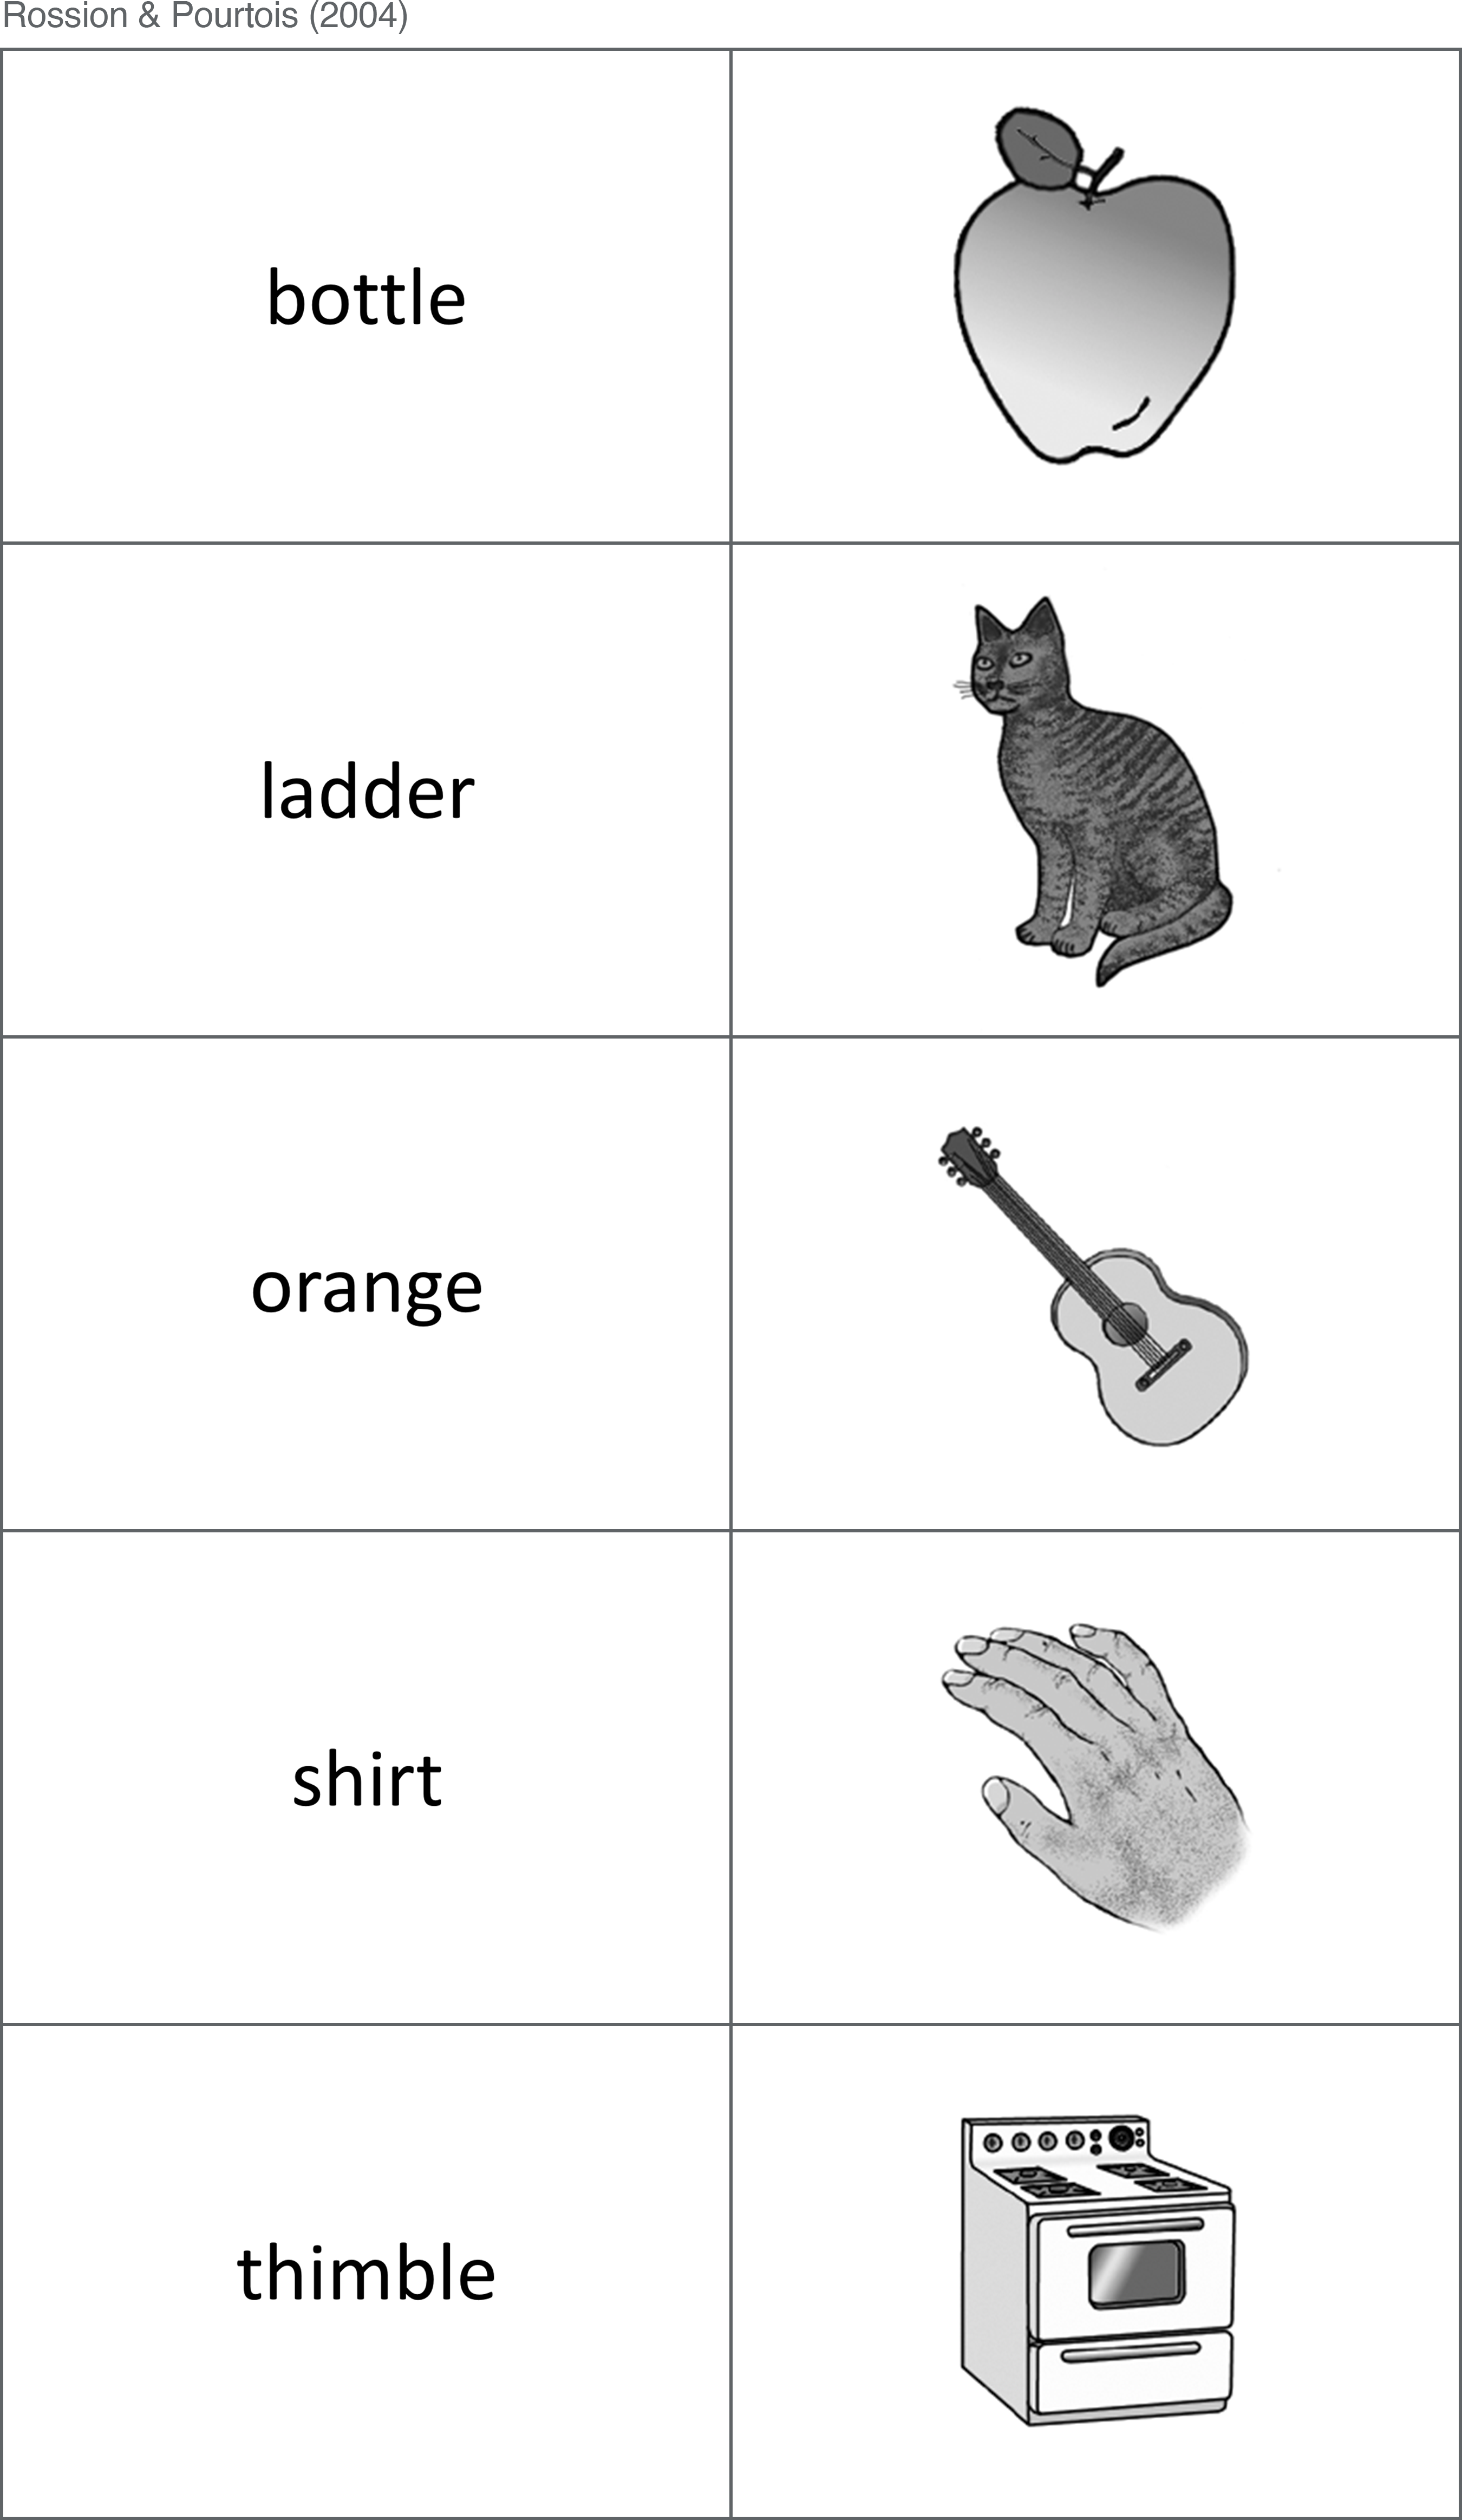
\includegraphics[width=1\linewidth]{./resources/images/exp1__stim_examples}
Figure 1: Example word and picture stimuli from the current study. ~ ~

\hypertarget{design}{%
\paragraph{Design}\label{design}}

\hfill\break The current study utilised a mixed design, with a 2-level
within-subjects factor of stimuli format (words, drawings), and a
3-level between-subjects factor of response option (RFG, RFBG,
RF-Ratings). Subjects completed two study blocks - one consisting only
of word stimuli, the other consisting only of picture stimuli - before
completing a single mixed format recognition test, where previously
studied word and picture items were randomly shown among new, unseen
items. Subjects passed through 2 levels of blocked randomization during
the experiment (equally sized, predetermined blocks). First, subjects
were randomly allocated into one of two study block orders, which
determined the order in which they were presented with the picture and
word blocks at study. Second, subjects were assigned into one of three
possible recognition tests (identical aside from the response options
available when categorising recognition experiences): 1) RFG:
``Recollection'', ``Familiarity'',``Guessing''; 2) RFBG:
``Recollection'', ``Familiarity'', ``Guessing'', ``Both'', or 3)
RF-Ratings: two independent 0-5 rating scales to separately report the
contribution of Recollection and Familiarity. These randomisation
processes were completed automatically by the experiment software using
balanced methods.

\hypertarget{procedure}{%
\paragraph{Procedure}\label{procedure}}

\hfill\break Data collection was conducted via the online survey
platform Qualtrics\footnote{\url{https://www.qualtrics.com/uk/}}.
Subjects initially completed an encoding block, where target words and
pictures were randomly presented one-at-a-time on-screen. To ensure
attention was directed to the presented stimuli, participants were
required to respond to a simple encoding question toward each item at
study: ``Is this a picture or a word?''. This question allowed for the
assessment of performance during the study block (to determine whether
participants were concentrating at study), whilst also avoiding
potential levels-of-processing effects that can accompany deeper
encoding judgements (e.g.~pleasantness ratings). The encoding phase was
followed by a short distractor task comprised of 20 multiplication sums.
Finally, subjects completed the recognition task, where they were again
randomly presented with word and picture items one-at-a-time on-screen,
and were required to respond \emph{Old}/\emph{New} depending on whether
they recognised the item or not. \emph{Old} responses were succeeded by
a follow-up screen whereby participants were asked to report their
recognition experience for the current item; the response options
available during this follow-up response page differed between
participants, with random allocation into either the RFG, RFBG, or
RF-Ratings response option conditions. Recollection and Familiarity were
defined identically across conditions, and the only deviations in
instructions were: i) to define the additional ``Both'' response option
in the RFBG condition; and ii) explain how certain responses should be
reported in the RF-Ratings condition (i.e.~subjects could still report a
``Guess'' in this condition by providing a 0-rating on both of the
scales).

\hypertarget{data-processing}{%
\paragraph{Data processing}\label{data-processing}}

\hfill\break Measured variables included the total number of hits and
FAs, and the total number of hits and FAs assigned to each of the
available response options (RFG, RFBG, and RF Ratings). In order to
create a common dependant variable, proportions were calculated from
these variables in slightly different ways depending on the response
option group. In the RFG-judgement group, simple proportions were
created from the total number of R responses and the total number of F
responses. In the RFBG condition, similar proportions were calculated by
separately adding the proportion of Both responses to the proportion of
R and proportion of F responses. In the RF-Ratings group, proportions of
R and F were calculated based on the number of responses scoring
+\textgreater3; a response was classified R when subjects rated between
3-5 on the ``Recollection'' scale (regardless of the Familiarity
rating), and a response was classified F when subjects rated between 3-5
on the ``Familiarity'' scale (regardless of the Recollection rating).
The scales therefore allowed for pure R responses (R=3-5 + F=0-2), pure
F responses (F=3-5 + R=0-2), both responses (R=3-5 + F=3-5) and Guessing
responses (R=0 + F=0). Additional DVs included: i) d' (d-prime, a signal
detection measure of sensitivity); ii) c-value (a measure of response
bias); iii) overall accuracy (hits / (hits + FAs)); iv) reaction times
for all responses.

All analyses were conducted with \emph{R} (R Core Team, 2020) using the
\emph{afex} (v0.28-0; Singmann, Bolker, Westfall, Aust, \& Ben-Shachar,
2020) and \emph{rstatix} packages (v0.6.0; Kassambara, 2020).

A series of exclusion criteria were defined before analysis. First,
subjects were to be excluded from analysis if they showed poor
performance during the encoding task; the relative ease of reporting
whether each item was shown as a word or picture prompted a performance
cut off of 90\% accuracy. This would allow for some accidental clicks,
though subjects scoring less than 90\% were to be excluded on the
assumption they did not dedicate their full attention to the task.
Second, subjects would be considered outliers (and thus excluded from
analysis) if they presented extreme z-scores of +/- 3 for total hits,
total FAs, or overall recognition (hits minus FAs). However, no subjects
were found to meet any of these criteria.

\hypertarget{results}{%
\subsubsection{Results}\label{results}}

\hypertarget{picture-superiority}{%
\paragraph{Picture superiority}\label{picture-superiority}}

To establish baseline picture superiority effects in the current
paradigm, and assess whether there were any interactions with the
availability of different response options options at test, a series of
2 (stimuli format: words, pictures) x 3 (response option option
condition: RFG-judgements, RFBG-judgements, RF-ratings) mixed ANOVAs
were conducted on a number of outcome variables. Namely, the signal
detection measures of \emph{d'} (sensitivity) and \emph{c} (decision
criterion), as well as the proportion of overall hits, false alarms
(FAs), and overall recognition (hits - FAs) {[}see Table 2{]}.
Significant main effects and interaction effects were followed-up with
Bonferroni-adjusted pairwise comparisons.

The ANOVA on \emph{d'} scores demonstrated a significant main effect of
stimuli-format, \emph{F}(1, 183) = 278.32, \emph{p} \textless{} .001,
\(\eta^2_p\) = .60, a PSE was evident, with pictures (\emph{M}= 1.73)
producing significantly better discrimination between hits and FAs than
words (\emph{M}= 0.92), \emph{t}(185) = 16.77, \emph{p} \textless{}
.001; \emph{d} = 1.23, 95\% CI {[}1.06, 1.44{]}. The ANOVAs on the
proportion of hits, FAs, and overall recognition also produced findings
consistent with a PSE. For hits, there was a significant main effect of
stimuli-format, \emph{F}(1, 183) = 131.77, \emph{p} \textless{} .001,
\(\eta^2_p\) = .42, with pictures (\emph{M}= 0.62) showing a higher
number of overall hits compared to words (\emph{M}= 0.47), \emph{t}(185)
= 11.55, \emph{p} \textless{} .001; \emph{d} = 0.85, 95\% CI {[}0.68,
1.05{]}. Similarly, the ANOVA on the proportion of FAs showed a
significant main effect of stimuli-format, \emph{F}(1, 183) = 61.18,
\emph{p} \textless{} .001, \(\eta^2_p\) = .25, with pictures (\emph{M}=
0.12) producing significantly fewer FAs than words (\emph{M}= 0.21),
\emph{t}(185) = -7.81, \emph{p} \textless{} .001; \emph{d} = -0.57, 95\%
CI {[}-0.69, -0.45{]}. No interaction effects were found between stimuli
format and response option for any of the variables.

Taken together, the findings demonstrate a replication of the PSE in the
current memory paradigm, and suggest stimuli format plays a key role in
memorability that is independent from the particular response options
available to participants. The current findings support the hypotheses
of a PSE manifesting as i) higher overall d' scores for pictures
compared to words, ii) a higher proportion of correct hits, iii) lower
proportion of false alarms, and iv) better overall recognition.

Table 2: Mean proportion of hits, FAs, and mean \emph{d'} scores, by
stimuli format and response option condition. Signif. codes: ***\emph{p}
\textless{} .001; **\emph{p} \textless{} .01; *\emph{p} \textless{} .05;
+ involved in significant interaction.

\begin{table}[!h]
\centering
\begin{tabular}{>{\raggedright\arraybackslash}p{3.6cm}>{\raggedright\arraybackslash}p{1.2cm}>{\centering\arraybackslash}p{1.2cm}>{\centering\arraybackslash}p{1.2cm}>{}p{1.2cm}>{}p{2cm}}
\toprule
  & Hits & FAs & d'\\
\midrule
\addlinespace[0.3em]
\multicolumn{4}{l}{\textbf{Stimuli format}}\\
\hspace{1em}Words & 0.47 & 0.21 & 0.92\\
\hspace{1em}Pictures & 0.62 & 0.12 & 1.73\\
\addlinespace[0.3em]
\multicolumn{4}{l}{\textbf{Response option}}\\
\hspace{1em}RFG & 0.62 & 0.19 & 1.44\\
\hspace{1em}RFBG & 0.54 & 0.16 & 1.28\\
\hspace{1em}RF-Ratings & 0.48 & 0.14 & 1.24\\
\bottomrule
\end{tabular}
\end{table}

\hypertarget{pse-in-rates-of-recollection-and-familiarity}{%
\paragraph{PSE in rates of Recollection and
Familiarity:}\label{pse-in-rates-of-recollection-and-familiarity}}

To determine the impact of stimuli format on the rates of R and F,
additional 2 (words, pictures) x 3 (RFG-judgements, RFBG-judgements,
RF-ratings) mixed ANOVAs were conducted on the mean proportion of hits
(see Figure 2) and FAs (see Figure 3) assigned R, F, and G.

\textbf{Recollection (hits):} For R hits, there was a significant
interaction between stimuli format and response option option condition,
\emph{F}(2, 183) = 3.62, \emph{p} = .029, \(\eta^2_p\) = .04 (see Figure
4).

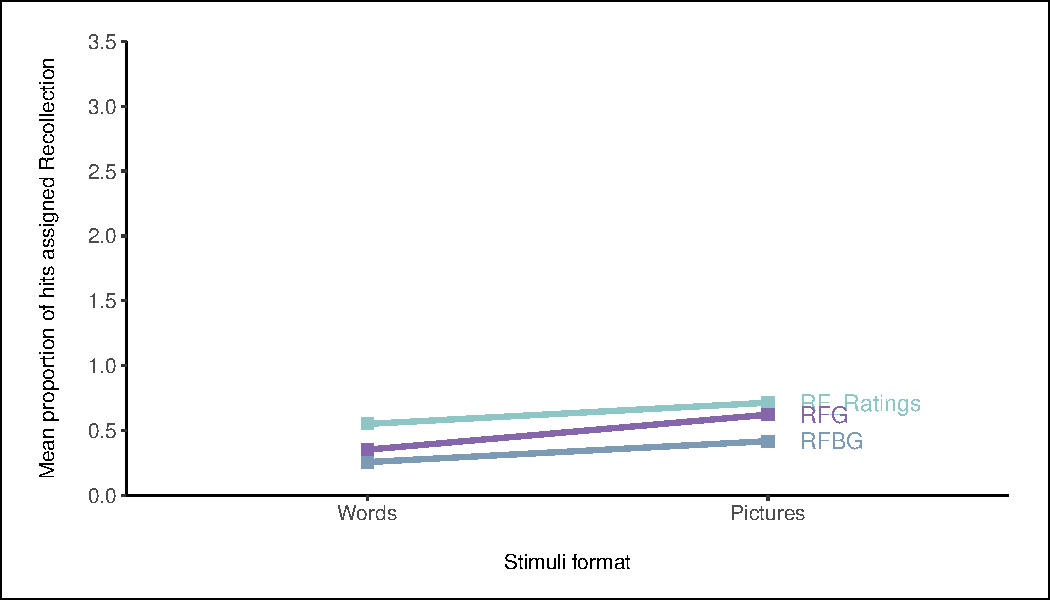
\includegraphics{R--Thesis_files/figure-latex/unnamed-chunk-11-1.pdf}
Figure 4: Interaction plot between stimuli format and response option
for the mean proportion of hits assigned Recollection.

Pictures produced a higher proportion of hits assigned
\emph{Recollection} than words in the RFG group (words {[}\emph{M}=
0.35{]} vs.~pictures {[}\emph{M}= 0.62{]}, \emph{t}(183) = -8.18,
\emph{p} \textless{} .001), RFBG group (words {[}\emph{M}= 0.25{]}
vs.~pictures {[}\emph{M}= 0.42{]}, \emph{t}(183) = -5.09, \emph{p}
\textless{} .001) and RF-Ratings group (words {[}\emph{M}= 0.55{]}
vs.~pictures {[}\emph{M}= 0.71{]}, \emph{t}(183) = -5.12, \emph{p}
\textless{} .001).

The interaction is evident following comparisons of the same stimuli
format across response option conditions. For words, the proportion of R
hits was significantly higher in the RF-Ratings group compared to both
the RFG group (RFG {[}\emph{M} = 0.35{]} vs.~RF-Ratings {[}\emph{M} =
0.55{]}, \emph{t}(279.16) = 4.07, \emph{p} = .001) and the the RFBG
group (RFBG {[}\emph{M} = 0.25{]} vs.~RF-Ratings {[}\emph{M} = 0.55{]},
\emph{t}(279.16) = 6.15, \emph{p} \textless{} .001). The RFG and RFBG
groups did not significantly differ in the proportion of word hits
assigned \emph{Recollection} (RFG {[}\emph{M} = 0.35{]} vs.~RFBG
{[}\emph{M} = 0.25{]}, \emph{t}(279.16) = -1.97, \emph{p} = .755).

For pictures, the RF-Ratings group again showed a significantly higher
proportion of R hits than the RFBG group (RFBG {[}\emph{M} = 0.42{]}
vs.~RF-Ratings {[}\emph{M} = 0.71{]}, \emph{t}(279.16) = 6.20, \emph{p}
\textless{} .001). While words produced a significant difference between
the RFG and RF-Ratings group for R hits, the same was not found for
pictures (RFG {[}\emph{M} = 0.62{]} vs.~RF-Ratings {[}\emph{M} =
0.71{]}, \emph{t}(279.16) = 1.89, \emph{p} = .900). Instead, the RFG
group also produced a significantly higher proportion of R hits than the
RFBG group (RFG {[}\emph{M} = 0.62{]} vs.~RFBG {[}\emph{M} = 0.42{]},
\emph{t}(279.16) = -4.20, \emph{p} = .001).

\textbf{Familiarity (hits):} For F hits, there was a significant
interaction between stimuli format and response option option condition,
\emph{F}(2, 183) = 28.27, \emph{p} \textless{} .001, \(\eta^2_p\) = .24
(see Figure 5).

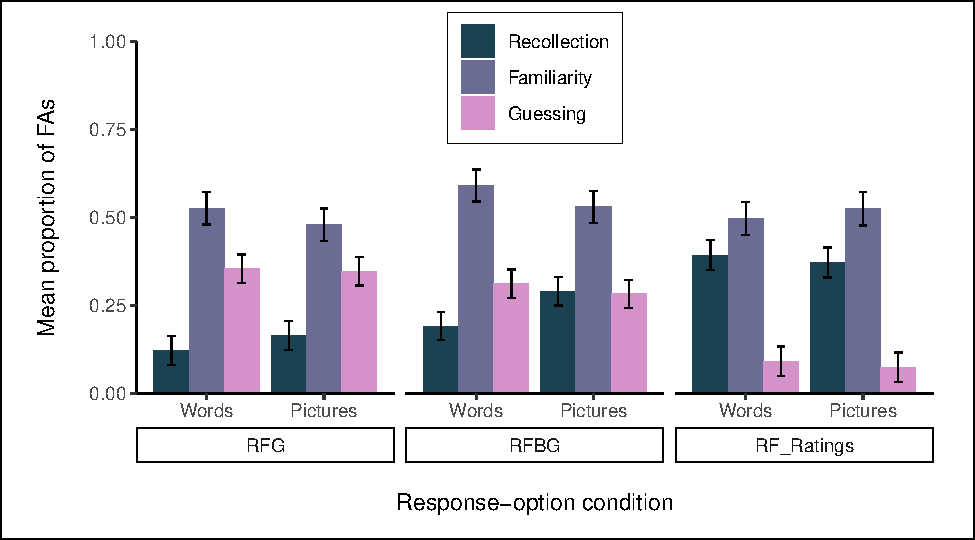
\includegraphics{R--Thesis_files/figure-latex/unnamed-chunk-14-1.pdf}
Figure 5: Interaction plot between stimuli format and response option
for the mean proportion of hits assigned Recollection.

Pictures produced a higher proportion of hits assigned
\emph{Familiarity} than words in the RF-Ratings group only (words
{[}\emph{M}= 0.63{]} vs.~pictures {[}\emph{M}= 0.78{]}, \emph{t}(183) =
-4.62, \emph{p} \textless{} .001). In both the RFG and RFBG groups,
words produced a higher proportion of hits assigned \emph{Familiarity}
than pictures (RFG: words {[}\emph{M}= 0.48{]} vs.~pictures {[}\emph{M}=
0.3{]}, \emph{t}(183) = 5.41, \emph{p} \textless{} .001; RFBG: words
{[}\emph{M}= 0.38{]} vs.~pictures {[}\emph{M}= 0.27{]}, \emph{t}(183) =
3.36, \emph{p} = .014).

Comparisons of the same stimuli format across response option conditions
showed that, for words, the proportion of F hits was significantly
higher in the RF-Ratings group compared to both the RFG group (RFG
{[}\emph{M} = 0.48{]} vs.~RF-Ratings {[}\emph{M} = 0.63{]},
\emph{t}(302.47) = 3.31, \emph{p} = .016) and the the RFBG group (RFBG
{[}\emph{M} = 0.38{]} vs.~RF-Ratings {[}\emph{M} = 0.63{]},
\emph{t}(302.47) = 5.56, \emph{p} \textless{} .001). The RFG and RFBG
groups did not significantly differ in the proportion of word hits
assigned \emph{Familiarity} (RFG {[}\emph{M} = 0.48{]} vs.~RFBG
{[}\emph{M} = 0.38{]}, \emph{t}(302.47) = -2.14, \emph{p} = .499).

For pictures, the RF-Ratings group again showed a significantly higher
proportion of F hits than both the RFG group (RFG {[}\emph{M} = 0.3{]}
vs.~RF-Ratings {[}\emph{M} = 0.78{]}, \emph{t}(302.47) = 10.70, \emph{p}
\textless{} .001) and the RFBG group (RFBG {[}\emph{M} = 0.27{]}
vs.~RF-Ratings {[}\emph{M} = 0.78{]}, \emph{t}(302.47) = 11.44, \emph{p}
\textless{} .001). Similar to words, the RFG and RFBG groups did not
significantly differ in the proportion of F hits produced by pictures
(RFG {[}\emph{M} = 0.3{]} vs.~RFBG {[}\emph{M} = 0.27{]},
\emph{t}(302.47) = -0.50, \emph{p} \textgreater{} .999).

\textbf{Guessing (hits):} For G hits, there was a significant
interaction between stimuli format and response option option condition,
\emph{F}(2, 183) = 3.99, \emph{p} = .020, \(\eta^2_p\) = .04 (see Figure
6).

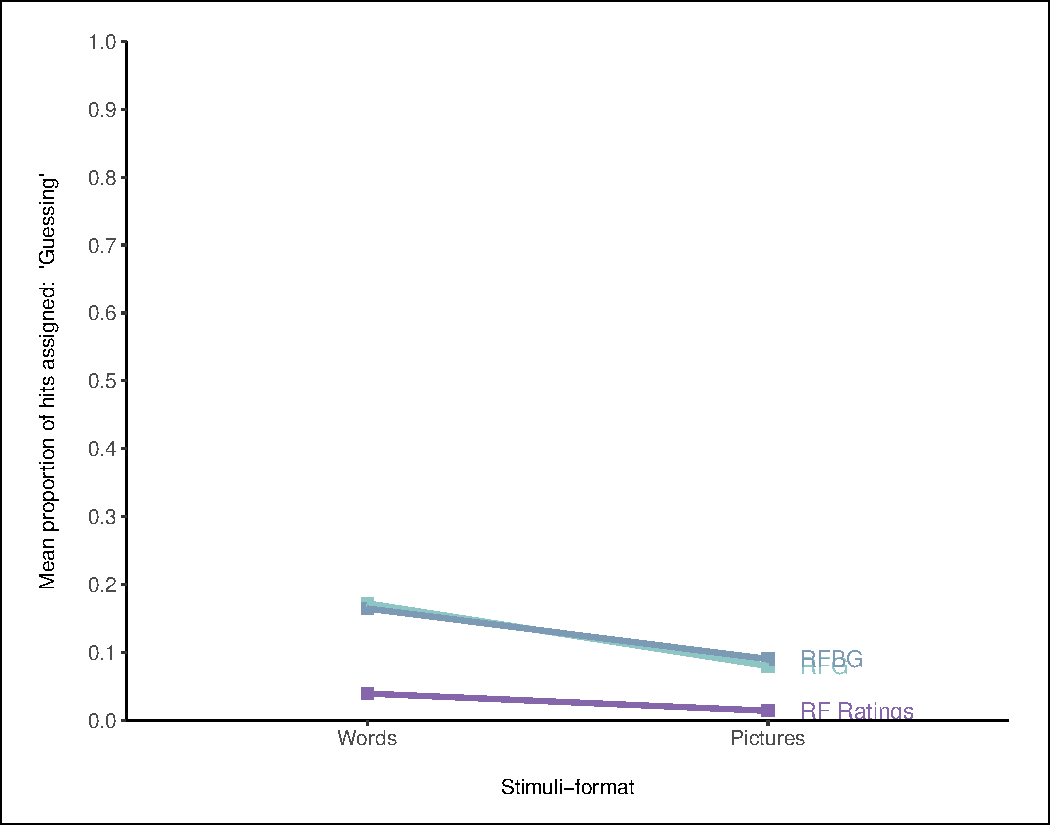
\includegraphics{R--Thesis_files/figure-latex/unnamed-chunk-17-1.pdf}
Figure 6: Interaction plot between stimuli format and response option
for the mean proportion of hits assigned Recollection.

Words produced a higher proportion of hits assigned \emph{Guessing} than
pictures in both the RFG group (words {[}\emph{M}= 0.17{]} vs.~pictures
{[}\emph{M}= 0.08{]}, \emph{t}(183) = 5.28, \emph{p} \textless{} .001)
and RFBG group {[}\emph{M}= 0.16{]} vs.~pictures {[}\emph{M}= 0.09{]},
\emph{t}(183) = 4.26, \emph{p} \textless{} .001). Words and pictures did
not significantly differ in RF-Ratings group (words {[}\emph{M}= 0.04{]}
vs.~pictures {[}\emph{M}= 0.01{]}, \emph{t}(183) = 1.51, \emph{p}
\textgreater{} .999).

Comparisons of the same stimuli format across response option conditions
showed that, for words, the proportion of G hits was significantly lower
in the RF-Ratings group compared to both the RFG group (RFG {[}\emph{M}
= 0.17{]} vs.~RF-Ratings {[}\emph{M} = 0.04{]}, \emph{t}(286.62) =
-5.56, \emph{p} \textless{} .001) and the RFBG group (RFBG {[}\emph{M} =
0.16{]} vs.~RF-Ratings {[}\emph{M} = 0.04{]}, \emph{t}(286.62) = -5.03,
\emph{p} \textless{} .001). The RFG and RFBG groups did not
significantly differ in the proportion of word hits assigned
\emph{Guessing} (RFG {[}\emph{M} = 0.17{]} vs.~RFBG {[}\emph{M} =
0.16{]}, \emph{t}(286.62) = -0.64, \emph{p} \textgreater{} .999).

For pictures, the RF-Ratings group again showed a significantly lower
proportion of G hits than the RFBG group (RFBG {[}\emph{M} = 0.09{]}
vs.~RF-Ratings {[}\emph{M} = 0.01{]}, \emph{t}(286.62) = -3.15, \emph{p}
= .027), however, the comparison with the RFG group did not reach
significance (RFG {[}\emph{M} = 0.08{]} vs.~RF-Ratings {[}\emph{M} =
0.01{]}, \emph{t}(286.62) = -2.89, \emph{p} = .063). Again, the RFG and
RFBG groups did not significantly differ in the proportion of G hits
produced by pictures (RFG {[}\emph{M} = 0.08{]} vs.~RFBG {[}\emph{M} =
0.09{]}, \emph{t}(286.62) = 0.20, \emph{p} \textgreater{} .999).

Such findings mostly support the proposed hypotheses. Pictures indeed
produced a higher proportion of R hits in comparison to words, though no
picture superiority was evident in the number of R FAs. This suggests
that, despite words showing a decreased level of memorability compared
to pictures, they do not elicit high certainty false recognition at any
higher rate. Words also produced a higher proportion of F hits compared
to pictures, as predicted, but only in the RFG and RFBG conditions. It
is unclear why the same pattern was not evident in the RF-Ratings group,
aside from the possibility that participants avoided the more complex
ratings screen (and instead more often chose \emph{New}, inaccurately),
unless they had a high certainty of their recognition (as evidenced for
R hits). Again, there was no evidence of picture superiority in regard
to the number of F FAs. The hypotheses put forward for G responses were
again mostly supported; there were more guesses made toward words than
pictures, however, this again only applied to the RFG and RFBG
conditions. Such findings align with the possible explanation outlined
above, whereby participants avoided having to provide two separate
ratings unless they were very certain they recognised the item.

\hypertarget{discussion}{%
\subsubsection{Discussion}\label{discussion}}

\hfill\break The aim of the current study was to establish baseline PSE
response patterns in a novel, modified RK paradigm. Substituting the
classic \emph{Remember} / \emph{Know} labels for \emph{Recollection} /
\emph{Familiarity}, recognition for words and pictures was tested across
three separate response option conditions (RFG, RFBG, RF-Ratings).
Analysis of the behavioural data demonstrated a clear Picture
Superiority Effect (PSE) in the current paradigm, with picture stimuli
showing better discrimination, a higher number of overall hits, lower
number of FAs, and better overall recognition performance than words.
Taken together, these findings are consistent with the notion that
pictures offer an enhanced memorability in comparison to words. When
word stimuli were correctly identified, they were not recognised in the
the same context-rich nature as pictures, evidenced by a higher
proportion of F responses. The current findings also align with those
from previous studies, with pictures showing enhanced recollection
(Curran \& Doyle, 2011; Rajaram, 1996a) and words showing enhanced
familiarity (Ally \& Budson, 2007). While most of the proposed
hypotheses were supported, there were some unexpected results. Stimuli
format had no effect on the obtained proportions of FAs; regardless of
whether FAs were assigned R or F, there was no evidence of picture
superiority. This finding does not refute the notion of a PSE in the
current paradigm - the memorial advantage of pictures over words is
evident, but it instead indicates that stimuli without this advantage
(i.e.~words) may produce more misses, but not increased levels of false
recognition.

Many of the unexpected results are centred around the RF-Ratings
response option condition. Word stimuli were hypothesised to produce
more Familiarity and Guessing hits than pictures, since it was expected
that they would not be recognised in the the same context-rich nature as
pictures. This result was indeed obtained in both the RFG and RFBG
response-option conditions, however, the RF-Ratings did not produce the
same finding (no difference between stimuli formats was observed).
Similarly, while the RFG and RFBG conditions showed comparable
proportions of hits and levels of response bias (\emph{c} scores), the
RF-Ratings group again produced different findings, showing
significantly fewer hits and significantly higher \emph{c} scores (and
thus a more conservative response bias) compared to the RFG group. As
the proportion of hits and mean \emph{c} scores were not significantly
different between the RF-Ratings and RFBG response option groups, it
indicates that these results may be attributable to participants having
the ability to report that they experience \emph{Both} recollection and
familiarity processes conjointly. However, as performance differences
were most notable in the RF-Ratings condition, it suggests these
findings are attributable to the increased task complexity from RFG to
RFBG, and RFBG to RF-Ratings. The option to report \emph{Both} may be
confusing to participants, especially to those who struggle to
understand the distinction between recollection and familiarity to begin
with (Geraci et al., 2009; Rubin \& Umanath, 2015; Williams \& Moulin,
2014). Providing the \emph{Both} option in the form of two scales may
exacerbate this confusion further, and thus lead to results that are
significantly different from the condition with the least complexity
(RFG). Such a hypothesis is supported by a number of other findings.
First, the more conservative response bias exhibited by those in the
RF-Ratings group demonstrates how subjects were less likely to respond
\emph{Old} when they were required to provide more detailed follow-up
recognition judgements (i.e., using separate 0-5 scales for R and F),
compared to simply selecting one of three options (R,F, or G). Second,
despite \emph{Guessing} responses being permissible in any of the
response-option groups, participants were significantly less likely to
report a guess when two independent ratings were required - a finding
evident from the reduced number of \emph{Guessing} hits and FAs compared
to the other response option conditions. Third, the RF-Ratings group
showed significantly more R hits and R FAs compared to both the
RFG-group and the RFBG-groups, indicating participants were more likely
to respond \emph{Old} in the RF-Ratings condition when they experienced
high certainty in their recognition - regardless of whether or not that
recognition was accurate or false. Taken together, these findings all
support the notion of a certain level of avoidance from participants
when they were required to provide more detailed reports of their
recognition.

Establishing baseline PSEs in the current paradigm is important for
allowing further experimental manipulations in the experiments that
follow. While the independent ratings paradigm proposed by Higham \&
Vokey (2004) is undoubtedly useful in the discussion around the most
effective methods of measuring recollection and familiarity, it does not
suit the needs of current programme of research going forward, where
comparisons between different stimuli formats is the primary concern. In
the current experiment, picture stimuli consisted of simple greyscale
illustrations (Rossion \& Pourtois, 2004), though the extent to which
stimuli of increasing levels of detail impacts recognition is unclear.
The distinctiveness of to-be-remembered stimuli will be systematically
compared across a number of experiments, following the conception of a
new set of detailed realistic photograph stimuli. Following the unique
results obtained from the RF-Ratings group in the current experiment, it
is likely that this condition would exhibit further differences if
included in the proposed experiments, which may become difficult to
interpret when further stimuli formats are introduced. The current
findings to suggest avoidant response patterns in the RF-Ratings group
further highlight the unique results this condition might produce.
Therefore, only the RFG and RFBG response option conditions will be
taken forward into the proposed recognition experiments that focus on
comparisons of stimuli distinctiveness.

\#\#\#\#\#\#----------------------------------------

\newpage

\hypertarget{chapter-3}{%
\section{Chapter 3}\label{chapter-3}}

\hypertarget{background-1}{%
\subsection{Background}\label{background-1}}

The Picture Superiority Effect (PSE) is a highly robust and replicable
phenomenon. In recognition memory paradigms, the PSE has been shown to
manifest as both increased recollection and familiarity (Dewhurst \&
Conway, 1994; Rajaram, 1993, 1996b; Wagner, Gabrieli, \& Verfaellie,
1997; Yonelinas, 2002). The effect is present in children, adolescents
and healthy older adults (Whitehouse, Maybery, \& Durkin, 2006), though
perhaps more striking is the fact that patients with Alzheimer's disease
or those presenting early isolated memory impairments, known as amnestic
mild cognitive impairment (aMCI), also show memorial benefits toward
pictures (Ally, 2012). This is supported by ERP studies demonstrating
comparable enhancements to recollection-based ERP components between
healthy older and aMCI groups when pictures, rather than words, are
utilised (Ally et al., 2009a). There is debate within the literature
attempting to characterise the nature of memory deficits in aMCI,
whereby despite general agreement that recollection processes are
impaired in such individuals, findings show great inconsistency with
regard to familiarity (Algarabel et al., 2012; Belleville et al., 2011;
Pitarque, 2016; Wolk, Dunfee, Dickerson, Aizenstein, \& DeKosky, 2011;
Wolk, Mancuso, Kliot, Arnold, \& Dickerson, 2013). The PSE may have been
largely overlooked as an area for further research in an effort to help
settle this debate, despite recent reviews highlighting methodological
differences across studies as the potential source of inconsistent
findings (Koen \& Yonelinas, 2014; Migo et al., 2012; Schoemaker et al.,
2014). The level at which stimuli distinctiveness impacts successful
recognition is currently unclear, and there is little consistency across
studies with regard to what is considered a `picture'.

Many experiments utilise illustrations for their picture stimuli (van
der Meulen et al., 2012; Westerberg et al., 2013; Wolk et al., 2011),
with a standardised set of items published by Snodgrass \& Vanderwart
(1980) among the most-used illustrated picture stimuli within the domain
of memory research (Bermúdez-Margaretto, Beltrán, Cuetos, \& Domínguez,
2018; Deason, Hussey, Flannery, \& Ally, 2015; Hockley, 2008; Martins \&
Lloyd-Jones, 2006; McBride \& Anne Dosher, 2002; Meade, Ahmad, \&
Fernandes, 2019; Schmitter-Edgecombe, Woo, \& Greeley, 2009; van der
Meulen et al., 2012; Wagner et al., 1997; Wammes, Meade, \& Fernandes,
2016; Weldon, Iii, \& Challis, 1989; Weldon \& Roediger, 1987;
Whitehouse et al., 2006). The set consists of 260 line drawings of
common, everyday objects (in black ink), along with their written word
counterpart (e.g.~``shoe''). Items were selected on the basis of
exemplifying a number of semantic categories, including animals,
furniture, fruit, etc., and a range of normative data was collected for
each item; indices of naming agreement, mental imagery agreement, visual
complexity, and familiarity were all recorded for each drawing. The
normative data for the Snodgrass \& Vanderwart (1980) items has been
continually revisited, with a number of studies gathering
culturally-appropriate norms (e.g.~in Spanish (Sanfeliu \& Fernandez,
1996), Chinese (Yoon et al., 2004), and Russian (Tsaparina, Bonin, \&
Méot, 2011), and additional testing of the relationship between reaction
time and naming agreement (Székely et al., 2003). There are multiple
theories of object recognition; the recognition-by-components theory
proposed by Biederman (1987) identifies shape as the most crucial factor
for successful recognition, in which case, the object outlines found in
the set by Snodgrass \& Vanderwart (1980) should be more than sufficient
for experimental cognitive research. Other theories, however, posit that
surface details such as colour and texture are just as crucial in
forming object representations (Tanaka, Weiskopf, \& Williams, 2001;
Tarr \& Bülthoff, 1998). The wide-ranging applicability of the Snodgrass
\& Vanderwart (1980) items throughout a number of cognitive disciplines
has led to a more recent revision of the items by Rossion \& Pourtois
(2004). This revision consists of the exact same objects, digitally
re-drawn to include surface textures and shading. Additionally, this set
provides greyscale and colour versions for all items, as opposed to the
greyscale-only items found in the Snodgrass \& Vanderwart (1980) set
(see Figure 7 for example items contained in the Snodgrass \& Vanderwart
(1980) and Rossion \& Pourtois (2004) stimuli sets). The Rossion \&
Pourtois (2004) revision now appears to be favoured over the original
Snodgrass \& Vanderwart (1980) set among many cognitive researchers
(Rollins \& Riggins, 2018, p. @ensor2019b; Stenberg, 2006; Wolk et al.,
2008), almost certainly attributable to the increased detail and ability
to choose whether colour is a necessary condition.

Despite their widespread use, line drawings have been criticised for
their relative simplicity and lack of realism (Viggiano, Vannucci, \&
Righi (2004)), with many researchers favouring the use of photographs as
experimental stimuli (Embree et al., 2012; Pitarque, 2016; Troyer et
al., 2012; Troyer, Vandermorris, \& Murphy, 2016; P. Wang et al., 2013).
Photographs of faces are especially useful in research examining emotion
and face recognition (Barba, 1997; Bowen, Fields, \& Kensinger, 2019;
Cui et al., 2016; Herzmann, Minor, \& Curran, 2018), though a number of
common-object photograph sets have also emerged as ecological
alternatives to line-drawn items (Adlington, Laws, \& Gale, 2009;
Moreno-Martínez \& Montoro, 2012; Viggiano et al., 2004). While the
published sets of photographs are undoubtedly useful in a range of
cognitive domains, they do not allow us to specifically examine stimuli
format as a factor on its own, as the concepts depicted are unique to
the set they derive from. In order to make such comparisons, and ensure
any differences in performance (e.g.~recognition memory ability) are
indeed attributable to stimuli format, the objects depicted must be
consistent across stimuli formats. The current study presents a new set
of photographic stimuli that extend the set of words and drawings
provided by Rossion \& Pourtois (2004), wherein each of the concepts
depicted has been carefully matched across formats. These new stimuli
will be utilised throughout a number of planned recognition experiments
that aim to systematically compare measures of recognition against
different `levels' of stimuli. The curation of a new set of photographs
- carefully matched to other formats - allows investigation into whether
picture superiority magnitudes are mediated by the format pictures are
presented in. The inconsistent use of different formats across studies
has previously made it difficult to reconcile effects obtained in
response to drawings with those obtained in response to photographs - an
inherent problem when concepts are not matched across format. Normative
data for the new set of photographs is also presented, allowing others
who also wish to use our photograph stimuli to filter items by measures
of naming agreement, mental imagery agreement, familiarity, visual
complexity, and colour diagnosticity.

~ ~

\includegraphics[width=1\linewidth]{./resources/images/exp2__stim_examples}
~ ~ Figure 8: Examples of matching pictures across Snodgrass \&
Vanderwart (1980), Rossion \& Pourtois (2004), and photographs from the
current study. Greyscale versions of the drawings and photographs are
not presented in this example. ~ ~

\hypertarget{experiment-development-of-a-new-set-of-standardised-photographic-stimuli}{%
\subsection{Experiment: Development of a new set of standardised
photographic
stimuli}\label{experiment-development-of-a-new-set-of-standardised-photographic-stimuli}}

\newpage

\hypertarget{method-1}{%
\subsubsection{Method}\label{method-1}}

\hypertarget{participants-1}{%
\paragraph{Participants}\label{participants-1}}

A total of 377 subjects completed the online experiment (see Table 3 for
a breakdown of the gender and age of the sample). This sample size
provided 20 data points for each of the five response types, while also
ensuring the experiment did not last too long for participants (approx
25-mins). Subjects were recruited from both voluntary participation
websites such as
Prolific Academic\footnote{\url{https://www.prolific.co/}} (where they
received payment at the rate of £5/hr), and via the in-school
research participation system\footnote{\url{https://keelepsychology.sona-systems.com/}}
(where they received course participation credits).

Table 3: Gender and age (\emph{SD}) of the current sample.

\begin{table}[!h]
\centering
\begin{tabular}{l>{}rr>{}l}
\toprule
Gender & N & Age & \\
\midrule
Female & \em{196} & 33.22 & \em{(11.28)}\\
Male & \em{171} & 33.15 & \em{(10.3)}\\
Non-binary & \em{2} & 23.50 & \em{(-)}\\
Unspecified & \em{5} & 29.40 & \em{(6.11)}\\
\textbf{Total} & \textbf{\em{377}} & \textbf{NA} & \textbf{\em{NA}}\\
\bottomrule
\end{tabular}
\end{table}

To meet our YA requirements, all participants were required to be aged
between 18-59 years (actual obtained range: 18-59 years). As our
experiment involved typing the English labels for a range of image
stimuli, subjects were also asked whether English was their first
language; all but one participant indicated that English was indeed
their first language (99.2\%).

\hypertarget{materials-1}{%
\paragraph{Materials}\label{materials-1}}

A pool of 136 shaded drawings (Rossion \& Pourtois, 2004) - depicting
common, everyday objects - were brought forward from the previous
experiment. These items (along with their written-word labels) would
form two of the unique stimuli formats that would be used in future
recognition experiments (words and drawings). In this study, the
drawings from Rossion \& Pourtois (2004) were simply used as a reference
in the photograph matching process. Corresponding photographs were
obtained online with the aim of depicting the everyday objects in a
similar manner to the drawings. The inherent subjectivity involved in
this process may have led to images that were not a reliable `match' to
the concepts they were selected to depict (for example, the photograph
chosen to depict the concept ``bottle'' may inadvertently provoke the
majority of participants to give the label ``wine'', thus indicating
that this particular photograph fails to accurately depict the intended
concept). To address this issue, and ensure all photographs more
objectively depict the same concepts as the shaded drawings, three
different photograph variations were found for each everyday object,
with the aim of taking the best `match' forward. An emphasis was placed
on variety across these variations, with the aim of obtaining at least
one photograph that very closely resembled the line-drawn depiction, and
another offering a more modern depiction. Some items were substituted
due to unique restrictions that meant they could not easily be
translated into photographic format (for example, the shapes ``arrow''
and ``star'' can not be represented similarly as photographs). Photo
stimuli were obtained by searching open-source, copyright-free image
websites (e.g.~Unsplash\footnote{\url{https://unsplash.com/}};
Pexels\footnote{\url{https://www.pexels.com/}}) for photographs that
depicted the same everyday objects as the shaded drawings (see Appendix
B for the full list of image references).

The matching process produced a total of 408 unique photographs. All
were imported into Adobe Photoshop (20.0.04 Release), where the
background was removed to isolate the object of interest from other
potentially distracting visual details. This was completed manually
using the magnetic lasso and polygonal lasso tools (edges were either
feathered by 1px or left un-feathered). The orientation of isolated
objects was adjusted to ensure they matched as closely as possible with
their line-drawn counterpart (e.g.~all photograph variations of the item
`boot' were adjusted so the toe was facing left and the heel facing
right, as in the shaded drawing); this was often achieved by flipping or
mirroring the object to `correct' the direction.

Despite isolating objects from their background, a small number of
photographs still contained irrelevant and potentially distracting
details. For example, in one photograph variation of the item `piano',
there was a sign on the object that may have impacted how the item was
named or rated. Such details were removed as best as possible using the
clone stamp and content-aware fill tools. Any obvious text (e.g.~brand
names) and numbers were also removed from photographs using the same
method (see Figure 9). The primary aim of the current study was to
obtain photographs that could be clearly distinguished as a unique
stimuli format among words and shaded drawings; it is conceivable that
combining these formats (i.e.~inadvertently including photographs that
also contain written words) might affect recognition performance in ways
that are not directly comparable to items defined only by a single
category. Any text in our photographs was therefore removed, apart from
a couple of exceptions whereby such details happened to be integral to
the depiction of the object (e.g.~the numbers found on a ruler or
clock).

All photographs were exported from Photoshop in ``.png'' format in both
their original colour and in greyscale (by setting saturation levels to
0). Final edits were completed in Adobe Lightroom (Classic, 8.2
Release): exposure (brightness) adjustments were made on images that
appeared too light or too dark; highlights were decreased if some areas
were too bright compared to the rest of the photograph; shadows were
raised if some areas were too dark compared to the rest of the
photograph; noise reduction was applied to some items after isolating
the subject had inadvertently made unwanted noise/grain more visible.
The changes made to each image were systematically applied to both the
colour and greyscale versions (e.g.~if one variation of ``shoe'' had an
exposure increase of .010 for the colour version, the greyscale version
also received an exposure increase of .010). Some colour-specific
adjustments were made to the colour photographs only, however; common
photo artefacts such as chromatic aberration (purple fringing) were
corrected, along with white balance normalisation. Finally, all
photographs were placed on a 600x600 pixel white background, and made to
fill this frame as much as possible (i.e.~some items were restrained by
height, whilst others were restrained by width).

~ ~

\includegraphics[width=1\linewidth]{./resources/images/photo-manipulation-examples}
~ ~ Figure 9: Examples of background and text removal in photograph
items. ~ ~

\hypertarget{design-1}{%
\paragraph{Design}\label{design-1}}

This was a descriptive study; a mix of qualitative and quantitative data
were gathered. Across three blocks, all participants provided five types
of response toward photograph stimuli: i) Naming; ii) Familiarity; iii)
Visual Complexity, iv) Colour Diagnosticity; and v) Mental Imagery
Agreement. Excluding the Naming task (consisting of a typed single-word
answer), all responses were provided on a 5-point ordinal scale. Within
participants, the maximum number of response type provided for any one
item was two; Naming and Familiarity responses were paired in one block,
Visual Complexity and Colour Diagnosticity responses were paired in
another, and Mental Imagery Agreement responses were always presented in
a separate block. The order of these three blocks was counterbalanced
across participants. Toward each individual photograph, participants
made only one or two types of response before moving on to the next
item, and the same items were not repeated to participants. For each
photograph, the five types of required data were obtained by
counterbalancing between participants (e.g.~for the first variation of
the ``cat'' photograph, the Naming and Familiarity data was obtained
from one participant, the Visual Complexity and Colour Diagnosticity
data was obtained from another, and the Mental Imagery Agreement data
was obtained from another).

\hypertarget{procedure-1}{%
\paragraph{Procedure}\label{procedure-1}}

Data collection was conducted via two online platforms; i)
Qualtrics\footnote{\url{https://www.qualtrics.com/uk/}} - a survey
platform that allowed for straightforward collection of consent,
demographics, and computer compatibility data, and ii)
Pavlovia\footnote{\url{https://pavlovia.org/}} - an open-source
experiment hosting platform for studies programmed in Javascript (Peirce
et al., 2019).

In the Naming and Familiarity block, participants were first asked
``What is the name of the item depicted?''. Subjects were instructed to
name each photograph as briefly and unambiguously as possible, with one
name only, and respond by typing their answer into the response box. If
they did not know the name of an item, or had a tip-of-the-tongue
experience, participants were instructed to type ``no'' for their answer
(the term ``don't know'' was avoided so as not to encourage subjects to
deviate from single-word responses, as instructed).Following the naming
judgement, with the same photograph still present on-screen,
participants were next asked ``How familiar is the item depicted?''.
Subjects were instructed to judge each photo according to how usual or
unusual the item was in their realm of experience; specifically,
familiarity was defined as ``the degree to which you come in contact
with, or think about, the concept'', and encouraged participants to rate
the concept itself rather than the particular way it was currently
shown. Participants selected one value from the 5-point scale, ranging
from very unfamiliar (1) to very familiar (5), and were encouraged to
use the full range of the scale throughout the set of photographs.

In the Visual Complexity and Colour Diagnosticity block, participants
were first instructed to respond to the question ``How visually complex
is this picture?'' using a 5-point scale that ranged from ``very
simple'' (1) to ``very complex'' (5). Complexity was defined to subjects
as ``the amount of detail in the picture''; in contrast to the
familiarity ratings, participants were encouraged here to rate the
complexity of the picture itself, rather than the real-life item. If the
photograph shown was greyscale, subjects would simply move on to the
next item. If the item shown was in colour, however, participants were
also required to make a colour diagnosticity judgement. This concept was
defined as ``how typical / normal the colour of the item is'',
instructing subjects to rate on a 5-point scale ranging from ``Not at
all diagnostic (i.e.~this item could be in any other colour equally
well)'' (1) to "Highly diagnostic (i.e.~this item appears only in this
colour in real life). Participants were instructed to utilise the full
range of options on the scale when making visual complexity and colour
diagnosticity judgements. After making these ratings, a fixation cross
was presented during a 1s interstimulus interval.

Due to the slight change in procedure and increased task complexity,
Mental Imagery Agreement ratings were always acquired in an individual
block (i.e.~not alongside any other response types). First, participants
were presented with a written label for 3s (e.g.~``cat'') and told to
focus their attention on the word. Once the written word disappeared, a
beep tone was played alongside the instruction ``close your eyes and
imagine this item'' (subjects were encouraged to close their eyes and
begin imagining the item as soon as they heard the tone, but the written
instruction were included as a further prompt). After 3s a second beep
tone sounded to alert subjects to open their eyes, where they were
presented with a photograph of the item they had been instructed to
imagine. On a 5-point scale, participants were asked to ``rate the
agreement between your mental image and the picture'', from ``low
agreement'' (1) to ``high agreement'' (5). The degree of agreement was
defined as ``how similar your mental image of the item is to the picture
shown''. A fixation cross was displayed for 1s before the next word item
was shown.

All responses were self-paced; the timing was only controlled during the
study/imagine section of the Mental Imagery Agreement block.

~ ~

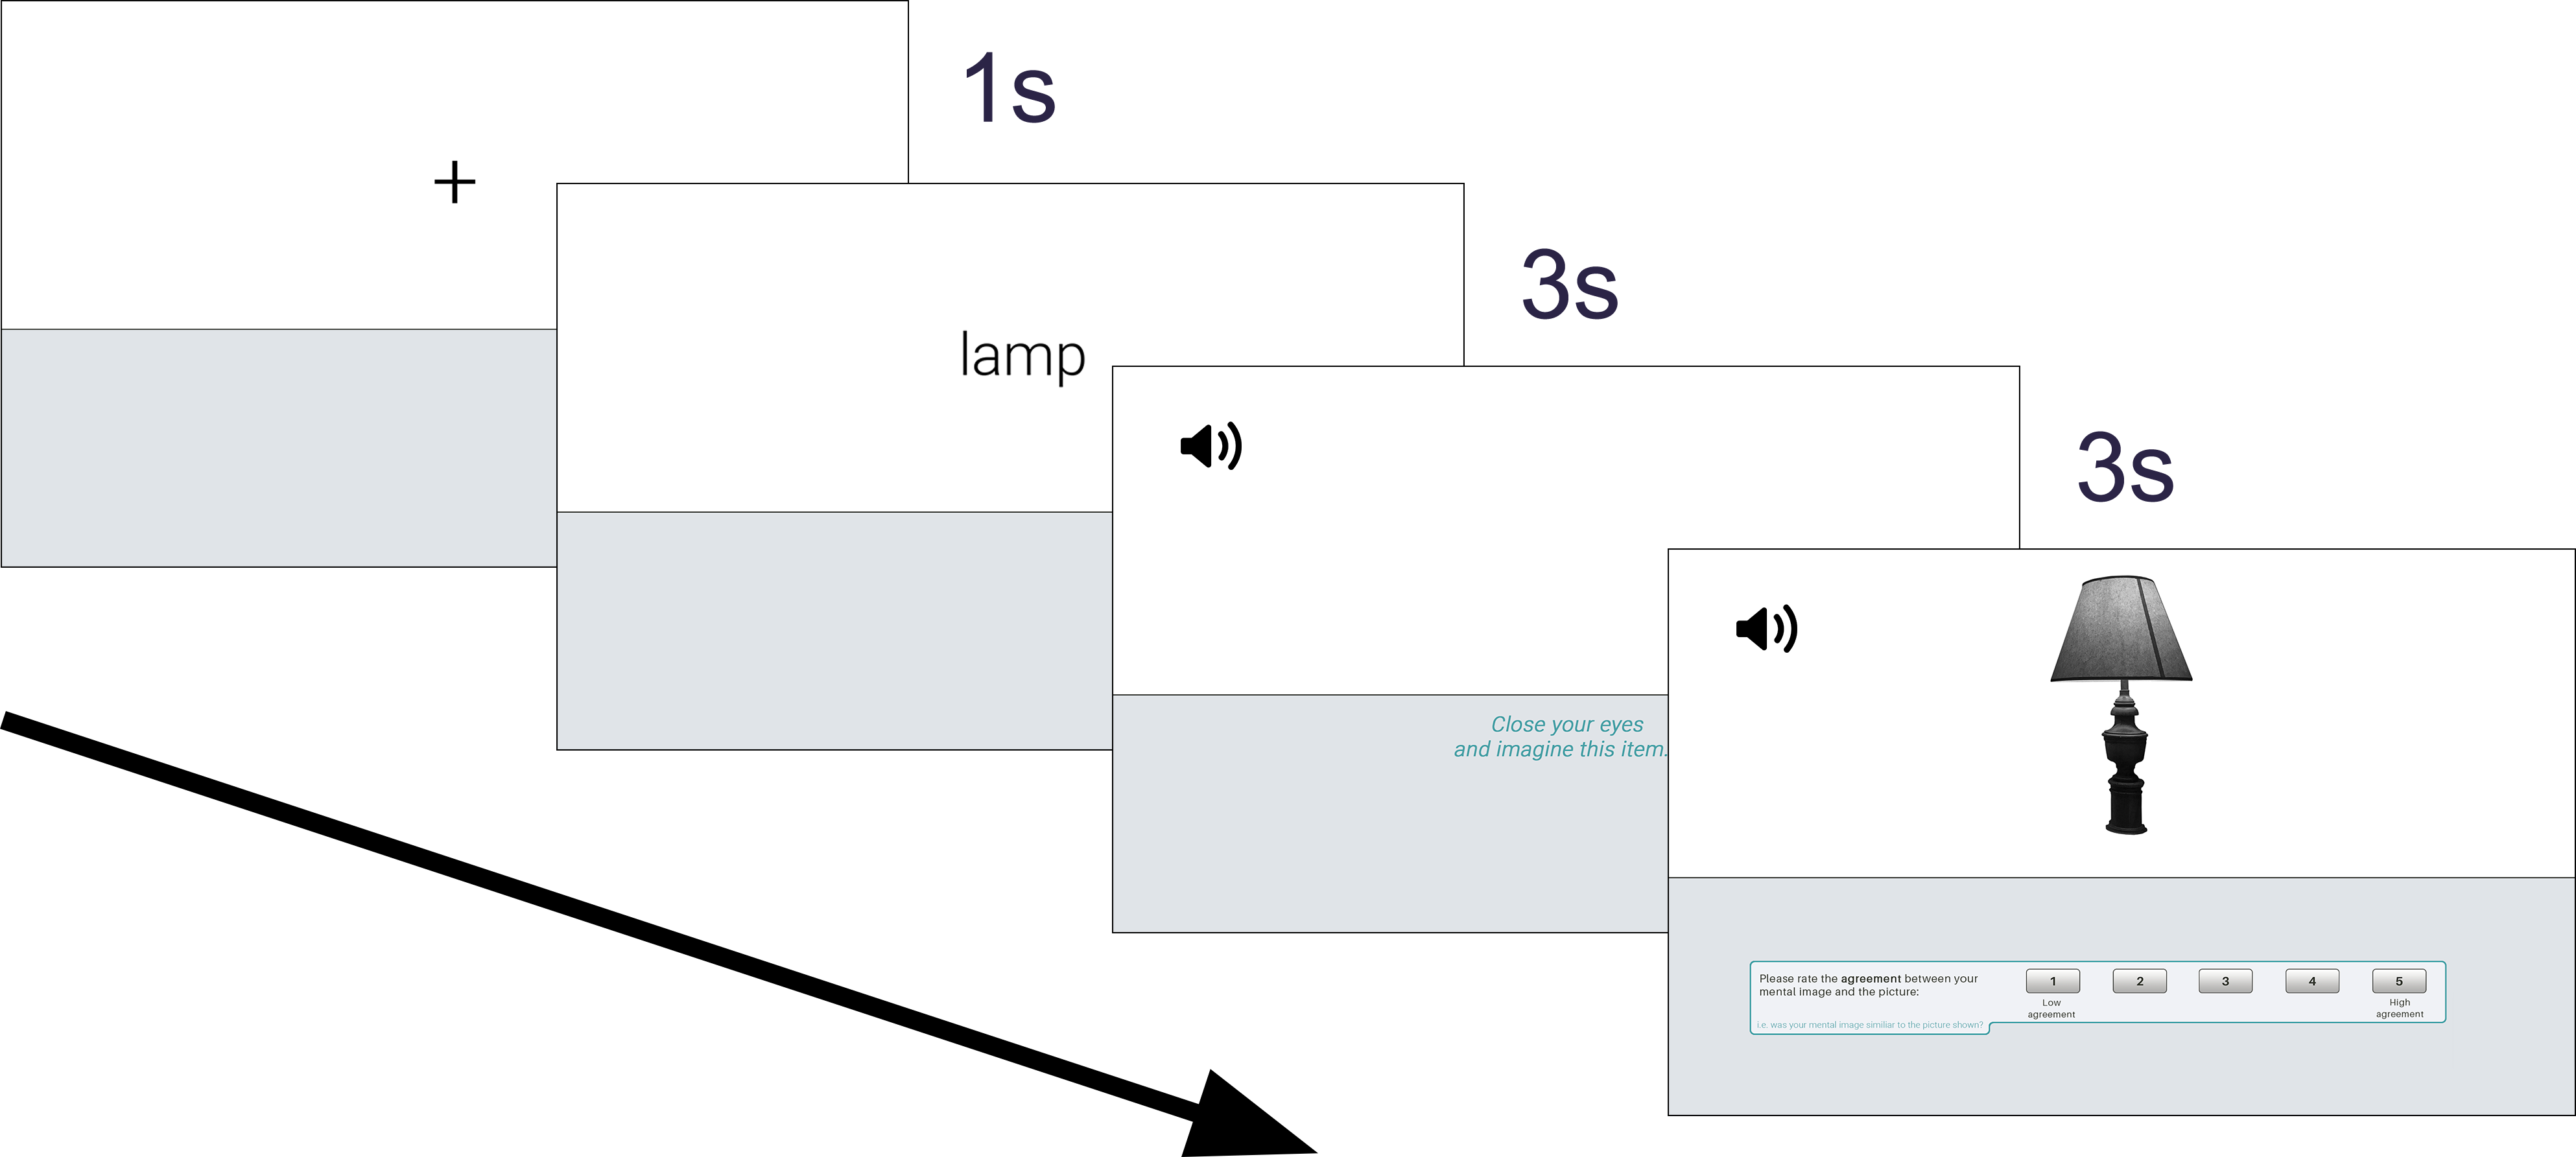
\includegraphics[width=1\linewidth]{./resources/images/procedure} ~ ~
Figure 10: Data collection procedure for Mental Imagery Agreement
responses. ~ ~

\hypertarget{data-processing-1}{%
\paragraph{Data processing}\label{data-processing-1}}

The naming responses for each photograph item were manually assessed for
spelling and typing errors. Automatic spell checking software was
avoided in an effort to avoid inadvertently introducing unique names
that were not actually given by participants. The vast majority of
errors were unambiguous and easy to correct (e.g.~``anker'' =
``anchor'', ``peguin'' = ``penguin'', ``ssnowman'' = ``snowman''), or
consisted of transforming plural words to singular (or vice versa,
depending on the form of the intended label - e.g.~``sock'' to
``socks''). Some responses were a little more ambiguous, and
necessitated comparison to the photographs they were in response to for
additional clarity (e.g.~a photograph depicting a plug that would fit
into North American electrical sockets was labelled as ``usplug'' -
given the nature of our UK-based sample, it's likely the subject was
responding: ``U.S. (i.e.~United States) plug''.

There were instances where subjects provided a sensible and correctly
spelled English word, but that were clearly typos when examined against
the photograph they were in response to (e.g.~``dock'' for a photograph
depicting a duck, ``frock'' for a frog, and ``beer'' for a ``bear'',
etc). The most ambiguous spelling error to correct was ``bittle'', which
was provided by more than one participant and to more than one item;
separate inspections of the photographs participants were responding to
made this easy to correct though, with one participant clearly meaning
to respond ``bottle'', whilst the other meant to respond ``beetle''.
Though participants were instructed to only give a single label for each
item, some multiple word responses were found (without spaces) during
the spell checking process. On such occasions, a judgement was made
regarding whether multiple words were retained, or whether the response
could be shortened into a single word. A general rule was applied
whereby if the other words provided additional information, they were
retained (e.g.``maledear'' - presumably ``male deer'' - was kept as a
two-word answer). Multiple word responses were generally shortened into
a single word when the intended label for the item was clearly present,
and no information was lost in the process (e.g.~``haircomb'' was
shortened to the intended answer ``comb''). It is noted that there was
some inherent subjectivity in this process, though as such items were
not common among straightforward responses, their overall effects are
estimated to be negligible.

Finally, there were some responses that were changed to ``no'' as they
were clearly intended to signify that the responder did not know the
name of the item shown; the experiment instructed participants to type
``no'' in these instances, though the labels ``none'' and ``idk''
(common abbreviation for ``I don't know) were provided instead. There
was also a single response that was manually changed to''no``, as the
provided label was a single letter and thus entirely unclear what the
intended answer should be (see Appendix A for full list of manipulations
to naming responses). This process yielded data that could be used to
determine which photograph variation best matched the intended concepts
(e.g.~100\% of participants labelled the object ``bottle'', indicating a
perfect match), and which did not (e.g.~only 50\% of participants
labelled the item ``bottle'', whilst the other 50\% gave the label
``wine'', indicating a poor match). Photographs showing poor agreement
across participant-generated labels, or those where the majority of
labels differed from the intended concept, could be replaced with the
variation demonstrating the most accurate depiction.

\hypertarget{analysis-preperation}{%
\paragraph{Analysis preperation}\label{analysis-preperation}}

A number of variables were calculated prior to analysis. For
familiarity, visual complexity, colour diagnosticity, and mental imagery
agreement, mean ratings were calculated for each (see Appendix B). Mean
reaction times (RTs) were also calculated for each photograph / response
variable, including naming responses. For naming responses, accuracy was
defined as the proportion of subjects reporting the correct/intended
label for any given item (e.g.~80\% of subjects correctly labelled a
photograph of the moon as ``moon''). Percentage agreement was also
calculated (i.e.~the proportion of subjects providing the most frequent
name, regardless of whether it matched the correct/intended label) in
order to compute \emph{H} values for each item. The \emph{H} statistic
also reflects naming agreement, but it takes into account the total
number of unique labels given for an item. This is especially useful for
comparing similar items, as it captures information not provided by
simple agreement proportions. For instance, if the first variation of
the photo moon (`moon-1') demonstrated 90\% naming agreement among
subjects, and the second variation (`moon-2') also demonstrated 90\%
naming agreement, it would appear as if both versions offer the same
level of agreement among participants. However, `moon-1' may have
received a total of 2 unique names (e.g.~moon, planet), while `moon-2'
received a total of 4 unique names (e.g.~moon, planet, earth, comet).
\emph{H} values utilise this useful information to determine which item
shows the best naming agreement (in other words, the item with the least
number of unique names). The original formula by Snodgrass \& Vanderwart
(1980) was used to calculate \emph{H} values:

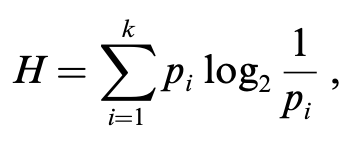
\includegraphics[width=0.5\linewidth]{./resources/images/h_calculation}

A \emph{H} value of 0 indicates perfect naming agreement (all subjects
responded with the same label for that item). Items showing a \emph{H}
value of 1 signify two unique names were provided, with identical
proportions (e.g.~10 subjects responded ``moon'' and 10 subjects
responded ``planet''). As the \emph{H} value increases, overall naming
agreement decreases.

\hypertarget{results-1}{%
\subsubsection{Results}\label{results-1}}

Summary statistics (mean and \emph{SD}) for each of the measured
variables are shown in Table 4. Data for the grey and colour photographs
are presented alongside previously obtained normative values for a
number of other stimuli formats (all obtained from Rossion \& Pourtois
(2004), who published revised norms for Snodgrass \& Vanderwart (1980)'s
(S\&V) original line drawings, as well as their own re-drawn versions
that contained shading and texture detail). The data from previous
studies were not used in any statistical analyses. To examine whether
the grey and colour photographs from the current study demonstrated any
differences, a series of independent samples t-tests were run on each
variable, as well as their corresponding reaction times (excluding
scores of colour diagnosticity, which were obtained only in response to
the colour items and thus cannot be compared). Mean (and \emph{SD})
values for all x816 unique photograph items are presented in Appendix B.

\hypertarget{naming}{%
\paragraph{\texorpdfstring{\emph{Naming}}{Naming}}\label{naming}}

Naming accuracy was very high for all photographs (\emph{M} = 0.95),
indicating that overall, the selected items closely depicted the
intended concepts. Compared with the other stimuli formats, there
appears to be a steady increase in accuracy as items become more
distinctive (see Table 4). Accuracy rates did not differ between the
grey (\emph{M} = 0.94) and colour (\emph{M} = 0.95) versions of the
photographs {[}\(t(745.64) = -0.56\), \(p = .576\){]}.

\emph{H} values were also low across all items (\emph{M} = 0.23),
showing that subjects generally agreed on how the items should be named.
Similar to naming accuracy, naming agreement also appears to steadily
increase as items become more distinctive (as indicated by decreasing H
values - see Table 4. While Rossion \& Pourtois (2004) observed
significantly better naming agreement for their colour - rather than
greyscale - items, this pattern did not reach significance with the
current set of photographs; \emph{H} values did not differ between the
grey (\emph{M} = 0.24) and colour (\emph{M} = 0.22) photographs
{[}\(t(743.66) = 0.62\), \(p = .537\){]}.

A mean reaction time (RT) of (3.9s) was observed for naming responses.
While this was of little interest on its own, and could not be compared
to those obtained in response to the other stimuli formats as our
methodology was slightly different (RTs were only recorded when subjects
had typed their response \emph{and} clicked the mouse to signify they
had finished), they were useful for marking comparisons between the grey
and colour items (though no difference was observed {[}\emph{M} grey =
4s, \emph{M} colour = 3.8s, \(t(651.86) = 1.57\), \(p = .117\){]}).
Overall, these analyses suggest that the current photographs closely
resemble the drawings they were designed to match, with high levels of
naming accuracy and agreement among subjects. The absence of any colour
differences indicates there were no naming advantages when photographs
were made even more distinctive through the addition of colour.

Table 4: Summary statistics for each of the measured variables. Mean
values are presented in bold (SDs are shown in parentheses).

\begin{table}[!h]
\centering
\begin{tabular}{>{\raggedright\arraybackslash}p{13em}>{\centering\arraybackslash}p{3.8em}>{\centering\arraybackslash}p{3.8em}>{\centering\arraybackslash}p{3.8em}>{\centering\arraybackslash}p{2em}>{\centering\arraybackslash}p{3.8em}>{\centering\arraybackslash}p{3.8em}}
\toprule
\multicolumn{1}{c}{ } & \multicolumn{3}{c}{Rossion \& Pourtois (2004)} & \multicolumn{1}{c}{ } & \multicolumn{2}{c}{Current study} \\
\cmidrule(l{3pt}r{3pt}){2-4} \cmidrule(l{3pt}r{3pt}){6-7}
  & S\&V lines & Grey shaded & Colour shaded &    & Grey photos & Colour photos\\
\midrule
\textbf{Naming accuracy} & \textbf{88.2} & \textbf{89.2} & \textbf{90.3} & \textbf{} & \textbf{0.94} & \textbf{0.95}\\
\em{} & \em{(17.1)} & \em{(17.2)} & \em{(16.9)} & \em{} & \em{(0.08)} & \em{(0.08)}\\
\textbf{Naming agreement (H)} & \textbf{0.44} & \textbf{0.38} & \textbf{0.32} & \textbf{} & \textbf{0.24} & \textbf{0.22}\\
\em{} & \em{(0.56)} & \em{(0.52)} & \em{(0.46)} & \em{} & \em{(0.33)} & \em{(0.31)}\\
 &  &  &  &  &  \vphantom{2} & \\
\addlinespace
\textbf{Mental imagery agreement} & \textbf{3.73} & \textbf{3.76} & \textbf{3.74} & \textbf{} & \textbf{3.46} & \textbf{3.74}\\
\em{} & \em{(0.48)} & \em{(0.55)} & \em{(0.63)} & \em{} & \em{(0.56)} & \em{(0.65)}\\
 &  &  &  &  &  \vphantom{1} & \\
\textbf{Familiarity} & \textbf{3.59} & \textbf{3.52} & \textbf{3.44} & \textbf{} & \textbf{4.13} & \textbf{4.19}\\
\em{} & \em{(0.94)} & \em{(1.01)} & \em{(1.01)} & \em{} & \em{(0.56)} & \em{(0.54)}\\
\addlinespace
 &  &  &  &  &  & \\
\textbf{Visual complexity} & \textbf{2.76} & \textbf{2.88} & \textbf{2.7} & \textbf{} & \textbf{2.87} & \textbf{3.16}\\
\em{} & \em{(1.03)} & \em{(1.03)} & \em{(0.94)} & \em{} & \em{(0.62)} & \em{(0.63)}\\
 & - & - & - &  & - & -\\
\textbf{Colour diagnosticity} & \textbf{-} & \textbf{-} & \textbf{-} & \textbf{} & \textbf{-} & \textbf{3.22}\\
\addlinespace
\em{} & \em{-} & \em{-} & \em{-} & \em{} & \em{-} & \em{(0.84)}\\
\bottomrule
\end{tabular}
\end{table}

\hypertarget{mental-imagery-agreement}{%
\paragraph{\texorpdfstring{\emph{Mental imagery
agreement}}{Mental imagery agreement}}\label{mental-imagery-agreement}}

Scores of mental imagery agreement were moderate across all items
(\emph{M} = 3.6). While no colour differences were previously observed
between stimuli formats, the grey (\emph{M} = 3.46) photographs in the
current study showed significantly lower mental imagery agreement scores
than the colour (\emph{M} = 3.74) items {[}\(t(800.06) = -6.54\),
\(p < .001\){]}. Comparisons with previous normative data also highlight
how the grey photographs exhibited uniquely poorer mental imagery
agreement scores than any of the other stimuli formats (see Table 4).
RTs between the grey (\emph{M} = 3.04) and colour (\emph{M} = 2.81)
items did not significantly differ {[}\(t(571.37) = 2.14\),
\(p = .033\){]}.

\hypertarget{familiarity}{%
\paragraph{\texorpdfstring{\emph{Familiarity}}{Familiarity}}\label{familiarity}}

Familiarity scores were high overall (\emph{M} = 4.16), and like
previous findings, there was no difference between the grey (\emph{M} =
4.13) and colour (\emph{M} = 4.19) items {[}\(t(813.19) = -1.63\),
\(p = .103\){]}. However, familiarity scores for the current set of
photographs were higher than those obtained for any of the other stimuli
formats, and while there previously appeared to be a decline in
familiarity as stimuli become more distinctive (from line drawings, to
grey shaded, to colour shaded), such a pattern was not evident with the
current photographs (see Table 4). RTs between the grey (\emph{M} =
0.97) and colour (\emph{M} = 0.98) items did not significantly differ
{[}\(t(783.66) = -0.30\), \(p = .762\){]}.

\hypertarget{visual-complexity}{%
\paragraph{\texorpdfstring{\emph{Visual
complexity}}{Visual complexity}}\label{visual-complexity}}

Visual complexity ratings were moderate across all of the items
(\emph{M} = 3.3). Colour (\emph{M} = 3.16) photographs showed
significantly higher scores of visual complexity than grey (\emph{M} =
2.87) photographs {[}\(t(813.51) = -6.65\), \(p < .001\){]}. This
finding is further demonstrated when compared to the scores from the
other stimuli formats (see Table 4); where grey photographs show
comparable levels of visual complexity, the colour photographs show
higher scores than all of the other formats. There was no significant
difference between the RTs of grey (\emph{M} = 3.26) and colour
(\emph{M} = 3.35) items {[}\(t(754.08) = -1.21\), \(p = .228\){]}.

\hypertarget{selection-of-final-items}{%
\paragraph{\texorpdfstring{\emph{Selection of final
items}}{Selection of final items}}\label{selection-of-final-items}}

For each concept represented in the photographs, one variation
(e.g.~shoe-1, shoe-2, or shoe-3) was selected for inclusion in a final
list of stimuli that would be taken forward into subsequent recognition
experiments. The normative naming data was assessed to establish which
version best matched the existing line-drawn depictions of the concepts
(Rossion \& Pourtois, 2004). Naming was favoured over all of the other
variables as, if an item was found to primarily convey a different
concept than was intended during the naming task (e.g.~if a photograph
of the fruit `orange' was labelled `grapefruit' by the majority of
subjects), then it could not be sufficiently compared to its line-drawn
(and written-word) counterpart during recognition studies.

At least 20 unique naming responses were collected for each of the 816
photographs (408 grey items and 408 colour items). The proportion of
`correct' responses (i.e.~names that were congruent with the intended
concept) and the proportion of `don't know' responses were calculated
for each item. Photographs were excluded if they:

\begin{enumerate}
\def\labelenumi{\arabic{enumi}.}
\tightlist
\item
  received a high proportion of ``don't know'' responses (20\%; all of
  the photographs depicted common, everyday objects, and so if a number
  of subjects were unable to name the item, that particular photograph
  was considered to be a poor representation of the item);
\item
  were incorrectly named by the majority of subjects (i.e.~if the
  proportion of correct responses equalled ≤ 50\%, since it was
  essential for the photographs to depict the same concepts as those
  found in the shaded drawings and word stimuli);
\item
  had particularly poor naming agreement (≤ 20\% subjects named the
  object similarly). Items may not have been flagged by the second
  criteria (e.g.~if it received 4 different names, each with a 25\%
  ratio), but could still be considered poor representations of the
  intended concepts.
\end{enumerate}

54 photographs were found to meet at least one of the above criteria,
and therefore excluded. Regardless of whether these items were grey or
colour, it was also necessary to remove its grey or colour partner
(since both versions were needed to make comparisons across recognition
experiments). Thus, a total of 64 items (32 grey / 32 colour) were
excluded at this stage (many items already had both grey and colour
versions flagged by the original criteria).

Next, the proportion of correct responses were compared between grey and
colour photographs in order to identify items showing the lowest
difference. In order to manipulate colour in later recognition
experiments, it was important to select items where naming was congruent
across colour/grey items; in other words, it would be difficult to
attribute particular recognition response patterns to the addition of
colour (if a difference were found) when the grey version could not be
identified (or encoded) similarly. Variations exhibiting the least
difference between colour and grey items (for the proportion of correct
responses) were taken forward, while the rest were excluded. In a number
of instances, multiple variations for the same object had the same
`difference' score. For example, all three variations of the item
``balloon'' exhibited perfect naming agreement, irrespective of whether
they were presented in colour or grey (and thus ``balloon1'',
``balloon2'', and ``balloon3'' had a difference score of 0). For items
where more than 1 variation remained, manual rankings were obtained from
two of the researchers to determine which variation best depicted the
intended concept. For each item, the researchers independently studied
the remaining variations and provided a rank of which they thought was
best (1) to worst (2 or 3, depending on the number of variations that
remained). The ratings from both researchers were collated; items where
there was agreement as to which variation best depicted the intended
concept were selected for inclusion in the final stimuli list. For all
the items where there was disagreement between the researchers rankings,
one of the variations was simply selected at random.

\hypertarget{discussion-1}{%
\subsubsection{Discussion}\label{discussion-1}}

\hypertarget{the-role-of-colour}{%
\paragraph{\texorpdfstring{\emph{The role of
colour}}{The role of colour}}\label{the-role-of-colour}}

For naming responses (accuracy, agreement {[}\emph{H}{]}, and RTs), no
differences were observed between the grey and colour photographs. Such
a result was expected for accuracy and agreement scores; the
addition/absence of colour should not alter how participants identify
(and thus label) items, except in rare instances whereby a lack of
colour may lead to the misidentification of an object (e.g.~incorrectly
labelling a greyscale photograph of an orange as `grapefruit'). The data
indicates, however, that this was not common, with the grey set of
photographs exhibiting equally high levels of naming accuracy as the
colour photographs. The absence of RT differences between the colour and
greyscale sets was not expected for naming responses. It is reasonable
to assume that colour photographs - with an additional layer of
contextual information compared to grey items - would be identified (and
therefore named) quicker than grey photographs (e.g.~a colour photograph
of an orange should avoid the potential ambiguity that might accompany a
greyscale depiction, which could initially be confused for another type
of fruit). Indeed, Rossion \& Pourtois (2004) demonstrated RTs
consistent with this hypotheses, with colour drawings showing
significantly quicker RTs than grey items. The lack of difference in the
current data could be attributable to ceiling effects, whereby all
photographs were sufficiently unambiguous, and were quickly identified
irrespective of whether they were presented in greyscale or colour.
Examination of the other naming data, showing similarly high levels of
accuracy and agreement across grey and colour, supports this notion.

Scores of mental imagery agreement produced particularly interesting
results between the grey and colour items. Grey photographs exhibited a
significantly poorer match with subjects imagined presentation of the
objects than the colour items. Colour differences were not observed
previously between drawings (Rossion \& Pourtois, 2004), and comparing
the current data with that obtained in other studies (see Table 4)
demonstrates how the greyscale photographs show uniquely lower mental
imagery agreement scores compared with any of the other stimuli formats.
To imagine the objects, it seems likely that subjects would conjure an
image of how they naturally see the item in their everyday lives - which
for the majority of subjects, would presumably be a colour
representation. Therefore, when presented with greyscale depictions,
subjects may have been more inclined to report that that item did not
align quite as well as those presented in colour. However, it is unclear
why a similar pattern is not also evident when comparing grey and colour
drawings (Rossion \& Pourtois, 2004). It may be that photographs promote
stricter internal criteria when subjects must decide whether an item is
a good match to their mental image. With line-drawn / illustrated items,
subjects may simply accept that the items are baseline depictions, and
that they will only able to match their real-world mental images to a
certain degree - thus leading to a generally more liberal response bias
throughout. The addition of colour may therefore do very little to
further reconcile the match between the drawing and real-world mental
representation. When subjects are responding only to photographs, the
ecological nature of the items may facilitate deeper critical evaluation
of whether they offer a good match to mental images, and thus promote a
more conservative response bias. Colour may therefore be a far more
important factor in photographs than it is in drawings for allowing
participants to decide whether an item matches well with their mental
image.

There were no colour differences in familiarity scores. This result was
expected - participants were asked to rate the degree to which they came
in contact with, or think about, the concept itself rather than the
particular depiction shown, and there is no apparent reason why colour
should influence such ratings. Visual complexity, on the other hand,
where participants were required to directly rate the amount of detail
in the image, did show an expected difference. Colour photographs were
rated as significantly more visually complex than grey items, presumably
due to their additional layer of contextual information. When compared
to the previous data obtained for drawings, the greyscale photographs
showed comparable levels of visual complexity, while the colour
photographs showed higher levels than any of the other formats. It is
unclear why the photographs of the current study showed colour
differences, when grey and colour drawings did not differ, though it may
tie in with the hypotheses proposed to explain the mental imagery
agreement data. Subjects may apply stricter internal criteria when
rating stimuli that are perceived as being closer to how they would be
experienced in real life - when viewing a colour photograph of a rabbit,
it is difficult to see how we could make the item any more visually
complex than it already is (at least in a 2D medium). It's probable that
subjects notice the absence of colour when viewing the greyscale items,
since they depict the items in a way that they are not usually seen, and
thus determine that these items could be made more complex if they were
shown in colour (and so give lower visual complexity ratings as a
result).

\hypertarget{establishing-a-new-set-of-stimuli}{%
\paragraph{\texorpdfstring{\emph{Establishing a new set of
stimuli}}{Establishing a new set of stimuli}}\label{establishing-a-new-set-of-stimuli}}

The objective of the current study was to establish a new set of
ecological photograph stimuli to be taken forward into subsequent
recognition memory experiments. Matching items with previously
established drawings (and words) would allow for the effects of
stimuli-format on recognition response patterns to be directly examined.
A range of normative data was collected for 816 unique photograph items.
These items may prove useful for a range of cognitive researchers that
wish to utilise a set of high quality and realistic object stimuli,
especially given the flexibility of items that can be filtered based on
colour, naming agreement, familiarity, etc. For the needs of the current
body of research, the naming data was used to determine which
photographs best matched the intended concepts among a number of
possible variations. This allowed for the systematic comparison of
recognition memory performance toward three distinct stimuli formats
(words, drawings, and photographs) in the following study, in an effort
to establish how stimuli of varying perceptual distinctiveness may
affect recognition response patterns. Such comparisons might help to
reconcile the inconsistencies present across recognition memory
research, such as those attempted to determine whether familiarity
processes are preserved in those with amnestic Mild Cognitive Impairment
(aMCI).

\hypertarget{experiment-effect-of-stimuli-format-greyscale-and-response-option-on-recognition-memory-judgements.}{%
\subsection{Experiment: Effect of stimuli format (greyscale) and
response option on recognition memory
judgements.}\label{experiment-effect-of-stimuli-format-greyscale-and-response-option-on-recognition-memory-judgements.}}

For the recognition memory experiment, everyday objects were presented
in three stimuli formats: i) words (written in simple, black ink); ii)
drawings (shaded line-drawn illustrations); and iii) photographs (detail
rich exemplars of the real world object). Rossion \& Pourtois (2004)
demonstrated that naming agreement could be improved by adding surface
texture and shading to the original Snodgrass \& Vanderwart (1980)
items; however, it is unclear how manipulations to distinctiveness
actually impact performance in recognition memory paradigms. As well as
general inconsistencies regarding the type of stimuli used in
recognition memory experiments, there is also much variability in the
response options available to participants when reporting their
recognition, for example: Remember/Know (Lombardi et al. (2016)),
Recollection/Familiarity (???), or Low/Med/High confidence (???). In the
current experiment, the availability of different response options when
reporting recognition will also be examined by randomly assigning
participants into a paradigm with three response options (Recollection /
Familiarity / Guessing) or four response options (RFG + Both).

Based on the results of Experiment 1, which compared recognition to for
words and drawings only, a number of hypotheses are proposed as to the
potential effects of adding a third stimuli format (highly distinctive
photograph stimuli). As stimuli become increasingly distinctive (from
words, to drawings, to photographs), it seems likely that the number of
hits (correctly recognised items) will increase, and the number of false
alarms (FAs) will decrease. RFG responses are expected to show a similar
pattern, with the most detailed stimuli showing the highest number of
hits assigned ``Recollection'', while the less detailed formats show
increasing levels of ``Familiarity'' and ``Guessing'' hits. Whilst we
expect the overall number of FAs to increase as stimuli become less
distinctive (i.e.~words will show the highest rate of FAs), there is no
reason to believe that these FAs will be biased toward any particular
RFG judgement across formats. It is also hypothesised that the rates of
reported Recollection and Familiarity will differ across response option
conditions (RFG / RFBG), though the direction of this difference is
currently unclear.

\hypertarget{method-2}{%
\subsubsection{Method}\label{method-2}}

\hypertarget{participants-2}{%
\paragraph{Participants}\label{participants-2}}

A total of 169 subjects completed the online experiment (see Table 5 for
a breakdown of the gender and age of the sample). To meet our YA
requirements, all participants were required to be between 18-59 years
of age (actual range: 18-58). As our experiment involved English word
stimuli, we also asked subjects whether English was their first
language; the vast majority (95.86\%) reported that English was indeed
their first language. Subjects were recruited from voluntary
participation websites such as
Prolific Academic\footnote{\url{https://www.prolific.co/}} (73.37\%),
where payment at the rate of £5/hr was given, and via the in-school
research participation system\footnote{\url{https://keelepsychology.sona-systems.com/}}
(15.38\%), where they received course participation credits. A small
number of participants were also recruited from
Psychological Research on the Net\footnote{\url{https://psych.hanover.edu/research/exponnet.html}}
(11.24\%). In order to detect a medium effect size of Cohen's \emph{f} =
0.25 with 80\% power (\emph{α} = .05, two-tailed), G\emph{Power
indicated that we would need 79 participants per group (}N* = 158) in a
3x2 mixed ANOVA.

Table 5: Gender and age (\emph{SD}) of the current sample.

\begin{table}[!h]
\centering
\begin{tabular}{l>{}rr>{}l}
\toprule
Gender & N & Age &  \\
\midrule
Female & \em{102} & 29.64 & \em{(10.22)}\\
Male & \em{63} & 30.98 & \em{(10.97)}\\
Questioning & \em{1} & 21.00 & \em{(0)}\\
Unspecified & \em{3} & 50.33 & \em{(4.93)}\\
\textbf{Total} & \textbf{\em{169}} & \textbf{30.46} & \textbf{\em{(10.75)}}\\
\bottomrule
\end{tabular}
\end{table}

\hypertarget{materials-2}{%
\paragraph{Materials}\label{materials-2}}

A total of 126 innocuous, everyday objects (e.g.~clock, rabbit, shoe)
were presented across three individual stimuli formats: written words,
shaded drawings, and photographs. The drawings were obtained from
Rossion \& Pourtois (2004), and consisted of greyscale shaded
illustrations that contained some surface details. The word stimuli were
simply the written word names of the line-drawn objects, presented in a
clear Sans-serif typeface. The photograph stimuli were curated in the
previous study; high quality photographs were sourced to similarly
depict the same everyday objects as the shaded drawings. All objects in
the photographs were isolated from their original background, converted
to greyscale, and rotated to match the orientations shown in the
line-drawn items.

\hypertarget{design-2}{%
\paragraph{Design}\label{design-2}}

The current study utilised a mixed design, with a 3-level
within-subjects factor of stimuli format (words, drawings, photographs),
and a 2-level between-subjects factor of response option (RFG, RFBG).
Subjects passed through 2 levels of blocked randomization (equally
sized, predetermined blocks); first, participants were randomly assigned
one of six possible study lists (of equal length, and containing an even
number of word, drawing, and photograph items) for counterbalancing
purposes. Subjects were then either assigned into a recognition test
with three possible response options (RFG: ``Recollection'',
``Familiarity'',``Guessing''), or four possible response options (RFBG:
``Recollection'', ``Familiarity'', ``Guessing'', ``Both''). These
randomisation processes were completed automatically by the experiment
software using balanced methods.

~ ~

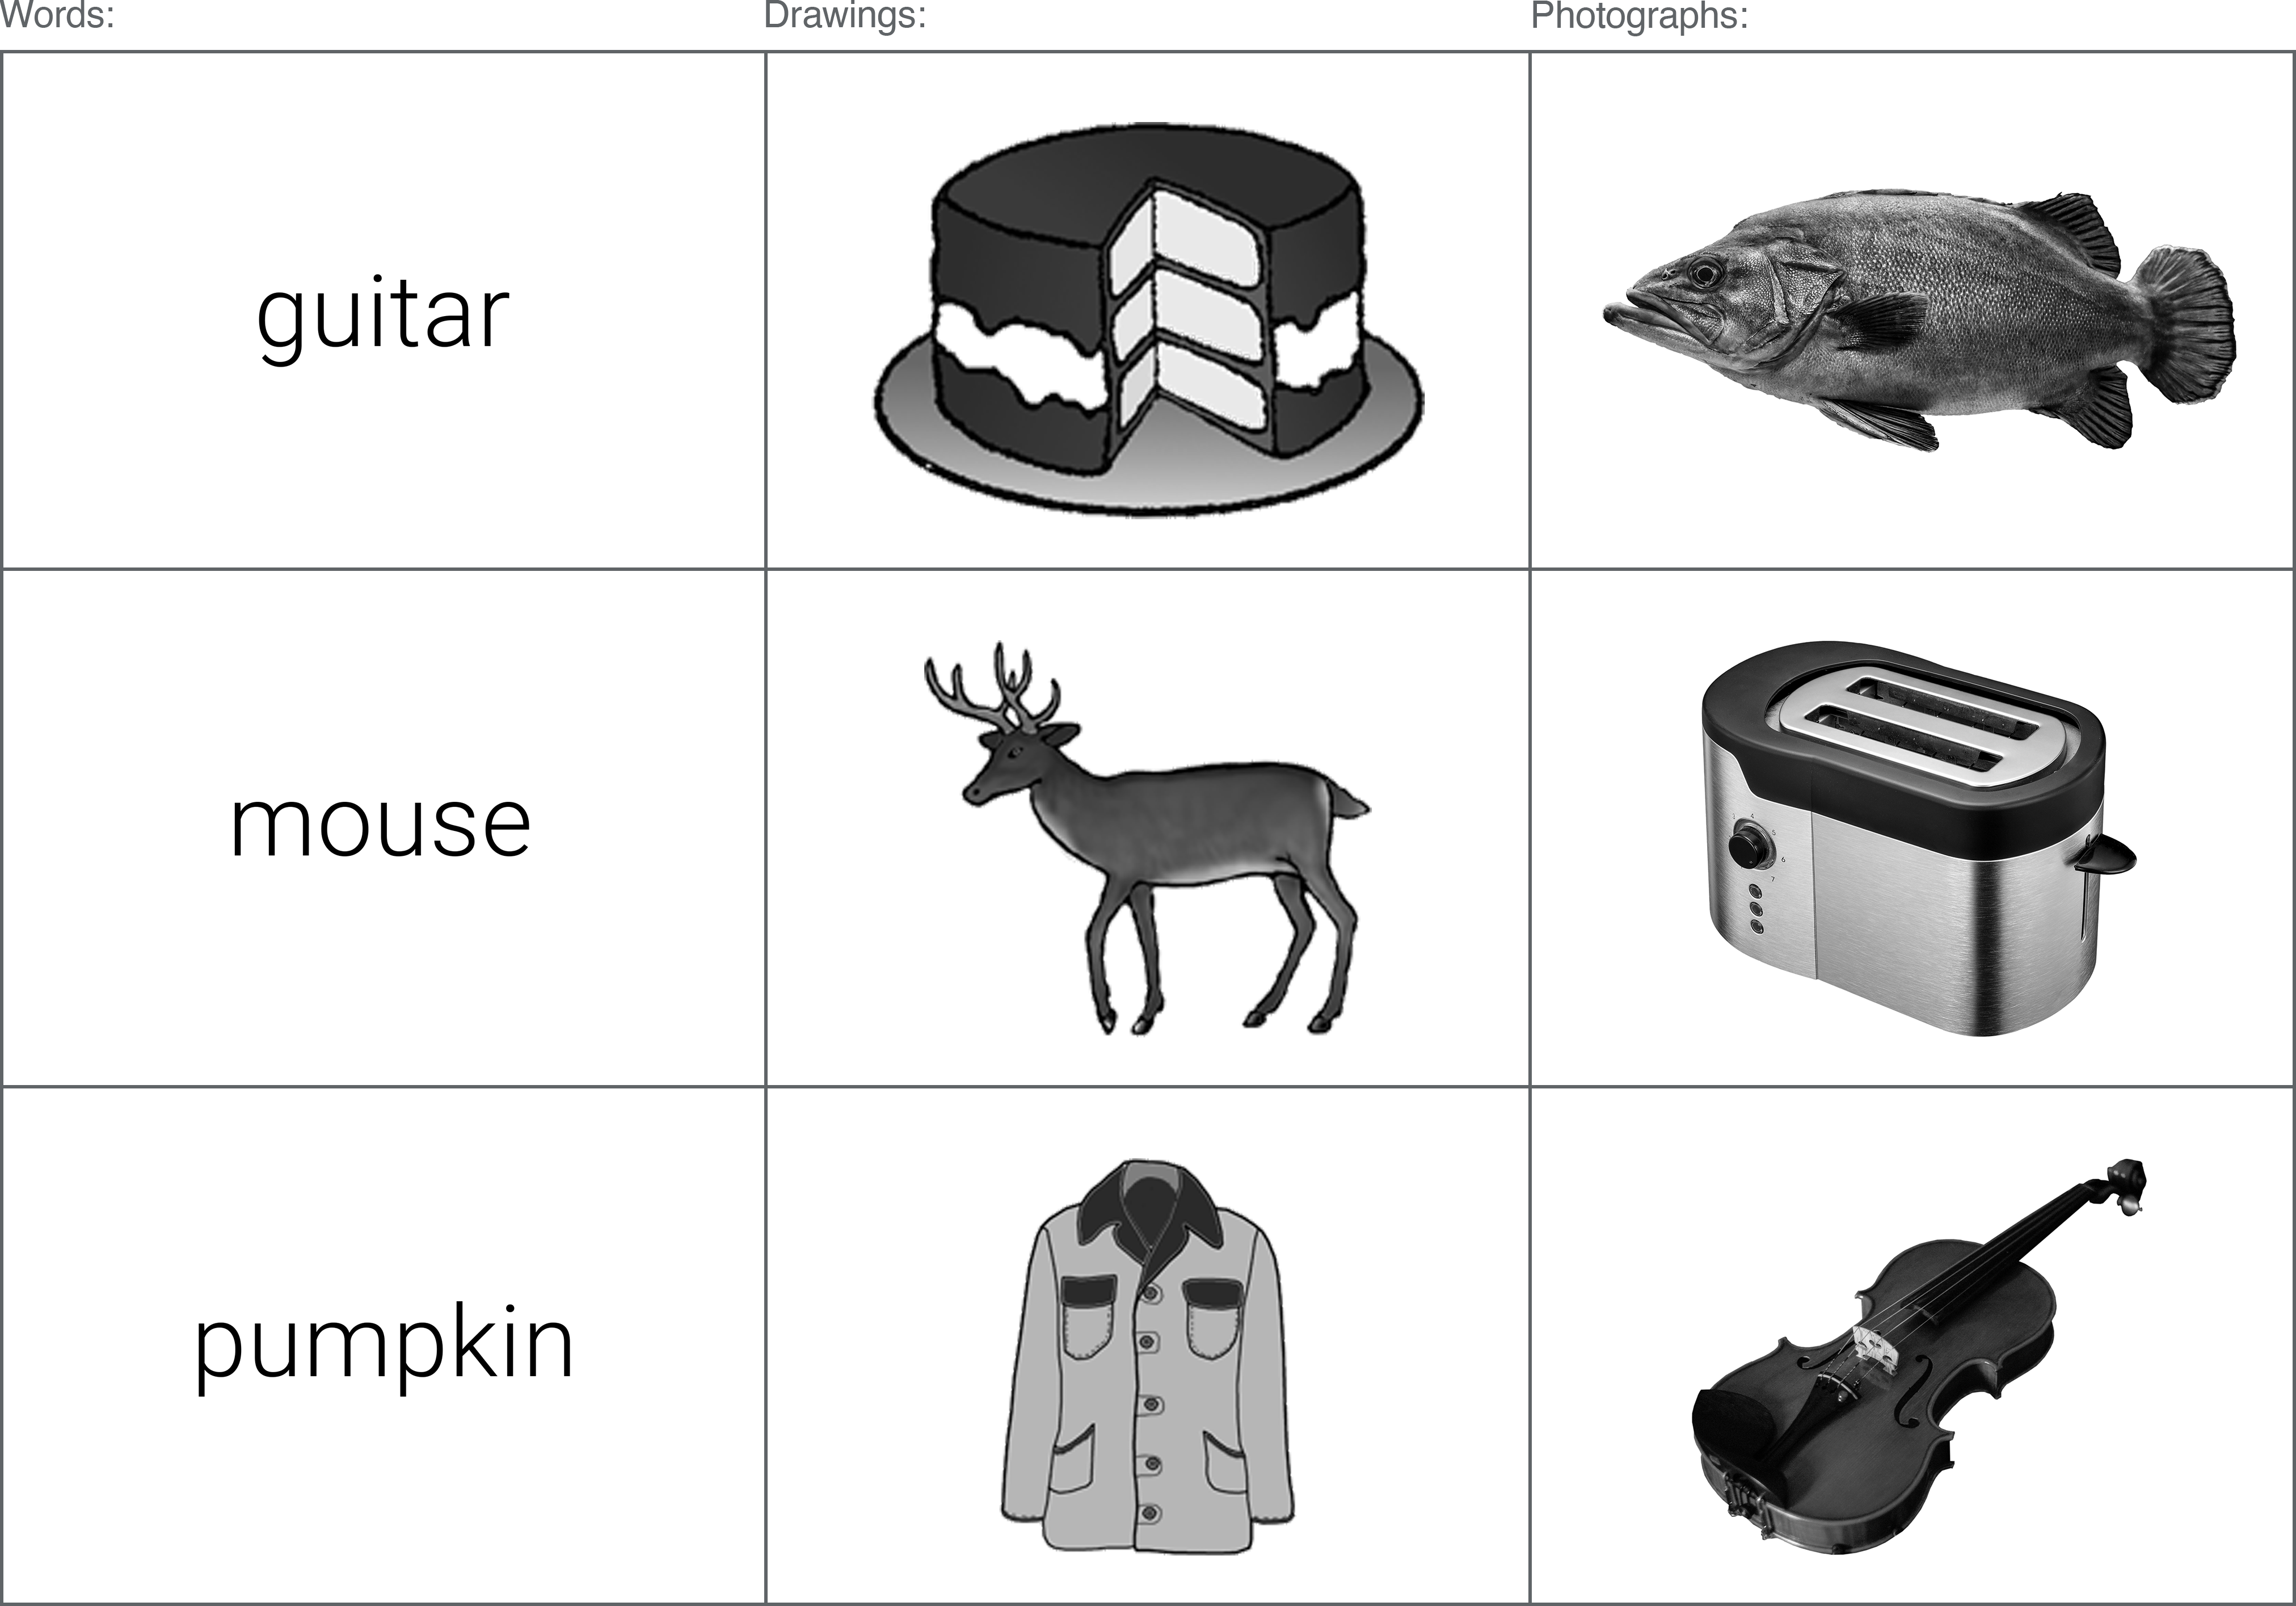
\includegraphics[width=1\linewidth]{./resources/images/exp3__stim_examples}
~ ~ Figure 11: Examples of the word, greyscale drawing, and greyscale
photograph stimuli utilised in the current experiment. ~ ~

\hypertarget{procedure-2}{%
\paragraph{Procedure}\label{procedure-2}}

Data was collected online using
Gorilla\footnote{\url{https://gorilla.sc/}} - a platform for the
building and hosting of online experiments. The experiment consisted of
three self-paced phases: i) study phase, ii) distractor task, and iii)
recognition test. In the study phase, an even mix of word, drawing, and
photograph stimuli were presented one-at-a-time on the computer screen.
Subjects were instructed to learn the items in preparation for a later
memory test. To ensure attention was directed to the presented stimuli,
subjects were required to report whether each item was shown as a word,
drawing, or photograph using the computer mouse. Following the study
phase, participants completed some simple multiple choice mathematical
questions (e.g.~6 x 4 = ?) as a distractor. Finally, participants memory
of the previously studied items was testing in the recognition task. An
even mix of word, drawing, and photograph stimuli were again presented
one-at-a-time on the screen; half of the test items had been shown
previously in the study phase, while the other half were new (and were
not on the study list). For each item, subjects were instructed to press
\emph{Old} if they believed it was an item they had studied earlier, and
\emph{New} if they had not. \emph{Old} responses led to a follow-up
judgement, where participants reported whether they had experienced
recognition through ``Recollection'', ``Familiarity'', or were simply
taking an uninformed ``Guess''. Participants that had been randomised
into the RFBG test condition had a fourth option here, whereby they
could report that they had experienced Recollection and Familiarity
simultaneously (``Both''). Stimuli format was congruent across the study
and test blocks (e.g.~items presented as photos at study were also
presented as photos at test). For each concept depicted across the three
stimuli formats, subjects were only presented with one variation (in
other words, if a subject saw a photograph for the item ``shoe'', they
did not see the word or line-drawn version of ``shoe'').

\hypertarget{data-processing-2}{%
\paragraph{Data processing}\label{data-processing-2}}

Measured variables included the total number of hits and FAs, and the
total number of hits and FAs assigned to each of the available response
options (R/F/G and R/F/B/G). In order to create a common dependant
variable, proportions were calculated from these variables slightly
differently depending on the response option group. In the RFG-judgement
group, simple proportions were created from the total number of R
responses and the total number of F responses. In the RFBG condition,
however, the proportion of Both responses was separately added to R
proportions and F proportions. Additional DVs included: i) d' (d-prime,
a signal detection measure of sensitivity); ii) c-value (a measure of
response bias); iii) overall accuracy (hits / (hits + FAs)); iv)
reaction times for all responses.

Participants were excluded from analysis if they showed poor performance
during the encoding task; the relative ease of reporting whether each
item was shown as a word, drawing, or photograph prompted a performance
cut off of 90\% accuracy. This allowed for some accidental clicks /
incorrect responses toward potentially ambiguous items, though subjects
scoring less than 90\% were excluded on the assumption they did not
dedicate their full attention to the task. Subjects with extreme
z-scores were also excluded from analysis; those presenting z-scores of
+/- 3 (for total hits, total FAs, or overall recognition {[}hits minus
FAs{]}) were considered outliers. These criteria resulted in the
exclusion of 8 datasets, leaving a total of 161 in analyses.

\hypertarget{results-2}{%
\subsubsection{Results}\label{results-2}}

A series of 3x2 mixed ANOVAs were conducted on each of the DVs, using a
within-subjects factor of stimuli format (words / grey drawings / grey
photos) and a between-subjects factor of response option (RFG / RFBG);
the Greenhouse-Geisser correction was applied when data was found to
violate the assumption of sphericity (assessed using Mauchlys test
statistic). Significant main effects of stimuli format (and interaction
effects) were assessed using Bonferroni-adjusted pairwise comparisons.
When no interaction effects were present, significant main effects of
response option were assessed via standard two sample t-tests (when
group variances were equal) or Welch two sample t-test (when variances
were not equal); variance was assessed using Levene's test.

\hypertarget{stimuli-distinctiveness}{%
\paragraph{Stimuli distinctiveness}\label{stimuli-distinctiveness}}

~ Table 6: Mean proportion of hits, FAs, and mean \emph{d'} scores, by
stimuli format and response option condition.

\begin{table}[!h]
\centering
\begin{tabular}{>{\raggedright\arraybackslash}p{4cm}rrr}
\toprule
  & Hits & FAs & d'\\
\midrule
\addlinespace[0.3em]
\multicolumn{4}{l}{\textbf{Stimuli format}}\\
\hspace{1em}Words & 0.54 & 0.21 & 1.15\\
\hspace{1em}Grey drawings & 0.76 & 0.09 & 2.38\\
\hspace{1em}Grey photographs & 0.85 & 0.05 & 3.08\\
\addlinespace[0.3em]
\multicolumn{4}{l}{\textbf{Response option}}\\
\hspace{1em}RFG & 0.74 & 0.13 & 2.25\\
\hspace{1em}RFBG & 0.69 & 0.11 & 2.16\\
\bottomrule
\end{tabular}
\end{table}

The mean proportion of hits and FAs, and mean \emph{d'} scores are
presented in Table 6. ANOVA results demonstrated a significant main
effect of stimuli format for the mean proportion of hits, \emph{F}(1.76,
280.25) = 225.67, \emph{p} \textless{} .001, \(\eta^2_p\) = .59. Paired
samples t-tests showed that grey photographs (\emph{M}= 0.85) produced a
significantly higher proportion of hits than both words (\emph{M}=
0.54), \emph{t}(160) = 18.56, \emph{p} \textless{} .001; \emph{d} =
1.46, 95\% CI {[}1.27, 1.7{]}, and grey drawings (\emph{M}= 0.76),
\emph{t}(160) = -8.04, \emph{p} \textless{} .001; \emph{d} = -0.63, 95\%
CI {[}-0.8, -0.47{]}. A significantly higher proportion of hits was also
evident for grey drawings (\emph{M}= 0.76) compared to words (\emph{M}=
0.54), \emph{t}(160) = 13.6, \emph{p} \textless{} .001; \emph{d} = 1.07,
95\% CI {[}0.88, 1.31{]}). There were no significant interaction effects
between stimuli format and response option condition, \emph{F}(1.76,
280.25) = 0.58, \emph{p} = .540, \(\eta^2_p\) \textless{} .01.

The ANOVA on the mean proportion of FAs also demonstrated a significant
main effect of stimuli format \emph{F}(1.43, 226.74) = 90.19, \emph{p}
\textless{} .001, \(\eta^2_p\) = .36. Grey photographs (\emph{M}= 0.05)
produced significantly fewer FAs in comparison to both words (\emph{M}=
0.21), \emph{t}(160) = -11.84, \emph{p} \textless{} .001; \emph{d} =
-0.93, 95\% CI {[}-1.08, -0.79{]}, and grey drawings (\emph{M}= 0.09),
\emph{t}(160) = 5.59, \emph{p} \textless{} .001; \emph{d} = 0.44, 95\%
CI {[}0.31, 0.59{]}). The grey drawings (\emph{M}= 0.09) also showed a
significantly lower proportion of FAs compared to words (\emph{M}=
0.21), \emph{t}(160) = -7.98, \emph{p} \textless{} .001; \emph{d} =
-0.63, 95\% CI {[}-0.8, -0.45{]}. There were no significant interaction
effects between stimuli format and response option condition,
\emph{F}(1.43, 226.74) = 1.17, \emph{p} = .299, \(\eta^2_p\) \textless{}
.01.

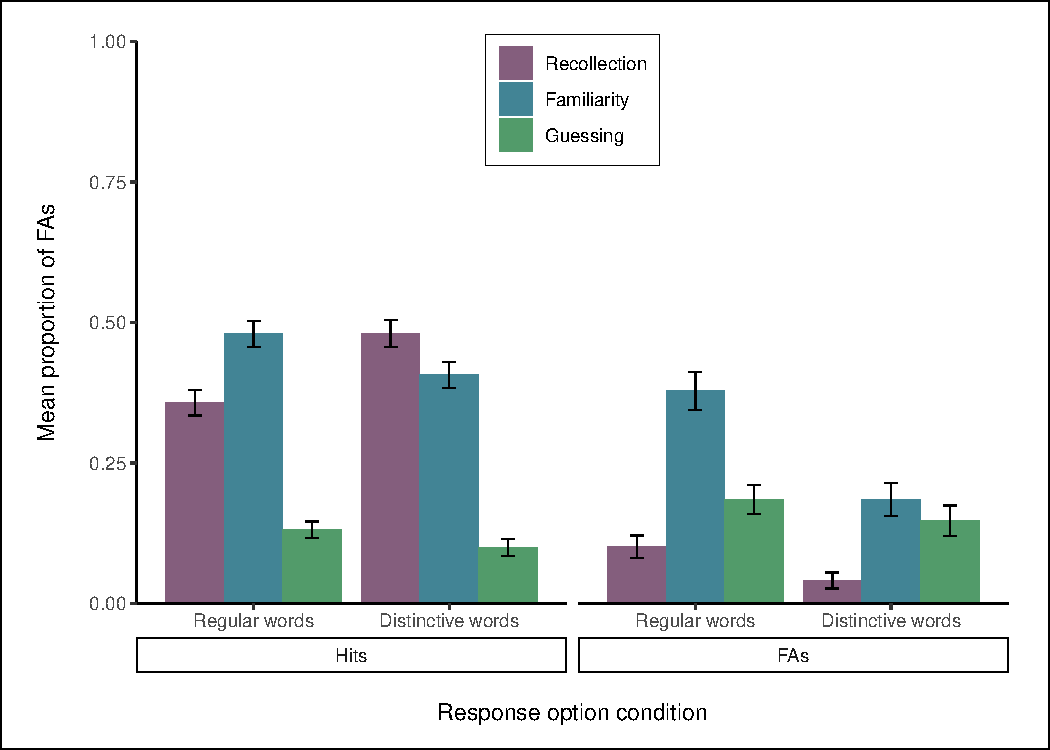
\includegraphics{R--Thesis_files/figure-latex/unnamed-chunk-41-1.pdf}
Figure 12: Interaction plot between stimuli format and response option
for d' scores. ~~

Results from the ANOVA on mean \emph{d'} scores showed a significant
interaction between stimuli format and response option condition,
\emph{F}(2, 318) = 3.34, \emph{p} = .037, \(\eta^2_p\) = .02 (see Figure
12). While \emph{d'} scores were numerically higher for words and grey
photographs in the RFG group (words \emph{M} = 1.25; grey photographs
\emph{M} = 3.19) compared to the RFBG group (words \emph{M} = 1.06; grey
photographs \emph{M} = 2.97), neither were significantly different from
one another (words: \emph{t}(320.69) = -1.38, \emph{p} \textgreater{}
.999; grey photographs: \emph{t}(320.69) = -1.54, \emph{p}
\textgreater{} .999. For grey drawings, however, this pattern was
reversed; \emph{d'} scores were numerically higher in the RFBG condition
(\emph{M} = 2.44) rather than the RFG condition (\emph{M} = 2.33);
though again, these means were not significantly different from one
another (grey drawings: \emph{t}(320.69) = 0.79, \emph{p} \textgreater{}
.999).

\hypertarget{recollection-and-familiarity}{%
\subparagraph{Recollection and
Familiarity}\label{recollection-and-familiarity}}

To determine the effects of stimuli format and response option on the
classification of recognition memory judgements, separate 3 (stimuli
format: words, drawings, photographs) x 2 (response option condition:
RFG-judgements, RFBG-judgements) mixed ANOVAs were conducted on the mean
proportion of hits assigned Recollection, Familiarity, and Guessing (see
Figure 13).

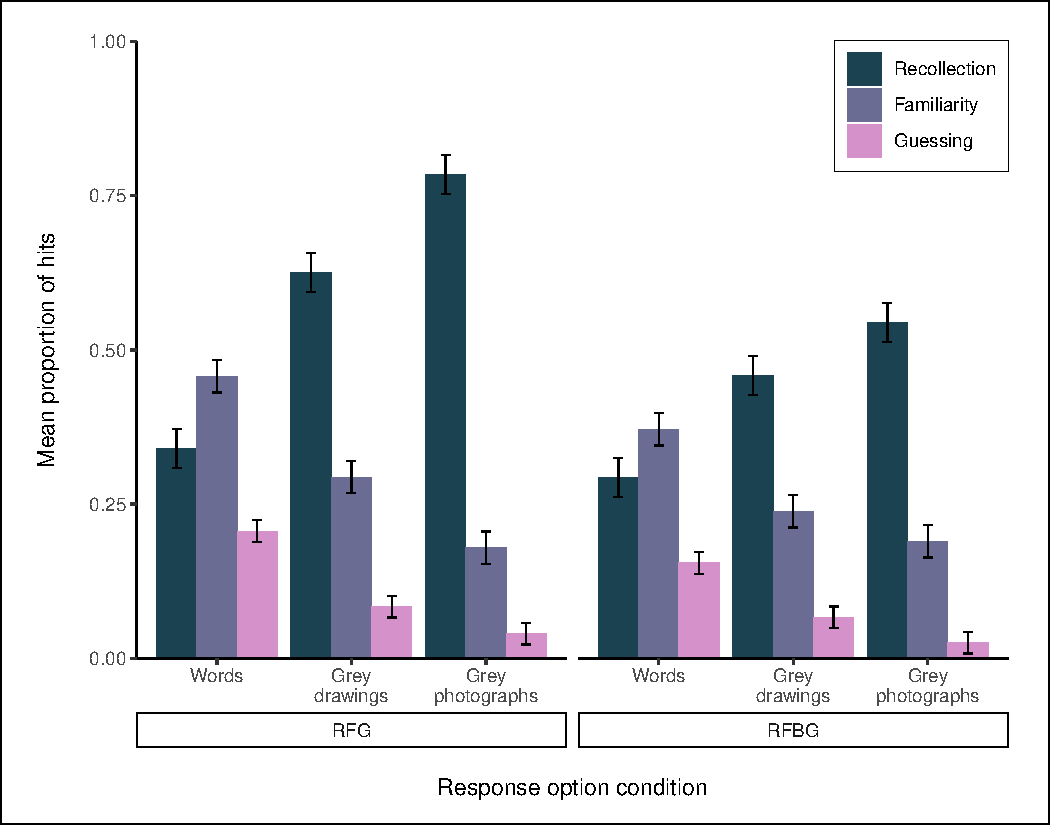
\includegraphics{R--Thesis_files/figure-latex/unnamed-chunk-43-1.pdf}
Figure 13: Proportion of hits assigned Recollection, Familiarity, and
Guessing, by stimuli format and response option condition.

Recollection (hits)

Results from the ANOVA on the mean proportion of hits assigned
Recollection showed a significant interaction between stimuli format and
response option condition, \emph{F}(1.74, 276.60) = 12.67, \emph{p}
\textless{} .001, \(\eta^2_p\) = .07 (see Figure 14).

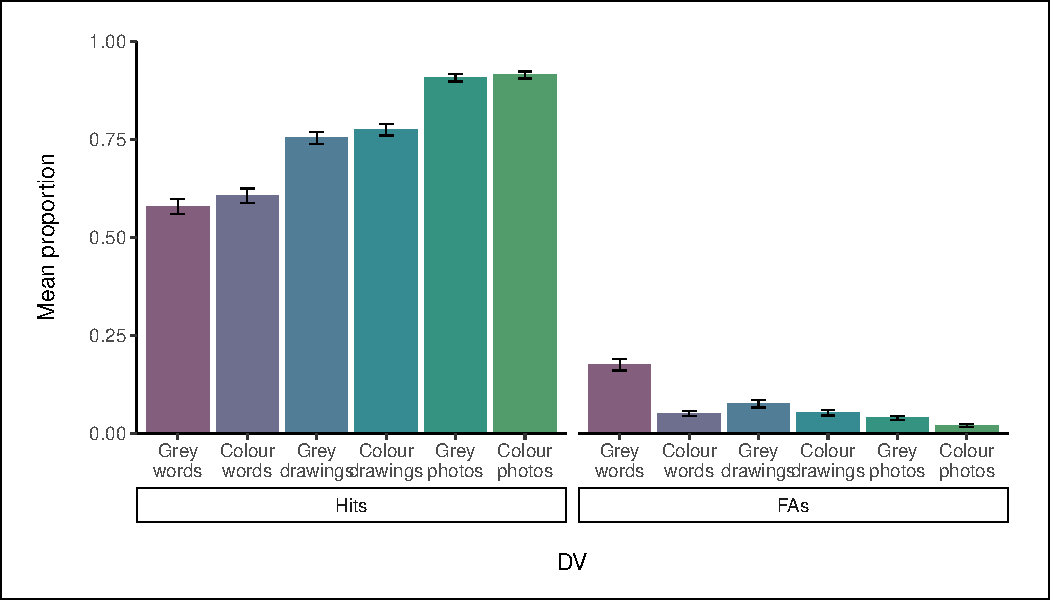
\includegraphics{R--Thesis_files/figure-latex/unnamed-chunk-45-1.pdf}
Figure 14: Interaction plot between stimuli format and response option
for the mean proportion of hits assigned Recollection. ~~

Comparisons across stimuli formats showed an expected pattern. Grey
photographs produced a significantly higher proportion of R hits than
words and grey drawings in both the RFG group (grey photographs
{[}\emph{M}= 0.78{]} vs.~words {[}\emph{M}= {]}, \emph{t}(318) = -16.46,
\emph{p} \textless{} .001; grey photographs {[}\emph{M}= 0.78{]}
vs.~grey drawings {[}\emph{M}= 0.63{]}, \emph{t}(318) = -5.87, \emph{p}
\textless{} .001) and the RFBG group (grey photographs {[}\emph{M}=
0.54{]} vs.~words {[}\emph{M}= {]}, \emph{t}(318) = -9.02, \emph{p}
\textless{} .001; grey photographs {[}\emph{M}= 0.54{]} vs.~grey
drawings {[}\emph{M}= 0.46{]}, \emph{t}(318) = -3.09, \emph{p} = .032).
Likewise, grey drawings produced a significantly higher proportion of R
hits in comparison to words in both the RFG (grey drawings {[}\emph{M}=
0.63{]} vs.~words {[}\emph{M}= {]}, \emph{t}(318) = -10.59, \emph{p}
\textless{} .001) and RFBG conditions (grey drawings {[}\emph{M}=
0.46{]} vs.~words {[}\emph{M}= {]}, \emph{t}(318) = -5.93, \emph{p}
\textless{} .001).

The interaction is evident following comparisons of the same stimuli
format across response option conditions. The RFG group produced a
significantly higher proportion of R hits than the RFBG group for grey
photographs (RFG {[}\emph{M} = 0.78{]} vs.~RFBG {[}\emph{M} = 0.54{]},
\emph{t}(266.67) = -5.33, \emph{p} \textless{} .001) and for grey
drawings (RFG {[}\emph{M} = 0.63{]} vs.~RFBG {[}\emph{M} = 0.46{]},
\emph{t}(266.67) = -3.72, \emph{p} = .004). However, this was not the
case for words, where there was no difference in the proportion of R
hits between the RFG (\emph{M} = ) and RFBG groups (\emph{M} = ;
\emph{t}(266.67) = -1.03, \emph{p} \textgreater{} .999).

Familiarity (hits)

Results from the ANOVA on the mean proportion of hits assigned
Familiarity showed a significant interaction between stimuli format and
response option condition, \emph{F}(1.61, 256.13) = 3.52, \emph{p} =
.041, \(\eta^2_p\) = .02 (see Figure 15).

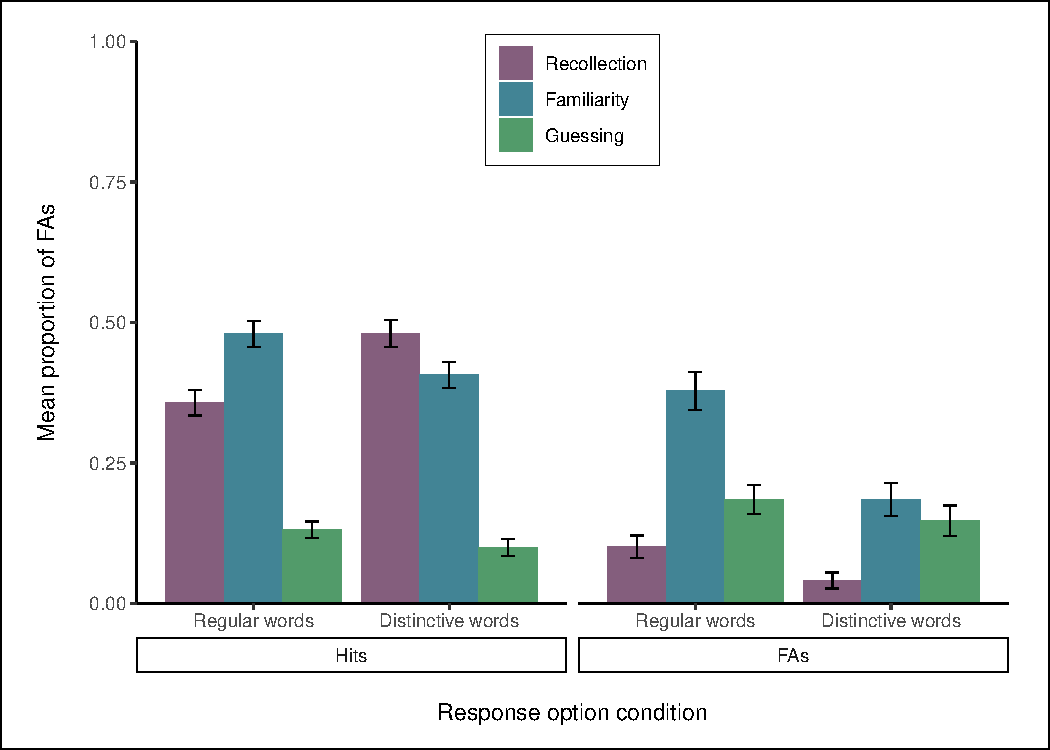
\includegraphics{R--Thesis_files/figure-latex/unnamed-chunk-47-1.pdf}
Figure 15: Interaction plot between stimuli format and response option
for the mean proportion of hits assigned Familiarity ~~

In the RFG group, grey photographs (\emph{M}= ) produced a significantly
lower proportion of F hits than both words (\emph{M}= ; \emph{t}(318) =
10.72, \emph{p} \textless{} .001) and grey drawings (\emph{M}= ;
\emph{t}(318) = 4.42, \emph{p} \textless{} .001). Grey drawings
(\emph{M}= ) in the RFG group similarly produced significantly fewer F
hits compared to words (\emph{M}= ; \emph{t}(318) = 6.30, \emph{p}
\textless{} .001). In the RFBG group, however, while grey photographs
(\emph{M}= ) again produced a significantly lower proportion of F hits
compared to words (\emph{M}= ; \emph{t}(318) = 6.77, \emph{p}
\textless{} .001), the difference in comparison to grey drawings
(\emph{M}= ) was no longer evident, \emph{t}(318) = 1.82, \emph{p}
\textgreater{} .999). Grey drawings (\emph{M}= ) in the RFBG group did
continue to produce significantly fewer F hits compared to words
(\emph{M}= ; \emph{t}(318) = 4.96, \emph{p} \textless{} .001).

Response option condition had no effect on the proportion of F hits
obtained, for either grey photographs (RFG {[}\emph{M} = {]} vs.~RFBG
{[}\emph{M} = {]}, \emph{t}(316.57) = 0.29, \emph{p} \textgreater{}
.999), grey drawings (RFG {[}\emph{M} = {]} vs.~RFBG {[}\emph{M} = {]},
\emph{t}(316.57) = -1.47, \emph{p} \textgreater{} .999), or words (RFG
{[}\emph{M} = {]} vs.~RFBG (\emph{M} = , \emph{t}(316.57) = -2.30,
\emph{p} = .336).

Guessing (hits)

The ANOVA on the mean proportion of hits assigned Guessing demonstrated
a significant main effect of stimuli format \emph{F}(1.33, 211.61) =
69.27, \emph{p} \textless{} .001, \(\eta^2_p\) = .30. Grey photographs
(\emph{M}= 0.03) produced significantly fewer G hits in comparison to
both words (\emph{M}= 0.18; \emph{t}(160) = -9.35, \emph{p} \textless{}
.001; \emph{d} = -0.74, 95\% CI {[}-0.87, -0.64{]}) and grey drawings
(\emph{M}= 0.08; \emph{t}(160) = 5.85, \emph{p} \textless{} .001;
\emph{d} = 0.46, 95\% CI {[}0.35, 0.59{]}). The grey drawings (\emph{M}=
0.08) also showed a significantly lower proportion of G hits compared to
words (\emph{M}= 0.18; \emph{t}(160) = -7.54, \emph{p} \textless{} .001;
\emph{d} = -0.59, 95\% CI {[}-0.73, -0.49{]}. There were no significant
interaction effects between stimuli format and response option condition
\emph{F}(1.33, 211.61) = 1.28, \emph{p} = .269, \(\eta^2_p\) \textless{}
.01.

To determine the effects of stimuli format and response option on the
classification of recognition memory judgements, separate 3 (stimuli
format: words, drawings, photographs) x 2 (response option condition:
RFG-judgements, RFBG-judgements) mixed ANOVAs were conducted on the mean
proportion of FAs assigned Recollection, Familiarity, and Guessing (see
Figure 16).

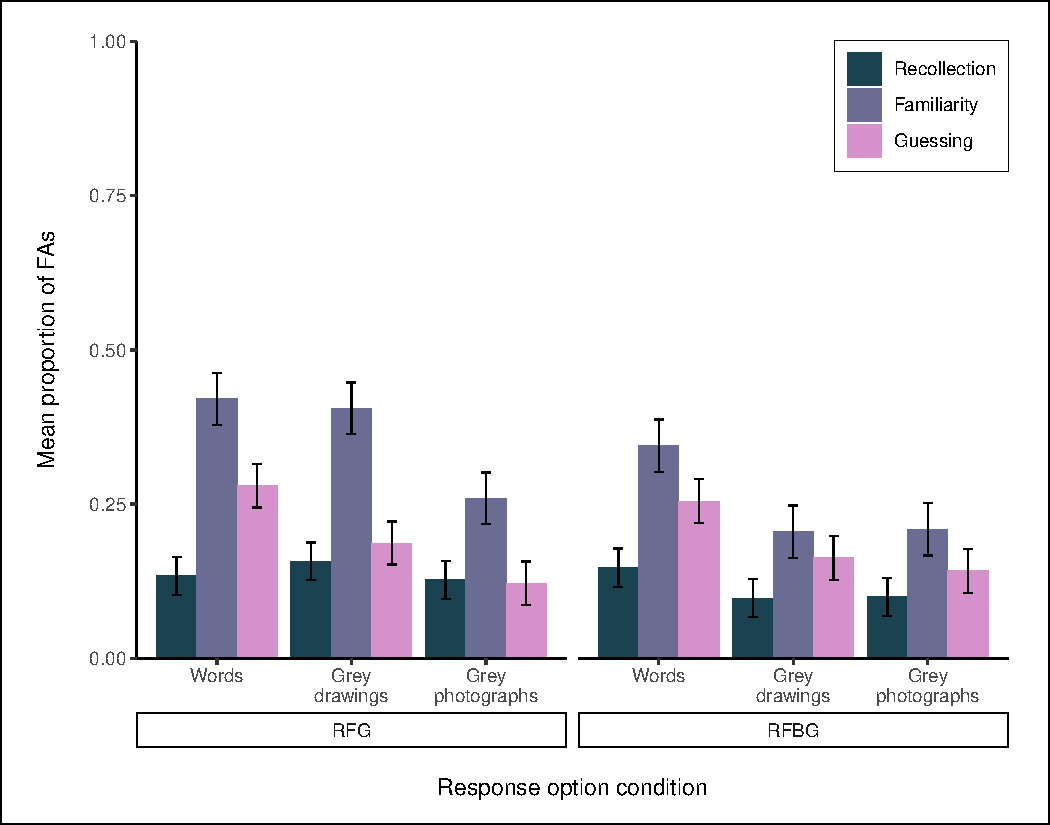
\includegraphics{R--Thesis_files/figure-latex/unnamed-chunk-50-1.pdf}
Figure 16: Proportion of FAs assigned Recollection, Familiarity, and
Guessing, by stimuli format and response option condition.

\textbf{Recollection (FAs)} For FAs assigned \emph{Recollection}, there
was no significant main effect of stimuli format {[}\emph{F}(1.92,
304.64) = 0.56, \emph{p} = .567, \(\eta^2_p\) \textless{} .01 or
interaction {[}\emph{F}(1.92, 304.64) = 1.04, \emph{p} = .352,
\(\eta^2_p\) \textless{} .01{]}.

Familiarity (FAs)

The ANOVA for FAs assigned \emph{Familiarity} showed a significant main
effect of stimuli format, \emph{F}(2, 318) = 8.66, \emph{p} \textless{}
.001, \(\eta^2_p\) = .05. Grey photographs (\emph{M}= 0.23) produced
significantly fewer F FAs than words (\emph{M}= 0.38), \emph{t}(160) =
-4.26, \emph{p} \textless{} .001; \emph{d} = -0.34, 95\% CI {[}-0.5,
-0.18{]}. Likewise, grey drawings (\emph{M}= 0.31) also showed a
significantly lower proportion of FAs compared to words (\emph{M}=
0.38), \emph{t}(160) = -1.97, \emph{p} = 0.15; \emph{d} = -0.16, 95\% CI
{[}-0.31, -0.0073{]}. However, there was no significant difference in
the proportion of FAs assigned Familiarity between grey photographs
(\emph{M}= 0.23) and grey drawings (\emph{M}= 0.31), \emph{t}(160) =
2.15, \emph{p} = 0.1; \emph{d} = 0.17, 95\% CI {[}0.02, 0.32{]}. There
were no significant interaction effects between stimuli format and
response option condition, \emph{F}(2, 318) = 2.53, \emph{p} = .081,
\(\eta^2_p\) = .02.

Guessing (FAs)

The ANOVA on the mean proportion of FAs assigned \emph{Guessing}
demonstrated a significant main effect of stimuli format \emph{F}(1.92,
305.67) = 8.95, \emph{p} \textless{} .001, \(\eta^2_p\) = .05. Grey
photographs (\emph{M}= 0.13) produced significantly fewer G FAs in
comparison to words (\emph{M}= 0.27; \emph{t}(160) = -3.98, \emph{p}
\textless{} .001; \emph{d} = -0.31, 95\% CI {[}-0.48, -0.15{]}).
Likewise, grey drawings (\emph{M}= 0.17) also showed a significantly
lower proportion of FAs compared to words (\emph{M}= 0.27; \emph{t}(160)
= -2.7, \emph{p} = 0.02; \emph{d} = -0.21, 95\% CI {[}-0.39, -0.07{]}.
However, there was no significant difference in the proportion of FAs
assigned Guessing between grey photographs (\emph{M}= 0.13) and grey
drawings (\emph{M}= 0.17; \emph{t}(160) = 1.5, \emph{p} = 0.41; \emph{d}
= 0.12, 95\% CI {[}-0.03, 0.27{]}). There were also no significant
interaction effects between stimuli format and response option condition
\emph{F}(1.92, 305.67) = 0.31, \emph{p} = .725, \(\eta^2_p\) \textless{}
.01.

\hypertarget{response-option-availability}{%
\paragraph{Response option
availability}\label{response-option-availability}}

In the previously discussed ANOVAs, significant main effects were also
observed for response option condition (RFG / RFBG) for the mean
proportion of hits (\emph{F}(1, 159) = 4.04, \emph{p} = .046,
\(\eta^2_p\) = .02) and the mean proportion of FAs assigned
\emph{Familiarity} (\emph{F}(1, 159) = 6.30, \emph{p} = .013,
\(\eta^2_p\) = .04). For all other variables, response option was found
to either significantly interact with stimuli format (discussed
previously), or had no significant main effect (see Table 7 for all
response option ANOVA results).

For the mean proportion of hits, follow up t-tests showed a higher
proportion of hits in the RFG group (\emph{M}= 0.74) compared to the
RFBG group (\emph{M}= 0.69), \emph{t}(481) = -2.37, \emph{p} = .018,
\emph{d} = 0.22. For the mean proportion of FAs assigned
\emph{Familiarity}, those in the RFG group (\emph{M}= 0.36) showed a
significantly higher proportion than those in the RFBG group (\emph{M}=
0.25), \emph{t}(480.99) = -3.12, \emph{p} = .002, \emph{d} = 0.28.

~ Table 7: Main effects of response option condition across all
variables of interest. Signif. codes: ***\emph{p} \textless{} .001;
**\emph{p} \textless{} .01; *\emph{p} \textless{} .05; + involved in
significant interaction {[}see previous section for interpretation{]}).

\begin{longtable}[]{@{}rrr@{}}
\toprule
\begin{minipage}[b]{0.38\columnwidth}\raggedleft
Variable\strut
\end{minipage} & \begin{minipage}[b]{0.46\columnwidth}\raggedleft
Main effect of response option\strut
\end{minipage} & \begin{minipage}[b]{0.07\columnwidth}\raggedleft
Signif.\strut
\end{minipage}\tabularnewline
\midrule
\endhead
\begin{minipage}[t]{0.38\columnwidth}\raggedleft
Mean proportion: \textbf{\emph{Hits}}\strut
\end{minipage} & \begin{minipage}[t]{0.46\columnwidth}\raggedleft
\emph{F}(1, 159) = 4.04, \emph{p} = .046, \(\eta^2_p\) = .02\strut
\end{minipage} & \begin{minipage}[t]{0.07\columnwidth}\raggedleft
*\strut
\end{minipage}\tabularnewline
\begin{minipage}[t]{0.38\columnwidth}\raggedleft
Mean proportion: \textbf{\emph{FAs}}\strut
\end{minipage} & \begin{minipage}[t]{0.46\columnwidth}\raggedleft
\emph{F}(1, 159) = 1.03, \emph{p} = .312, \(\eta^2_p\) \textless{}
.01\strut
\end{minipage} & \begin{minipage}[t]{0.07\columnwidth}\raggedleft
\strut
\end{minipage}\tabularnewline
\begin{minipage}[t]{0.38\columnwidth}\raggedleft
Mean scores: \textbf{\emph{d'}}\strut
\end{minipage} & \begin{minipage}[t]{0.46\columnwidth}\raggedleft
\emph{F}(1, 159) = 0.76, \emph{p} = .385, \(\eta^2_p\) \textless{}
.01\strut
\end{minipage} & \begin{minipage}[t]{0.07\columnwidth}\raggedleft
+\strut
\end{minipage}\tabularnewline
\begin{minipage}[t]{0.38\columnwidth}\raggedleft
Mean proportion: \textbf{\emph{Recollection hits}}\strut
\end{minipage} & \begin{minipage}[t]{0.46\columnwidth}\raggedleft
\emph{F}(1, 159) = 15.02, \emph{p} \textless{} .001, \(\eta^2_p\) =
.09\strut
\end{minipage} & \begin{minipage}[t]{0.07\columnwidth}\raggedleft
+\strut
\end{minipage}\tabularnewline
\begin{minipage}[t]{0.38\columnwidth}\raggedleft
Mean proportion: \textbf{\emph{Familiarity hits}}\strut
\end{minipage} & \begin{minipage}[t]{0.46\columnwidth}\raggedleft
\emph{F}(1, 159) = 2.01, \emph{p} = .159, \(\eta^2_p\) = .01\strut
\end{minipage} & \begin{minipage}[t]{0.07\columnwidth}\raggedleft
+\strut
\end{minipage}\tabularnewline
\begin{minipage}[t]{0.38\columnwidth}\raggedleft
Mean proportion: \textbf{\emph{Guessing hits}}\strut
\end{minipage} & \begin{minipage}[t]{0.46\columnwidth}\raggedleft
\emph{F}(1, 159) = 1.93, \emph{p} = .166, \(\eta^2_p\) = .01\strut
\end{minipage} & \begin{minipage}[t]{0.07\columnwidth}\raggedleft
\strut
\end{minipage}\tabularnewline
\begin{minipage}[t]{0.38\columnwidth}\raggedleft
Mean proportion: \textbf{\emph{Recollection FAs}}\strut
\end{minipage} & \begin{minipage}[t]{0.46\columnwidth}\raggedleft
\emph{F}(1, 159) = 0.58, \emph{p} = .446, \(\eta^2_p\) \textless{}
.01\strut
\end{minipage} & \begin{minipage}[t]{0.07\columnwidth}\raggedleft
\strut
\end{minipage}\tabularnewline
\begin{minipage}[t]{0.38\columnwidth}\raggedleft
Mean proportion: \textbf{\emph{Familiarity FAs}}\strut
\end{minipage} & \begin{minipage}[t]{0.46\columnwidth}\raggedleft
\emph{F}(1, 159) = 6.30, \emph{p} = .013, \(\eta^2_p\) = .04\strut
\end{minipage} & \begin{minipage}[t]{0.07\columnwidth}\raggedleft
*\strut
\end{minipage}\tabularnewline
\begin{minipage}[t]{0.38\columnwidth}\raggedleft
Mean proportion: \textbf{\emph{Guessing FAs}}\strut
\end{minipage} & \begin{minipage}[t]{0.46\columnwidth}\raggedleft
\emph{F}(1, 159) = 0.08, \emph{p} = .772, \(\eta^2_p\) \textless{}
.01\strut
\end{minipage} & \begin{minipage}[t]{0.07\columnwidth}\raggedleft
\strut
\end{minipage}\tabularnewline
\bottomrule
\end{longtable}

\hypertarget{discussion-2}{%
\subsubsection{Discussion}\label{discussion-2}}

Across a range of performance variables, the results show a clear effect
of stimuli distinctiveness. As distinctiveness increased (from words, to
drawings, to photographs), this produced more hits, less FAs, better
overall recognition, and better discrimination between hits / FAs. The
absence of any interaction effects across these variables demonstrates
that the availability of different response options (i.e.~the addition
of a Both option) had little impact on overall performance. RF(B)G
responses for accurate recognition displayed a similar pattern; as
distinctiveness increased, the number of Recollected hits also
increased, while the number of Familiarity and Guessing hits decreased.
The rate of both Familiarity FAs and Guessing FAs was also highest for
the least distinctive stimuli (words).

\#\#\#\#\#\#----------------------------------------

\newpage

\hypertarget{chapter-4---the-role-of-colour}{%
\section{Chapter 4 - The role of
colour}\label{chapter-4---the-role-of-colour}}

\hypertarget{background-2}{%
\subsection{Background}\label{background-2}}

In Chapter 3, the role of stimuli distinctiveness on recognition was
explored by curating a new set of detailed, real-world object
photographs, and comparing recognition performance toward these items
with matched shaded drawn images and written word counterparts. Standard
picture superiority effects (PSEs) were observed, with both types of
picture producing enhanced recognition performance compared to word
stimuli, however, a clear \emph{photograph} superiority effect was also
evident when comparisons were made between the photographs and drawings.
Such results were attributed to the physical distinctiveness account of
the PSE, whereby increased item-to-item variability results in items
being remembered better than those with low variability. Studies have
previously offered support for this hypothesis by attempting to
manipulate the level of variability between items; Ensor et al. (2019)
demonstrated how the PSE could be eliminated by i) increasing the
variability between word stimuli, where each item was made more
distinctive by manipulations to font, size, and colour, and ii) reducing
the variability between picture stimuli, where shaded drawing items
consisted of objects with highly similar shapes, size, and orientation.
The current programme of research extended support for this hypothesis
by increasing the variability between picture stimuli through the
creation of a set of photographic stimuli where differences in detail,
texture, and shading were intended to be more apparent across items than
across drawings. While the \emph{photograph} superiority effect (PhSE)
demonstrated in the previous study highlights the importance of real
world texture and shading in recognition memory, there are other
inconsistencies across recognition memory studies with regard to
distinctiveness - namely, whether images are presented to participants
in greyscale or colour.

The extent to which colour affects the memorability of stimuli is
unclear, though there is evidence to suggest this additional layer of
information may increase the perceived distinctiveness of items. In a
scene recognition paradigm, Suzuki \& Takahashi (1997) demonstrated that
black \& white images may not facilitate successful recognition in the
same way as colour images. In an initial study phase, subjects were
instructed to passively memorise a number of real-world scene
photographs (e.g.~train stations, city streets etc.). At test,
participants were presented with two photographs side-by-side (one
target + one similar lure) and asked to select the item shown during the
study phase. The congruency of colour was manipulated, such that
photographs were either presented in the same colour modality across
both study and test (1. greyscale at study / greyscale at test; 2.
colour at study / colour at test) or different (3. greyscale at study /
colour at test; 4. colour at study / greyscale at test). Results showed
that colour information produced superior recognition performance when
presented congruently across encoding and retrieval. Interestingly, this
colour benefit was \emph{only} evident in the congruent condition; if
colour images were paired with greyscale images - regardless of the
order at encoding and test - recognition benefits were absent. A source
judgement question at test, probing whether the colour format for each
item was the same or different as at study showed similar performance
across all four conditions (though performance was particularly poor for
items presented in colour); such findings indicate the recognition
benefits of the congruent colour condition were not a result of
accessing memory for the colour information itself, but rather colour
indirectly highlighted certain features within the photographs that were
not otherwise noticed as prominently in greyscale, and thus the colour
photographs were overall more distinctive as a result.

The current experiment aims to establish whether colour information
facilitates successful recognition using object stimuli. The methodology
of \emph{Experiment 3} is precisely replicated - whereby recognition is
tested across word, drawing, and photograph stimuli - though rather than
greyscale items, the sole manipulation of the current study is the
addition of colour to the two types of image stimuli. Initial analyses
will determine whether the distinctiveness effects of the previous study
are also evident when colour items are utilised, and in particular,
whether a \emph{photo} superiority effect remains, or if this finding is
unique to greyscale stimuli. It is acknowledged that colour may not
affect the two types of image in a uniform manner. The highly
distinctiveness nature of the photograph items may plateau in such a way
that performance can no longer be noticeably enhanced; any additional
distinctiveness generated by colour information might show little
benefit if performance is already sufficiently high. If this is the
case, however, the effects of the colour manipulation should still be
evident when examining recognition performance for drawings, where there
is more room for such benefits to become apparent. Following this
initial analysis, exploratory comparisons will be made to compare the
data from the current experiment with that from \emph{Experiment 3}, in
an effort to highlight any key differences introduced by the addition of
colour. A secondary aim from previous experiments remains, whereby the
role of different available response options
(\emph{Recollection}/\emph{Familiarity}/\emph{Guessing} or
\emph{Recollection}/\emph{Familiarity}/\emph{Both}/\emph{Guessing}) will
be examined to establish whether RFG response patterns are
differentially affected following the introduction of colour. The
following hypotheses are proposed:

\begin{enumerate}
\def\labelenumi{\arabic{enumi}.}
\item
  A photograph superiority effect (similar to that observed in
  \emph{Experiment 3}) will again be evident, whereby photograph items
  produce better recognition performance compared to drawings. Based on
  the results of the previous study, this performance benefit is
  expected to manifest as:

  \begin{itemize}
  \item
    \begin{enumerate}
    \def\labelenumii{\roman{enumii})}
    \tightlist
    \item
      a higher proportion of correct hits;
    \end{enumerate}
  \item
    \begin{enumerate}
    \def\labelenumii{\roman{enumii})}
    \setcounter{enumii}{1}
    \tightlist
    \item
      a lower proportion of false alarms (FAs);
    \end{enumerate}
  \item
    \begin{enumerate}
    \def\labelenumii{\roman{enumii})}
    \setcounter{enumii}{2}
    \tightlist
    \item
      higher overall \emph{d'} scores.
    \end{enumerate}
  \end{itemize}
\item
  Colour information will enhance the relative distinctiveness of image
  stimuli, resulting in enhanced recognition performance compared to
  previously utilised greyscale items. Exploratory analyses comparing
  the results of the current study with those of \emph{Experiment 3} are
  expected to reveal numerical differences between the colour and
  greyscale findings, such that the colour items exhibit performance
  enhancements in the same direction as those outlined in Hypothesis 1
  when compared to the greyscale items.
\item
  Any effects associated with manipulating the availability of response
  options at test (RFG/RFBG) will remain unaffected by the addition of
  colour information to image stimuli. Based on the findings of
  \emph{Experiment 3}, it is expected that:

  \begin{itemize}
  \item
    \begin{enumerate}
    \def\labelenumii{\roman{enumii})}
    \tightlist
    \item
      The RFG group will produce a significantly higher proportion of
      overall hits compared to the RFBG group.
    \end{enumerate}
  \item
    \begin{enumerate}
    \def\labelenumii{\roman{enumii})}
    \setcounter{enumii}{1}
    \tightlist
    \item
      The RFG group will produce a significantly higher proportion of
      FAs assigned \emph{Familiarity} compared to the RFBG group.
    \end{enumerate}
  \item
    \begin{enumerate}
    \def\labelenumii{\roman{enumii})}
    \setcounter{enumii}{2}
    \tightlist
    \item
      Significant interaction effects between response option and
      stimuli format will be evident in the analyses of mean \emph{d'}
      scores, mean proportion of hits assigned \emph{Recollection}, and
      mean proportion of hits assigned \emph{Familiarity}.
    \end{enumerate}
  \end{itemize}
\end{enumerate}

~~

\hypertarget{experiment-effect-of-stimuli-format-colour-and-response-option-on-recognition-memory-judgements.}{%
\subsection{Experiment: Effect of stimuli format (colour) and response
option on recognition memory
judgements.}\label{experiment-effect-of-stimuli-format-colour-and-response-option-on-recognition-memory-judgements.}}

\hypertarget{method-3}{%
\subsubsection{Method}\label{method-3}}

\hypertarget{participants-3}{%
\paragraph{Participants}\label{participants-3}}

\hfill\break 164 participants completed the experiment online (see Table
8 for a breakdown of the age/gender of the current sample). All
participants were required to be between the age of 18-59 years in order
to meet our YA criteria (actual range: 18-57). As our experiment
involved written words as to-be-remembered stimuli, we also asked that
subjects first language be English; the vast majority (96.95\%) reported
that English was indeed their first language. Subjects were recruited
from the voluntary participation website
Prolific Academic\footnote{\url{https://www.prolific.co/}} (85.98\%),
where payment at the rate of £5/hr was given, and via the in-school
research participation system\footnote{\url{https://keelepsychology.sona-systems.com/}}
(14.02\%), where they received course participation credits.
\emph{G*Power} software was used to calculate an appropriate sample
size; to detect a medium effect size of Cohen's \emph{f} = 0.25 with
80\% power (\emph{α} = .05, two-tailed), 79 subjects per group would be
necessary (\emph{N} = 158) in a 3x2 mixed ANOVA.

\newpage

Table 8: Gender and age (\emph{SD}) of the current sample.

\begin{table}[!h]
\centering
\begin{tabular}{l>{}rr>{}l}
\toprule
Gender & N & Age &  \\
\midrule
Female & \em{99} & 31.72 & \em{(11.16)}\\
Male & \em{61} & 31.87 & \em{(10.25)}\\
Non-binary & \em{1} & 19.00 & \em{(0)}\\
Transgender & \em{1} & 32.00 & \em{(0)}\\
\textbf{Unspecified} & \textbf{\em{2}} & \textbf{38.50} & \textbf{\em{(3.54)}}\\
\addlinespace
Total & \em{164} & 31.78 & \em{(10.73)}\\
\bottomrule
\end{tabular}
\end{table}

\hypertarget{materials-3}{%
\paragraph{Materials}\label{materials-3}}

\hfill\break Stimuli were the same as those utilised in \emph{Experiment
3}, except the greyscale drawings and photographs were substituted for
their colour versions. Items consisted of 126 innocuous, everyday
objects (e.g.~clock, rabbit, shoe), presented across three individual
stimuli formats: written words, shaded drawings, and photographs. Words
and shaded drawings were sourced from Rossion \& Pourtois (2004); the
drawings consisted of shaded, colour illustrations, and the words were
simply the written names of the depicted objects (these were presented
in a clear Sans-serif typeface in the current experiment). A matching
set of photograph stimuli were curated in \emph{Experiment 2}; high
quality photographs were sourced to similarly depict the same everyday
objects as those found in the Rossion \& Pourtois (2004) shaded
drawings. In each photograph, the object of interest was isolated from
its original background and rotated to match the orientations shown in
the line-drawn items. See Figure 17 for examples of each stimuli format.

\hypertarget{design-3}{%
\paragraph{Design}\label{design-3}}

\hfill\break A mixed 3x2 design was utilised, consisting of a
within-subjects factor of stimuli format (words, drawings, photographs)
and a between-subjects factor of response option (RFG, RFBG).
Counterbalancing was achieved via blocked randomisation, whereby
participants were presented with: 1) one of six possible study lists
(equal length, with the same number of words, drawings, and
photographs); 2) one of two possible recognition tests (either RFG:
``Recollection'', ``Familiarity'', ``Guessing''), or RFBG:
``Recollection'', ``Familiarity'', ``Guessing'', ``Both''). All
counterbalancing routes were of equal length, and subjects were randomly
assigned into blocks via balanced methods.

\hypertarget{procedure-3}{%
\paragraph{Procedure}\label{procedure-3}}

\hfill\break The procedure was identical to that of \emph{Experiment 3};
data collection was conducted online using the experiment platform
Gorilla\footnote{\url{https://gorilla.sc/}}. All subjects completed
three self-paced phases: i) study phase, ii) distractor task, and iii)
recognition test. At study, subjects were instructed to learn each of
the word, drawing, and photograph items (shown at random, one-at-a-time)
in preparation for a later memory test. For each item, participants were
required to report whether the current format was a word, drawing, or
photograph - an encoding judgement that ensured attention was directed
toward the to-be-remembered stimuli. Next, subjects completed some
simple multiple choice mathematical questions (e.g.~6 x 4 = ?) as a
distractor task. Finally, participants were presented with the
recognition test; word, drawing, and photograph items were once again
shown one-at-a-time at random. Half of the test items had been shown
previously in the study phase, while the other half were new (not shown
at study). Subjects were first required to make an \emph{Old}/\emph{New}
judgement, based on whether they believed they had studied the item
earlier or not. While \emph{New} judgements simply led to the next item,
\emph{Old} judgements led to a follow-up screen where participants were
asked whether they had recognised the item via \emph{Recollection},
\emph{Familiarity}, or were simply \emph{Guessing} that it was old.
Those in the RFBG response option condition had an additional
\emph{Both} option at this stage, where they could report that they had
experienced recollection and familiarity simultaneously. Stimuli format
stayed the same across study and test (e.g.~if the item ``penguin'' was
shown in word format at study, it was also shown as a word at test), and
the same concepts were not repeated across the other formats
within-subjects (e.g.~if the item ``penguin'' was shown as a word, that
subject would not view the drawing or photo version).

~ ~

\includegraphics[width=1\linewidth]{./resources/images/exp4__stim_examples}
Figure 17: Examples of the word, colour drawing, and colour photograph
stimuli utilised in the current experiment. ~ ~

\hypertarget{data-processing-3}{%
\paragraph{Data processing}\label{data-processing-3}}

\hfill\break The primary DVs of interest consisted of the mean
proportion of hits and false alarms (FAs), mean \emph{d'} scores
(d-prime, a signal detection measure of sensitivity), and the total
number of hits and FAs assigned to each of the available response
options (R/F/G or R/F/B/G). Proportions of Recollection and Familiarity
were calculated slightly differently depending on the response option
condition; in the RFG-judgement group, simple proportions were created
from the total number of R responses and the total number of F
responses. In the RFBG condition, the proportion of Both responses were
added separately to R proportions and F proportions. All analyses were
conducted with \emph{R} (R Core Team, 2020) using the \emph{afex}
(v0.28-0; Singmann et al., 2020) and \emph{rstatix} packages (v0.6.0;
Kassambara, 2020).

Subjects were excluded from analyses on the basis of two key criteria;
1) less than 90\% accuracy during the encoding task (``Is this a word,
drawing, or photograph?''); 2) extreme z-scores (those presenting
z-scores of +/- 3 for total hits, total FAs, or overall recognition
{[}hits minus FAs{]}). A total of 3 participants were found to meet (at
least) one of these criteria, and were thus considered outliers and
excluded from analysis, leaving a total of 161 datasets.

\hypertarget{results-3}{%
\subsubsection{Results}\label{results-3}}

A series of 3x2 mixed ANOVAs were conducted on each of the DVs, with a
within-subjects factor of stimuli format (words / colour drawings /
colour photos) and a between-subjects factor of response option (RFG /
RFBG). Significant main effects and interaction effects were followed-up
with Bonferroni-adjusted pairwise comparisons. Greenhouse-Geisser
corrections were applied when ANOVA data was found to violate the
assumption of sphericity (assessed according to Mauchly's test
statistic).

\hypertarget{stimuli-distinctiveness-1}{%
\paragraph{Stimuli distinctiveness}\label{stimuli-distinctiveness-1}}

\hfill\break Mean proportions of hits and FAs, and mean \emph{d'} scores
are presented for Experiments 3 and 4 in Table 9. Visual inspection of
the data shows some expected patterns with regard to stimuli
distinctiveness. As the intended distinctiveness increases (from words,
to drawings, to photographs), the i) mean proportion of hits increase;
ii) mean proportion of FAs decrease; iii) mean \emph{d'} scores
increase.

Results from the ANOVAs demonstrated a significant main effect of
stimuli format for each of the key variables of interest; hits
(\emph{F}(1.70, 271.03) = 187.25, \emph{p} \textless{} .001,
\(\eta^2_p\) = .54), FAs (\emph{F}(1.26, 200.79) = 123.14, \emph{p}
\textless{} .001, \(\eta^2_p\) = .44), and \emph{d'} scores (\emph{F}(2,
318) = 465.93, \emph{p} \textless{} .001, \(\eta^2_p\) = .75) - though
no interaction effects were evident between stimuli format and response
option; hits (\emph{F}(1.70, 271.03) = 1.22, \emph{p} = .291,
\(\eta^2_p\) \textless{} .01), FAs(\emph{F}(1.26, 200.79) = 2.72,
\emph{p} = .092, \(\eta^2_p\) = .02), or \emph{d'} scores (\emph{F}(2,
318) = 0.20, \emph{p} = .817, \(\eta^2_p\) \textless{} .01).

\newpage

Table 9: Data from Experiment 3 (using greyscale stimuli) shown
alongside that of the current experiment (using colour stimuli), showing
the mean proportion of hits, FAs, and mean \emph{d'} scores, by stimuli
format and response option condition. Signif. codes: ***\emph{p}
\textless{} .001; **\emph{p} \textless{} .01; *\emph{p} \textless{} .05;
+ involved in significant interaction.

\begin{table}[!h]
\centering\begingroup\fontsize{13}{15}\selectfont

\resizebox{\linewidth}{!}{
\begin{tabular}{>{\raggedright\arraybackslash}p{1.9cm}>{\raggedright\arraybackslash}p{2.5cm}>{\centering\arraybackslash}p{1cm}>{\centering\arraybackslash}p{1cm}>{\centering\arraybackslash}p{1cm}>{\centering\arraybackslash}p{1.8cm}>{\raggedright\arraybackslash}p{1.9cm}>{\raggedright\arraybackslash}p{2.5cm}>{\centering\arraybackslash}p{1cm}>{\centering\arraybackslash}p{1cm}>{\centering\arraybackslash}p{1cm}}
\toprule
\multicolumn{2}{c}{\textbf{Experiment 3: Grey}} & \multicolumn{4}{c}{\textbf{ }} & \multicolumn{2}{c}{\textbf{Experiment 4: Colour}} \\
  &    & Hits & FAs & d' &      &       &     & Hits & FAs & d'\\
\midrule
\textbf{Stimuli format:} & \textbf{} & \textbf{***} & \textbf{***} & \textbf{+} & \textbf{} & \textbf{Stimuli format:} & \textbf{} & \textbf{***} & \textbf{***} & \textbf{***}\\
 & Words & 0.54 & 0.21 & 1.15 &  &  & Words & 0.55 & 0.23 & 1.11\\
 & Drawings & 0.76 & 0.09 & 2.38 &  &  & Drawings & 0.73 & 0.08 & 2.39\\
 & Photographs & 0.85 & 0.05 & 3.08 &  &  & Photographs & 0.87 & 0.04 & 3.25\\
\textbf{Response option:} & \textbf{} & \textbf{*} & \textbf{} & \textbf{+} & \textbf{} & \textbf{Response option:} & \textbf{} & \textbf{} & \textbf{*} & \textbf{}\\
\addlinespace
 & RFG & 0.74 & 0.13 & 2.25 &  &  & RFG & 0.74 & 0.13 & 2.25\\
 & RFBG & 0.69 & 0.11 & 2.16 &  &  & RFBG & 0.7 & 0.1 & 2.25\\
\bottomrule
\end{tabular}}
\endgroup{}
\end{table}

~ ~

To determine whether photo superiority effects were exhibited in the
current set of colour stimuli - comparable to those previously observed
using greyscale items (Experiment 3) - pairwise t-tests were performed
between the colour photos and drawings. For the mean proportion of hits,
colour photographs (\emph{M}= 0.87) exhibited a significantly higher
proportion than colour drawings (\emph{M}= 0.73), \emph{t}(160) =
-11.04, \emph{p} \textless{} .001; \emph{d} = -0.87, 95\% CI {[}-1.02,
-0.74{]}. The photographs (\emph{M}= 0.04) also produced significantly
fewer FAs compared to drawings (\emph{M}= 0.08), \emph{t}(160) = 6.36,
\emph{p} \textless{} .001; \emph{d} = 0.5, 95\% CI {[}0.37, 0.64{]}).
Mean \emph{d'} scores were also significantly higher for the colour
photographs (\emph{M}= 3.25) compared to the colour drawings (\emph{M}=
2.39), \emph{t}(160) = -13.56, \emph{p} \textless{} .001; \emph{d} =
-1.07, 95\% CI {[}-1.27, -0.89{]}. These findings replicate those found
previously using greyscale items, whereby photographs offer a number of
recognition benefits when compared to less detailed line-drawn
illustrations.

Visual inspection of the data (and significant results) reveals only one
difference with regard to response option when compared to that obtained
in \emph{Experiment 3}: the ANOVA on \emph{d'} scores failed to produce
a significant interaction between stimuli format and response option in
the current experiment, as was previously demonstrated. Previous
follow-up comparisons revealed this interaction was driven by
numerically higher \emph{d'} scores for drawings in the RFBG group
compared to the RFG group - a deviation from words and photographs,
whereby \emph{d'} scores were both higher in the RFG group compared to
the RFBG group. The difference between \emph{d'} scores for drawings in
the RFG and RFBG groups did not reach significance though, and this
negligible difference may explain why such an interaction was absent in
the current study.

\hypertarget{recollection-and-familiarity-1}{%
\paragraph{Recollection and
Familiarity}\label{recollection-and-familiarity-1}}

\hfill\break To determine the effects of stimuli format and response
option on the classification of recognition memory judgements, separate
3 (stimuli format: words, drawings, photographs) x 2 (response option
condition: RFG-judgements, RFBG-judgements) mixed ANOVAs were conducted
on the mean proportion of hits assigned Recollection, Familiarity, and
Guessing (see Figure 18).

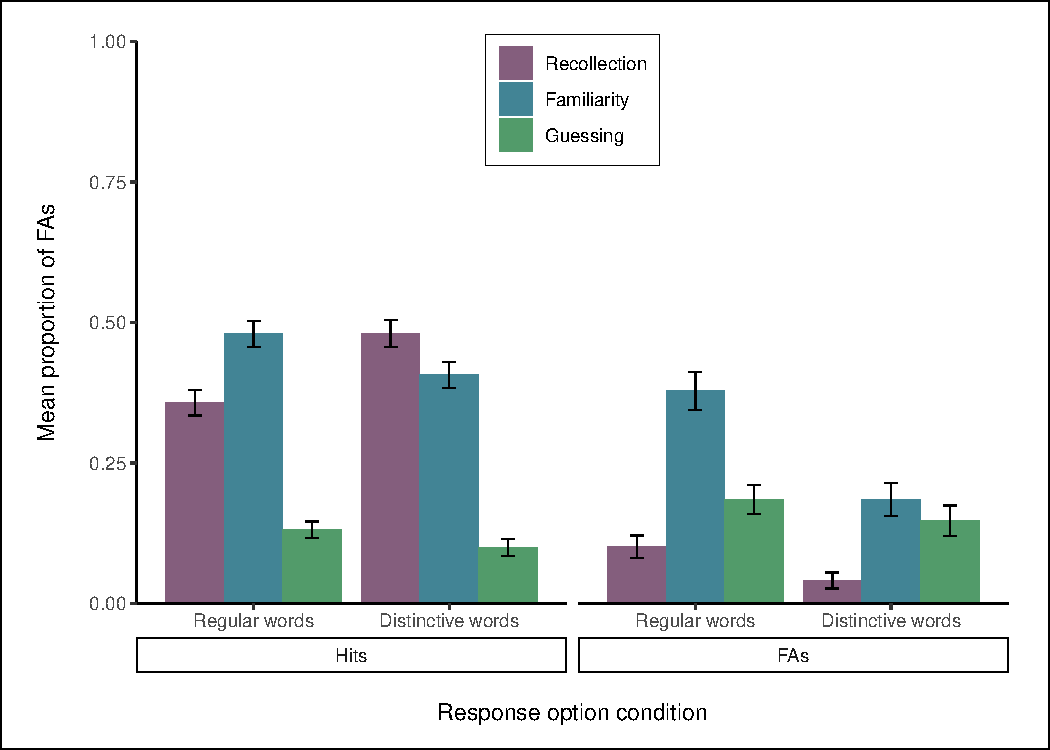
\includegraphics{R--Thesis_files/figure-latex/unnamed-chunk-63-1.pdf}
Figure 18: Proportion of hits assigned Recollection, Familiarity, and
Guessing, by stimuli format and response option condition.

\textbf{Recollection (hits):} Results from the ANOVA on the mean
proportion of hits assigned Recollection showed a significant
interaction between stimuli format and response option condition,
\emph{F}(1.39, 221.56) = 10.79, \emph{p} \textless{} .001, \(\eta^2_p\)
= .06 (see Figure 19).

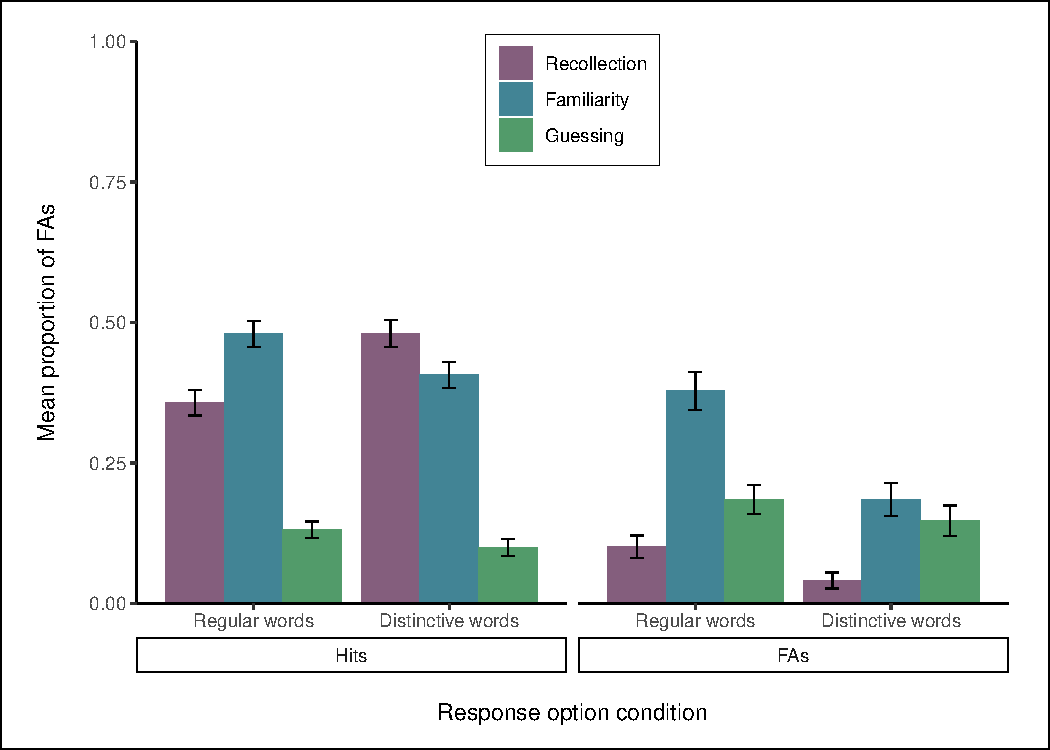
\includegraphics{R--Thesis_files/figure-latex/unnamed-chunk-65-1.pdf}
Figure 19: Interaction plot between stimuli format and response option
for the mean proportion of hits assigned Recollection.

Comparisons across stimuli formats showed colour photographs produced a
significantly higher proportion of R hits than both words and colour
drawings in both the RFG group (colour photographs {[}\emph{M}= 0.76{]}
vs.~words {[}\emph{M}= 0.32{]}, \emph{t}(318) = -15.02, \emph{p}
\textless{} .001; colour photographs {[}\emph{M}= 0.76{]} vs.~colour
drawings {[}\emph{M}= 0.63{]}, \emph{t}(318) = -4.53, \emph{p}
\textless{} .001) and the RFBG group (colour photographs {[}\emph{M}=
0.56{]} vs.~words {[}\emph{M}= 0.3{]}, \emph{t}(318) = -8.17, \emph{p}
\textless{} .001; colour photographs {[}\emph{M}= 0.56{]} vs.~colour
drawings {[}\emph{M}= 0.46{]}, \emph{t}(318) = -3.11, \emph{p} = .031).
Likewise, colour drawings produced a significantly higher proportion of
R hits in comparison to Words in both the RFG (colour drawings
{[}\emph{M}= 0.63{]} vs.~words {[}\emph{M}= 0.32{]}, \emph{t}(318) =
-10.49, \emph{p} \textless{} .001) and RFBG conditions (colour drawings
{[}\emph{M}= 0.46{]} vs.~words {[}\emph{M}= 0.3{]}, \emph{t}(318) =
-5.06, \emph{p} \textless{} .001).

The interaction is evident following comparisons of the same stimuli
format across response option conditions. The RFG group produced a
significantly higher proportion of R hits than the RFBG group for colour
photographs (RFG {[}\emph{M} = 0.76{]} vs.~RFBG {[}\emph{M} = 0.56{]},
\emph{t}(274.37) = -4.19, \emph{p} = .001) and for colour drawings (RFG
{[}\emph{M} = 0.63{]} vs.~RFBG {[}\emph{M} = 0.46{]}, \emph{t}(274.37) =
-3.43, \emph{p} = .011). However, this was not the case for words, where
there was no difference in the proportion of R hits between the RFG
(\emph{M} = 0.32) and RFBG groups (\emph{M} = 0.3; \emph{t}(274.37) =
-0.30, \emph{p} \textgreater{} .999).

\textbf{Familiarity (hits):} Results from the ANOVA on the mean
proportion of hits assigned Familiarity again showed a significant main
effect of stimuli format \emph{F}(1.49, 236.15) = 50.18, \emph{p}
\textless{} .001, \(\eta^2_p\) = .24. Colour photographs (\emph{M}= 0.2)
produced significantly fewer F hits than both words (\emph{M}= 0.42),
\emph{t}(160) = -8.34, \emph{p} \textless{} .001; \emph{d} = -0.66, 95\%
CI {[}-0.84, -0.49{]}, and colour drawings (\emph{M}= 0.29),
\emph{t}(160) = 5.97, \emph{p} \textless{} .001; \emph{d} = 0.47, 95\%
CI {[}0.31, 0.65{]}. The colour drawings (\emph{M}= 0.29) also showed
significantly fewer F hits compared to words (\emph{M}= 0.42),
\emph{t}(160) = -5.77, \emph{p} \textless{} .001; \emph{d} = -0.45, 95\%
CI {[}-0.64, -0.3{]}. There were no significant interaction effects
between stimuli format and response option condition, \emph{F}(1.49,
236.15) = 1.33, \emph{p} = .263, \(\eta^2_p\) \textless{} .01.

\textbf{Guessing (hits):} The ANOVA on the mean proportion of hits
assigned Guessing demonstrated a significant main effect of stimuli
format \emph{F}(1.29, 204.70) = 82.24, \emph{p} \textless{} .001,
\(\eta^2_p\) = .34. Colour photographs (\emph{M}= 0.02) produced
significantly fewer G hits in comparison to both words (\emph{M}= 0.22;
\emph{t}(160) = -10.18, \emph{p} \textless{} .001; \emph{d} = -0.8, 95\%
CI {[}-0.92, -0.7{]}) and colour drawings (\emph{M}= 0.07; \emph{t}(160)
= 5.5, \emph{p} \textless{} .001; \emph{d} = 0.43, 95\% CI {[}0.32,
0.55{]}). The colour drawings (\emph{M}= 0.07) also showed a
significantly lower proportion of G hits compared to words (\emph{M}=
0.22; \emph{t}(160) = -8.41, \emph{p} \textless{} .001; \emph{d} =
-0.66, 95\% CI {[}-0.79, -0.54{]}. There were no significant interaction
effects between stimuli format and response option condition
\emph{F}(1.29, 204.70) = 0.09, \emph{p} = .824, \(\eta^2_p\) \textless{}
.01.

Separate 3 (stimuli format: words, drawings, photographs) x 2 (response
option condition: RFG-judgements, RFBG-judgements) mixed ANOVAs were
also conducted on the mean proportion of FAs assigned Recollection,
Familiarity, and Guessing (see Figure 20).

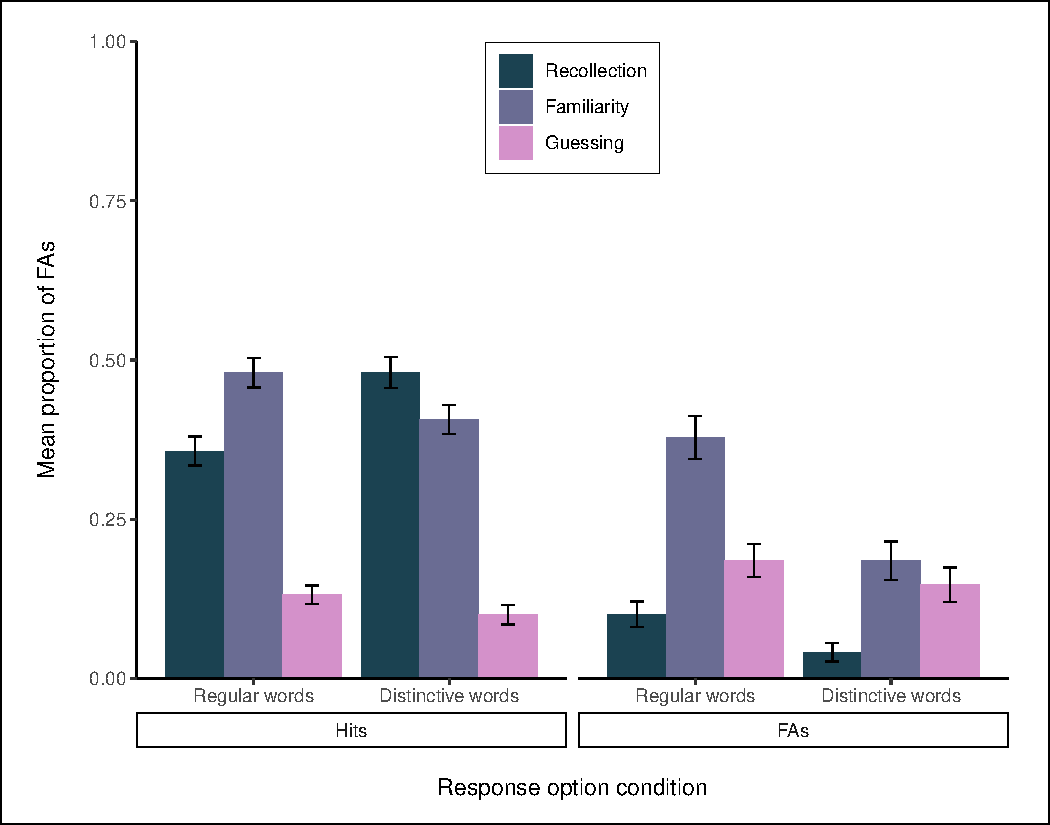
\includegraphics{R--Thesis_files/figure-latex/unnamed-chunk-68-1.pdf}
Figure 20: Proportion of FAs assigned Recollection, Familiarity, and
Guessing, by stimuli format and response option condition.

\textbf{Recollection (FAs):} For FAs assigned \emph{Recollection}, there
was no significant main effect of stimuli format {[}\emph{F}(2, 318) =
1.58, \emph{p} = .207, \(\eta^2_p\) \textless{} .01 or interaction
{[}\emph{F}(2, 318) = 0.32, \emph{p} = .727, \(\eta^2_p\) \textless{}
.01{]}.

\textbf{Familiarity (FAs):} The ANOVA for FAs assigned
\emph{Familiarity} showed a significant main effect of stimuli format,
\emph{F}(2, 318) = 22.92, \emph{p} \textless{} .001, \(\eta^2_p\) = .13.
Colour photographs (\emph{M}= 0.16) produced significantly fewer F FAs
than words (\emph{M}= 0.4), \emph{t}(160) = -6.41, \emph{p} \textless{}
.001; \emph{d} = -0.51, 95\% CI {[}-0.69, -0.36{]}. Likewise, colour
drawings (\emph{M}= 0.31) also showed a significantly lower proportion
of FAs compared to words (\emph{M}= 0.4), \emph{t}(160) = -2.45,
\emph{p} = 0.05; \emph{d} = -0.19, 95\% CI {[}-0.35, -0.05{]}. However,
there was no significant difference in the proportion of FAs assigned
Familiarity between colour photographs (\emph{M}= 0.16) and colour
drawings (\emph{M}= 0.31), \emph{t}(160) = 4.65, \emph{p} \textless{}
.001; \emph{d} = 0.37, 95\% CI {[}0.22, 0.53{]}. There were no
significant interaction effects between stimuli format and response
option condition, \emph{F}(2, 318) = 0.70, \emph{p} = .498, \(\eta^2_p\)
\textless{} .01.

\textbf{Guessing (FAs):} The ANOVA on the mean proportion of FAs
assigned \emph{Guessing} demonstrated a significant main effect of
stimuli format \emph{F}(2, 318) = 16.11, \emph{p} \textless{} .001,
\(\eta^2_p\) = .09. Colour photographs (\emph{M}= 0.15) produced
significantly fewer G FAs in comparison to words (\emph{M}= 0.31),
\emph{t}(160) = -4.5, \emph{p} \textless{} .001; \emph{d} = -0.35, 95\%
CI {[}-0.53, -0.21{]}). Likewise, colour drawings (\emph{M}= 0.15) also
showed a significantly lower proportion of FAs compared to words
(\emph{M}= 0.31), \emph{t}(160) = -4.85, \emph{p} \textless{} .001;
\emph{d} = -0.38, 95\% CI {[}-0.54, -0.23{]}. However, there was no
significant difference in the proportion of FAs assigned Guessing
between colour photographs (\emph{M}= 0.15) and colour drawings
(\emph{M}= 0.15), \emph{t}(160) = -0.15, \emph{p} = 1; \emph{d} = -0.01,
95\% CI {[}-0.16, 0.14{]}). There were also no significant interaction
effects between stimuli format and response option condition \emph{F}(2,
318) = 1.57, \emph{p} = .210, \(\eta^2_p\) \textless{} .01.

Visual inspection of the data in Figure 18 and Figure 20 demonstrates a
highly similar pattern of responding between \emph{Experiment 3} and the
current study, and suggest the addition of colour had little impact on
RFG response patterns.

\hypertarget{response-option-availability-1}{%
\paragraph{Response option
availability}\label{response-option-availability-1}}

\hfill\break In each of the aforementioned ANOVAs, the role of response
option was also examined to determine whether the addition of colour
information had any differential effects compared to the findings of
\emph{Experiment 3}. The only main effect of response option was
observed in the ANOVA for the mean proportion of FAs (\emph{F}(1, 159) =
1.03, \emph{p} = .312, \(\eta^2_p\) \textless{} .01), whereby a higher
proportion of FAs was evident in the RFG group (\emph{M}= 0.13) compared
to the RFBG group (\emph{M}= 0.1), \emph{t}(457.34) = -2.43, \emph{p} =
.016, \emph{d} = 0.22. Such results do not support Hypothesis 3, where
significant main effects of response option were expected in the ANOVAs
for the mean proportion of hits and mean proportion of FAs assigned
\emph{Familiarity}. Similarly, the expected interactions for mean
\emph{d'} scores and proportion of hits assigned \emph{Familiarity} were
also absent. The only consistent finding across \emph{Experiment 3} and
the current experiment (with regard to response option) comes from the
ANOVA for the mean proportion of hits assigned \emph{Recollection} -
where a significant interaction between stimuli format and response
option was apparent in both experiments; in both experiments, the
proportion of R hits did not differ across RFG and RFBG groups for word
stimuli, whereas for drawings and photographs, the RFG group produced a
significantly higher proportion of R hits than the RFBG group.

\hypertarget{discussion-3}{%
\subsubsection{Discussion}\label{discussion-3}}

The aim of the current experiment was to determine the effects of colour
on recognition performance. In \emph{Experiment 3}, recognition
performance was found to improve in a linear manner as the intended
distinctiveness of greyscale items increased, from words to shaded
drawings to photographs. While standard PSEs were expected, the most
notable finding of the previous study was the superiority of photographs
compared to drawings - a result that offered support for the physical
distinctiveness account of the PSE over dual-coding theory. In the
current experiment, the physical distinctiveness of image stimuli was
manipulated through the addition of colour; it was hypothesised that
colour would provide an additional layer of distinctive information that
would further facilitate successful recognition. When comparing the
results of the current study with those obtained in \emph{Experiment 3},
this hypothesis appears wholly unsupported; colour had little to no
impact on the proportion of hits, FAs, and overall recognition accuracy.

The current results continue to be best explained by the physical
distinctiveness account of the PSE. Across each of the key variables,
photographs demonstrated clear recognition benefits compared to
drawings, replicating that found in \emph{Experiment 3} and further
supporting the notion that the current set of stimuli appear to
effectively capture different `levels' of stimuli distinctiveness. The
additional real-world detail present in the photographs, and the
increased variability between items as a result, provides memorial
advantages over simple illustrated representations of objects. The key
manipulation in the current study - the addition of colour - was
unsuccessful in providing an additional layer of distinctiveness that
would further enhance recognition for the objects compared to when they
are presented in greyscale. Failure to discern any impact of colour does
not seem attributable to ceiling effects, whereby performance is already
so high that benefits are imperceivable, since responses toward drawings
were equally unaffected by the manipulation.

(colour = no effect) Stróżak

\#\#\#\#\#\#----------------------------------------

\newpage

\hypertarget{chapter-5-manipulating-the-distinctiveness-of-word-stimuli}{%
\section{Chapter 5: Manipulating the distinctiveness of word
stimuli}\label{chapter-5-manipulating-the-distinctiveness-of-word-stimuli}}

\hypertarget{background-3}{%
\subsection{Background}\label{background-3}}

In the previous two experiments, picture superiority effects (PSEs) were
examined by systematically comparing recognition performance across
three distinct stimuli formats. Word stimuli acted as a baseline to
allow PSEs to emerge, while shaded drawings and photographs provided
varying levels of detail upon which the magnitude of picture superiority
could be compared. Not only were standard PSEs observed, but clear
\emph{photo} superiority effects (PhSE) were also apparent; in
\emph{Experiment 3} (greyscale pictures) and \emph{Experiment 4} (colour
pictures), photographs produced clear recognition benefits over
drawings; in both studies, photograph items produced a significantly
higher proportion of hits, lower proportion of FAs, and higher \emph{d'}
scores compared to drawings. Such findings are best understood by
physical distinctiveness accounts of the PSE (Mintzer \& Snodgrass,
1999). Increased item-to-item variability between the detailed
photograph items acted to enhance their memorability in comparison to
drawings, where this item-to-item variability was less pronounced. The
findings from these experiments cannot readily be accounted for by the
dual-coding theory (DCT; Paivio, Rogers, \& Smythe, 1968; Paivio, 1991,
2007) of the PSE, where one would expect both drawings and photographs
to similarly generate imagined and verbal representations of the
stimulus, and thus their superiority over words should be the same (with
no additional advantage for photographs). By manipulating the format of
pictures, the previous experiments were able to offer convincing support
for the physical distinctiveness account of the PSE, however, further
investigation is warranted to determine which factors contribute most to
item distinctiveness. For example, the presence of real world textures
and details appears to play a key role in item memorability,
establishing a photograph superiority compared to drawn illustrations.
On the other hand, comparisons of the results from \emph{Experiment 3}
(greyscale pictures) and \emph{Experiment 4} (colour pictures) reveal
the addition of colour had very little impact on recognition
performance, contrary to predictions. If the physical distinctiveness
account of the PSE is the most persuasive, it should be possible to
determine the point at which distinctiveness / the PSE breaks down, and
identify the most salient factors.

~ ~

Another approach that might narrow this pursuit is turning the focus to
word stimuli, and determining how certain manipulations could inform our
understandings of the PSE. Only a few studies to date have pursued the
thread of manipulating word stimuli. Paivio et al. (1968) examined the
effects of adding colour to word stimuli, under the assumption colour
would enhance the physical ``vividness'' of items, and thus improve
recall as a result. Participants studied one of four possible stimuli
formats (greyscale words / colour words / greyscale drawings / colour
drawings) before completing a written free recall test. Results showed
there was no difference of this word manipulation, and black words were
recalled at the same rate as those presented in colour, prompting a DCT
interpretation of the PSE. In another free recall task, Peeck, Van Dam,
\& Uhlenbeck (1977) manipulated the memorability of word stimuli by
utilising pictograms; individual letters that make up the name of an
object were presented in such a way that the outline of the entire word
resembled the object itself (for example, the letters: ``T'' ``E'' ``N''
``T'' were drawn to resemble the shape of a tent when viewed as a whole
(see Figure 21 for example items). Subjects studied four stimuli
formats: i) regular words; ii) pictogram words; iii) regular pictures
(simple line drawings); and iv) impoverished pictures (drawings made up
of a very simple shapes, with no detail present), to compare the effects
of increasing ``perceptual richness'' (regular words / pictograms) and
decreasing (regular pictures / impoverished pictures). The pictograms
were recalled significantly more than the regular word items - a result
attributed to the importance of the physical characteristics of
to-be-remembered stimuli. However, as recall for the regular pictures
and impoverished pictures did not significantly differ, DCT
interpretations were also discussed. According to DCT, all regular word
stimuli have the ability to generate both verbal and imagery codes -
though the generation of dual codes is assumed to happen more often in
pictures, since it requires far less effort to internally label a
picture (and generate an additional verbal code) than form a mental
image from a written label (and generate an additional imagery code).
Regardless, when dual codes are formed for words, it is assumed that the
generated imagery code is indeed most likely a mental picture of the
words referent (e.g.~a mental image of the tent last used when camping),
rather than any specific image of how the physical letters appeared
during presentation (e.g.~the text was black and the letters were close
together). This assumption makes the findings of Peeck et al. (1977) a
little more difficult to interpret; given subjects are not constructing
an image of the presentation of the word at study, it is not immediately
clear why recall should be better for the pictograms over the regular
words. The authors suggest such pictograms could be considered a unique
class of picture stimuli, and while subjects were not generating an
image of their physical appearance, the pictograms more readily aroused
the expected mental images than did regular words (i.e.~perhaps the
resemblance to the referent object made conjuring a mental image less
effortful).

\begin{center}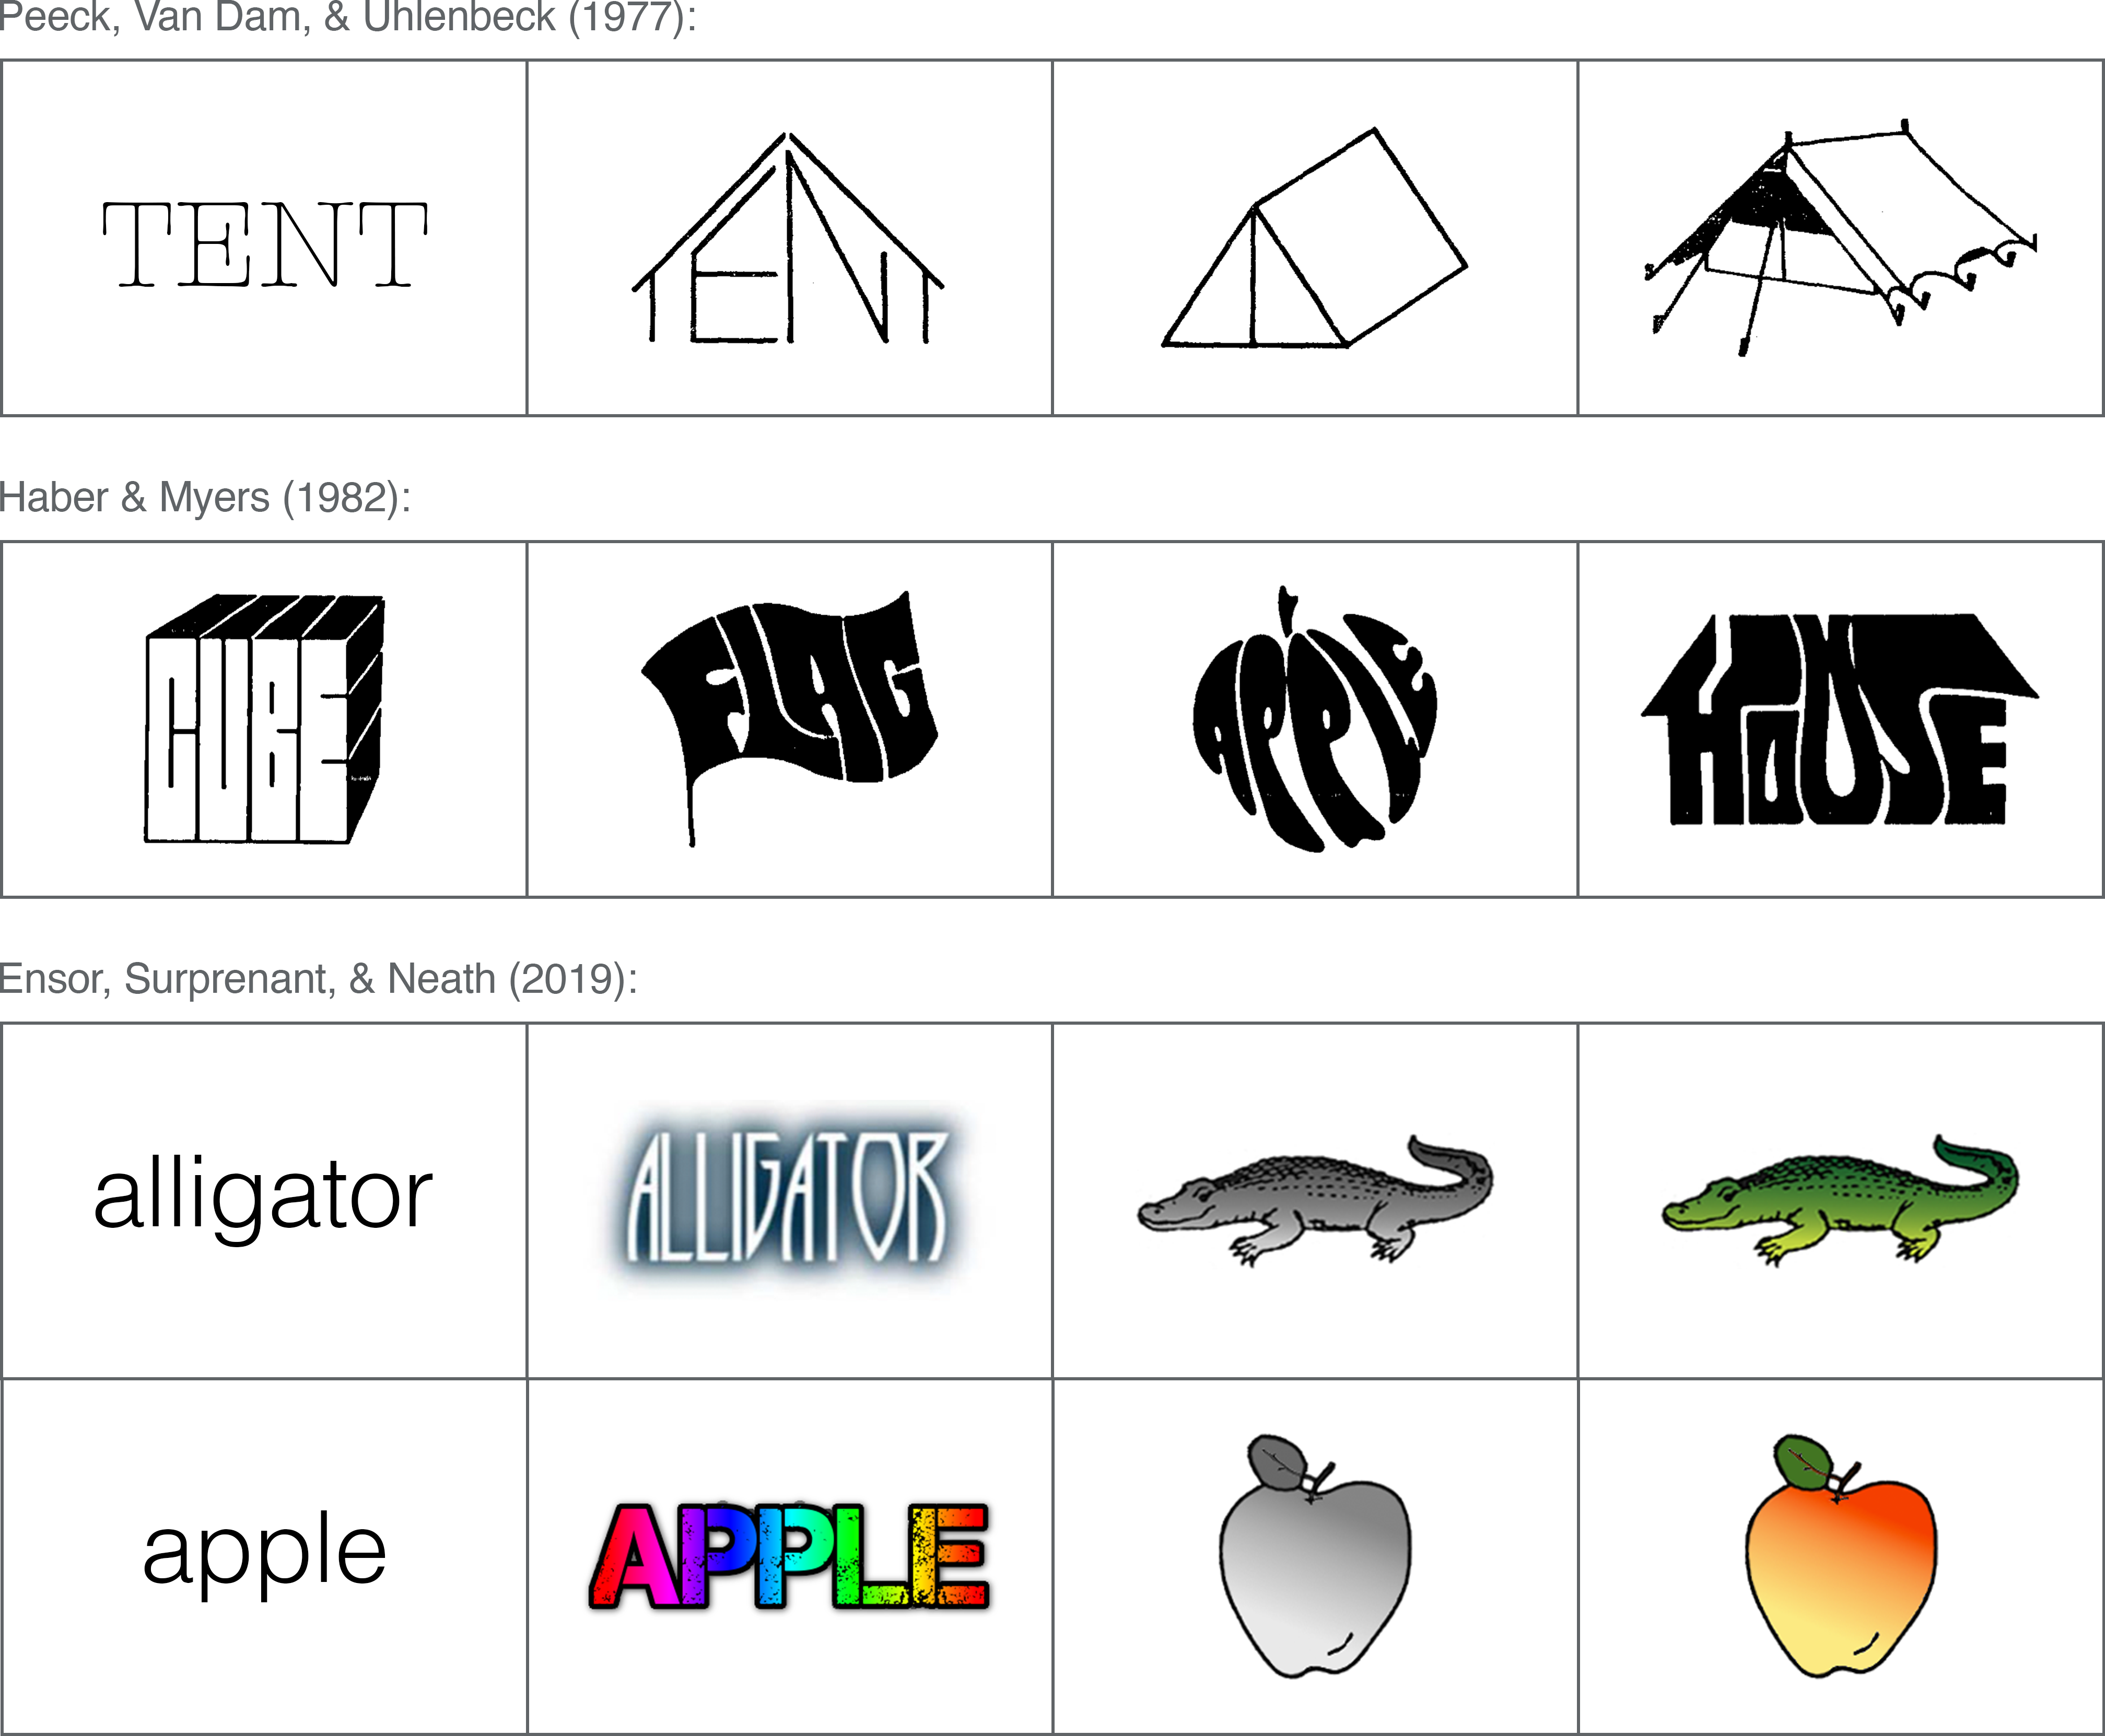
\includegraphics[width=1\linewidth]{./resources/images/exp5__background_stim_examples} \end{center}

Figure 21: Example stimuli taken from Peeck et al. (1977), Haber \&
Myers (1982), and Ensor et al. (2019).

More recent work has examined the manipulation of word distinctiveness
in recognition memory paradigms. In a effort to disentangle the
prevalent theories of the PSE, Ensor et al. (2019) increased the
item-to-item variability of word stimuli by utilising unique typefaces,
a range of colour combinations, inconsistent sizes, and selective use of
capitalisation (see Figure 21 for example items). In recognition memory
paradigms, word stimuli are typically presented in a plain black,
readable typeface (e.g.~Arial, Times), with a focus on consistency
between items (i.e.~aside from the word itself, all other variables are
often equal); the manipulation by Ensor et al. (2019) increased the
variability across items under the assumption distinctiveness would be
enhanced. Comparing recognition memory performance for such items
against regular words and pictures produces some distinct and
contrasting predictions. Operating under the physical distinctiveness
account of the PSE, recognition should be enhanced for the more-distinct
word stimuli in comparison to regular word stimuli; as such, when
comparing these items with pictures, PSEs should be reduced or even
eliminated as the differences in distinctiveness that drive the PSE are
lessened. DCT, on the other hand, predicts no elimination of the PSE;
manipulations to the colour, font, and capitalisation of word stimuli do
nothing to negate the additional imagery code that is readily available
for pictures. Thus, pictures will continue to show memorial advantages
irrespective of how word stimuli - constrained by a single, verbal code
- are presented. Recognition performance was compared in an old new
paradigm for low distinctive words (black, plain font), high distinctive
words (varying fonts, colours, size, and capitalisation), low
distinctive pictures (greyscale drawings) and high distinctive pictures
(colour drawings). Results showed that, while a standard PSE was
observed between greyscale pictures and black words, there was no PSE
between greyscale pictures and colour words, indicating the formats were
similarly memorable as a result of the manipulation. The colour word
stimuli were also shown to attenuate the PSE when comparisons were made
with colour pictures, and when trial numbers were increased, the PSE was
eliminated here too. Such findings offer convincing support for the
physical distinctiveness account, in that increasing the distinctiveness
of word stimuli acts to eliminate picture superiority. As such, it is
difficult to reconcile these results in a dual-coding framework, which
predicts any word items to consistently show diminished performance
compared to pictures.

The current study has two primary aims: i) replicate the elimination of
the PSE demonstrated by Ensor et al. (2019); ii) examine whether the
PhSE is also attenuated / eliminated when comparing photograph items
with distinctive word stimuli. A secondary aim is to further
characterise the role of colour in the previously established
\emph{photo} superiority effect (PhSE). Since previous analyses could
only be performed between drawings and photographs of the same colour
modality (i.e.~i) drawings without vs.~photographs without in
\emph{Experiment 3}; and ii) drawings with vs.~photographs with in
\emph{Experiment 4}), the extent to which colour is involved in the
PhSE, if at all, remains mostly unclear. In a scene recognition paradigm
(utilising pictures of city streets, parks etc.), Suzuki \& Takahashi
(1997) demonstrated enhanced recognition performance when colour - as
opposed to greyscale - items were shown at study and test.
Interestingly, this benefit was only apparent when study and test
conditions congruently presented items in colour; any recognition
enhancements attributed to colour disappeared when blocks were
incongruent (e.g.~items presented in grey at study, and the same items
presented in colour at test). Suzuki \& Takahashi (1997) also found that
subjects' memory for the colour mode they had seen items in at study was
poor; in other words, participants could not remember well whether they
had studied items in colour or greyscale, despite exhibiting better
recognition for congruent colour items. Since the benefits of colour
information could not be attributed to any conscious recall of the
actual colours in the pictures, it was instead hypothesised colour
information acts to indirectly highlight certain features in a picture -
i.e.~details that were not otherwise noticed as prominently in greyscale
- and thus increases their distinctiveness (and memorability) as a
result. It is unclear whether colour information provides similar
benefits in object recognition, or if this effect applies exclusively to
real-world photographs of scenes (presumably comprised of a multitude of
items).

If colour enhancements akin to those demonstrated by Suzuki \& Takahashi
(1997) are indeed also present in object recognition, it is possible
that the PhSE could be eliminated as a result. In the same way the PSE
is eliminated between words and drawings when word stimuli are made more
distinctive (Ensor et al., 2019), the PhSE may too be eliminated when
comparisons are made between colour drawings (whose distinctiveness is
presumably somewhat enhanced by colour) and greyscale photographs (whose
real-world details and textures increase their distinctiveness in
relation to drawings, but colour enhancements are absent). Indeed, there
is some evidence to support this notion; the normative data obtained by
Rossion \& Pourtois (2004) for their revised set of Snodgrass \&
Vanderwart (1980) object drawings revealed clear object naming benefits
when items were presented in colour. When subjects were asked to provide
single-word, unambiguous labels toward a number of illustrated object
stimuli, naming agreement scores across participants were significantly
higher for items presented in colour, as opposed to illustrations shown
in greyscale (and simple un-shaded outlines). Reaction times were also
significantly faster for the colour items compared to the other types.
While these effects were most pronounced when items had a diagnostic
colour (e.g.~fruits), items depicting man-made objects without
diagnostic colours also showed such benefits. The researchers concluded
colour information clearly plays a role in facilitating basic everyday
item recognition, however, similar benefits are not consistently
supported in other experimental paradigms involving memory. In a free
recall task, Paivio et al. (1968) compared PSE effects for greyscale and
colour items and found no effect of colour - in fact, recall was
generally poorer for the colour items. In a recognition memory paradigm,
Ensor et al. (2019) demonstrated some minor differential effects of
colour; in their first experiment, an elimination of the PSE was
demonstrated when their distinctive words were compared with
\emph{greyscale} drawings (suggesting both formats exhibited similar
levels of distinctiveness), but the PSE was only attenuated when their
distinctive words were compared with \emph{colour} drawings (suggesting
the colour drawings were presumably more distinct than the greyscale
drawings). However, this minor benefit of colour information disappeared
when the number of study and test trials were doubled, as the PSE was
then eliminated for greyscale \emph{and} colour drawings.

It may be that any distinctiveness benefits afforded by colour are
particularly susceptible to methodological circumstances, or indeed are
simply negligible - a notion supported thus far in the current programme
of research. Visual inspection of the results from \emph{Experiment 3}
(greyscale pictures) and \emph{Experiment 4} (colour pictures) suggest
no enhancements as a result of colour information with both presentation
types displaying highly similar PSE and PhSE magnitudes, proportions of
hits, FAs, and mean \emph{d'} scores, and patterns of RFG responding. As
photographs were consistently recognised better than drawings, however,
we cannot interpret the lack of a colour enhancement as evidence of DCT
in the same was as Paivio et al. (1968). Rather, the findings instead
characterise colour as a factor that does not contribute to the physical
distinctiveness of an object, contrary to what we might assume. An
elimination of the PhSE therefore seems unlikely; if colour information
shows no discernible benefit in recognition memory paradigms,
performance toward greyscale photographs will likely remain superior in
comparison to colour drawings.

Based on results of the previous experiments, and the research discussed
above, the following hypotheses are proposed:

\begin{enumerate}
\def\labelenumi{\arabic{enumi}.}
\tightlist
\item
  Recognition will be enhanced for word stimuli characterised by
  distinct variations to colour, font, and capitalisation across items,
  compared to those consistently presented in the same black typeface.
  For colour words, this enhancement is expected to manifest as the
  following compared to greyscale words:

  \begin{itemize}
  \item
    \begin{enumerate}
    \def\labelenumii{\roman{enumii})}
    \tightlist
    \item
      higher overall \emph{d'} scores;
    \end{enumerate}
  \item
    \begin{enumerate}
    \def\labelenumii{\roman{enumii})}
    \setcounter{enumii}{1}
    \tightlist
    \item
      higher proportion of correct hits;
    \end{enumerate}
  \item
    \begin{enumerate}
    \def\labelenumii{\roman{enumii})}
    \setcounter{enumii}{2}
    \tightlist
    \item
      lower proportion of false alarms.
    \end{enumerate}
  \end{itemize}
\end{enumerate}

Such findings will establish a successful replication of the Ensor et
al. (2019) manipulation, and allow for the examination of PSE
elimination effects in the current paradigm.

\begin{enumerate}
\def\labelenumi{\arabic{enumi}.}
\setcounter{enumi}{1}
\item
  A picture superiority effect (PSE) will be evident, whereby
  recognition for either picture type (drawings / photographs) will be
  enhanced in comparison to greyscale words. Drawings and photographs
  are expected to show the same performance benefits as above compared
  to greyscale words.
\item
  PSEs will be eliminated when recognition is compared for colour words
  and shaded drawings:

  \begin{itemize}
  \tightlist
  \item
    Elimination of the PSE when colour words are compared with greyscale
    drawings;
  \item
    Attenuation or elimination of the PSE when colour words are compared
    with colour drawings.
  \end{itemize}
\end{enumerate}

Ensor et al. (2019) observed differences in the comparison between
colour words and colour drawings, depending upon the number of trials
presented to participants (attenuation: 40 trials at study + 80 at test;
elimination: 80 trials at study + 160 at test). As the current study is
situated between these (60 trials at study + 120 at test), either
outcome is expected.

\begin{enumerate}
\def\labelenumi{\arabic{enumi}.}
\setcounter{enumi}{3}
\tightlist
\item
  A \emph{photograph} superiority effect (PhSE) will also be apparent:

  \begin{itemize}
  \tightlist
  \item
    Greyscale photographs will produce better recognition than greyscale
    drawings (as in \emph{Experiment 3});
  \item
    Colour photographs will produce better recognition than colour
    drawings (as in \emph{Experiment 4});
  \item
    Greyscale photographs will produce better recognition than colour
    drawings (the PhSE will not be eliminated when drawings are shown in
    colour).
  \end{itemize}
\item
  PSEs between colour words and photographs will persist:

  \begin{itemize}
  \tightlist
  \item
    While the recognition benefits afforded to colour words may
    eliminate or attenuate the PSE when comparisons are made with
    drawing stimuli, this will not be sufficient to eliminate the effect
    when comparisons are made with photographs.
  \end{itemize}
\end{enumerate}

\hypertarget{experiment-manipulating-word-distinctiveness}{%
\subsection{Experiment: Manipulating word
distinctiveness}\label{experiment-manipulating-word-distinctiveness}}

\hypertarget{method-4}{%
\subsubsection{Method}\label{method-4}}

\hypertarget{participants-4}{%
\paragraph{Participants}\label{participants-4}}

\hfill\break A total of 173 participants completed the online
experiment, all between the ages 18-59 years (see Table 11 for a
breakdown of the age/gender of the current sample). The majority of
participants reported English as being their first language (87.86\%).
Participants were primarily recruited from the in-house
research participation system\footnote{\url{https://keelepsychology.sona-systems.com/}}
(91.33\%), though some were also sourced from the voluntary
participation website
Prolific Academic\footnote{\url{https://www.prolific.co/}} (4.05\%),
where payment at the rate of £5/hr was given, and from other online
social media (e.g.~Facebook; 4.62\%). Sample size was calculated
a-priori using
G*Power\footnote{\url{https://www.psychologie.hhu.de/arbeitsgruppen/allgemeine-psychologie-und-arbeitspsychologie/gpower}}
(Faul, Erdfelder, Buchner, \& Lang, 2009) to detect a small effect size
of Cohen's \emph{f} = 0.1 with 95\% power (\emph{α} = .05, two-tailed),
166 subjects would be necessary in a one-way repeated measures ANOVA.

~ ~

Table 11: Gender and age (\emph{SD}) of the current sample.

\begin{table}[!h]
\centering
\begin{tabular}{l>{}rr>{}l}
\toprule
Gender & N & Age & (SD)\\
\midrule
Female & \em{139} & 20.63 & \em{(6.09)}\\
Male & \em{31} & 21.26 & \em{(7.97)}\\
Female/Non-binary & \em{1} & 19.00 & \em{(0)}\\
FTM Transgender & \em{1} & 23.00 & \em{(0)}\\
Unspecified & \em{1} & 32.00 & \em{(0)}\\
\addlinespace
\textbf{Total} & \textbf{\em{173}} & \textbf{20.81} & \textbf{\em{(6.46)}}\\
\bottomrule
\end{tabular}
\end{table}

\hypertarget{materials-4}{%
\paragraph{Materials}\label{materials-4}}

\hfill\break Three stimuli formats were utilised in the current
experiment - words, drawings, and photographs - each of which had colour
and greyscale variations (see Figure 22 for example stimuli). Shaded
drawings were sourced from Rossion and Pourtois (2004) and consisted of
shaded illustrations of innocuous, everyday objects (e.g.~clock, rabbit,
shoe). The photographs were those curated in \emph{Experiment 2} - high
quality photographs that similarly depicted the same everyday objects as
those found in the Rossion \& Pourtois (2004) drawings, with the objects
of interest isolated from their original backgrounds. Word stimuli
consisted of the written-word labels for each of the objects; the
greyscale word stimuli consisted of a simple sans-serif typeface (Roboto
light; 54pt) presented in plain black ink, while the colour variations
contained manipulations to font, size, colour, and capitalisation. In
their experiment, Ensor et al. (2019) made comparisons to the same set
of drawings used in the current study; as such, many of their colour
word items could be re-purposed for use in the current study. However,
as not \emph{all} of the current pool of items were represented in this
previous experiment, new colour word items were also created using the
same design source
(Cool Text Graphics Generator\footnote{\url{https://cooltext.com/}}).
Every effort was made to match the font styles of the newly created
words (i.e.~objects that had not been present in the Ensor et al. (2019)
study) with those that had been utilised previously for different
objects. All stimuli were separately placed on a 500x500px blank canvas
using Adobe Photoshop 2021 (22.0.0 Release); some items were constrained
to this canvas size by their height, while others were constrained by
their width, depending on the dimensions of the object. All items were
exported as .pngs files for presentation by the online survey platform,
where they were presented at their actual size (i.e.~without scaling) to
ensure consistency across participants.

\hypertarget{design-4}{%
\paragraph{Design}\label{design-4}}

\hfill\break A one-way repeated measures design was utilised, consisting
of a within-subjects factor of stimuli format with six levels: i)
greyscale words; ii) colour words; iii) greyscale drawings; iv) colour
drawings; v) greyscale photographs; vi) colour photographs. Participants
completed a single study block (60 items) and a single test block (120
items), both of which were comprised of an equal number of items for
each of the six stimuli formats. The particular format objects were
presented in (for example, whether the item ``penguin'' was presented as
a colour word or as a greyscale photograph) was counterbalanced across
participants via blocked randomisation. All study / test
counterbalancing routes were of equal length.

~ ~

\begin{center}\includegraphics[width=0.74\linewidth]{./resources/images/exp5__stim_examples} \end{center}

Figure 22: Examples of the six stimuli formats utilised in the current
experiment: greyscale and colour variations of words, drawings, and
photographs.

\hypertarget{procedure-4}{%
\paragraph{Procedure}\label{procedure-4}}

\hfill\break As in previous experiments, data was collected online using
the Gorilla\footnote{\url{https://gorilla.sc/}} experiment platform.
Participants completed three self-paced phases: i) study phase, ii)
distractor task, and iii) recognition test. In the study phase, subjects
were instructed to learn each of the items presented in preparation for
a later memory test. Word, drawing, and photograph items were displayed
one-at-a-time at random on-screen, and for each subjects required to
report whether the current format was a word, drawing, or photograph. No
distinction was made between greyscale and colour items in the wording
of these response options (i.e.~participants should respond ``Word'' to
greyscale words \emph{and} colour words), since this encoding judgement
was utilised simply to ensure subjects directed their attention toward
the to-be-remembered stimuli. Following the study phase, subjects
completed a distractor task consisting of simple multiple choice
mathematical questions (e.g.~6 x 4 = ?), before finally being presented
with the recognition test. Subjects were again presented with items from
each of the six stimuli formats. shown one-at-a-time at random
on-screen. While half of the test items had been presented earlier in
the study phase, the other half were new and had not been studied.
First, subjects were first required to make \emph{Old}/\emph{New}
judgements based on whether they recognised each of the items. If
subjects experienced no recognition toward an item (and thus selected
\emph{New}) they would simply continue to the next item. If subjects did
experience recognition (and thus selected \emph{Old}), they were
presented with a follow-up screen probing how they had arrived at this
decision; subjects were asked to report whether they had recognised the
item via \emph{Recollection}, \emph{Familiarity}, or were simply
\emph{Guessing} that it was old. Within participants, the format items
were presented in remained the same across study and test (e.g.~if the
item ``penguin'' was shown in grey word format at study, it was also
shown as a grey word at test).

\hypertarget{data-processing-4}{%
\paragraph{Data processing}\label{data-processing-4}}

\hfill\break Subjects were excluded from analyses on the basis of two
key criteria; 1) less than 90\% accuracy during the encoding task
(\emph{N}= 14; where they were asked to report whether each item was
shown as a word, drawing, or photograph); 2) extreme z-scores (\emph{N}=
1; i.e.~those presenting z-scores of +/- 3 for total hits, total FAs, or
overall recognition {[}hits minus FAs{]}).The subjects to meet these
criteria were considered outliers and excluded from analysis, leaving a
total of 158 datasets.

The primary DVs of interest consisted of the mean proportion of hits and
false alarms (FAs), mean \emph{d'} scores (d-prime, a signal detection
measure of sensitivity), and the total number of hits and FAs assigned
\emph{Recollection}, \emph{Familiarity}, and \emph{Guessing}.
Comparisons are made in relation to the first two experiments of Ensor
et al. (2019), the methodologies of which were identical to one another,
apart from the number of trials involved (one experiment consisting of
40 trials at study and 80 at test, and the other consisting of 80 trials
at study and 160 at test). With regard to trial numbers, the current
study sits between the two Ensor et al. (2019) experiments, with 60
trials at study and 120 at test. All analyses were conducted with
\emph{R} (R Core Team, 2020) using the \emph{afex} (v0.28-0; Singmann et
al., 2020) and \emph{rstatix} packages (v0.6.0; Kassambara, 2020).

\hypertarget{results-4}{%
\subsubsection{Results}\label{results-4}}

To address each of the hypotheses, a series of one-way repeated measures
analyses of variance (ANOVA) - using six factors (grey \& distinctive
words, grey \& colour drawings, grey \& colour photographs) - were
conducted on the mean proportions of hits, mean proportion of FAs, and
mean \emph{d'}scores. Sphericity was assessed using Mauchly's Test; when
the assumption of sphericity was violated, Greenhouse-Geisser
corrections were applied.

To compare the results of the current study with previous findings, the
raw data from the first two experiments of Ensor et al. (2019) was
re-analysed in order to calculate statistics that were not reported in
their paper.

\newpage

\hypertarget{picture-superiority-pse}{%
\paragraph{Picture superiority (PSE)}\label{picture-superiority-pse}}

Standard PSEs were apparent in the ANOVAs on the mean proportion of
hits, mean proportion of FAs, and mean \emph{d'} scores. Grey words
(\emph{M} = 0.58) showed a significantly lower proportion of hits
compared to all types of picture: grey drawings (\emph{M} = 0.75),
\emph{t}(157) = 9.04, \emph{p} \textless{} .001, \emph{d} = 0.72; grey
photographs (\emph{M} = 0.91), \emph{t}(157) = 17.42, \emph{p}
\textless{} .001, \emph{d} = 1.39; colour drawings (\emph{M} = 0.78),
\emph{t}(157) = 10.37, \emph{p} \textless{} .001, \emph{d} = 0.83; and
colour photographs (\emph{M} = 0.91), \emph{t}(157) = 17.53, \emph{p}
\textless{} .001, \emph{d} = 1.39. Grey words (\emph{M} = 0.18) also
showed a significantly higher proportion of FAs compared to all types of
picture: grey drawings (\emph{M} = 0.08), \emph{t}(157) = -6.60,
\emph{p} \textless{} .001, \emph{d} = -0.52; grey photographs (\emph{M}
= 0.04), \emph{t}(157) = -9.31, \emph{p} \textless{} .001, \emph{d} =
-0.74; colour drawings (\emph{M} = 0.05), \emph{t}(157) = -8.45,
\emph{p} \textless{} .001, \emph{d} = -0.67; and colour photographs
(\emph{M} = 0.02), \emph{t}(157) = -10.72, \emph{p} \textless{} .001,
\emph{d} = -0.85. Finally, mean \emph{d'} scores were also significantly
lower for grey words (\emph{M} = 1.49) compared to all types of picture:
grey drawings (\emph{M} = 2.65), \emph{t}(157) = 12.37, \emph{p}
\textless{} .001, \emph{d} = 0.98; grey photographs (\emph{M} = 3.62),
\emph{t}(157) = 24.28, \emph{p} \textless{} .001, \emph{d} = 1.93;
colour drawings (\emph{M} = 2.89), \emph{t}(157) = 14.80, \emph{p}
\textless{} .001, \emph{d} = 1.18; and colour photographs (\emph{M} =
3.83), \emph{t}(157) = 24.61, \emph{p} \textless{} .001, \emph{d} =
1.96.

\newpage

\hypertarget{photograph-superiority-phse}{%
\paragraph{Photograph superiority
(PhSE)}\label{photograph-superiority-phse}}

Examining greyscale items only, a PhSE was apparent across each of the
variables (as demonstrated previously in \emph{Experiment 3}). Grey
photographs (\emph{M} = 0.91) showed a significantly higher proportion
of hits compared to grey drawings (\emph{M} = 0.75), \emph{t}(157) =
-10.75, \emph{p} \textless{} .001, \emph{d} = -0.86; grey photographs
(\emph{M} = 0.04) showed a significantly lower proportion of FAs
compared to grey drawings (\emph{M} = 0.08), \emph{t}(157) = 3.86,
\emph{p} \textless{} .001, \emph{d} = 0.31; and grey photographs
(\emph{M} = 3.62) showed significantly higher mean \emph{d'} scores than
grey drawings (\emph{M} = 2.65), \emph{t}(157) = -11.37, \emph{p}
\textless{} .001, \emph{d} = -0.90. Examining colour items only, a PhSE
was similarly apparent across each of the variables (as demonstrated
previously in \emph{Experiment 4}). Colour photographs (\emph{M} = 0.91)
showed a significantly higher proportion of hits compared to colour
drawings (\emph{M} = 0.78), \emph{t}(157) = -10.03, \emph{p} \textless{}
.001, \emph{d} = -0.80; colour photographs (\emph{M} = 0.02) showed a
significantly lower proportion of FAs compared to colour drawings
(\emph{M} = 0.05), \emph{t}(157) = 4.57, \emph{p} \textless{} .001,
\emph{d} = 0.36; and colour photographs (\emph{M} = 3.83) showed
significantly higher mean \emph{d'} scores than colour drawings
(\emph{M} = 2.89), \emph{t}(157) = -10.81, \emph{p} \textless{} .001,
\emph{d} = -0.86.

To examine the role of colour vs.~greyscale in the PhSE, colour drawings
were compared with greyscale photographs to examine whether the PhSE was
eliminated. Colour drawings (\emph{M} = 0.78) showed a significantly
lower proportion of hits compared to grey photographs (\emph{M} = 0.91),
\emph{t}(157) = -9.62, \emph{p} \textless{} .001, \emph{d} = -0.77.
Colour drawings also (\emph{M} = 2.89) showed a significantly lower mean
\emph{d'} scores compared to grey photographs (\emph{M} = 3.62),
\emph{t}(157) = -7.51, \emph{p} \textless{} .001, \emph{d} = -0.60.
However, the PhSE was eliminated when comparing colour drawings
(\emph{M} = 0.05) and grey photographs (\emph{M} = 0.04) on the mean
proportion of FAs, where there was no difference between the formats,
\emph{t}(157) = 1.74, \emph{p} = .083, \emph{d} = 0.14.

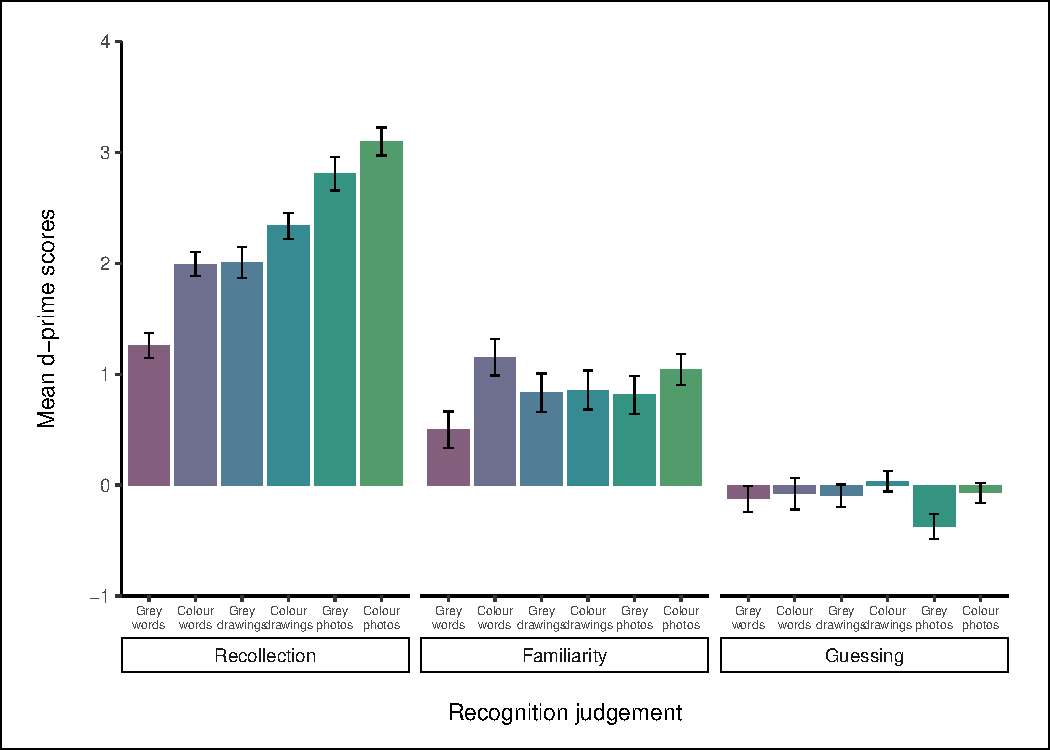
\includegraphics{R--Thesis_files/figure-latex/unnamed-chunk-81-1.pdf}
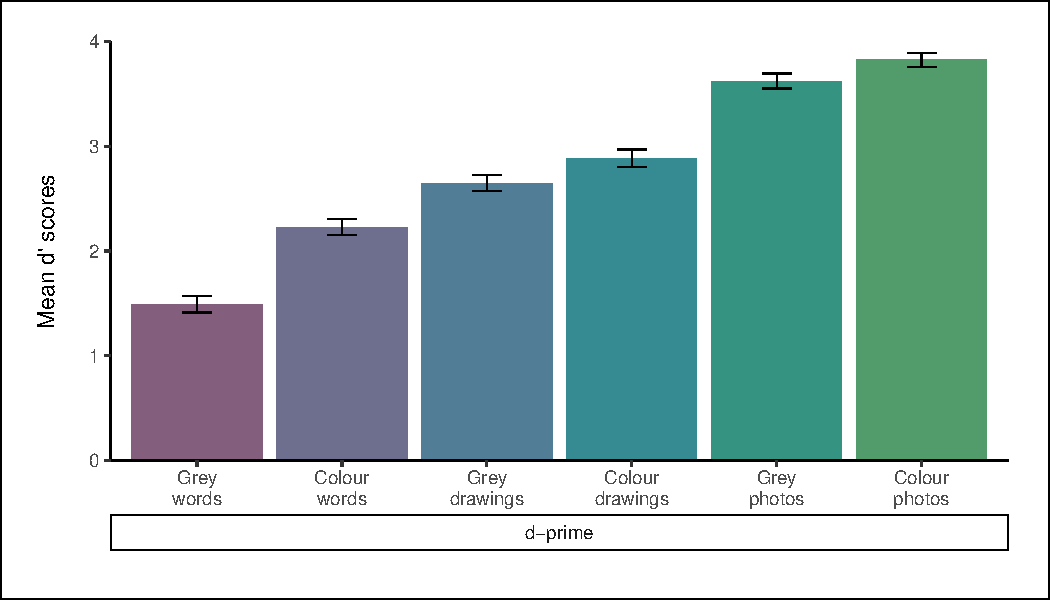
\includegraphics{R--Thesis_files/figure-latex/unnamed-chunk-81-2.pdf}
Figure 23: Mean proportion of hits, FAs, and d' scores by stimuli
format.

\newpage

\hypertarget{manipulation-check}{%
\paragraph{Manipulation check}\label{manipulation-check}}

Throughout each of the conducted ANOVAs, there was consistently a
significant main effect of stimuli format: mean proportion of hits
{[}\emph{F}(3.95, 619.49) = 137.94, \emph{p} \textless{} .001,
\(\eta^2_p\) = .47{]}, mean proportion of FAs {[}\emph{F}(2.83, 443.69)
= 52.71, \emph{p} \textless{} .001, \(\eta^2_p\) = .25{]}, mean
\emph{d'}-scores {[}\emph{F}(4.74, 744.81) = 190.22, \emph{p}
\textless{} .001, \(\eta^2_p\) = .55{]}. Planned comparisons following
these significant results, however, did not always demonstrate that the
distinctive word stimuli were indeed any more distinctive than the
regular word stimuli. Primarily, there was no difference in the
proportion of overall hits between distinctive (\emph{M} = 0.61) and
regular words (\emph{M} = 0.58), \emph{t}(157) = 1.26, \emph{p} = .211,
\emph{d} = 0.10 - recognition performance (i.e.~the number of items
subjects were able to correctly identify) was the same regardless of the
format word stimuli were presented in. Subjects did, however, make
significantly fewer FAs as a result of the manipulation (distinctive
words \emph{M} = 0.05, regular words \emph{M} = 0.18; \emph{t}(157) =
-8.70, \emph{p} \textless{} .001, \emph{d} = -0.69), offering some
support to the manipulation, as subjects were better able to correctly
reject lure items when they were presented in a distinctive format,
rather than regular format, highlighting some performance benefits.
Furthermore, distinctive words (\emph{M} = 2.23) also showed
significantly higher \emph{d'} scores than regular words (\emph{M} =
1.49), \emph{t}(157) = 7.96, \emph{p} \textless{} .001, \emph{d} = 0.63;
subjects were better able to accurately discriminate between hits and
FAs when responding to the distinctive words over regular words.

\begin{verbatim}
## Warning: Use of `exp5__figure__rfg.hits.data$ymin` is discouraged. Use `ymin`
## instead.
\end{verbatim}

\begin{verbatim}
## Warning: Use of `exp5__figure__rfg.hits.data$ymax` is discouraged. Use `ymax`
## instead.
\end{verbatim}

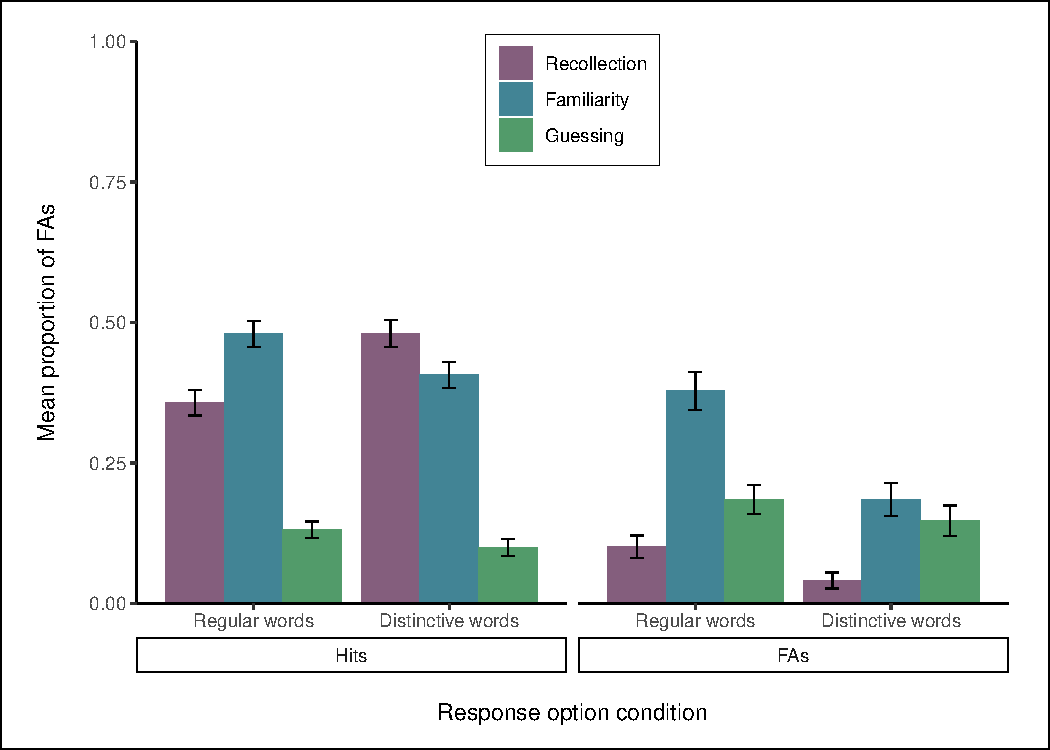
\includegraphics{R--Thesis_files/figure-latex/unnamed-chunk-83-1.pdf}
Figure 24: Mean proportion of hits and FAs assigned Recollection,
Familiarity, and Guessing by stimuli format.

Analysis of the Ensor et al. (2019) data showed evidence of the
distinctiveness manipulation. For the mean proportion of hits, there
were significant main effects of stimuli format in their first
{[}\emph{F}(3, 87) = 10.91, \emph{p} \textless{} .001, \(\eta^2_p\) =
.27{]} and second {[}\emph{F}(3, 87) = 8.37, \emph{p} \textless{} .001,
\(\eta^2_p\) = .22{]} experiments. Follow-up comparisons showed
distinctive words resulted in significantly more hits than regular words
across both experiments (see Table 13). For the mean proportion of FAs,
the first experiment of Ensor et al. (2019) showed no significant main
effect of stimuli format {[}\emph{F}(3, 87) = 1.41, \emph{p} = .245,
\(\eta^2_p\) = .05{]}, however, the second experiment did {[}\emph{F}(3,
87) = 6.05, \emph{p} \textless{} .001, \(\eta^2_p\) = .17{]}; though
follow-up comparisons showed no difference in the proportion of FAs
between distinctive and regular words. Finally, for mean \emph{d'}
scores, there was a significant main effect of stimuli format in both
the first {[}\emph{F}(3, 87) = 10.99, \emph{p} \textless{} .001,
\(\eta^2_p\) = .27{]} and second {[}\emph{F}(3, 87) = 19.01, \emph{p}
\textless{} .001, \(\eta^2_p\) = .40{]} experiments. Follow-up
comparisons showed evidence of the distinctiveness manipulation, whereby
distinctive words produced significantly higher \emph{d'} scores
compared to regular words in both experiments (see Table 12).

~

Table 12: Mean proportion of hits for regular and distinctive word
stimuli, across the current experiment and Ensor et al. (2019).

\begin{verbatim}
## Usually it is recommended to use column_spec before collapse_rows, especially in LaTeX, to get a desired result.
\end{verbatim}

\begingroup\fontsize{10}{12}\selectfont

\begin{tabu} to \linewidth {>{\raggedleft\arraybackslash}p{2cm}>{\raggedright}X>{\centering}X>{\centering}X>{\raggedright}X}
\toprule
  &    & Grey words & Distinctive words & Planned comparisons\\
\midrule
\addlinespace[0.3em]
\multicolumn{5}{l}{\textbf{Hits}}\\
\textbf{\hspace{1em}} & Trials: 40 study / 80 test: & 0.72 & 0.84 & *t*(29) = 3.14, *p* = .004, *d* = 0.57\\
\cmidrule{2-5}
\textbf{\hspace{1em}\multirow[t]{-2}{*}{\raggedleft\arraybackslash Ensor, Surprenant, \& Neath (2019)}} & Trials: 80 study / 160 test: & 0.63 & 0.78 & *t*(29) = 4.16, *p* < .001, *d* = 0.76\\
\cmidrule{1-5}
\textbf{\hspace{1em}Current study} & Trials: 60 study / 120 test: & 0.58 & 0.61 & *t*(157) = 1.26, *p* = .211, *d* = 0.10\\
\cmidrule{1-5}
\addlinespace[0.3em]
\multicolumn{5}{l}{\textbf{FAs}}\\
\textbf{\hspace{1em}} & Trials: 40 study / 80 test: & 0.15 & 0.08 & *t*(29) = -1.94, *p* = .062, *d* = -0.35\\
\cmidrule{2-5}
\textbf{\hspace{1em}\multirow[t]{-2}{*}{\raggedleft\arraybackslash Ensor, Surprenant, \& Neath (2019)}} & Trials: 80 study / 160 test: & 0.29 & 0.23 & *t*(29) = -1.48, *p* = .149, *d* = -0.27\\
\cmidrule{1-5}
\textbf{\hspace{1em}Current study} & Trials: 60 study / 120 test: & 0.18 & 0.05 & *t*(157) = -8.70, *p* < .001, *d* = -0.69\\
\cmidrule{1-5}
\addlinespace[0.3em]
\multicolumn{5}{l}{\textbf{d'}}\\
\textbf{\hspace{1em}} & Trials: 40 study / 80 test: & 2.18 & 2.97 & *t*(29) = 3.69, *p* < .001, *d* = 0.67\\
\cmidrule{2-5}
\textbf{\hspace{1em}\multirow[t]{-2}{*}{\raggedleft\arraybackslash Ensor, Surprenant, \& Neath (2019)}} & Trials: 80 study / 160 test: & 1.09 & 1.89 & *t*(29) = 7.35, *p* < .001, *d* = 1.34\\
\cmidrule{1-5}
\textbf{\hspace{1em}Current study} & Trials: 60 study / 120 test: & 1.49 & 2.23 & *t*(157) = 7.96, *p* < .001, *d* = 0.63\\
\bottomrule
\end{tabu}
\endgroup{}

\newpage

\hypertarget{elimination-of-pse-comparison-with-ensor2019b}{%
\paragraph{Elimination of PSE (comparison with Ensor et al.
(2019))}\label{elimination-of-pse-comparison-with-ensor2019b}}

A key finding in Ensor et al. (2019) data was an elimination of the PSE;
distinctive word stimuli and grey drawings produced similar \emph{d'}
scores, indicative of comparable distinctiveness between the two stimuli
formats. Such findings were replicated in the current reanalysis of
their data (see Table 14). In the current experiment, however, this
finding was not replicated, with drawings showing significantly higher
\emph{d'} than the distinctive words, suggesting the manipulation was
not effective.

Similarly, Ensor et al. (2019) also showed no difference in the number
of hits between the distinctive words and grey drawings, across both
experiments. This again suggests their distinctiveness manipulation was
successful in eliminating the PSE, however, such a finding was not
apparent in the current study, where grey drawings produced
significantly more hits than the distinctive words.

Finally, Ensor et al. (2019) also showed no difference in the number of
FAs between the distinctive words and grey drawings, across both
experiments - an expected result if the distinctiveness manipulation
resulted in similar levels between the distinctive words and grey
drawings. Again, the current experiment produced different results;
interestingly though, there were significantly more FAs for the grey
drawings, as opposed to the distinctive word stimuli. This is somewhat
unexpected, since the rest of the findings identify the grey drawings as
having increased memorability compared to the distinctive words.

Table 14: Mean \emph{d;} scores for distinctive word stimuli and grey
drawings, across the current experiment and Ensor et al. (2019).
\begingroup\fontsize{10}{12}\selectfont

\begin{tabu} to \linewidth {>{\raggedleft}X>{\centering\arraybackslash}p{1.2cm}>{\centering\arraybackslash}p{1.2cm}>{\centering\arraybackslash}p{6cm}>{\raggedleft}X}
\toprule
\multicolumn{1}{c}{\textbf{ }} & \multicolumn{3}{c}{\textbf{*d'}} \\
\cmidrule(l{3pt}r{3pt}){2-4}
\hspace{1em}  &    & Distinctive words & Grey drawings & Planned comparisons\\
\midrule
\addlinespace[0.3em]
\multicolumn{5}{l}{\textbf{Ensor, Surprenant, \& Neath (2019)}}\\
\hspace{1em}\hspace{1em}Ensor, Surprenant, & Neath (2019) & Trials: 40 study / 80 test: & 0.84 & 0.86 & *t*(29) = -0.69, *p* = .495, *d* = -0.13\\
\hspace{1em}\hspace{1em}Ensor, Surprenant, & Neath (2019) & Trials: 80 study / 160 test: & 0.78 & 0.75 & *t*(29) = 0.98, *p* = .333, *d* = 0.18\\
\addlinespace[0.3em]
\multicolumn{5}{l}{\textbf{Current study}}\\
\hspace{1em}Current study & Trials: 60 study / 120 test: & 0.61 & 0.75 & *t*(157) = -7.28, *p* < .001, *d* = -0.58\\
Ensor, Surprenant, & Neath (2019) & Trials: 40 study / 80 test: & 0.08 & 0.12 & *t*(29) = -1.38, *p* = .178, *d* = -0.25\\
Ensor, Surprenant, & Neath (2019) & Trials: 80 study / 160 test: & 0.23 & 0.19 & *t*(29) = 1.06, *p* = .297, *d* = 0.19\\
Current study & Trials: 60 study / 120 test: & 0.05 & 0.08 & *t*(157) = -2.48, *p* = .014, *d* = -0.20\\
Ensor, Surprenant, & Neath (2019) & Trials: 40 study / 80 test: & 2.97 & 2.96 & *t*(29) = 0.06, *p* = .956, *d* = 0.01\\
Ensor, Surprenant, & Neath (2019) & Trials: 80 study / 160 test: & 1.89 & 1.90 & *t*(29) = -0.07, *p* = .945, *d* = -0.01\\
Current study & Trials: 60 study / 120 test: & 2.23 & 2.65 & *t*(157) = -4.70, *p* < .001, *d* = -0.37\\
\bottomrule
\end{tabu}
\endgroup{}

\newpage

\hypertarget{recollection-and-familiarity-2}{%
\paragraph{Recollection and
Familiarity}\label{recollection-and-familiarity-2}}

To determine if recollection and familiarity response patterns were
mediated by the format of word stimuli, further one-way repeated
measures analyses of variance (ANOVA) were conducted on the mean
proportion of hits and false alarms (FAs) assigned \emph{Recollection}
(R), \emph{Familiarity} (F), and \emph{Guessing} (G).

\begin{verbatim}
## Warning: Use of `exp5__figure__rfg.d.prime.data$ymin` is discouraged. Use `ymin`
## instead.
\end{verbatim}

\begin{verbatim}
## Warning: Use of `exp5__figure__rfg.d.prime.data$ymax` is discouraged. Use `ymax`
## instead.
\end{verbatim}

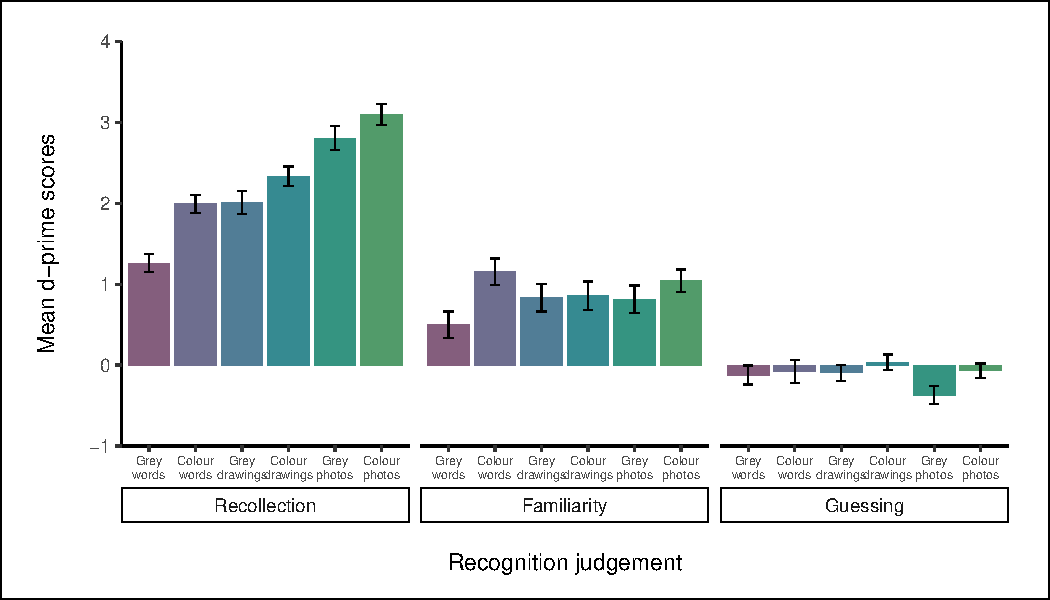
\includegraphics{R--Thesis_files/figure-latex/unnamed-chunk-91-1.pdf}
Figure 25: Mean d' scores by stimuli format and recognition judgement.

\newpage

For responses assigned \emph{Recollection}, there was a significant main
effect of stimuli format for the mean proportion of hits
{[}\emph{F}(3.10, 486.70) = 73.92, \emph{p} \textless{} .001,
\(\eta^2_p\) = .32{]}, mean proportion of FAs {[}\emph{F}(4.38, 687.03)
= 3.89, \emph{p} = .003, \(\eta^2_p\) = .02{]}, and mean \emph{d'}
scores {[}\emph{F}(4.40, 690.83) = 40.88, \emph{p} \textless{} .001,
\(\eta^2_p\) = .21{]}.

\textbf{Distinctiveness manipulation (regular words vs.~distinctive
words):} Across each of the variables, the distinctive word stimuli
indeed appeared to be more distinctive than the regular words. Planned
comparisons showed that distinctive words (\emph{M} = 0.48) produced
significantly more R hits than regular words (\emph{M} = 0.36),
\emph{t}(157) = 4.74, \emph{p} \textless{} .001, \emph{d} = 0.38, and
also significantly higher \emph{d'} scores (distinctive words \emph{M} =
1.99, regular words \emph{M} = 1.26, \emph{t}(157) = 5.25, \emph{p}
\textless{} .001, \emph{d} = 0.42. Conversely, regular words (\emph{M} =
0.1) produced a significantly higher proportion of FAs assigned R than
distinctive words (\emph{M} = 0.04), \emph{t}(157) = -2.65, \emph{p} =
.009, \emph{d} = -0.21.

\textbf{Elimination of the PSE (distinctive words vs.~greyscale
drawings):} Grey drawings (\emph{M} = 0.56) produced a significantly
higher number of hits assigned R compared to the distinctive words
(\emph{M} = 0.48), \emph{t}(157) = -3.64, \emph{p} \textless{} .001,
\emph{d} = -0.29.

On the other hand, the distinctive words (\emph{M} = 0.04) produced
significantly fewer FAs assigned R than grey drawings (\emph{M} = 0.11),
\emph{t}(157) = -2.41, \emph{p} = .017, \emph{d} = -0.19. This somewhat
extended to the colour drawings, where there was no difference between
the distinctive words (\emph{M} = 0.04) and colour drawings (\emph{M} =
0.06), \emph{t}(157) = 0.71, \emph{p} = .478, \emph{d} = 0.06.
Comparisons with grey photos, however, showed a return of the PSE, as
the distinctive words (\emph{M} = 0.04) produced a significantly higher
number of R FAs than grey photo (\emph{M} = 0.07), \emph{t}(157) =
-2.41, \emph{p} = .017, \emph{d} = -0.19.

For \emph{d'} scores, there was an elimination of the PSE; distinctive
words (\emph{M} = 1.99) and grey drawings (\emph{M} = 2.01) showed no
significant difference in mean \emph{d'} scores, \emph{t}(157) = -0.09,
\emph{p} = .932, \emph{d} \textless{} 0.01.

\textbf{Extension to colour drawings}: Elimination of the PSE for
\emph{d'} scores did not extend to colour drawings. Colour drawings
(\emph{M} = 2.34) showed significantly higher \emph{d'} scores than the
distinctive words (\emph{M} = 1.99), \emph{t}(157) = 2.30, \emph{p} =
.023, \emph{d} = 0.18.

\textbf{Extension to photos:} Grey photos (\emph{M} = 2.81) showed
significantly higher \emph{d'} scores than the distinctive words
(\emph{M} = 1.99), \emph{t}(157) = -4.95, \emph{p} \textless{} .001,
\emph{d} = -0.39.

Colour photos (\emph{M} = 3.1) showed significantly higher \emph{d'}
scores than the distinctive words (\emph{M} = 1.99), \emph{t}(157) =
8.26, \emph{p} \textless{} .001, \emph{d} = 0.66.

\newpage

For responses assigned \emph{Familiarity}, there was again a significant
main effect of stimuli format across all of the variables; the mean
proportion of hits {[}\emph{F}(3.09, 484.95) = 25.45, \emph{p}
\textless{} .001, \(\eta^2_p\) = .14{]}, mean proportion of FAs
{[}\emph{F}(4.54, 713.44) = 15.62, \emph{p} \textless{} .001,
\(\eta^2_p\) = .09{]}, and mean \emph{d'} scores {[}\emph{F}(4.52,
709.38) = 2.52, \emph{p} = .033, \(\eta^2_p\) = .02{]}.

\textbf{Distinctiveness manipulation (regular words vs.~distinctive
words):}

Regular words (\emph{M} = 0.48) produced significantly more F hits than
the distinctive words (\emph{M} = 0.41), \emph{t}(157) = -2.53, \emph{p}
= .012, \emph{d} = -0.20, and significantly more F FAs (regular words
\emph{M} = 0.38, distinctive words \emph{M} = 0.19, \emph{t}(157) =
-4.56, \emph{p} \textless{} .001, \emph{d} = -0.36. \emph{d'} scores,
however, were significantly higher for the distinctive words (\emph{M} =
1.15) compared to the regular words (\emph{M} = 0.5), \emph{t}(157) =
2.93, \emph{p} = .004, \emph{d} = 0.23.

\textbf{Elimination of the PSE (distinctive words vs.~greyscale
drawings):}

For the proportion of F hits, the PSE was eliminated, with no
significant difference between distinctive words (\emph{M} = 0.41) and
grey drawings (\emph{M} = 0.38), \emph{t}(157) = 0.84, \emph{p} = .403,
\emph{d} = 0.07. Likewise, there was no significant difference for the
number of FAs assigned F between distinctive words (\emph{M} = 0.19) and
grey drawings (\emph{M} = 0.23), \emph{t}(157) = -1.24, \emph{p} = .219,
\emph{d} = -0.10. For \emph{d'} scores, there was again an elimination
of the PSE; distinctive words (\emph{M} = 1.15) and grey drawings
(\emph{M} = 0.83) showed no significant difference in mean \emph{d'}
scores, \emph{t}(157) = 1.54, \emph{p} = .125, \emph{d} = 0.12.

\textbf{Extension to colour drawings}: Elimination of the PSE for
\emph{d'} scores also extended to colour drawings. Mean \emph{d'} scores
were not significantly different between distinctive words (\emph{M} =
1.15) and colour drawings (\emph{M} = 0.86), \emph{t}(157) = -1.33,
\emph{p} = .184, \emph{d} = -0.11.

\textbf{Extension to photos:} Elimination of the PSE for \emph{d'}
scores also extended to grey photos. Mean \emph{d'} scores were not
significantly different between distinctive words (\emph{M} = 1.15) and
grey photos (\emph{M} = 0.81), \emph{t}(157) = 1.58, \emph{p} = .116,
\emph{d} = 0.13.

Elimination of the PSE for \emph{d'} scores also extended to colour
photos. Mean \emph{d'} scores were not significantly different between
distinctive words (\emph{M} = 1.15) and colour photos (\emph{M} = 1.04),
\emph{t}(157) = -0.63, \emph{p} = .527, \emph{d} = -0.05.

\newpage

For responses assigned \emph{Guessing}, there was a significant main
effect of stimuli format for the mean proportion of hits
{[}\emph{F}(2.99, 468.71) = 24.58, \emph{p} \textless{} .001,
\(\eta^2_p\) = .14{]} and mean proportion of FAs {[}\emph{F}(4.69,
736.23) = 4.66, \emph{p} \textless{} .001, \(\eta^2_p\) = .03{]}.
However, the main effect of mean \emph{d'} scores did not reach
significance {[}\emph{F}(4.51, 708.09) = 1.57, \emph{p} = .172,
\(\eta^2_p\) \textless{} .01{]}; visual inspection of this data shows
that across the stimuli formats, \emph{d'} scores were generally
negative for \emph{Guessing} responses, an expected pattern that shows
poor discrimination and often more FAs than hits.

\textbf{Distinctiveness manipulation (regular words vs.~distinctive
words):} There was no difference in the number of hits assigned G
between regular words (\emph{M} = 0.13) and distinctive words (\emph{M}
= 0.1), \emph{t}(157) = -1.75, \emph{p} = .082, \emph{d} = -0.14, no
difference in the number of FAs assigned G between regular words
(\emph{M} = 0.19) and distinctive words (\emph{M} = 0.15), \emph{t}(157)
= -1.10, \emph{p} = .275, \emph{d} = -0.09, and no difference in mean
\emph{d'} scores between regular words (\emph{M} = -0.12) and
distinctive words (\emph{M} = -0.08), \emph{t}(157) = 0.23, \emph{p} =
.815, \emph{d} = 0.02.

\textbf{Elimination of the PSE (distinctive words vs.~greyscale
drawings):}

For the proportion of G hits, the distinctive words (\emph{M} = 0.1)
produced a significantly higher proportion compared to the grey drawings
(\emph{M} = 0.05), \emph{t}(157) = 3.28, \emph{p} = .001, \emph{d} =
0.26. There was no significant difference for the number of FAs assigned
G between distinctive words (\emph{M} = 0.15) and grey drawings
(\emph{M} = 0.1), \emph{t}(157) = 1.41, \emph{p} = .161, \emph{d} =
0.11, or mean \emph{d'} scores (distinctive words \emph{M} = -0.08, grey
drawings \emph{M} = -0.1, \emph{t}(157) = 0.10, \emph{p} = .920,
\emph{d} \textless{} 0.01.

\hypertarget{discussion-4}{%
\subsubsection{Discussion}\label{discussion-4}}

Ensor et al. (2019) demonstrated how picture superiority effects (PSEs)
could be eliminated by increasing the distinctiveness of word stimuli
(relative to shaded drawings) via manipulations to colour, font, size,
and capitalisation. The current experiment aimed to replicate such
findings in order to examine whether such effect would extend to the
\emph{photograph} superiority effect (PhSE). The first hypothesis
proposed that the distinctive word stimuli would produce a higher
proportion of correct hits, lower proportion of false alarms (FAs), and
higher overall \emph{d'} scores in comparison to regular word stimuli,
however, these predictions were not wholly supported by the data. While
the distinctive words showed a lower proportion of FAs and higher
\emph{d'} scores compared to regular words, the formats did not differ
in the proportion of obtained hits.

It is difficult to conclude the distinctive word stimuli were indeed
more distinctive than the regular words on the basis of these findings.
In both Ensor et al. (2019) experiments, the distinctive words produced
a significantly higher proportion of hits compared to the regular words.
This is in contrast to the results of the current study, whereby no
difference was found as a result of the distinctiveness manipulation.
Visual inspection of the data does not indicate the number of trials had
an impact on the number of hits; while Ensor et al. (2019) did observe a
reduction in the proportion of hits for both word formats when trial
numbers were increased, the current study (whose trial numbers were
between the two Ensor et al. (2019) experiments) still showed a lower
proportion of hits than both.

Visual inspection of the data shows that subjects generally made more
FAs in the Ensor et al. (2019) experiments compared to the current
study; this is especially apparent when comparisons are made toward the
experiment with more trials.

Visual inspection of the data shows that the \emph{d'} scores obtained
in the current experiment sit between the Ensor et al. (2019)
experiments - in line with reducing scores as the number of trials
increases.

pertained to the current manipulation, whereby the word items with
manipulations to colour, font, and capitalisation were expected to
produce enhanced recognition relative to regular word stimuli.

The current study has two primary aims: i) replicate the elimination of
the PSE demonstrated by Ensor et al. (2019); ii) examine whether the
PhSE is also attenuated / eliminated when comparing photograph items
with distinctive word stimuli. A secondary aim is to further
characterise the role of colour in the previously established
\emph{photo} superiority effect (PhSE).

It is not entirely clear why

The second hypothesis proposed standard picture superiority effects
(PSEs) would emerge - a finding that was abundantly clear when examining
the data, with \emph{all} pictures (greyscale drawings; colour drawings;
greyscale photographs; colour photographs) demonstrating superior
performance compared to regular words (manifesting as significantly
higher proportions of hits, lower proportions of FAs, and a higher mean
\emph{d'} scores). In a similar fashion, \emph{photo} superiority
effects (PhSEs) were also demonstrated when comparing performance for
photograph items against that of drawing items; this effect was evident
in both greyscale items (replicating the finding of \emph{Experiment 3})
and colour items (replicating the finding of \emph{Experiment 4}).

A limitation of the current study lies in its' inability to determine
how a number of factors separately contribute toward an overall level of
distinctiveness. Such a

Ensor et al. (2019) designed distinctive word stimuli that contained
manipulations to colour, font, size, and capitalisation, however, there
was little rationale for why these particular factors were selected.

Such comparisons are outside the scope of the current programme of
research, where innumerable combinations of such factors would need to
be compared

It could simply be assumed that each of these factors provide similar
contributions, and that they each play a role in the overall levels of
distinctiveness of a stimulus. However, across three experiments, the
current programme of research has consistently demonstrated that colour
information has no discernible impact on recognition performance - and
as such, does not contribute to making stimuli more distinctive.

\newpage

\#\#\#\#\#\#----------------------------------------

\newpage

\hypertarget{chapter-6}{%
\section{Chapter 6}\label{chapter-6}}

\hypertarget{background-4}{%
\subsection{Background}\label{background-4}}

DCT does not operate in absolutes. Both words and pictures have the
ability to generate dual codes: words (verbal by default, but image code
can be generated by conjuring a mental image of the items referent)
pictures (imagery by default, but verbal name can be internally
generated when identifying the item)

Explanations of the PSE boil down to \emph{likelihood}. It's much more
likely that pictures are also named (low effort process) than it is for
words to be imagined (effortful). Thus, the likelihood of pictures
generating dual codes is higher than that for words, aiding recognition
/ retrieval later on.

While results this far seem best explained by the physical
distinctiveness account, DCT cannot be discounted entirely.
Manipulations to stimuli distinctiveness might simply affect the
likelihood that 2nd codes are generated. Dual codes highly likely for
photographs, likely for drawings, less likely for words. Perhaps results
are best explained by a unified theory of the PSE. concreteness effect -
see Ensor et al. (2019), blue highlight on 2nd page.

\hypertarget{experiment-manipulating-word-labels}{%
\subsection{Experiment: Manipulating word
labels}\label{experiment-manipulating-word-labels}}

2 participants were removed due to a programming error, whereby pictures
without labels were not presented.

\newpage

\hypertarget{references}{%
\section{References}\label{references}}

\setlength{\parindent}{-0.2in}
\setlength{\leftskip}{0.2in}
\setlength{\parskip}{8pt}

\noindent

\hypertarget{refs}{}
\leavevmode\hypertarget{ref-adlington2009}{}%
Adlington, R. L., Laws, K. R., \& Gale, T. M. (2009). The Hatfield Image
Test (HIT): A new picture test and norms for experimental and clinical
use. \emph{Journal of Clinical and Experimental Neuropsychology},
\emph{31}(6), 731--753. \url{https://doi.org/10.1080/13803390802488103}

\leavevmode\hypertarget{ref-algarabel2009}{}%
Algarabel, S., Escudero, J., Mazón, J. F., Pitarque, A., Fuentes, M.,
Peset, V., \& Lacruz, L. (2009). Familiarity-based recognition in the
young, healthy elderly, mild cognitive impaired and Alzheimer's
patients73. \emph{Neuropsychologia}, \emph{47}(10), 2056--2064.
\url{https://doi.org/10.1016/j.neuropsychologia.2009.03.016}

\leavevmode\hypertarget{ref-algarabel2012}{}%
Algarabel, S., Fuentes, M., Escudero, J., Pitarque, A., Peset, V.,
Mazón, J.-F., \& Meléndez, J.-C. (2012). Recognition memory deficits in
mild cognitive impairment. \emph{Aging, Neuropsychology, and Cognition},
\emph{19}(5), 608--619.
\url{https://doi.org/10.1080/13825585.2011.640657}

\leavevmode\hypertarget{ref-ally2012}{}%
Ally, B. A. (2012). Using Pictures and Words To Understand Recognition
Memory Deterioration in Amnestic Mild Cognitive Impairment and
Alzheimer's Disease: A Review. \emph{Current Neurology and Neuroscience
Reports}, \emph{12}(6), 687--694.
\url{https://doi.org/10.1007/s11910-012-0310-7}

\leavevmode\hypertarget{ref-ally2007}{}%
Ally, B. A., \& Budson, A. E. (2007). The worth of pictures: Using high
density event-related potentials to understand the memorial power of
pictures and the dynamics of recognition memory. \emph{NeuroImage},
\emph{35}(1), 378--395.
\url{https://doi.org/10.1016/j.neuroimage.2006.11.023}

\leavevmode\hypertarget{ref-ally2009}{}%
Ally, B. A., Gold, C. A., \& Budson, A. E. (2009a). The picture
superiority effect in patients with Alzheimer's disease and mild
cognitive impairment. \emph{Neuropsychologia}, \emph{47}(2), 595--598.
\url{https://doi.org/10.1016/j.neuropsychologia.2008.10.010}

\leavevmode\hypertarget{ref-ally2009a}{}%
Ally, B. A., McKeever, J. D., Waring, J. D., \& Budson, A. E. (2009b).
Preserved frontal memorial processing for pictures in patients with mild
cognitive impairment. \emph{Neuropsychologia}, \emph{47}(10),
2044--2055. \url{https://doi.org/10.1016/j.neuropsychologia.2009.03.015}

\leavevmode\hypertarget{ref-ally2008}{}%
Ally, B. A., Waring, J. D., Beth, E. H., McKeever, J. D., Milberg, W.
P., \& Budson, A. E. (2008). Aging memory for pictures: Using
high-density event-related potentials to understand the effect of aging
on the picture superiority effect. \emph{Neuropsychologia},
\emph{46}(2), 679--689.
\url{https://doi.org/10.1016/j.neuropsychologia.2007.09.011}

\leavevmode\hypertarget{ref-anderson2008}{}%
Anderson, N. D., Ebert, P. L., Jennings, J. M., Grady, C. L., Cabeza,
R., \& Graham, S. J. (2008). Recollection- and familiarity-based memory
in healthy aging and amnestic mild cognitive impairment.
\emph{Neuropsychology}, \emph{22}(2), 177--187.
\url{https://doi.org/10.1037/0894-4105.22.2.177}

\leavevmode\hypertarget{ref-barba1997}{}%
Barba, G. D. (1997). Recognition Memory and Recollective Experience in
Alzheimer's Disease. \emph{Memory}, \emph{5}(6), 657--672.
\url{https://doi.org/10.1080/741941546}

\leavevmode\hypertarget{ref-bastin2004}{}%
Bastin, C., Van der Linden, M., Michel, A.-P., \& Friedman, W. J.
(2004). The effects of aging on location-based and distance-based
processes in memory for time. \emph{Acta Psychologica}, \emph{116}(2),
145--171. \url{https://doi.org/10.1016/j.actpsy.2003.12.014}

\leavevmode\hypertarget{ref-belleville2011}{}%
Belleville, S., Ménard, M.-C., \& Lepage, É. (2011). Impact of novelty
and type of material on recognition in healthy older adults and persons
with mild cognitive impairment. \emph{Neuropsychologia},
\emph{49}(2011), 2856--2865.

\leavevmode\hypertarget{ref-bermudez-margaretto2018}{}%
Bermúdez-Margaretto, B., Beltrán, D., Cuetos, F., \& Domínguez, A.
(2018). Brain Signatures of New (Pseudo-) Words: Visual Repetition in
Associative and Non-associative Contexts. \emph{Frontiers in Human
Neuroscience}, \emph{12}, 354.
\url{https://doi.org/10.3389/fnhum.2018.00354}

\leavevmode\hypertarget{ref-biederman1987}{}%
Biederman, I. (1987). \emph{Recognition-by-Components: A Theory of Human
Image Understanding}. 33.

\leavevmode\hypertarget{ref-bowen2019}{}%
Bowen, H. J., Fields, E. C., \& Kensinger, E. A. (2019). Prior Emotional
Context Modulates Early Event-Related Potentials to Neutral Retrieval
Cues. \emph{Journal of Cognitive Neuroscience}, \emph{31}(11),
1755--1767. \url{https://doi.org/10.1162/jocn_a_01451}

\leavevmode\hypertarget{ref-brown2011}{}%
Brown, A. A., \& Bodner, G. E. (2011). Re-examining dissociations
between remembering and knowing: Binary judgments vs. Independent
ratings. \emph{Journal of Memory and Language}, \emph{65}(2), 98--108.
\url{https://doi.org/10.1016/j.jml.2011.04.003}

\leavevmode\hypertarget{ref-cui2016}{}%
Cui, L., Shi, G., He, F., Zhang, Q., Oei, T. P. S., \& Guo, C. (2016).
Electrophysiological Correlates of Emotional Source Memory in
High-Trait-Anxiety Individuals. \emph{Frontiers in Psychology},
\emph{7}. \url{https://doi.org/10.3389/fpsyg.2016.01039}

\leavevmode\hypertarget{ref-curran2011}{}%
Curran, T., \& Doyle, J. (2011). Picture Superiority Doubly Dissociates
the ERP Correlates of Recollection and Familiarity. \emph{Journal of
Cognitive Neuroscience}, \emph{23}(5), 1247--1262.
\url{https://doi.org/10.1162/jocn.2010.21464}

\leavevmode\hypertarget{ref-deason2015}{}%
Deason, R. G., Hussey, E. P., Flannery, S., \& Ally, B. A. (2015).
Preserved conceptual implicit memory for pictures in patients with
Alzheimer's disease. \emph{Brain and Cognition}, \emph{99}, 112--117.
\url{https://doi.org/10.1016/j.bandc.2015.07.008}

\leavevmode\hypertarget{ref-dewhurst1994}{}%
Dewhurst, S. A., \& Conway, M. A. (1994). \emph{Pictures, Images, and
Recollective Experience}. 11.

\leavevmode\hypertarget{ref-dobbins1998}{}%
Dobbins, I. G., KroU, N. E. A., \& Liu, Q. (1998). Confidence-Accuracy
Inversions in Scene Recognition: A Remember-Know Analysis. \emph{Journal
of Experimental Psychology: Learning, Memory, and Cognition},
\emph{24}(5), 1306--1315.

\leavevmode\hypertarget{ref-donaldson1996}{}%
Donaldson, W., Mackenzie, T. M., \& Underhill, C. F. (1996). A
comparison of recollective memory and source monitoring.
\emph{Psychonomic Bulletin \& Review}, \emph{3}(4), 486--490.
\url{https://doi.org/10.3758/BF03214551}

\leavevmode\hypertarget{ref-dunn2008}{}%
Dunn, J. C. (2008). The Dimensionality of the RememberKnow Task: A
State-Trace Analysis. \emph{Psychological Review}, \emph{115}(2),
426--446.

\leavevmode\hypertarget{ref-eldridge2002}{}%
Eldridge, L. L., Sarfatti, S., \& Knowlton, B. J. (2002). The effect of
testing procedure on remember-know judgments. \emph{Psychonomic Bulletin
\& Review}, \emph{9}(1), 139--145.
\url{https://doi.org/10.3758/BF03196270}

\leavevmode\hypertarget{ref-embree2012}{}%
Embree, L. M., Budson, A. E., \& Ally, B. A. (2012). Memorial
familiarity remains intact for pictures but not for words in patients
with amnestic mild cognitive impairment. \emph{Neuropsychologia},
\emph{50}(9), 2333--2340.
\url{https://doi.org/10.1016/j.neuropsychologia.2012.06.001}

\leavevmode\hypertarget{ref-ensor2019b}{}%
Ensor, T. M., Surprenant, A. M., \& Neath, I. (2019). Increasing word
distinctiveness eliminates the picture superiority effect in
recognition: Evidence for the physical-distinctiveness account.
\emph{Memory \& Cognition}, \emph{47}(1), 182--193.
\url{https://doi.org/10.3758/s13421-018-0858-9}

\leavevmode\hypertarget{ref-faul2009}{}%
Faul, F., Erdfelder, E., Buchner, A., \& Lang, A.-G. (2009). Statistical
power analyses using G*Power 3.1: Tests for correlation and regression
analyses. \emph{Behavior Research Methods}, \emph{41}(4), 1149--1160.
\url{https://doi.org/10.3758/BRM.41.4.1149}

\leavevmode\hypertarget{ref-gardiner2000}{}%
Gardiner, J. M. (2000). On the objectivity of subjective experiences of
autonoetic and noetic consciousness. In E. Tulving (Ed.), \emph{Memory,
consciousness, and the brain: The Tallinn Conference} (pp. 159--172).
Psychology Press.

\leavevmode\hypertarget{ref-gardiner1996}{}%
Gardiner, J. M., Java, R. I., \& Richardson-Klavehn, A. (1996). How
level of processing really influences awareness in recognition memory.
\emph{Canadian Journal of Experimental Psychology/Revue Canadienne de
Psychologie Expérimentale}, \emph{50}(1), 114--122.
\url{https://doi.org/10.1037/1196-1961.50.1.114}

\leavevmode\hypertarget{ref-gardiner1998}{}%
Gardiner, J. M., \& Ramponi, C. (1998). Experiences of Remembering,
Knowing, and Guessing. \emph{CONSCIOUSNESS AND COGNITION}, \emph{7},
1--26.

\leavevmode\hypertarget{ref-gardiner2002a}{}%
Gardiner, J. M., Ramponi, C., \& Richardson-Klavehn, A. (2002).
Recognition memory and decision processes: A meta-analysis of remember,
know, and guess responses. \emph{Memory}, \emph{10}(2), 83--98.

\leavevmode\hypertarget{ref-geraci2009a}{}%
Geraci, L., McCabe, D. P., \& Guillory, J. J. (2009). On interpreting
the relationship between rememberKnow judgments and confidence: The role
of instructions. \emph{Consciousness and Cognition}, \emph{18}(3),
701--709. \url{https://doi.org/10.1016/j.concog.2009.04.010}

\leavevmode\hypertarget{ref-haber1982}{}%
Haber, R. N., \& Myers, B. L. (1982). Memory for Pictograms, Pictures,
and Words Separately and All Mixed up. \emph{Perception}, \emph{11}(1),
57--64. \url{https://doi.org/10.1068/p110057}

\leavevmode\hypertarget{ref-harlow2010}{}%
Harlow, I. M., MacKenzie, G., \& Donaldson, D. I. (2010). Familiarity
for associations? A test of the domain dichotomy theory. \emph{Journal
of Experimental Psychology: Learning, Memory, and Cognition},
\emph{36}(6), 1381--1388. \url{https://doi.org/10.1037/a0020610}

\leavevmode\hypertarget{ref-herzmann2018}{}%
Herzmann, G., Minor, G., \& Curran, T. (2018). Neural evidence for the
contribution of holistic processing but not attention allocation to the
other-race effect on face memory. \emph{Cognitive, Affective, \&
Behavioral Neuroscience}, \emph{18}(5), 1015--1033.
\url{https://doi.org/10.3758/s13415-018-0619-z}

\leavevmode\hypertarget{ref-higham2004}{}%
Higham, P. A., \& Vokey, J. R. (2004). Illusory Recollection and
DualProcess Models of Recognition Memory. \emph{The Quarterly Journal of
Experimental Psychology Section A}, \emph{57}(4), 714--744.
\url{https://doi.org/10.1080/02724980343000468}

\leavevmode\hypertarget{ref-hockley2008}{}%
Hockley, W. E. (2008). The picture superiority effect in associative
recognition. \emph{Memory \& Cognition}, \emph{36}(7), 1351--1359.
\url{https://doi.org/10.3758/MC.36.7.1351}

\leavevmode\hypertarget{ref-hudon2009}{}%
Hudon, C., Belleville, S., \& Gauthier, S. (2009). The assessment of
recognition memory using the Remember/Know procedure in amnestic mild
cognitive impairment and probable Alzheimer's disease. \emph{Brain and
Cognition}, 9.

\leavevmode\hypertarget{ref-ingram2012}{}%
Ingram, K. M., Mickes, L., \& Wixted, J. T. (2012). Recollection can be
weak and familiarity can be strong. \emph{Journal of Experimental
Psychology: Learning, Memory, and Cognition}, \emph{38}(2), 325--339.
\url{https://doi.org/10.1037/a0025483}

\leavevmode\hypertarget{ref-jacoby1991}{}%
Jacoby, L. L. (1991). A process dissociation framework: Separating
automatic from intentional uses of memory. \emph{Journal of Memory and
Language}, \emph{30}(5), 513--541.
\url{https://doi.org/10.1016/0749-596X(91)90025-F}

\leavevmode\hypertarget{ref-jacoby1997}{}%
Jacoby, L. L., Yonelinas, A. P., \& Jennings, J. M. (1997). The relation
between conscious and unconscious (automatic) influences: A declaration
of independence. In J. D. Cohen \& J. W. Schooler (Eds.),
\emph{Scientific approaches to consciousness} (pp. 13--47). Mahwah, NJ:
Erlbaum.

\leavevmode\hypertarget{ref-rstatix}{}%
Kassambara, A. (2020). \emph{Rstatix: Pipe-friendly framework for basic
statistical tests} {[}Manual{]}.

\leavevmode\hypertarget{ref-koen2014}{}%
Koen, J. D., \& Yonelinas, A. P. (2014). \emph{The Effects of Healthy
Aging, Amnestic Mild Cognitive Impairment, and Alzheimer's Disease on
Recollection and Familiarity: A Meta-Analytic Review}. 41.

\leavevmode\hypertarget{ref-kurilla2008}{}%
Kurilla, B. P., \& Westerman, D. L. (2008). Processing fluency affects
subjective claims of recollection. \emph{Memory \& Cognition},
\emph{36}(1), 82--92. \url{https://doi.org/10.3758/MC.36.1.82}

\leavevmode\hypertarget{ref-larsson2006}{}%
Larsson, M., Öberg, C., \& Bäckman, L. (2006). Recollective experience
in odor recognition: Influences of adult age and familiarity.
\emph{Psychological Research Psychologische Forschung}, \emph{70}(1),
68--75. \url{https://doi.org/10.1007/s00426-004-0190-9}

\leavevmode\hypertarget{ref-lombardi2016}{}%
Lombardi, M. G., Perri, R., Fadda, L., Caltagirone, C., \& Carlesimo, G.
A. (2016). Forgetting of the recollection and familiarity components of
recognition in patients with amnestic mild cognitive impairment.
\emph{Journal of Neuropsychology}, \emph{12}(2), 231--247.
\url{https://doi.org/10.1111/jnp.12114}

\leavevmode\hypertarget{ref-martins2006}{}%
Martins, C. A. R., \& Lloyd-Jones, T. J. (2006). Preserved Conceptual
Priming in Alzheimer's Disease. \emph{Cortex}, \emph{42}(7), 995--1004.
\url{https://doi.org/10.1016/S0010-9452(08)70205-3}

\leavevmode\hypertarget{ref-mayes2007}{}%
Mayes, A., Montaldi, D., \& Migo, E. (2007). Associative memory and the
medial temporal lobes. \emph{Trends in Cognitive Sciences},
\emph{11}(3), 126--135. \url{https://doi.org/10.1016/j.tics.2006.12.003}

\leavevmode\hypertarget{ref-mcbride2002}{}%
McBride, D. M., \& Anne Dosher, B. (2002). A comparison of conscious and
automatic memory processes for picture and word stimuli: A process
dissociation analysis. \emph{Consciousness and Cognition}, \emph{11}(3),
423--460. \url{https://doi.org/10.1016/S1053-8100(02)00007-7}

\leavevmode\hypertarget{ref-meade2019}{}%
Meade, M. E., Ahmad, M., \& Fernandes, M. A. (2019). Drawing pictures at
encoding enhances memory in healthy older adults and in individuals with
probable dementia. \emph{Aging, Neuropsychology, and Cognition},
\emph{27}(6), 880--901.
\url{https://doi.org/10.1080/13825585.2019.1700899}

\leavevmode\hypertarget{ref-migo2012}{}%
Migo, E. M., Mayes, A. R., \& Montaldi, D. (2012). Measuring
recollection and familiarity: Improving the remember/know procedure.
\emph{Consciousness and Cognition}, \emph{21}(3), 1435--1455.
\url{https://doi.org/10.1016/j.concog.2012.04.014}

\leavevmode\hypertarget{ref-mintzer1999}{}%
Mintzer, M. Z., \& Snodgrass, J. G. (1999). The Picture Superiority
Effect: Support for the Distinctiveness Model. \emph{The American
Journal of Psychology}, \emph{112}(1), 113.
\url{https://doi.org/10.2307/1423627}

\leavevmode\hypertarget{ref-moreno-martinez2012}{}%
Moreno-Martínez, F. J., \& Montoro, P. R. (2012). An Ecological
Alternative to Snodgrass \& Vanderwart: 360 High Quality Colour Images
with Norms for Seven Psycholinguistic Variables. \emph{PLoS ONE},
\emph{7}(5), e37527. \url{https://doi.org/10.1371/journal.pone.0037527}

\leavevmode\hypertarget{ref-oconnor2010}{}%
O'Connor, M. K., \& Ally, B. A. (2010). Using stimulus form change to
understand memorial familiarity for pictures and words in patients with
mild cognitive impairment and Alzheimer's disease.
\emph{Neuropsychologia}, \emph{48}(7), 2068--2074.
\url{https://doi.org/10.1016/j.neuropsychologia.2010.03.027}

\leavevmode\hypertarget{ref-paivio1971}{}%
Paivio, A. (1971). \emph{Imagery and verbal processes.} New York: Holt,
Rinehart and Winston.

\leavevmode\hypertarget{ref-paivio1972}{}%
Paivio, A. (1972). Symbolic and sensory modalities of memory. In M. E.
Meyer (Ed.), \emph{The third Western symposium on learning: Cognitive
Learning.} Western Washington State College.

\leavevmode\hypertarget{ref-paivio1991}{}%
Paivio, A. (1991). Dual coding theory: Retrospect and current status.
\emph{Canadian Journal of Psychology/Revue Canadienne de Psychologie},
\emph{45}(3), 255--287. \url{https://doi.org/10.1037/h0084295}

\leavevmode\hypertarget{ref-paivio2007}{}%
Paivio, A. (2007). \emph{Mind and its evolution: A dual coding
theoretical approach.} Lawrence Erlbaum Associates Publishers.

\leavevmode\hypertarget{ref-paivio1968}{}%
Paivio, A., Rogers, T. B., \& Smythe, P. C. (1968). Why are pictures
easier to recall than words? \emph{Psychonomic Science}, \emph{11}(4),
137--138. \url{https://doi.org/10.3758/BF03331011}

\leavevmode\hypertarget{ref-peeck1977}{}%
Peeck, J., Van Dam, G., \& Uhlenbeck, R. W. F. (1977). Incidental Cues
and Picture/Word Differences in Recall. \emph{Perceptual and Motor
Skills}, \emph{45}(3\_suppl), 1211--1215.
\url{https://doi.org/10.2466/pms.1977.45.3f.1211}

\leavevmode\hypertarget{ref-peirce2019}{}%
Peirce, J., Gray, J. R., Simpson, S., MacAskill, M., Höchenberger, R.,
Sogo, H., \ldots{} Lindeløv, J. K. (2019). PsychoPy2: Experiments in
behavior made easy. \emph{Behavior Research Methods}, \emph{51}(1),
195--203. \url{https://doi.org/10.3758/s13428-018-01193-y}

\leavevmode\hypertarget{ref-pitarque2016}{}%
Pitarque, A. (2016). \emph{The effects of healthy aging, amnestic mild
cognitive impairment, and Alzheimer's disease on recollection,
familiarity and false recognition, estimated by an associative
process-dissociation recognition procedure}. 7.

\leavevmode\hypertarget{ref-rajaram1993}{}%
Rajaram, S. (1993). Remembering and knowing: Two means of access to the
personal past. \emph{Memory \& Cognition}, \emph{21}(1), 89--102.
\url{https://doi.org/10.3758/BF03211168}

\leavevmode\hypertarget{ref-rajaram1996a}{}%
Rajaram, S. (1996a). Perceptual Effects on Remembering: Recollective
Processes in Picture Recognition Memory. \emph{Journal of Experimental
Psychology: Learning, Memory, and Cognition}, \emph{22}(2), 365--377.

\leavevmode\hypertarget{ref-rajaram1996}{}%
Rajaram, S. (1996b). \emph{Perceptual Effects on Remembering:
Recollective Processes in Picture Recognition Memory}. 13.

\leavevmode\hypertarget{ref-rcoreteam2020}{}%
R Core Team. (2020). \emph{R: A language and environment for statistical
computing} {[}Manual{]}. Vienna, Austria: R Foundation for Statistical
Computing.

\leavevmode\hypertarget{ref-rollins2018}{}%
Rollins, L., \& Riggins, T. (2018). Age-related differences in
subjective recollection: ERP studies of encoding and retrieval.
\emph{Developmental Science}, \emph{21}(3), e12583.
\url{https://doi.org/10.1111/desc.12583}

\leavevmode\hypertarget{ref-rossion2004}{}%
Rossion, B., \& Pourtois, G. (2004). Revisiting Snodgrass and
Vanderwart's Object Pictorial Set: The Role of Surface Detail in
Basic-Level Object Recognition. \emph{Perception}, \emph{33}(2),
217--236. \url{https://doi.org/10.1068/p5117}

\leavevmode\hypertarget{ref-rubin2015}{}%
Rubin, D. C., \& Umanath, S. (2015). Event memory: A theory of memory
for laboratory, autobiographical, and fictional events.
\emph{Psychological Review}, \emph{122}(1), 1--23.
\url{https://doi.org/10.1037/a0037907}

\leavevmode\hypertarget{ref-sanfeliu1996}{}%
Sanfeliu, M. C., \& Fernandez, A. (1996). A set of 254
Snodgrass-Vanderwart pictures standardized for Spanish: Norms for name
agreement, image agreement, familiarity, and visual complexity.
\emph{Behavior Research Methods, Instruments, \& Computers},
\emph{28}(4), 537--555. \url{https://doi.org/10.3758/BF03200541}

\leavevmode\hypertarget{ref-scalici2017}{}%
Scalici, F., Caltagirone, C., \& Carlesimo, G. A. (2017). The
contribution of different prefrontal cortex regions to recollection and
familiarity: A review of fMRI data. \emph{Neuroscience \& Biobehavioral
Reviews}, \emph{83}, 240--251.
\url{https://doi.org/10.1016/j.neubiorev.2017.10.017}

\leavevmode\hypertarget{ref-schmitter-edgecombe2009}{}%
Schmitter-Edgecombe, M., Woo, E., \& Greeley, D. R. (2009).
Characterizing multiple memory deficits and their relation to everyday
functioning in individuals with mild cognitive impairment.
\emph{Neuropsychology}, \emph{23}(2), 168--177.
\url{https://doi.org/10.1037/a0014186}

\leavevmode\hypertarget{ref-schoemaker2014}{}%
Schoemaker, D., Gauthier, S., \& Pruessner, J. C. (2014). Recollection
and Familiarity in Aging Individuals with Mild Cognitive Impairment and
Alzheimer's Disease: A Literature Review. \emph{Neuropsychol Rev}, 19.

\leavevmode\hypertarget{ref-serra2010}{}%
Serra, L., Bozzali, M., Cercignani, M., Perri, R., Fadda, L.,
Caltagirone, C., \& Carlesimo, G. A. (2010). Recollection and
familiarity in amnesic mild cognitive impairment.
\emph{Neuropsychology}, \emph{24}(3), 316--326.
\url{https://doi.org/10.1037/a0017654}

\leavevmode\hypertarget{ref-shepard1967}{}%
Shepard, R. N. (1967). Recognition memory for words, sentences, and
pictures. \emph{Journal of Verbal Learning and Verbal Behavior},
\emph{6}(1), 156--163.
\url{https://doi.org/10.1016/S0022-5371(67)80067-7}

\leavevmode\hypertarget{ref-afex}{}%
Singmann, H., Bolker, B., Westfall, J., Aust, F., \& Ben-Shachar, M. S.
(2020). \emph{Afex: Analysis of factorial experiments} {[}Manual{]}.

\leavevmode\hypertarget{ref-snodgrass1980}{}%
Snodgrass, J. G., \& Vanderwart, M. (1980). A Standardized Set of 260
Pictures: Norms for Name Agreement, Image Agreement, Familiarity, and
Visual Complexity. \emph{Journal of Experimental Psychology: Human
Learning and Memory}, \emph{6}(2), 174--215.

\leavevmode\hypertarget{ref-squire2007}{}%
Squire, L. R., Wixted, J. T., \& Clark, R. E. (2007). Recognition memory
and the medial temporal lobe: A new perspective. \emph{Nature Reviews.
Neuroscience}, \emph{8}(11), 872--883.
\url{https://doi.org/10.1038/nrn2154}

\leavevmode\hypertarget{ref-stenberg2006}{}%
Stenberg, G. (2006). Conceptual and perceptual factors in the picture
superiority effect. \emph{European Journal of Cognitive Psychology},
\emph{18}(6), 813--847. \url{https://doi.org/10.1080/09541440500412361}

\leavevmode\hypertarget{ref-suzuki1997}{}%
Suzuki, K., \& Takahashi, R. (1997). Effectiveness of color in picture
recognition memory. \emph{Japanese Psychological Research},
\emph{39}(1), 25--32. \url{https://doi.org/10.1111/1468-5884.00033}

\leavevmode\hypertarget{ref-szekely2003}{}%
Székely, A., D'Amico, S., Devescovi, A., Federmeier, K., Herron, D.,
Iyer, G., \ldots{} Bates, E. (2003). Timed picture naming: Extended
norms and validation against previous studies. \emph{Behavior Research
Methods, Instruments, \& Computers}, \emph{35}(4), 621--633.
\url{https://doi.org/10.3758/BF03195542}

\leavevmode\hypertarget{ref-tanaka2001}{}%
Tanaka, J., Weiskopf, D., \& Williams, P. (2001). The role of color in
high-level vision. \emph{TRENDS in Cognitive Sciences}, \emph{5}(5),
211--215.

\leavevmode\hypertarget{ref-tarr1998}{}%
Tarr, M. J., \& Bülthoff, H. H. (1998). Image-based object recognition
in man, monkey and machine. \emph{Cognition}, \emph{67}(1-20).

\leavevmode\hypertarget{ref-tousignant2012}{}%
Tousignant, C., \& Bodner, G. E. (2012). Test context affects
recollection and familiarity ratings: Implications for measuring
recognition experiences. \emph{Consciousness and Cognition},
\emph{21}(2), 994--1000.
\url{https://doi.org/10.1016/j.concog.2012.01.009}

\leavevmode\hypertarget{ref-tousignant2015}{}%
Tousignant, C., Bodner, G. E., \& Arnold, M. M. (2015). Effects of
context on recollection and familiarity experiences are task dependent.
\emph{Consciousness and Cognition}, \emph{33}, 78--89.
\url{https://doi.org/10.1016/j.concog.2014.11.011}

\leavevmode\hypertarget{ref-troyer2012}{}%
Troyer, A. K., Murphy, K. J., Anderson, N. D., Craik, F. I. M.,
Moscovitch, M., Maione, A., \& Gao, F. (2012). Associative recognition
in mild cognitive impairment: Relationship to hippocampal volume and
apolipoprotein E. \emph{Neuropsychologia}, \emph{50}(14), 3721--3728.
\url{https://doi.org/10.1016/j.neuropsychologia.2012.10.018}

\leavevmode\hypertarget{ref-troyer2016}{}%
Troyer, A. K., Vandermorris, S., \& Murphy, K. J. (2016).
Intraindividual variability in performance on associative memory tasks
is elevated in amnestic mild cognitive impairment.
\emph{Neuropsychologia}, \emph{90}, 110--116.
\url{https://doi.org/10.1016/j.neuropsychologia.2016.06.011}

\leavevmode\hypertarget{ref-tsaparina2011}{}%
Tsaparina, D., Bonin, P., \& Méot, A. (2011). Russian norms for name
agreement, image agreement for the colorized version of the Snodgrass
and Vanderwart pictures and age of acquisition, conceptual familiarity,
and imageability scores for modal object names. \emph{Behavior Research
Methods}, \emph{43}(4), 1085--1099.
\url{https://doi.org/10.3758/s13428-011-0121-9}

\leavevmode\hypertarget{ref-tulving1985}{}%
Tulving, E. (1985). Memory and consciousness. \emph{Canadian
Psychology/Psychologie Canadienne}, \emph{26}(1), 1--12.
\url{https://doi.org/10.1037/h0080017}

\leavevmode\hypertarget{ref-tunney2007}{}%
Tunney, R. J., \& Fernie, G. (2007). Repetition priming affects guessing
not familiarity. \emph{Behavioral and Brain Functions}, \emph{3}(1), 40.
\url{https://doi.org/10.1186/1744-9081-3-40}

\leavevmode\hypertarget{ref-umanath2020}{}%
Umanath, S., \& Coane, J. H. (2020). Face Validity of Remembering and
Knowing: Empirical Consensus and Disagreement Between Participants and
Researchers. \emph{Perspectives on Psychological Science}, \emph{15}(6),
1400--1422. \url{https://doi.org/10.1177/1745691620917672}

\leavevmode\hypertarget{ref-vandermeulen2012}{}%
van der Meulen, M., Lederrey, C., Rieger, S. W., van Assche, M.,
Schwartz, S., Vuilleumier, P., \& Assal, F. (2012). Associative and
Semantic Memory Deficits in Amnestic Mild Cognitive Impairment as
Revealed by Functional Magnetic Resonance Imaging: \emph{Cognitive and
Behavioral Neurology}, \emph{25}(4), 195--215.
\url{https://doi.org/10.1097/WNN.0b013e31827de67f}

\leavevmode\hypertarget{ref-viggiano2004}{}%
Viggiano, M. P., Vannucci, M., \& Righi, S. (2004). A New Standardized
Set of Ecological Pictures for Experimental and Clinical Research on
Visual Object Processing. \emph{Cortex}, \emph{40}(3), 491--509.
\url{https://doi.org/10.1016/S0010-9452(08)70142-4}

\leavevmode\hypertarget{ref-wagner1997}{}%
Wagner, A. D., Gabrieli, J. D. E., \& Verfaellie, M. (1997).
\emph{Dissociations Between Familiarity Processes in Explicit
Recognition and Implicit Perceptual Memory}. 19.

\leavevmode\hypertarget{ref-wammes2016}{}%
Wammes, J. D., Meade, M. E., \& Fernandes, M. A. (2016). The drawing
effect: Evidence for reliable and robust memory benefits in free recall.
\emph{Quarterly Journal of Experimental Psychology}, \emph{69}(9),
1752--1776. \url{https://doi.org/10.1080/17470218.2015.1094494}

\leavevmode\hypertarget{ref-wang2013a}{}%
Wang, P., Li, J., Li, H., Li, B., Yang Jiang, Bao, F., \& Zhang, S.
(2013). Is emotional memory enhancement preserved in amnestic mild
cognitive impairment? Evidence from separating recollection and
familiarity. \emph{Neuropsychology}, \emph{27}(6), 691--701.
\url{https://doi.org/10.1037/a0033973}

\leavevmode\hypertarget{ref-wang2013}{}%
Wang, Li, H., Liang, Y., Zhang, J., Li, X., Shu, N., \ldots{} Zhang, Z.
(2013). Amnestic Mild Cognitive Impairment: Topological Reorganization
of the Default-Mode Network. \emph{Radiology}, \emph{268}(2), 501--514.
\url{https://doi.org/10.1148/radiol.13121573}

\leavevmode\hypertarget{ref-weldon1989}{}%
Weldon, M. S., Iii, H. L. R., \& Challis, B. H. (1989). \emph{The
properties of retrieval cues constrain the picture superiority effect}.
11.

\leavevmode\hypertarget{ref-weldon1987}{}%
Weldon, M. S., \& Roediger, H. L. (1987). \emph{Altering retrieval
demands reverses the picture superiority effect}. 12.

\leavevmode\hypertarget{ref-westerberg2006}{}%
Westerberg, C. E., Paller, K. A., Weintraub, S., Mesulam, M.-M.,
Holdstock, J. S., Mayes, A. R., \& Reber, P. J. (2006). When memory does
not fail: Familiarity-based recognition in mild cognitive impairment and
Alzheimer's disease. \emph{Neuropsychology}, \emph{20}(2), 193--205.
\url{https://doi.org/10.1037/0894-4105.20.2.193}

\leavevmode\hypertarget{ref-westerberg2013}{}%
Westerberg, C., Mayes, A., Florczak, S. M., Chen, Y., Creery, J.,
Parrish, T., \ldots{} Paller, K. A. (2013). Distinct medial temporal
contributions to different forms of recognition in amnestic mild
cognitive impairment and Alzheimer's disease. \emph{Neuropsychologia},
\emph{51}(12), 2450--2461.
\url{https://doi.org/10.1016/j.neuropsychologia.2013.06.025}

\leavevmode\hypertarget{ref-whitehouse2006}{}%
Whitehouse, A. J. O., Maybery, M. T., \& Durkin, K. (2006). The
development of the picture-superiority effect. \emph{British Journal of
Developmental Psychology}, \emph{24}(4), 767--773.
\url{https://doi.org/10.1348/026151005X74153}

\leavevmode\hypertarget{ref-williams2019}{}%
Williams, H. L. (2019). \emph{Different definitions of the
nonrecollection-based response option(s) change how people use the
``remember'' response in the remember/know paradigm}. 16.

\leavevmode\hypertarget{ref-williams2014}{}%
Williams, H. L., \& Moulin, C. J. A. (2014). Know versus Familiar:
Differentiating states of awareness in others' subjective reports of
recognition. \emph{Memory}, \emph{23}(7), 981--990.
\url{https://doi.org/10.1080/09658211.2014.945460}

\leavevmode\hypertarget{ref-doi:https:ux2fux2fdoi.orgux2f10.1002ux2f9781118445112.stat06743}{}%
Wixted, J. T. (2014). Signal detection theory. In \emph{Wiley StatsRef:
Statistics reference online}. American Cancer Society.
\url{https://doi.org/10.1002/9781118445112.stat06743}

\leavevmode\hypertarget{ref-wolk2011}{}%
Wolk, D. A., Dunfee, K. L., Dickerson, B. C., Aizenstein, H. J., \&
DeKosky, S. T. (2011). A medial temporal lobe division of labor:
Insights from memory in aging and early Alzheimer disease.
\emph{Hippocampus}, \emph{21}(5), 461--466.
\url{https://doi.org/10.1002/hipo.20779}

\leavevmode\hypertarget{ref-wolk2013}{}%
Wolk, D. A., Mancuso, L., Kliot, D., Arnold, S. E., \& Dickerson, B. C.
(2013). Familiarity-based memory as an early cognitive marker of
preclinical and prodromal AD. \emph{Neuropsychologia}, \emph{51}(6),
1094--1102. \url{https://doi.org/10.1016/j.neuropsychologia.2013.02.014}

\leavevmode\hypertarget{ref-wolk2008}{}%
Wolk, D. A., Signoff, E. D., \& DeKosky, S. T. (2008). Recollection and
familiarity in amnestic mild cognitive impairment: A global decline in
recognition memory. \emph{Neuropsychologia}, \emph{46}(7), 1965--1978.
\url{https://doi.org/10.1016/j.neuropsychologia.2008.01.017}

\leavevmode\hypertarget{ref-yonelinas2002}{}%
Yonelinas, A. P. (2002). The Nature of Recollection and Familiarity: A
Review of 30 Years of Research. \emph{Journal of Memory and Language},
\emph{46}(3), 441--517. \url{https://doi.org/10.1006/jmla.2002.2864}

\leavevmode\hypertarget{ref-yonelinas1995a}{}%
Yonelinas, \& Jacoby. (1995). The Relation between Remembering and
Knowing as Bases for Recognition: Effects of Size Congruency.
\emph{Journal of Memory and Language}, \emph{Volume 34}(5), 622--643.
\url{https://doi.org/10.1006/jmla.1995.1028}

\leavevmode\hypertarget{ref-yoon2004}{}%
Yoon, C., Feinberg, F., Luo, T., Hedden, T., Gutchess, A. H., Chen,
H.-Y. M., \ldots{} Park, D. C. (2004). A cross-culturally standardized
set of pictures for younger and older adults: American and Chinese norms
for name agreement, concept agreement, and familiarity. \emph{Behavior
Research Methods, Instruments, \& Computers}, \emph{36}(4), 639--649.
\url{https://doi.org/10.3758/BF03206545}

\newpage
\begin{landscape}

\hypertarget{appendices}{%
\section{Appendices}\label{appendices}}

\hypertarget{appendix-a-manipulations-spelling-corrections-of-naming-responses-experiment-2.}{%
\subsection{Appendix A: Manipulations / spelling corrections of naming
responses (Experiment
2).}\label{appendix-a-manipulations-spelling-corrections-of-naming-responses-experiment-2.}}

\begingroup\fontsize{10}{12}\selectfont

\begin{longtable}{>{\raggedright\arraybackslash}p{1.8cm}>{\raggedright\arraybackslash}p{1.8cm}>{\raggedright\arraybackslash}p{2.2cm}|>{\raggedright\arraybackslash}p{1.8cm}>{\raggedright\arraybackslash}p{1.8cm}>{\raggedright\arraybackslash}p{2.2cm}|>{\raggedright\arraybackslash}p{1.8cm}>{\raggedright\arraybackslash}p{1.8cm}>{\raggedright\arraybackslash}p{2.2cm}}
\toprule
\textbf{Item:} & \textbf{Response:} & \textbf{Corrected to:} & \textbf{Item: } & \textbf{Response } & \textbf{Corrected to: } & \textbf{Item:  } & \textbf{Response  } & \textbf{Corrected to:  }\\
\midrule
\endfirsthead
\multicolumn{9}{@{}l}{\textit{(continued)}}\\
\toprule
\textbf{Item:} & \textbf{Response:} & \textbf{Corrected to:} & \textbf{Item: } & \textbf{Response } & \textbf{Corrected to: } & \textbf{Item:  } & \textbf{Response  } & \textbf{Corrected to:  }\\
\midrule
\endhead

\endfoot
\bottomrule
\endlastfoot
\textbf{anchor} & a & no & \textbf{barrel} & barel & barrel & \textbf{bottle} & glassesbottle & bottle\\
\textbf{} & ancher & anchor & \textbf{} & barrell & barrel & \textbf{bowl} & bolw & bowl\\
\textbf{} & anchore & anchor & \textbf{} & barrle & barrel & \textbf{} & mortle & mortar\\
\textbf{} & ancor & anchor & \textbf{} & barrow & barrel & \textbf{} & pestleandmorter & pestleandmortar\\
\textbf{} & anker & anchor & \textbf{basket} & busket & basket & \textbf{broom} & broon & broom\\
\textbf{} & showel & shovel & \textbf{} & harper & hamper & \textbf{} & broon & broom\\
\textbf{ashtray} & ;ashtray & ashtray & \textbf{bear} & beer & bear & \textbf{} & brum & broom\\
\textbf{} & ashtry & ashtray & \textbf{beetle} & beatle & beetle & \textbf{camel} & camal & camel\\
\textbf{balloon} & ballon & balloon & \textbf{} & bettle & beetle & \textbf{candle} & canddle & candle\\
\textbf{} & ballone & balloon & \textbf{} & bittle & beetle & \textbf{} & canle & candle\\
\textbf{} & balloone & balloon & \textbf{} & cochroach & cockroach & \textbf{cannon} & canon & cannon\\
\textbf{} & ballun & balloon & \textbf{} & cockaroach & cockroach & \textbf{carrot} & carott & carrot\\
\textbf{} & baloon & balloon & \textbf{bicycle} & bicucle & bicycle & \textbf{} & carrots & carrot\\
\textbf{banana} & bamnna & banana & \textbf{} & bicyle & bicycle & \textbf{} & carrott & carrot\\
\textbf{} & bananaa & banana & \textbf{} & bycycle & bicycle & \textbf{celery} & aparagus & asparagus\\
\textbf{} & bananna & banana & \textbf{} & cycle & bicycle & \textbf{} & celary & celery\\
\textbf{} & bannan & banana & \textbf{bottle} & bittle & bottle & \textbf{} & celeary & celery\\
\textbf{} & bannana & banana & \textbf{} & bootle & bottle & \textbf{} & cellary & celery\\
\textbf{celery} & cerlery & celery & \textbf{doll} & dolly & doll & \textbf{giraffe} & giaffee & giraffe\\
\textbf{} & lettace & lettuce & \textbf{dress} & longdress & dress & \textbf{} & giaraffe & giraffe\\
\textbf{} & rubarb & rhubarb & \textbf{dresser} & chestofdrawerserss & chest of drawers & \textbf{} & girafe & giraffe\\
\textbf{chain} & chain2 & chain & \textbf{} & chestofdraws & chest of drawers & \textbf{} & giraff & giraffe\\
\textbf{chicken} & cock & cockerel & \textbf{} & draw & drawers & \textbf{} & giraffee & giraffe\\
\textbf{} & cockrel & cockerel & \textbf{} & drawer & drawers & \textbf{} & girafffe & giraffe\\
\textbf{chisel} & chisle & chisel & \textbf{} & draws & drawers & \textbf{} & girrafe & giraffe\\
\textbf{} & chissel & chisel & \textbf{drum} & drums & drum & \textbf{} & girraffe & giraffe\\
\textbf{} & chizel & chisel & \textbf{eagle} & eagal & eagle & \textbf{} & kangroo & kangaroo\\
\textbf{} & idk & no & \textbf{} & eeagle & eagle & \textbf{glasses} & eyeglass & eyeglasses\\
\textbf{} & none & no & \textbf{} & valture & vulture & \textbf{} & glases & glasses\\
\textbf{cloud} & clouds & cloud & \textbf{fence} & fencing & fence & \textbf{} & glass & glasses\\
\textbf{comb} & combe & comb & \textbf{flag} & falg & flag & \textbf{} & specs & spectacles\\
\textbf{} & haircomb & comb & \textbf{flute} & claranet & clarinet & \textbf{grapes} & blueberrys & blueberries\\
\textbf{corn} & sweetcirn & sweetcorn & \textbf{} & piccalo & piccolo & \textbf{guitar} & gitaur & guitar\\
\textbf{deer} & dear & deer & \textbf{foot} & feet & foot & \textbf{} & gitter & guitar\\
\textbf{} & deere & deer & \textbf{} & fott & foot & \textbf{} & gutair & guitar\\
\textbf{} & maledear & maledeer & \textbf{frog} & frock & frog & \textbf{hammer} & hemmar & hammer\\
\textbf{} & mousse & moose & \textbf{} & frog/ & frog & \textbf{hand} & hand5 & hand\\
\textbf{harp} & hamp & harp & \textbf{onion} & onions & onion & \textbf{penguin} & penguine & penguin\\
\textbf{house} & hose & house & \textbf{ostrich} & osterich & ostrich & \textbf{} & penquin & penguin\\
\textbf{jacket} & kacket & jacket & \textbf{} & ostrage & ostrich & \textbf{pepper} & bellpepp34 & bellpepper\\
\textbf{kettle} & teakettle & kettle & \textbf{} & ostridge & ostrich & \textbf{} & paper & pepper\\
\textbf{ladder} & ladders & ladder & \textbf{} & ostrige & ostrich & \textbf{} & peper & pepper\\
\textbf{} & lader & ladder & \textbf{} & ostrisge & ostrich & \textbf{pipe} & tabaccopipe & tobaccopipe\\
\textbf{ladder} & latter & ladder & \textbf{} & ostritch & ostrich & \textbf{pliers} & pilers & pliers\\
\textbf{leaf} & leafe & leaf & \textbf{peach} & apricorte & apricot & \textbf{} & pliars & pliers\\
\textbf{lemon} & leamon & lemon & \textbf{} & grape & grapes & \textbf{} & plier & pliers\\
\textbf{lips} & lip & lips & \textbf{} & nectarin & nectarine & \textbf{} & pliyers & pliers\\
\textbf{lobster} & olobster & lobster & \textbf{} & nectarinee & nectarine & \textbf{} & plyers & pliers\\
\textbf{mitten} & gloves & glove & \textbf{} & nectrine & nectarine & \textbf{} & vicescripts & vicegrips\\
\textbf{} & mit & mitten & \textbf{peacock} & peacck & peacock & \textbf{plug} & plugin & plug\\
\textbf{} & mittens & mitten & \textbf{} & pecock & peacock & \textbf{} & usplug & plug\\
\textbf{moon} & eclipes & eclipse & \textbf{peanut} & monkeybut & monkeynut & \textbf{potato} & potatoe & potato\\
\textbf{} & eclipses & eclipse & \textbf{} & peneut & peanut & \textbf{} & pottato & potato\\
\textbf{} & eclipsse & eclipse & \textbf{pear} & pair & pear & \textbf{pumpkin} & pumkin & pumpkin\\
\textbf{mouse} & doormouse & dormouse & \textbf{pencil} & oencil & pencil & \textbf{} & pumpkim & pumpkin\\
\textbf{} & mice & mouse & \textbf{penguin} & peguin & penguin & \textbf{} & punpkin & pumpkin\\
\textbf{needle} & neddle & needle & \textbf{} & pengiuin & penguin & \textbf{rabbit} & rabit & rabbit\\
\textbf{nose} & noise & nose & \textbf{} & pengiun & penguin & \textbf{raccoon} & leema & lemur\\
\textbf{raccoon} & meercat & meerkat & \textbf{thumb} & thunb & thumb & \textbf{} &  & \\
\textbf{} & mercat & meerkat & \textbf{tomato} & tomatoe & tomato & \textbf{} &  & \\
\textbf{} & muscat & muskrat & \textbf{} & tomoato & tomato & \textbf{} &  & \\
\textbf{} & racoon & raccoon & \textbf{turtle} & toitouse & tortoise & \textbf{} &  & \\
\textbf{ring} & acoop & scoop & \textbf{} & tortise & tortoise & \textbf{} &  & \\
\textbf{ruler} & rule & ruler & \textbf{} & tortiste & tortoise & \textbf{} &  & \\
\textbf{seal} & eele & seal & \textbf{} & tortus & tortoise & \textbf{} &  & \\
\textbf{} & seel & seal & \textbf{vest} & waistcoast & waistcoat & \textbf{} &  & \\
\textbf{snake} & snakw & snake & \textbf{} & wastecoat & waistcoat & \textbf{} &  & \\
\textbf{snowman} & ssnowman & snowman & \textbf{violin} & vioin & violin & \textbf{} &  & \\
\textbf{socks} & soak & socks & \textbf{} & violen & violin & \textbf{} &  & \\
\textbf{spoon} & spon & spoon & \textbf{} & volion & violin & \textbf{} &  & \\
\textbf{stool} & footstall & footstool & \textbf{well} & wale & well & \textbf{} &  & \\
\textbf{} & steplader & stepladder & \textbf{whistle} & whisell & whistle & \textbf{} &  & \\
\textbf{} & sterss & step & \textbf{} & whistel & whistle & \textbf{} &  & \\
\textbf{swan} & dock & duck & \textbf{} & whitle & whistle & \textbf{} &  & \\
\textbf{} & geese & goose & \textbf{} & whsitle & whistle & \textbf{} &  & \\
\textbf{thimble} & thinbell & thimble & \textbf{window} & windown & window & \textbf{} &  & \\
\textbf{} & thmble & thimble & \textbf{} &  &  & \textbf{} &  & \\
\textbf{} & timbil & thimble & \textbf{} &  &  & \textbf{} &  & \\
\textbf{} & timble & thimble & \textbf{} &  &  & \textbf{} &  & \\*
\end{longtable}
\endgroup{}
\end{landscape}

\newpage

\hypertarget{appendix-b-normative-data-for-newly-curated-photograph-items-experiment-2.}{%
\subsection{Appendix B: Normative data for newly curated photograph
items (Experiment
2).}\label{appendix-b-normative-data-for-newly-curated-photograph-items-experiment-2.}}

\begingroup\fontsize{10}{12}\selectfont

\begin{longtable}{>{\raggedright\arraybackslash}p{4cm}>{\centering\arraybackslash}p{2cm}>{\centering\arraybackslash}p{2cm}>{\centering\arraybackslash}p{2cm}>{\centering\arraybackslash}p{2cm}}
\toprule
\textbf{Photograph} & \textbf{Familiarity} & \textbf{Visual Complexity} & \textbf{Colour Diagnosticity} & \textbf{Mental Imagery}\\
\midrule
\endfirsthead
\multicolumn{5}{@{}l}{\textit{(continued)}}\\
\toprule
\textbf{Photograph} & \textbf{Familiarity} & \textbf{Visual Complexity} & \textbf{Colour Diagnosticity} & \textbf{Mental Imagery}\\
\midrule
\endhead

\endfoot
\bottomrule
\endlastfoot
\addlinespace[0.3em]
\multicolumn{5}{l}{\textbf{anchor}}\\
\hspace{1em}anchor1-photo-colour & 3.55 (1.32) & 3 (1.11) & 2.77 (1.19) & 4.05 (1.05)\\
\hspace{1em}anchor1-photo-grey & 3.03 (1.47) & 2.81 (0.93) &  & 3.95 (0.89)\\
\hspace{1em}anchor2-photo-colour & 3.38 (1.56) & 3.45 (1.23) & 3.5 (1.19) & 3.75 (1.25)\\
\hspace{1em}anchor2-photo-grey & 2.82 (1.53) & 3 (0.97) &  & 3.52 (1.33)\\
\hspace{1em}anchor3-photo-colour & 3.5 (1.3) & 2.48 (0.93) & 2.76 (1.3) & 3.86 (1.01)\\
\hspace{1em}anchor3-photo-grey & 3.04 (1.43) & 2.46 (1.22) &  & 4.27 (0.77)\\
\addlinespace[0.3em]
\multicolumn{5}{l}{\textbf{apple}}\\
\hspace{1em}apple1-photo-colour & 4.8 (0.48) & 3.1 (1.14) & 3.43 (1.08) & 4.15 (0.88)\\
\hspace{1em}apple1-photo-grey & 4.85 (0.49) & 2.32 (1.21) &  & 3.05 (1.23)\\
\hspace{1em}apple2-photo-colour & 4.91 (0.29) & 3 (0.97) & 3.5 (1.32) & 3.76 (1.04)\\
\hspace{1em}apple2-photo-grey & 4.24 (1.14) & 2.4 (0.99) &  & 2.75 (1.45)\\
\hspace{1em}apple3-photo-colour & 4.77 (0.53) & 3.16 (1.37) & 3.68 (1.25) & 4.27 (0.98)\\
\hspace{1em}apple3-photo-grey & 4.73 (0.63) & 2.38 (1.07) &  & 3.38 (1.28)\\
\addlinespace[0.3em]
\multicolumn{5}{l}{\textbf{ashtray}}\\
\hspace{1em}ashtray1-photo-colour & 3.77 (1.43) & 3.05 (1.16) & 2.71 (1.1) & 3.9 (1.07)\\
\hspace{1em}ashtray1-photo-grey & 4.15 (1.14) & 2.95 (1.13) &  & 3.5 (1.28)\\
\hspace{1em}ashtray2-photo-colour & 3.86 (1.46) & 3 (1.08) & 2.25 (1.29) & 4.1 (1.3)\\
\hspace{1em}ashtray2-photo-grey & 3.52 (1.47) & 3 (1.12) &  & 3.5 (1.28)\\
\hspace{1em}ashtray3-photo-colour & 3.36 (1.47) & 3.75 (1.15) & 3.21 (1.32) & 3.5 (1.19)\\
\hspace{1em}ashtray3-photo-grey & 4.14 (0.99) & 3.09 (1.11) &  & 3.76 (1)\\
\addlinespace[0.3em]
\multicolumn{5}{l}{\textbf{balloon}}\\
\hspace{1em}balloon1-photo-colour & 4.4 (1.1) & 1.63 (1) & 2.35 (1.69) & 4.62 (0.92)\\
\hspace{1em}balloon1-photo-grey & 4.15 (1.18) & 1.8 (1.11) &  & 3.41 (1.1)\\
\hspace{1em}balloon2-photo-colour & 4.45 (1) & 2.14 (1.08) & 1.82 (1.3) & 4.5 (1)\\
\hspace{1em}balloon2-photo-grey & 4.35 (0.81) & 1.9 (1) &  & 4.05 (0.94)\\
\hspace{1em}balloon3-photo-colour & 4.09 (1.02) & 1.86 (1.04) & 1.86 (1.49) & 4.46 (0.88)\\
\hspace{1em}balloon3-photo-grey & 4.24 (0.94) & 1.68 (0.99) &  & 3.57 (1.4)\\
\addlinespace[0.3em]
\multicolumn{5}{l}{\textbf{banana}}\\
\hspace{1em}banana1-photo-colour & 4.65 (0.99) & 2.55 (1.5) & 4.55 (0.76) & 4.45 (0.86)\\
\hspace{1em}banana1-photo-grey & 4.8 (0.7) & 2.23 (1.1) & 2.36 (1.5) & 3.76 (0.94)\\
\hspace{1em}banana2-photo-colour & 4.8 (0.41) & 2.05 (1.24) & 4 (1.3) & 4.85 (0.37)\\
\hspace{1em}banana2-photo-grey & 4.9 (0.45) & 2.36 (1.36) &  & 3.3 (1.42)\\
\hspace{1em}banana3-photo-colour & 4.33 (1.02) & 2.05 (1.09) & 4.59 (0.96) & 4.67 (0.66)\\
\hspace{1em}banana3-photo-grey & 4.86 (0.47) & 2 (0.87) &  & 3.58 (1.1)\\
\addlinespace[0.3em]
\multicolumn{5}{l}{\textbf{barrel}}\\
\hspace{1em}barrel1-photo-colour & 3.53 (1.25) & 3.57 (0.93) & 3.95 (0.97) & 4.9 (0.45)\\
\hspace{1em}barrel1-photo-grey & 3.9 (1.29) & 3 (1.02) &  & 4.05 (1.05)\\
\hspace{1em}barrel2-photo-colour & 4 (1.02) & 3 (1.08) & 3.5 (1.15) & 4.43 (0.81)\\
\hspace{1em}barrel2-photo-grey & 3.81 (1.54) & 2.95 (1.1) &  & 4.15 (0.93)\\
\hspace{1em}barrel3-photo-colour & 3.5 (1.26) & 3.38 (1.17) & 2.96 (1.3) & 4.22 (0.95)\\
\hspace{1em}barrel3-photo-grey & 3.45 (1.5) & 2.68 (1.13) &  & 4 (0.95)\\
\addlinespace[0.3em]
\multicolumn{5}{l}{\textbf{basket}}\\
\hspace{1em}basket1-photo-colour & 4.13 (1.04) & 3.86 (0.96) & 3.62 (1.24) & 4.3 (1.13)\\
\hspace{1em}basket1-photo-grey & 4.5 (0.83) & 3.36 (1.09) &  & 3.85 (1.14)\\
\hspace{1em}basket2-photo-colour & 4.14 (1.08) & 3.05 (1) & 2.8 (1.36) & 3.95 (0.97)\\
\hspace{1em}basket2-photo-grey & 4.48 (0.93) & 2.9 (1.45) &  & 3.55 (1.23)\\
\hspace{1em}basket3-photo-colour & 4.27 (0.83) & 3.8 (1.08) & 3.48 (1.53) & 3.64 (1.14)\\
\hspace{1em}basket3-photo-grey & 4.45 (0.86) & 3.18 (1.1) &  & 3.95 (0.92)\\
\addlinespace[0.3em]
\multicolumn{5}{l}{\textbf{bear}}\\
\hspace{1em}bear1-photo-colour & 3.36 (1.53) & 3.9 (0.79) & 3.9 (0.72) & 4.15 (1.09)\\
\hspace{1em}bear1-photo-grey & 3.9 (1.34) & 3.5 (1.15) &  & 3.93 (1.08)\\
\hspace{1em}bear2-photo-colour & 3.85 (1.53) & 3.25 (0.91) & 4.3 (0.73) & 4.24 (1.22)\\
\hspace{1em}bear2-photo-grey & 3.25 (1.45) & 3.25 (1.16) &  & 4.27 (1.12)\\
\hspace{1em}bear3-photo-colour & 3.9 (1.37) & 3.81 (1.25) & 3.71 (1.1) & 4.09 (0.87)\\
\hspace{1em}bear3-photo-grey & 3.75 (1.48) & 3 (1.02) &  & 4 (1.23)\\
\addlinespace[0.3em]
\multicolumn{5}{l}{\textbf{beetle}}\\
\hspace{1em}beetle1-photo-colour & 3.1 (1.59) & 4 (0.79) & 3.15 (1.5) & 2.95 (1.07)\\
\hspace{1em}beetle1-photo-grey & 3.1 (1.45) & 3.1 (1.21) &  & 2.95 (1.21)\\
\hspace{1em}beetle2-photo-colour & 3.2 (1.4) & 3.73 (1.16) & 3 (1.38) & 2.95 (1.19)\\
\hspace{1em}beetle2-photo-grey & 3 (1.34) & 2.95 (1.24) &  & 2.7 (1.13)\\
\hspace{1em}beetle3-photo-colour & 2.68 (1.25) & 3.41 (0.96) & 3.05 (1.13) & 3.17 (1.05)\\
\hspace{1em}beetle3-photo-grey & 3 (1.26) & 3.18 (1.05) &  & 3.24 (1.04)\\
\addlinespace[0.3em]
\multicolumn{5}{l}{\textbf{bell}}\\
\hspace{1em}bell1-photo-colour & 4 (1.21) & 2.47 (1.41) & 3.55 (1.39) & 4 (1.05)\\
\hspace{1em}bell1-photo-grey & 3.8 (1.28) & 2.45 (1.05) &  & 3.64 (0.95)\\
\hspace{1em}bell2-photo-colour & 3.9 (1.14) & 3.32 (0.95) & 3.41 (1.3) & 3.95 (1.1)\\
\hspace{1em}bell2-photo-grey & 3.5 (1.15) & 2.24 (0.62) &  & 3.3 (0.86)\\
\hspace{1em}bell3-photo-colour & 3.43 (1.41) & 3.09 (1.02) & 2.91 (1.34) & 3.5 (1.06)\\
\hspace{1em}bell3-photo-grey & 3.62 (1.47) & 2.82 (0.96) &  & 3.05 (1.36)\\
\addlinespace[0.3em]
\multicolumn{5}{l}{\textbf{belt}}\\
\hspace{1em}belt1-photo-colour & 4.8 (0.52) & 2.86 (1.21) & 2.68 (1.46) & 3.95 (0.83)\\
\hspace{1em}belt1-photo-grey & 4.6 (0.89) & 3.05 (0.97) &  & 4 (0.92)\\
\hspace{1em}belt2-photo-colour & 4.71 (0.72) & 3 (1.38) & 2.85 (1.46) & 4.05 (1.05)\\
\hspace{1em}belt2-photo-grey & 4.64 (0.79) & 2.4 (1.1) &  & 4.48 (0.87)\\
\hspace{1em}belt3-photo-colour & 4.86 (0.64) & 2.43 (1.29) & 3.05 (1.43) & 4.24 (0.77)\\
\hspace{1em}belt3-photo-grey & 4.35 (1.03) & 2.21 (1.28) &  & 3.95 (1.09)\\
\addlinespace[0.3em]
\multicolumn{5}{l}{\textbf{bicycle}}\\
\hspace{1em}bicycle1-photo-colour & 4.3 (1.13) & 3.55 (1.1) & 2.45 (1.47) & 3.14 (1.17)\\
\hspace{1em}bicycle1-photo-grey & 4.5 (1) & 3.6 (1.04) & 1.73 (1.19) & 3.33 (1.2)\\
\hspace{1em}bicycle2-photo-colour & 4.65 (0.67) & 2.95 (1.12) & 1.57 (0.98) & 4.05 (0.94)\\
\hspace{1em}bicycle2-photo-grey & 4.76 (0.62) & 3.41 (1.05) &  & 3.65 (0.93)\\
\hspace{1em}bicycle3-photo-colour & 3.86 (1.15) & 3.27 (0.98) & 1.91 (1.27) & 3.38 (1.16)\\
\hspace{1em}bicycle3-photo-grey & 4.05 (1.05) & 3.48 (0.99) &  & 3.33 (1.46)\\
\addlinespace[0.3em]
\multicolumn{5}{l}{\textbf{book}}\\
\hspace{1em}book1-photo-colour & 4.85 (0.37) & 3.15 (1.23) & 2.4 (1.27) & 3.59 (1.14)\\
\hspace{1em}book1-photo-grey & 4.9 (0.45) & 2.7 (0.99) & 1.45 (0.93) & 3.62 (0.8)\\
\hspace{1em}book2-photo-colour & 4.75 (0.72) & 3.1 (1.09) & 1.71 (1.06) & 3.65 (1.35)\\
\hspace{1em}book2-photo-grey & 4.75 (0.55) & 2.86 (1.08) &  & 3.2 (1.15)\\
\hspace{1em}book3-photo-colour & 4.33 (0.91) & 3.05 (1.05) & 2.27 (1.24) & 3 (1.14)\\
\hspace{1em}book3-photo-grey & 4.04 (1.36) & 2.45 (0.51) &  & 3 (1.18)\\
\addlinespace[0.3em]
\multicolumn{5}{l}{\textbf{boot}}\\
\hspace{1em}boot1-photo-colour & 4.15 (1.18) & 2.95 (1.05) & 2.5 (1.47) & 3.27 (1.2)\\
\hspace{1em}boot1-photo-grey & 4.7 (0.47) & 2.93 (1.36) & 2.82 (1.6) & 2.76 (0.94)\\
\hspace{1em}boot2-photo-colour & 4.6 (0.6) & 2.95 (1.2) & 2.1 (0.94) & 4.25 (0.85)\\
\hspace{1em}boot2-photo-grey & 4.7 (0.66) & 3.41 (1.01) &  & 3.75 (1.02)\\
\hspace{1em}boot3-photo-colour & 4.29 (0.96) & 2.95 (1.09) & 2.45 (1.44) & 4.1 (1)\\
\hspace{1em}boot3-photo-grey & 4.52 (0.67) & 2.95 (1) &  & 3.79 (1.22)\\
\addlinespace[0.3em]
\multicolumn{5}{l}{\textbf{bottle}}\\
\hspace{1em}bottle1-photo-colour & 4.57 (0.73) & 3.33 (1.35) & 3.14 (1.2) & 3.7 (0.98)\\
\hspace{1em}bottle1-photo-grey & 4.85 (0.37) & 2.45 (1.1) &  & 3.15 (0.99)\\
\hspace{1em}bottle2-photo-colour & 4.82 (0.5) & 2.25 (1.07) & 2.25 (1.21) & 2.81 (1.5)\\
\hspace{1em}bottle2-photo-grey & 4.48 (1.12) & 1.85 (0.93) &  & 3.2 (1.11)\\
\hspace{1em}bottle3-photo-colour & 4.45 (0.91) & 1.92 (1.28) & 2.04 (1.23) & 2.55 (1.18)\\
\hspace{1em}bottle3-photo-grey & 4.5 (0.96) & 1.5 (1.01) &  & 3.33 (1.43)\\
\addlinespace[0.3em]
\multicolumn{5}{l}{\textbf{bowl}}\\
\hspace{1em}bowl1-photo-colour & 4.68 (0.78) & 2.25 (1.16) & 1.65 (0.99) & 3.7 (1.13)\\
\hspace{1em}bowl1-photo-grey & 4.81 (0.51) & 2 (0.86) &  & 3.03 (1)\\
\hspace{1em}bowl2-photo-colour & 4.8 (0.41) & 2.5 (1.1) & 1.9 (1.55) & 3.43 (1.16)\\
\hspace{1em}bowl2-photo-grey & 4.75 (0.44) & 1.9 (1.45) &  & 4.05 (1.09)\\
\hspace{1em}bowl3-photo-colour & 4.62 (0.67) & 2.19 (1.25) & 1.9 (1.45) & 3.27 (1.28)\\
\hspace{1em}bowl3-photo-grey & 4.52 (0.92) & 1.73 (0.98) &  & 3.09 (1.06)\\
\addlinespace[0.3em]
\multicolumn{5}{l}{\textbf{bread}}\\
\hspace{1em}bread1-photo-colour & 4.82 (0.66) & 3.45 (0.94) & 3.85 (1.04) & 3.8 (1.15)\\
\hspace{1em}bread1-photo-grey & 4.52 (0.87) & 2.8 (1.06) &  & 3.07 (1.01)\\
\hspace{1em}bread2-photo-colour & 5 (0) & 3.2 (1.24) & 3.75 (1.02) & 3.81 (1.21)\\
\hspace{1em}bread2-photo-grey & 4.9 (0.31) & 2.35 (1.31) &  & 3.36 (1.18)\\
\hspace{1em}bread3-photo-colour & 4.71 (0.64) & 3.48 (1.36) & 3.29 (1.27) & 3.41 (1.37)\\
\hspace{1em}bread3-photo-grey & 4.67 (0.64) & 2.59 (0.96) &  & 3.26 (1.18)\\
\addlinespace[0.3em]
\multicolumn{5}{l}{\textbf{broom}}\\
\hspace{1em}broom1-photo-colour & 4.09 (1.19) & 2.3 (1.08) & 2.55 (1.19) & 3.35 (1.35)\\
\hspace{1em}broom1-photo-grey & 4.29 (1.01) & 2.55 (1.05) &  & 3.27 (1.14)\\
\hspace{1em}broom2-photo-colour & 4.2 (1.15) & 2.85 (1.09) & 3.3 (1.3) & 3.14 (1.46)\\
\hspace{1em}broom2-photo-grey & 4.05 (0.76) & 2.1 (1.02) &  & 3.41 (1.37)\\
\hspace{1em}broom3-photo-colour & 4 (1) & 2.38 (1.02) & 2.67 (1.28) & 3.73 (1.45)\\
\hspace{1em}broom3-photo-grey & 4.12 (1.12) & 2.27 (1.24) &  & 3.32 (1.36)\\
\addlinespace[0.3em]
\multicolumn{5}{l}{\textbf{brush}}\\
\hspace{1em}brush1-photo-colour & 4.33 (0.91) & 3 (1.17) & 2.15 (1.42) & 2.27 (1.36)\\
\hspace{1em}brush1-photo-grey & 4.41 (0.8) & 2.8 (0.83) &  & 2.85 (1.39)\\
\hspace{1em}brush2-photo-colour & 4.1 (0.97) & 3.5 (1.24) & 3.65 (1.23) & 2.18 (1.22)\\
\hspace{1em}brush2-photo-grey & 4 (0.97) & 3.2 (1.11) &  & 2.24 (1.3)\\
\hspace{1em}brush3-photo-colour & 4.38 (0.97) & 3.13 (1.18) & 2.87 (1.42) & 2.64 (1.29)\\
\hspace{1em}brush3-photo-grey & 4 (0.95) & 3.14 (1.06) &  & 2.55 (1.22)\\
\addlinespace[0.3em]
\multicolumn{5}{l}{\textbf{button}}\\
\hspace{1em}button1-photo-colour & 4.45 (1) & 2.77 (1.27) & 1.91 (1.23) & 3.05 (1.54)\\
\hspace{1em}button1-photo-grey & 4.57 (0.77) & 2.33 (1.02) &  & 4.05 (1.23)\\
\hspace{1em}button2-photo-colour & 4.71 (0.78) & 1.55 (0.89) & 1.45 (0.83) & 4.45 (1.1)\\
\hspace{1em}button2-photo-grey & 4.82 (0.5) & 1.5 (0.83) &  & 4.24 (1.34)\\
\hspace{1em}button3-photo-colour & 4.68 (0.57) & 2.14 (1.46) & 1.77 (1.15) & 3.67 (1.28)\\
\hspace{1em}button3-photo-grey & 4.55 (0.74) & 2 (1.5) &  & 3.55 (1.14)\\
\addlinespace[0.3em]
\multicolumn{5}{l}{\textbf{cake}}\\
\hspace{1em}cake1-photo-colour & 4.62 (0.59) & 3.35 (1.04) & 2.5 (1.57) & 3.27 (1.01)\\
\hspace{1em}cake1-photo-grey & 4.73 (0.63) & 3.9 (0.91) &  & 3.35 (1.27)\\
\hspace{1em}cake2-photo-colour & 4.5 (0.69) & 4.4 (0.99) & 2.6 (1.93) & 3.68 (1.21)\\
\hspace{1em}cake2-photo-grey & 4.7 (0.57) & 4 (0.92) &  & 2.62 (1.2)\\
\hspace{1em}cake3-photo-colour & 4.79 (0.41) & 3.7 (0.97) & 2.91 (1.2) & 3.14 (1.32)\\
\hspace{1em}cake3-photo-grey & 4.19 (1.03) & 2.9 (1) &  & 2.55 (1.1)\\
\addlinespace[0.3em]
\multicolumn{5}{l}{\textbf{camel}}\\
\hspace{1em}camel1-photo-colour & 3.4 (1.57) & 3.6 (1.19) & 3.75 (1.21) & 4.18 (1.14)\\
\hspace{1em}camel1-photo-grey & 3.65 (1.6) & 3.8 (1.03) & 2.36 (1.5) & 3.95 (1.07)\\
\hspace{1em}camel2-photo-colour & 3.9 (1.17) & 3.52 (1.44) & 3.95 (1.16) & 3.85 (0.93)\\
\hspace{1em}camel2-photo-grey & 3.3 (1.72) & 3.82 (1.01) &  & 3.35 (0.99)\\
\hspace{1em}camel3-photo-colour & 3.29 (1.42) & 3.5 (1.01) & 4.41 (0.96) & 4.29 (0.9)\\
\hspace{1em}camel3-photo-grey & 2.87 (1.55) & 3.18 (1.01) &  & 3.92 (1.14)\\
\addlinespace[0.3em]
\multicolumn{5}{l}{\textbf{candle}}\\
\hspace{1em}candle1-photo-colour & 4.6 (0.68) & 2.33 (0.92) & 3 (1.21) & 3.67 (1.06)\\
\hspace{1em}candle1-photo-grey & 4.45 (0.89) & 1.8 (0.89) &  & 2.95 (1.09)\\
\hspace{1em}candle2-photo-colour & 4.71 (0.64) & 2.59 (1.01) & 2.45 (1.5) & 3.65 (1.14)\\
\hspace{1em}candle2-photo-grey & 4.35 (0.93) & 1.76 (1) &  & 3.8 (1.15)\\
\hspace{1em}candle3-photo-colour & 3.5 (1.06) & 2.95 (1) & 2.55 (1.14) & 3 (0.98)\\
\hspace{1em}candle3-photo-grey & 4.14 (0.79) & 2.41 (0.85) &  & 2.62 (1.28)\\
\addlinespace[0.3em]
\multicolumn{5}{l}{\textbf{cannon}}\\
\hspace{1em}cannon1-photo-colour & 3.2 (1.51) & 3.32 (1.13) & 3.32 (1.21) & 3.7 (0.92)\\
\hspace{1em}cannon1-photo-grey & 3.1 (1.49) & 3.43 (0.87) &  & 3.8 (1.36)\\
\hspace{1em}cannon2-photo-colour & 3.9 (1.34) & 3.3 (1.03) & 3.75 (1.02) & 3.95 (0.69)\\
\hspace{1em}cannon2-photo-grey & 3.45 (1.44) & 2.8 (0.95) &  & 3.71 (1.19)\\
\hspace{1em}cannon3-photo-colour & 3.32 (1.59) & 3.55 (1.1) & 2.91 (1.34) & 3.1 (1.26)\\
\hspace{1em}cannon3-photo-grey & 3 (1.38) & 3.24 (1.13) &  & 2.59 (1.5)\\
\addlinespace[0.3em]
\multicolumn{5}{l}{\textbf{carrot}}\\
\hspace{1em}carrot1-photo-colour & 4.91 (0.29) & 3 (1.12) & 4.15 (1.27) & 4.25 (0.85)\\
\hspace{1em}carrot1-photo-grey & 4.57 (0.6) & 2.25 (0.97) &  & 2.87 (1.04)\\
\hspace{1em}carrot2-photo-colour & 4.9 (0.31) & 3.1 (1.17) & 4.6 (0.68) & 4.1 (1.26)\\
\hspace{1em}carrot2-photo-grey & 4.75 (0.55) & 2.35 (0.99) &  & 3.55 (1.1)\\
\hspace{1em}carrot3-photo-colour & 4.71 (0.56) & 3.52 (1.21) & 4.19 (0.98) & 3.91 (1.11)\\
\hspace{1em}carrot3-photo-grey & 4.6 (0.58) & 3.23 (1.07) &  & 3.64 (1.09)\\
\addlinespace[0.3em]
\multicolumn{5}{l}{\textbf{celery}}\\
\hspace{1em}celery1-photo-colour & 4.4 (0.99) & 2.33 (1.35) & 4.5 (0.89) & 4.1 (1)\\
\hspace{1em}celery1-photo-grey & 4 (1.38) & 1.95 (1.23) &  & 2.91 (1.23)\\
\hspace{1em}celery2-photo-colour & 4.15 (1.27) & 3.32 (0.99) & 4.55 (0.91) & 3.9 (1.12)\\
\hspace{1em}celery2-photo-grey & 3.9 (1.12) & 3 (1.26) &  & 2.75 (1.21)\\
\hspace{1em}celery3-photo-colour & 3.22 (1.54) & 3 (1.02) & 4.27 (1.28) & 4.04 (1.16)\\
\hspace{1em}celery3-photo-grey & 3.71 (1.38) & 3.14 (1.08) &  & 2.86 (1.35)\\
\addlinespace[0.3em]
\multicolumn{5}{l}{\textbf{chain}}\\
\hspace{1em}chain1-photo-colour & 4.1 (1.25) & 2.3 (1.12) & 3.1 (1.37) & 3.67 (1.15)\\
\hspace{1em}chain1-photo-grey & 3.55 (1.39) & 2.1 (1.17) &  & 3.27 (1.55)\\
\hspace{1em}chain2-photo-colour & 4.2 (0.89) & 2.55 (1.1) & 2.82 (1.26) & 3.6 (1.35)\\
\hspace{1em}chain2-photo-grey & 3.75 (1.16) & 1.9 (0.89) &  & 4.55 (0.69)\\
\hspace{1em}chain3-photo-colour & 3.77 (1.41) & 2.7 (0.88) & 3.39 (1.27) & 4.08 (1.21)\\
\hspace{1em}chain3-photo-grey & 3.67 (1.39) & 2.32 (1.09) &  & 3.86 (1.11)\\
\addlinespace[0.3em]
\multicolumn{5}{l}{\textbf{chair}}\\
\hspace{1em}chair1-photo-colour & 4.76 (0.77) & 3.15 (1.14) & 2.9 (1.45) & 3.53 (1.28)\\
\hspace{1em}chair1-photo-grey & 4.64 (0.66) & 3.1 (0.72) &  & 3.4 (1.31)\\
\hspace{1em}chair2-photo-colour & 4.6 (0.75) & 3.1 (1.25) & 3 (1.56) & 3.77 (1.23)\\
\hspace{1em}chair2-photo-grey & 4.95 (0.22) & 2.7 (1.08) &  & 3.38 (1.36)\\
\hspace{1em}chair3-photo-colour & 5 (0) & 2.13 (1.18) & 3.04 (1.33) & 4.32 (0.89)\\
\hspace{1em}chair3-photo-grey & 4.76 (0.54) & 2.57 (0.98) &  & 3.41 (1.22)\\
\addlinespace[0.3em]
\multicolumn{5}{l}{\textbf{cherry}}\\
\hspace{1em}cherry1-photo-colour & 4.4 (0.94) & 2.55 (1.32) & 4.3 (0.8) & 4.18 (1.18)\\
\hspace{1em}cherry1-photo-grey & 4.2 (1.11) & 2.27 (1.11) & 1.73 (1.1) & 3.48 (1.03)\\
\hspace{1em}cherry2-photo-colour & 4.3 (0.8) & 2.19 (1.36) & 4.05 (1.2) & 4.7 (0.57)\\
\hspace{1em}cherry2-photo-grey & 4.45 (0.83) & 2.36 (1) &  & 3.25 (1.25)\\
\hspace{1em}cherry3-photo-colour & 4.14 (1.06) & 2.59 (1.18) & 4.41 (0.96) & 4.48 (0.75)\\
\hspace{1em}cherry3-photo-grey & 3.87 (1.18) & 2.23 (0.97) &  & 3.62 (1.06)\\
\addlinespace[0.3em]
\multicolumn{5}{l}{\textbf{chicken}}\\
\hspace{1em}chicken1-photo-colour & 4.33 (0.96) & 4.14 (1.06) & 3.81 (1.12) & 3.85 (0.93)\\
\hspace{1em}chicken1-photo-grey & 4.25 (1.12) & 3.59 (1.14) &  & 2.9 (1.17)\\
\hspace{1em}chicken2-photo-colour & 4.36 (1.05) & 4 (0.92) & 3.35 (1.04) & 4.43 (0.98)\\
\hspace{1em}chicken2-photo-grey & 4.38 (0.86) & 3.4 (1.47) &  & 3.7 (1.13)\\
\hspace{1em}chicken3-photo-colour & 4.14 (0.94) & 4.29 (0.86) & 3.79 (1.35) & 3.59 (1.1)\\
\hspace{1em}chicken3-photo-grey & 4 (1.11) & 3.59 (1.26) &  & 3.29 (1.15)\\
\addlinespace[0.3em]
\multicolumn{5}{l}{\textbf{chisel}}\\
\hspace{1em}chisel1-photo-colour & 3.91 (1.27) & 2.8 (1.15) & 2.4 (1.31) & 3.7 (1.17)\\
\hspace{1em}chisel1-photo-grey & 3.86 (1.2) & 2.45 (1.15) &  & 3.33 (1.35)\\
\hspace{1em}chisel2-photo-colour & 3.45 (1.36) & 3.6 (1.1) & 2.7 (1.45) & 3.62 (1.4)\\
\hspace{1em}chisel2-photo-grey & 2.6 (1.5) & 2.5 (1.4) &  & 3.91 (0.75)\\
\hspace{1em}chisel3-photo-colour & 3.1 (1.58) & 3.14 (1.11) & 2.62 (1.2) & 3.73 (1.16)\\
\hspace{1em}chisel3-photo-grey & 2.62 (1.31) & 2.27 (1.12) &  & 3.59 (1.33)\\
\addlinespace[0.3em]
\multicolumn{5}{l}{\textbf{clock}}\\
\hspace{1em}clock1-photo-colour & 5 (0) & 3.18 (0.96) & 2.82 (1.22) & 3.55 (1.19)\\
\hspace{1em}clock1-photo-grey & 4.73 (0.74) & 3.24 (1) &  & 4.2 (0.83)\\
\hspace{1em}clock2-photo-colour & 4.71 (0.64) & 3.15 (1.14) & 3.2 (1.51) & 2.9 (1.12)\\
\hspace{1em}clock2-photo-grey & 4.77 (0.43) & 2.6 (0.88) &  & 2.9 (1.3)\\
\hspace{1em}clock3-photo-colour & 4.82 (0.39) & 3.24 (1.04) & 2.38 (0.97) & 3.24 (1.34)\\
\hspace{1em}clock3-photo-grey & 4.36 (0.9) & 3.42 (1.38) &  & 2.59 (1.18)\\
\addlinespace[0.3em]
\multicolumn{5}{l}{\textbf{cloud}}\\
\hspace{1em}cloud1-photo-colour & 4.2 (1.15) & 2.9 (1.25) & 3.15 (1.04) & 4.05 (0.9)\\
\hspace{1em}cloud1-photo-grey & 4.75 (0.91) & 2.7 (1.26) & 3.64 (1.29) & 4 (1.14)\\
\hspace{1em}cloud2-photo-colour & 4.55 (0.94) & 2.86 (1.2) & 2.9 (1.34) & 3.15 (1.35)\\
\hspace{1em}cloud2-photo-grey & 4.2 (1.2) & 2.23 (1.15) &  & 2.55 (1.36)\\
\hspace{1em}cloud3-photo-colour & 4.48 (0.81) & 1.77 (0.92) & 4.32 (0.95) & 3.67 (1.32)\\
\hspace{1em}cloud3-photo-grey & 4.14 (1.17) & 2.18 (1.1) &  & 3.71 (1.04)\\
\addlinespace[0.3em]
\multicolumn{5}{l}{\textbf{comb}}\\
\hspace{1em}comb1-photo-colour & 4.55 (0.74) & 2.45 (1.23) & 2.25 (1.48) & 3.45 (1.23)\\
\hspace{1em}comb1-photo-grey & 4.67 (0.73) & 2.05 (1) &  & 3.6 (1.25)\\
\hspace{1em}comb2-photo-colour & 4.5 (0.89) & 2.85 (1.27) & 1.8 (1.32) & 4 (0.89)\\
\hspace{1em}comb2-photo-grey & 4.6 (0.75) & 1.85 (1.04) &  & 3.91 (0.87)\\
\hspace{1em}comb3-photo-colour & 4.57 (0.6) & 2.33 (1.06) & 1.81 (1.33) & 3.82 (1.22)\\
\hspace{1em}comb3-photo-grey & 4.54 (0.78) & 1.87 (0.97) &  & 4.23 (0.87)\\
\addlinespace[0.3em]
\multicolumn{5}{l}{\textbf{corn}}\\
\hspace{1em}corn1-photo-colour & 4.27 (0.88) & 3.8 (0.95) & 4.6 (0.75) & 4.25 (1.07)\\
\hspace{1em}corn1-photo-grey & 4.71 (0.56) & 2.9 (1.29) &  & 3.4 (1.13)\\
\hspace{1em}corn2-photo-colour & 4.55 (0.69) & 3.5 (1.19) & 4.55 (0.89) & 4.29 (1.27)\\
\hspace{1em}corn2-photo-grey & 4.45 (0.69) & 3 (1.34) &  & 4.18 (0.73)\\
\hspace{1em}corn3-photo-colour & 4.43 (0.81) & 3.57 (1.16) & 4.62 (0.59) & 4 (1.2)\\
\hspace{1em}corn3-photo-grey & 4.42 (0.83) & 3.05 (1.09) &  & 4.09 (0.92)\\
\addlinespace[0.3em]
\multicolumn{5}{l}{\textbf{crown}}\\
\hspace{1em}crown1-photo-colour & 3.77 (1.41) & 4.57 (0.6) & 4.38 (0.67) & 4.2 (0.95)\\
\hspace{1em}crown1-photo-grey & 4.2 (1.2) & 4.27 (1.08) &  & 3.4 (1.19)\\
\hspace{1em}crown2-photo-colour & 3.91 (1.48) & 4 (1.08) & 3.1 (1.41) & 4.19 (1.03)\\
\hspace{1em}crown2-photo-grey & 3.95 (1.47) & 3.5 (0.95) &  & 3.55 (1.23)\\
\hspace{1em}crown3-photo-colour & 3.27 (1.45) & 4.56 (0.71) & 4 (1.32) & 3.14 (1.21)\\
\hspace{1em}crown3-photo-grey & 3.45 (1.57) & 3.68 (1.21) &  & 3 (1.05)\\
\addlinespace[0.3em]
\multicolumn{5}{l}{\textbf{deer}}\\
\hspace{1em}deer1-photo-colour & 3.55 (1.54) & 3.55 (1.06) & 3.64 (1.18) & 3.15 (1.31)\\
\hspace{1em}deer1-photo-grey & 3.47 (1.5) & 3.29 (0.9) &  & 3.65 (1.18)\\
\hspace{1em}deer2-photo-colour & 3.43 (1.4) & 3.8 (1.15) & 4.4 (0.94) & 3.5 (1)\\
\hspace{1em}deer2-photo-grey & 3.36 (1.26) & 3.3 (1.22) &  & 3.1 (1.51)\\
\hspace{1em}deer3-photo-colour & 3.45 (1.34) & 3.64 (1.05) & 3.64 (1.26) & 3.86 (0.91)\\
\hspace{1em}deer3-photo-grey & 3.45 (1.3) & 3.42 (1.1) &  & 3.09 (1.16)\\
\addlinespace[0.3em]
\multicolumn{5}{l}{\textbf{doll}}\\
\hspace{1em}doll1-photo-colour & 4.4 (1.23) & 2.91 (1.06) & 2.73 (1.35) & 2.95 (1)\\
\hspace{1em}doll1-photo-grey & 3.8 (1.37) & 3.05 (0.74) &  & 3.2 (1.11)\\
\hspace{1em}doll2-photo-colour & 4.29 (1.06) & 4.05 (1.05) & 2.8 (1.28) & 3.35 (1.14)\\
\hspace{1em}doll2-photo-grey & 4.09 (1.19) & 3.4 (1.14) &  & 3.43 (1.33)\\
\hspace{1em}doll3-photo-colour & 4 (1.2) & 3.57 (1.25) & 3.05 (1.12) & 2.57 (1.16)\\
\hspace{1em}doll3-photo-grey & 3.55 (1.3) & 3.85 (1.35) &  & 2.68 (1.21)\\
\addlinespace[0.3em]
\multicolumn{5}{l}{\textbf{donkey}}\\
\hspace{1em}donkey1-photo-colour & 3.73 (1.2) & 3.55 (1.1) & 4.05 (0.94) & 4.45 (0.76)\\
\hspace{1em}donkey1-photo-grey & 4.14 (1.01) & 3.55 (1.19) &  & 3.93 (0.94)\\
\hspace{1em}donkey2-photo-colour & 4.15 (1.09) & 3.7 (1.13) & 3.6 (1.1) & 4.43 (0.98)\\
\hspace{1em}donkey2-photo-grey & 3.65 (1.27) & 3.05 (1.23) &  & 4.23 (0.97)\\
\hspace{1em}donkey3-photo-colour & 3.95 (1.12) & 3.62 (1.16) & 3.19 (1.21) & 4.32 (0.72)\\
\hspace{1em}donkey3-photo-grey & 3.46 (1.53) & 3.14 (1.17) &  & 4.09 (0.97)\\
\addlinespace[0.3em]
\multicolumn{5}{l}{\textbf{door}}\\
\hspace{1em}door1-photo-colour & 4.95 (0.22) & 2.33 (1.12) & 2.8 (1.51) & 3.43 (1.12)\\
\hspace{1em}door1-photo-grey & 4.8 (0.52) & 2.2 (1.15) &  & 3.27 (1.16)\\
\hspace{1em}door2-photo-colour & 4.8 (0.52) & 3.68 (1.09) & 1.91 (1.44) & 2.9 (1.17)\\
\hspace{1em}door2-photo-grey & 4.5 (0.89) & 2.71 (1.06) &  & 2.9 (0.97)\\
\hspace{1em}door3-photo-colour & 4.82 (0.39) & 2.32 (0.95) & 1.82 (1.05) & 3.96 (1.08)\\
\hspace{1em}door3-photo-grey & 4.81 (0.51) & 1.82 (0.8) &  & 3.57 (0.98)\\
\addlinespace[0.3em]
\multicolumn{5}{l}{\textbf{dress}}\\
\hspace{1em}dress1-photo-colour & 4.09 (1.11) & 3.45 (0.83) & 1.6 (1.1) & 2.8 (1.44)\\
\hspace{1em}dress1-photo-grey & 4.38 (0.74) & 2.7 (0.98) &  & 2.37 (1.03)\\
\hspace{1em}dress2-photo-colour & 4.7 (0.8) & 3.9 (0.97) & 2.2 (1.64) & 2.19 (1.21)\\
\hspace{1em}dress2-photo-grey & 4.15 (1.27) & 3.4 (1.31) &  & 2.82 (1.3)\\
\hspace{1em}dress3-photo-colour & 4 (1.05) & 2.71 (1.01) & 1.62 (0.97) & 2.77 (0.97)\\
\hspace{1em}dress3-photo-grey & 4.42 (0.97) & 2.05 (0.95) &  & 3.27 (0.88)\\
\addlinespace[0.3em]
\multicolumn{5}{l}{\textbf{dresser}}\\
\hspace{1em}dresser1-photo-colour & 4.25 (1.25) & 2.4 (1.27) & 2.15 (1.14) & 3.14 (1.32)\\
\hspace{1em}dresser1-photo-grey & 4.8 (0.52) & 2.27 (1.08) & 2.27 (1.42) & 3.1 (1.34)\\
\hspace{1em}dresser2-photo-colour & 4.5 (0.69) & 2.76 (0.89) & 1.62 (1.12) & 2.65 (1.31)\\
\hspace{1em}dresser2-photo-grey & 4.6 (0.6) & 2.77 (0.92) &  & 2.9 (1.45)\\
\hspace{1em}dresser3-photo-colour & 4.33 (0.8) & 3 (1.02) & 2.68 (1.17) & 3 (1.26)\\
\hspace{1em}dresser3-photo-grey & 4.55 (0.6) & 2.95 (1.05) &  & 3.52 (1.29)\\
\addlinespace[0.3em]
\multicolumn{5}{l}{\textbf{drum}}\\
\hspace{1em}drum1-photo-colour & 3.9 (1.41) & 3.59 (1.05) & 2.91 (1.31) & 3.6 (1.19)\\
\hspace{1em}drum1-photo-grey & 4 (1.02) & 3.48 (0.87) &  & 3.95 (0.89)\\
\hspace{1em}drum2-photo-colour & 3.81 (1.36) & 3.5 (1.1) & 2.45 (1.23) & 3.55 (1.15)\\
\hspace{1em}drum2-photo-grey & 4.05 (1.25) & 3.45 (1.05) &  & 4.1 (1.18)\\
\hspace{1em}drum3-photo-colour & 3.86 (1.46) & 3.24 (1.18) & 2.76 (1.26) & 3.9 (0.89)\\
\hspace{1em}drum3-photo-grey & 3.96 (1.22) & 3.25 (1.03) &  & 3.23 (1.27)\\
\addlinespace[0.3em]
\multicolumn{5}{l}{\textbf{duck}}\\
\hspace{1em}duck1-photo-colour & 4.71 (0.64) & 3.75 (1.25) & 3.85 (1.18) & 4.03 (0.96)\\
\hspace{1em}duck1-photo-grey & 4.09 (1.23) & 3.9 (1.07) &  & 3.55 (0.94)\\
\hspace{1em}duck2-photo-colour & 4.35 (0.99) & 4.65 (0.75) & 3.75 (1.41) & 4.23 (0.97)\\
\hspace{1em}duck2-photo-grey & 4.4 (0.82) & 4.1 (0.91) &  & 3.67 (1.32)\\
\hspace{1em}duck3-photo-colour & 4.04 (1.12) & 3.23 (1.23) & 3.59 (1.01) & 3.59 (1.18)\\
\hspace{1em}duck3-photo-grey & 4.62 (0.59) & 3.38 (1.07) &  & 3.18 (1.14)\\
\addlinespace[0.3em]
\multicolumn{5}{l}{\textbf{eagle}}\\
\hspace{1em}eagle1-photo-colour & 3.65 (1.5) & 3.87 (1.14) & 4.3 (1.17) & 4 (1.05)\\
\hspace{1em}eagle1-photo-grey & 3.15 (1.63) & 2.95 (1.19) &  & 3.23 (1.19)\\
\hspace{1em}eagle2-photo-colour & 3.4 (1.5) & 4.05 (1.33) & 4.23 (1.07) & 3.95 (1.15)\\
\hspace{1em}eagle2-photo-grey & 3.4 (1.19) & 3.71 (1.01) &  & 3.75 (1.07)\\
\hspace{1em}eagle3-photo-colour & 3.13 (1.46) & 3.5 (1.01) & 4.36 (0.95) & 4.46 (0.88)\\
\hspace{1em}eagle3-photo-grey & 3.14 (1.35) & 3.73 (1.03) &  & 3.48 (1.03)\\
\addlinespace[0.3em]
\multicolumn{5}{l}{\textbf{fence}}\\
\hspace{1em}fence1-photo-colour & 4.5 (0.74) & 2.25 (1.07) & 2.6 (1.23) & 3.5 (1.05)\\
\hspace{1em}fence1-photo-grey & 4.57 (0.68) & 1.95 (1) &  & 3.23 (0.94)\\
\hspace{1em}fence2-photo-colour & 4.75 (0.55) & 3.1 (1.02) & 2.75 (1.48) & 3.33 (1.2)\\
\hspace{1em}fence2-photo-grey & 4.5 (0.61) & 2.9 (1.41) &  & 2.86 (1.28)\\
\hspace{1em}fence3-photo-colour & 4.57 (0.87) & 3.05 (1.43) & 2.52 (1.36) & 3.86 (1.21)\\
\hspace{1em}fence3-photo-grey & 4.46 (0.83) & 2.41 (1.26) &  & 3.36 (1.29)\\
\addlinespace[0.3em]
\multicolumn{5}{l}{\textbf{fish}}\\
\hspace{1em}fish1-photo-colour & 4.62 (0.59) & 3.6 (1.14) & 3 (1.41) & 3.53 (1.17)\\
\hspace{1em}fish1-photo-grey & 4 (1.11) & 3.05 (0.94) &  & 3.3 (1.49)\\
\hspace{1em}fish2-photo-colour & 4.2 (0.95) & 4.05 (0.94) & 2.9 (1.37) & 3.23 (1.41)\\
\hspace{1em}fish2-photo-grey & 4.4 (0.75) & 4 (0.92) &  & 3.05 (1.32)\\
\hspace{1em}fish3-photo-colour & 4.38 (1.1) & 3.32 (1.25) & 2.91 (1.38) & 3.5 (1.34)\\
\hspace{1em}fish3-photo-grey & 4.1 (0.89) & 3.29 (1.15) &  & 3.95 (0.95)\\
\addlinespace[0.3em]
\multicolumn{5}{l}{\textbf{flag}}\\
\hspace{1em}flag1-photo-colour & 4.62 (0.8) & 2.4 (1.1) & 2.1 (1.33) & 2.9 (1.42)\\
\hspace{1em}flag1-photo-grey & 3.73 (1.39) & 2.15 (0.88) &  & 3.3 (1.38)\\
\hspace{1em}flag2-photo-colour & 4.05 (1.1) & 2.85 (1.35) & 4.25 (1.25) & 2.95 (1.46)\\
\hspace{1em}flag2-photo-grey & 4.6 (0.68) & 2.25 (0.91) &  & 2.48 (1.33)\\
\hspace{1em}flag3-photo-colour & 4.28 (1.02) & 2.5 (1.1) & 2.09 (1.31) & 3.09 (1.19)\\
\hspace{1em}flag3-photo-grey & 3.81 (1.17) & 2.29 (0.96) &  & 2.73 (1.52)\\
\addlinespace[0.3em]
\multicolumn{5}{l}{\textbf{flower}}\\
\hspace{1em}flower1-photo-colour & 4.45 (1) & 3.8 (1.36) & 3.1 (1.41) & 3.5 (1.34)\\
\hspace{1em}flower1-photo-grey & 4.65 (0.67) & 3.37 (1.03) & 1.82 (1.08) & 3.14 (1.31)\\
\hspace{1em}flower2-photo-colour & 4.25 (1.07) & 3.62 (1.16) & 1.81 (0.98) & 3.2 (1.2)\\
\hspace{1em}flower2-photo-grey & 3.9 (1.21) & 3.95 (1) &  & 2.4 (0.99)\\
\hspace{1em}flower3-photo-colour & 4.14 (0.85) & 3.82 (0.85) & 3.05 (1.33) & 3.14 (1.42)\\
\hspace{1em}flower3-photo-grey & 4.22 (0.8) & 3.59 (1.01) &  & 2.92 (1.1)\\
\addlinespace[0.3em]
\multicolumn{5}{l}{\textbf{flute}}\\
\hspace{1em}flute1-photo-colour & 3.35 (1.23) & 3.8 (1.03) & 4.1 (1.07) & 3.95 (1.24)\\
\hspace{1em}flute1-photo-grey & 3.3 (1.45) & 3.25 (1.16) &  & 3.77 (1.11)\\
\hspace{1em}flute2-photo-colour & 2.55 (1.39) & 2.86 (1.08) & 2.55 (1.26) & 2.8 (1.36)\\
\hspace{1em}flute2-photo-grey & 2.95 (1.5) & 2.48 (1.17) &  & 3.05 (1.43)\\
\hspace{1em}flute3-photo-colour & 3.04 (1.72) & 3.32 (0.95) & 3.59 (1.14) & 3.92 (1.35)\\
\hspace{1em}flute3-photo-grey & 3.05 (1.75) & 2.95 (1.05) &  & 4.05 (1.07)\\
\addlinespace[0.3em]
\multicolumn{5}{l}{\textbf{foot}}\\
\hspace{1em}foot1-photo-colour & 4.95 (0.22) & 2.8 (1.24) & 3.3 (1.42) & 4.27 (0.98)\\
\hspace{1em}foot1-photo-grey & 5 (0) & 2.97 (0.93) & 1.82 (0.98) & 4.05 (0.8)\\
\hspace{1em}foot2-photo-colour & 4.85 (0.49) & 2.62 (1.36) & 2.29 (1.27) & 3.55 (1.32)\\
\hspace{1em}foot2-photo-grey & 4.65 (0.81) & 3.36 (1.14) &  & 3.2 (1.2)\\
\hspace{1em}foot3-photo-colour & 4.81 (0.51) & 2.18 (1.01) & 2.95 (1.36) & 3.9 (1.37)\\
\hspace{1em}foot3-photo-grey & 4.91 (0.43) & 2.59 (1.14) &  & 3.96 (1.12)\\
\addlinespace[0.3em]
\multicolumn{5}{l}{\textbf{frog}}\\
\hspace{1em}frog1-photo-colour & 4.2 (1.32) & 3.86 (1.28) & 3.77 (1.07) & 3.95 (1.05)\\
\hspace{1em}frog1-photo-grey & 4.27 (0.87) & 3.9 (0.94) &  & 3.75 (0.97)\\
\hspace{1em}frog2-photo-colour & 4.05 (1.16) & 3.85 (1.09) & 3.95 (1.1) & 4 (1.03)\\
\hspace{1em}frog2-photo-grey & 4 (1.31) & 3.55 (1.19) &  & 3.81 (1.25)\\
\hspace{1em}frog3-photo-colour & 4 (1.07) & 3.86 (1.15) & 3.71 (1.38) & 4.14 (0.96)\\
\hspace{1em}frog3-photo-grey & 4.05 (1.13) & 3.88 (1.2) &  & 3.32 (0.99)\\
\addlinespace[0.3em]
\multicolumn{5}{l}{\textbf{giraffe}}\\
\hspace{1em}giraffe1-photo-colour & 4.43 (1.03) & 4.1 (1.07) & 4.85 (0.37) & 4.5 (0.97)\\
\hspace{1em}giraffe1-photo-grey & 3.41 (1.59) & 3.65 (1.09) &  & 4.15 (1.18)\\
\hspace{1em}giraffe2-photo-colour & 3.5 (1.36) & 4.25 (0.91) & 4.75 (0.55) & 4.59 (0.96)\\
\hspace{1em}giraffe2-photo-grey & 4 (1.41) & 3.8 (0.77) &  & 4.24 (1.09)\\
\hspace{1em}giraffe3-photo-colour & 3.83 (1.43) & 3.78 (1.09) & 4.39 (0.94) & 4.86 (0.47)\\
\hspace{1em}giraffe3-photo-grey & 4.14 (1.2) & 3.71 (1.19) &  & 4.18 (1.05)\\
\addlinespace[0.3em]
\multicolumn{5}{l}{\textbf{glasses}}\\
\hspace{1em}glasses1-photo-colour & 4.57 (0.6) & 2.6 (1.19) & 1.95 (1.32) & 3.87 (1.04)\\
\hspace{1em}glasses1-photo-grey & 4.64 (0.85) & 2.1 (0.79) &  & 4 (0.97)\\
\hspace{1em}glasses2-photo-colour & 4.8 (0.41) & 2.35 (1.23) & 2.35 (1.63) & 4.09 (0.92)\\
\hspace{1em}glasses2-photo-grey & 4.65 (0.81) & 2.15 (1.04) &  & 3.71 (1.45)\\
\hspace{1em}glasses3-photo-colour & 4.88 (0.45) & 2.68 (0.84) & 2.18 (1.14) & 3.05 (1.09)\\
\hspace{1em}glasses3-photo-grey & 4.33 (0.91) & 2.43 (1.03) &  & 3.32 (1.21)\\
\addlinespace[0.3em]
\multicolumn{5}{l}{\textbf{goat}}\\
\hspace{1em}goat1-photo-colour & 4.19 (1.03) & 3.9 (1.07) & 3.8 (0.95) & 4 (1.05)\\
\hspace{1em}goat1-photo-grey & 3.23 (1.31) & 3.75 (0.55) &  & 3.7 (1.08)\\
\hspace{1em}goat2-photo-colour & 3.6 (1.1) & 4 (0.97) & 3.25 (1.45) & 4.09 (0.97)\\
\hspace{1em}goat2-photo-grey & 3.95 (1) & 3.7 (1.03) &  & 3.9 (1.14)\\
\hspace{1em}goat3-photo-colour & 3.38 (1.53) & 3.91 (1.04) & 3.83 (1.15) & 3.32 (1.13)\\
\hspace{1em}goat3-photo-grey & 3.43 (1.21) & 3.81 (1.25) &  & 2.86 (1.21)\\
\addlinespace[0.3em]
\multicolumn{5}{l}{\textbf{grapes}}\\
\hspace{1em}grapes1-photo-colour & 4.65 (0.75) & 3.53 (1.14) & 4.2 (0.89) & 3.76 (1)\\
\hspace{1em}grapes1-photo-grey & 4.7 (0.57) & 2.85 (1.31) &  & 3 (1.31)\\
\hspace{1em}grapes2-photo-colour & 4.45 (0.76) & 3.82 (1.18) & 3.64 (1.14) & 3.25 (1.16)\\
\hspace{1em}grapes2-photo-grey & 4.2 (1.01) & 3.48 (0.98) &  & 3 (0.97)\\
\hspace{1em}grapes3-photo-colour & 4.61 (0.66) & 3.32 (0.99) & 3.68 (0.95) & 3.96 (1.04)\\
\hspace{1em}grapes3-photo-grey & 4.43 (0.68) & 3.45 (0.91) &  & 3.14 (1.01)\\
\addlinespace[0.3em]
\multicolumn{5}{l}{\textbf{guitar}}\\
\hspace{1em}guitar1-photo-colour & 4.15 (1.27) & 3.35 (1.09) & 3.05 (1.23) & 4.45 (0.86)\\
\hspace{1em}guitar1-photo-grey & 4.35 (0.99) & 3.3 (1.02) & 2 (1.1) & 3.9 (0.7)\\
\hspace{1em}guitar2-photo-colour & 4.45 (0.89) & 2.86 (1.2) & 2.1 (1) & 4.3 (1.03)\\
\hspace{1em}guitar2-photo-grey & 4.25 (1.12) & 3.5 (1.1) &  & 3.85 (1.09)\\
\hspace{1em}guitar3-photo-colour & 3.67 (1.46) & 2.86 (1.04) & 3.32 (1.25) & 3.95 (1.16)\\
\hspace{1em}guitar3-photo-grey & 4.3 (0.93) & 3.05 (0.72) &  & 4.17 (1.05)\\
\addlinespace[0.3em]
\multicolumn{5}{l}{\textbf{hammer}}\\
\hspace{1em}hammer1-photo-colour & 4.5 (0.89) & 2.4 (1.22) & 3.7 (1.22) & 4.62 (0.5)\\
\hspace{1em}hammer1-photo-grey & 4.5 (0.76) & 2.1 (1.02) &  & 3.5 (1.19)\\
\hspace{1em}hammer2-photo-colour & 4.75 (0.55) & 2.95 (1.05) & 3.23 (1.19) & 4.4 (0.88)\\
\hspace{1em}hammer2-photo-grey & 4.55 (0.83) & 2.43 (1.12) &  & 4.55 (1)\\
\hspace{1em}hammer3-photo-colour & 4.32 (0.95) & 2.77 (0.97) & 2.68 (1.52) & 4.25 (1.03)\\
\hspace{1em}hammer3-photo-grey & 4.29 (1.01) & 2.36 (0.85) &  & 3.71 (1.19)\\
\addlinespace[0.3em]
\multicolumn{5}{l}{\textbf{hand}}\\
\hspace{1em}hand1-photo-colour & 4.9 (0.4) & 3.33 (0.91) & 3.14 (1.56) & 4.6 (0.75)\\
\hspace{1em}hand1-photo-grey & 5 (0) & 3.14 (1.28) &  & 4.2 (0.89)\\
\hspace{1em}hand2-photo-colour & 4.73 (0.88) & 3.4 (1.23) & 3.15 (1.39) & 4.62 (0.67)\\
\hspace{1em}hand2-photo-grey & 5 (0) & 3.05 (1.32) &  & 3.9 (0.91)\\
\hspace{1em}hand3-photo-colour & 4.86 (0.64) & 3.62 (1.44) & 2.92 (1.28) & 2.73 (1.24)\\
\hspace{1em}hand3-photo-grey & 4.86 (0.47) & 3.24 (1.04) &  & 3.43 (1.25)\\
\addlinespace[0.3em]
\multicolumn{5}{l}{\textbf{harp}}\\
\hspace{1em}harp1-photo-colour & 3.25 (1.77) & 3.7 (1.02) & 3.55 (1.32) & 3.81 (0.75)\\
\hspace{1em}harp1-photo-grey & 2.75 (1.48) & 3.15 (1.31) &  & 3.68 (1.09)\\
\hspace{1em}harp2-photo-colour & 3.15 (1.57) & 4.09 (1.06) & 2.91 (1.27) & 4.15 (0.88)\\
\hspace{1em}harp2-photo-grey & 3.4 (1.14) & 3.14 (1.06) &  & 4.25 (0.85)\\
\hspace{1em}harp3-photo-colour & 2.64 (1.47) & 3.41 (0.96) & 2.91 (1.31) & 4.46 (0.78)\\
\hspace{1em}harp3-photo-grey & 3 (1.58) & 3.09 (0.92) &  & 3.76 (1.22)\\
\addlinespace[0.3em]
\multicolumn{5}{l}{\textbf{horse}}\\
\hspace{1em}horse1-photo-colour & 4.27 (0.94) & 3.45 (1.23) & 2.45 (1.15) & 4.3 (0.86)\\
\hspace{1em}horse1-photo-grey & 4.48 (0.93) & 3.35 (0.99) &  & 3.73 (0.94)\\
\hspace{1em}horse2-photo-colour & 4.4 (0.88) & 3.75 (0.97) & 3.55 (1) & 3.86 (1.06)\\
\hspace{1em}horse2-photo-grey & 3.9 (1.17) & 3.55 (1.32) &  & 3.68 (1.17)\\
\hspace{1em}horse3-photo-colour & 4.14 (1.06) & 3.62 (1.2) & 3.19 (1.33) & 4.14 (1.13)\\
\hspace{1em}horse3-photo-grey & 3.96 (1.37) & 3.23 (1.19) &  & 3.73 (0.98)\\
\addlinespace[0.3em]
\multicolumn{5}{l}{\textbf{house}}\\
\hspace{1em}house1-photo-colour & 4.57 (0.98) & 2.95 (1.05) & 2.15 (1.23) & 2.57 (1.17)\\
\hspace{1em}house1-photo-grey & 4.5 (1.06) & 2.45 (0.89) &  & 2.8 (1.4)\\
\hspace{1em}house2-photo-colour & 4.75 (0.44) & 3.55 (1.19) & 2.6 (1.6) & 2.86 (0.83)\\
\hspace{1em}house2-photo-grey & 4.75 (0.55) & 3.35 (0.93) &  & 2.33 (1.11)\\
\hspace{1em}house3-photo-colour & 4.67 (0.87) & 4.09 (1.2) & 3.04 (1.52) & 2.64 (1.26)\\
\hspace{1em}house3-photo-grey & 4.29 (1.01) & 3.95 (1.32) &  & 2 (0.93)\\
\addlinespace[0.3em]
\multicolumn{5}{l}{\textbf{iron}}\\
\hspace{1em}iron1-photo-colour & 4.37 (1.07) & 3.71 (1.06) & 2.9 (1.45) & 3.95 (1.39)\\
\hspace{1em}iron1-photo-grey & 4.9 (0.45) & 2.95 (1.25) &  & 4.3 (0.98)\\
\hspace{1em}iron2-photo-colour & 4.59 (0.73) & 3.45 (1.28) & 2.65 (1.57) & 3.9 (1.45)\\
\hspace{1em}iron2-photo-grey & 4.33 (1.32) & 3.75 (1.37) &  & 4.2 (0.83)\\
\hspace{1em}iron3-photo-colour & 4.14 (0.99) & 2.72 (1.17) & 2.48 (1.42) & 2.73 (1.39)\\
\hspace{1em}iron3-photo-grey & 4.27 (1.12) & 1.95 (1.05) &  & 3.9 (0.83)\\
\addlinespace[0.3em]
\multicolumn{5}{l}{\textbf{jacket}}\\
\hspace{1em}jacket1-photo-colour & 4.5 (0.89) & 3.15 (1.14) & 2.95 (1.36) & 2.41 (1.14)\\
\hspace{1em}jacket1-photo-grey & 4.8 (0.41) & 3.33 (1.06) & 2.27 (1.56) & 2.52 (1.12)\\
\hspace{1em}jacket2-photo-colour & 4.55 (0.51) & 2.76 (0.89) & 2.71 (1.27) & 3 (1.21)\\
\hspace{1em}jacket2-photo-grey & 4.7 (0.47) & 3.14 (0.94) &  & 3.1 (1.17)\\
\hspace{1em}jacket3-photo-colour & 4.43 (0.75) & 2.55 (0.91) & 1.73 (0.94) & 2.71 (1.19)\\
\hspace{1em}jacket3-photo-grey & 4.32 (0.84) & 2.91 (0.9) &  & 3.29 (1.16)\\
\addlinespace[0.3em]
\multicolumn{5}{l}{\textbf{kettle}}\\
\hspace{1em}kettle1-photo-colour & 4.37 (1.22) & 3.05 (0.8) & 2.81 (1.54) & 3.3 (1.03)\\
\hspace{1em}kettle1-photo-grey & 4.75 (0.64) & 2.68 (1.25) &  & 2.7 (1.17)\\
\hspace{1em}kettle2-photo-colour & 4.5 (0.8) & 2.85 (1.23) & 2.6 (1.05) & 3.1 (1.41)\\
\hspace{1em}kettle2-photo-grey & 4.29 (1.06) & 2.75 (1.29) &  & 2.6 (1.23)\\
\hspace{1em}kettle3-photo-colour & 4.09 (1.19) & 2.64 (1.11) & 2.2 (1.08) & 2.14 (1.13)\\
\hspace{1em}kettle3-photo-grey & 4.5 (0.67) & 2.32 (1.04) &  & 2.05 (0.97)\\
\addlinespace[0.3em]
\multicolumn{5}{l}{\textbf{kite}}\\
\hspace{1em}kite1-photo-colour & 4.25 (1.16) & 3.1 (1.06) & 2.45 (1.67) & 4.05 (0.74)\\
\hspace{1em}kite1-photo-grey & 4.2 (1.06) & 2.4 (1.23) &  & 3.32 (1.13)\\
\hspace{1em}kite2-photo-colour & 4.2 (1.11) & 3.05 (1.17) & 2 (1.38) & 3.85 (0.99)\\
\hspace{1em}kite2-photo-grey & 3.6 (1.05) & 2.33 (1.06) &  & 3.45 (1.15)\\
\hspace{1em}kite3-photo-colour & 3.23 (1.45) & 3.48 (0.73) & 2.09 (1.5) & 3.08 (1.35)\\
\hspace{1em}kite3-photo-grey & 3.29 (1.35) & 3.14 (0.77) &  & 2.14 (1.01)\\
\addlinespace[0.3em]
\multicolumn{5}{l}{\textbf{knife}}\\
\hspace{1em}knife1-photo-colour & 4.57 (0.86) & 2.67 (0.91) & 3.43 (0.93) & 3.5 (1.15)\\
\hspace{1em}knife1-photo-grey & 4.95 (0.22) & 2.32 (1.09) &  & 3.6 (0.99)\\
\hspace{1em}knife2-photo-colour & 4.91 (0.29) & 2.6 (0.82) & 3.15 (1.18) & 3.67 (1.2)\\
\hspace{1em}knife2-photo-grey & 4.67 (0.91) & 2.2 (0.77) &  & 3.7 (1.3)\\
\hspace{1em}knife3-photo-colour & 4.23 (1.23) & 3.21 (1.02) & 3.08 (1.35) & 2.14 (0.99)\\
\hspace{1em}knife3-photo-grey & 4.27 (0.94) & 2.81 (1.03) &  & 2.62 (0.92)\\
\addlinespace[0.3em]
\multicolumn{5}{l}{\textbf{ladder}}\\
\hspace{1em}ladder1-photo-colour & 4.75 (0.55) & 2 (1.07) & 2.95 (1.4) & 3.1 (1.37)\\
\hspace{1em}ladder1-photo-grey & 4.3 (1.06) & 1.62 (0.67) &  & 3.95 (1.05)\\
\hspace{1em}ladder2-photo-colour & 4.52 (0.98) & 1.95 (1.28) & 1.8 (1.01) & 4.1 (0.97)\\
\hspace{1em}ladder2-photo-grey & 4.5 (0.74) & 1.6 (0.94) &  & 4.24 (1.09)\\
\hspace{1em}ladder3-photo-colour & 4.5 (0.96) & 2.41 (1.22) & 2.91 (1.41) & 3.19 (1.29)\\
\hspace{1em}ladder3-photo-grey & 4.27 (0.98) & 1.71 (0.95) &  & 3.5 (1.06)\\
\addlinespace[0.3em]
\multicolumn{5}{l}{\textbf{lamp}}\\
\hspace{1em}lamp1-photo-colour & 4.5 (0.86) & 2.76 (0.77) & 2.9 (1.14) & 3.55 (1.28)\\
\hspace{1em}lamp1-photo-grey & 4.85 (0.49) & 2.41 (0.85) &  & 3.2 (1.2)\\
\hspace{1em}lamp2-photo-colour & 4.64 (0.9) & 3.35 (0.67) & 2.55 (1.28) & 4.05 (1.02)\\
\hspace{1em}lamp2-photo-grey & 4.71 (0.56) & 2.95 (1) &  & 3.6 (1.05)\\
\hspace{1em}lamp3-photo-colour & 4.45 (1.06) & 3.92 (1.1) & 2.62 (1.24) & 2.91 (1.15)\\
\hspace{1em}lamp3-photo-grey & 4.77 (0.53) & 3.32 (0.95) &  & 2.81 (1.03)\\
\addlinespace[0.3em]
\multicolumn{5}{l}{\textbf{leaf}}\\
\hspace{1em}leaf1-photo-colour & 4.8 (0.52) & 3.55 (1.1) & 3.14 (1.28) & 3.35 (1.35)\\
\hspace{1em}leaf1-photo-grey & 4.63 (0.89) & 3.43 (1.21) &  & 3.4 (1.19)\\
\hspace{1em}leaf2-photo-colour & 4.76 (0.54) & 2.85 (1.31) & 3.05 (1.15) & 4.1 (1.07)\\
\hspace{1em}leaf2-photo-grey & 4.86 (0.64) & 2.9 (1.02) &  & 3.48 (1.33)\\
\hspace{1em}leaf3-photo-colour & 4.68 (0.57) & 3.1 (1.26) & 2.9 (0.94) & 3.38 (1.32)\\
\hspace{1em}leaf3-photo-grey & 4.55 (0.96) & 2.62 (1.24) &  & 2.77 (1.27)\\
\addlinespace[0.3em]
\multicolumn{5}{l}{\textbf{lemon}}\\
\hspace{1em}lemon1-photo-colour & 4.76 (0.7) & 3.05 (1.32) & 4.5 (0.76) & 3.8 (1.19)\\
\hspace{1em}lemon1-photo-grey & 4.27 (0.98) & 2.45 (0.94) &  & 3.35 (1.35)\\
\hspace{1em}lemon2-photo-colour & 4.65 (0.59) & 3.05 (1.43) & 4.7 (0.57) & 4.91 (0.29)\\
\hspace{1em}lemon2-photo-grey & 4.5 (0.69) & 2.95 (1.23) &  & 3.76 (1.14)\\
\hspace{1em}lemon3-photo-colour & 4.75 (0.61) & 2.26 (1.48) & 4.26 (1.18) & 5 (0)\\
\hspace{1em}lemon3-photo-grey & 3.81 (1.17) & 2.62 (1.02) &  & 3.45 (1.34)\\
\addlinespace[0.3em]
\multicolumn{5}{l}{\textbf{lion}}\\
\hspace{1em}lion1-photo-colour & 4.1 (1.21) & 3.64 (1.05) & 4.32 (0.99) & 4.7 (0.57)\\
\hspace{1em}lion1-photo-grey & 4.2 (1) & 3.33 (1.24) &  & 4.35 (0.81)\\
\hspace{1em}lion2-photo-colour & 4.1 (1.37) & 3.75 (0.91) & 4.65 (0.67) & 4.65 (0.93)\\
\hspace{1em}lion2-photo-grey & 4.05 (1.21) & 3.4 (1.1) &  & 4.29 (0.78)\\
\hspace{1em}lion3-photo-colour & 3.95 (1.29) & 3.95 (1.09) & 4.32 (1.09) & 4.67 (0.48)\\
\hspace{1em}lion3-photo-grey & 3.41 (1.37) & 3.75 (1.39) &  & 3.41 (1.18)\\
\addlinespace[0.3em]
\multicolumn{5}{l}{\textbf{lips}}\\
\hspace{1em}lips1-photo-colour & 4.8 (0.62) & 3.23 (1.07) & 3.09 (0.97) & 3.8 (0.95)\\
\hspace{1em}lips1-photo-grey & 4.87 (0.51) & 3.29 (1.01) &  & 3.8 (0.95)\\
\hspace{1em}lips2-photo-colour & 4.86 (0.65) & 2.15 (0.81) & 3.25 (1.29) & 4.55 (0.6)\\
\hspace{1em}lips2-photo-grey & 4.82 (0.85) & 2.15 (0.99) &  & 4.14 (1.28)\\
\hspace{1em}lips3-photo-colour & 4.82 (0.66) & 2.41 (1.05) & 3.27 (1.49) & 4.05 (0.92)\\
\hspace{1em}lips3-photo-grey & 4.77 (0.53) & 1.96 (1.21) &  & 3.32 (1.25)\\
\addlinespace[0.3em]
\multicolumn{5}{l}{\textbf{lobster}}\\
\hspace{1em}lobster1-photo-colour & 3.45 (1.5) & 4.17 (1.15) & 4.15 (0.99) & 4.43 (0.68)\\
\hspace{1em}lobster1-photo-grey & 3.5 (1.5) & 3.65 (1.27) &  & 3.36 (1.09)\\
\hspace{1em}lobster2-photo-colour & 4.24 (1.14) & 4.05 (1) & 4.18 (1.05) & 4.15 (0.81)\\
\hspace{1em}lobster2-photo-grey & 3.75 (1.33) & 3 (1.3) &  & 3.35 (1.23)\\
\hspace{1em}lobster3-photo-colour & 2.95 (1.53) & 3.5 (0.91) & 4.27 (0.83) & 4.44 (0.71)\\
\hspace{1em}lobster3-photo-grey & 2.95 (1.4) & 3.18 (0.91) &  & 3.29 (1.31)\\
\addlinespace[0.3em]
\multicolumn{5}{l}{\textbf{lock}}\\
\hspace{1em}lock1-photo-colour & 4.3 (0.99) & 3.81 (1.21) & 4.05 (0.92) & 4.15 (1.18)\\
\hspace{1em}lock1-photo-grey & 4.5 (0.69) & 3.32 (1.25) &  & 3.45 (1.39)\\
\hspace{1em}lock2-photo-colour & 4.27 (1.08) & 3.4 (1.19) & 2.7 (1.03) & 3.48 (1.4)\\
\hspace{1em}lock2-photo-grey & 4.29 (1.1) & 2.6 (1.35) &  & 4.1 (0.97)\\
\hspace{1em}lock3-photo-colour & 4.04 (1.02) & 3.54 (1.22) & 3.75 (1.26) & 3.82 (1.14)\\
\hspace{1em}lock3-photo-grey & 4.36 (0.85) & 2.86 (0.94) &  & 3.57 (1.25)\\
\addlinespace[0.3em]
\multicolumn{5}{l}{\textbf{mitten}}\\
\hspace{1em}mitten1-photo-colour & 4.05 (1.25) & 3.95 (0.94) & 1.85 (1.14) & 3.35 (1.18)\\
\hspace{1em}mitten1-photo-grey & 4.48 (0.68) & 3.2 (1.11) &  & 3.67 (1.06)\\
\hspace{1em}mitten2-photo-colour & 4.1 (1.17) & 3.35 (0.88) & 2 (1.59) & 3.38 (1.32)\\
\hspace{1em}mitten2-photo-grey & 3.75 (1.21) & 2.3 (1.26) &  & 3.82 (1.05)\\
\hspace{1em}mitten3-photo-colour & 4.14 (0.96) & 2.43 (1.33) & 1.86 (1.49) & 3.68 (1.36)\\
\hspace{1em}mitten3-photo-grey & 4.33 (0.87) & 1.91 (1.06) &  & 3.77 (0.97)\\
\addlinespace[0.3em]
\multicolumn{5}{l}{\textbf{monkey}}\\
\hspace{1em}monkey1-photo-colour & 3.62 (1.24) & 3.95 (1.32) & 3.85 (1.14) & 3.47 (1.2)\\
\hspace{1em}monkey1-photo-grey & 3.09 (1.6) & 3.9 (0.97) &  & 3.1 (1.25)\\
\hspace{1em}monkey2-photo-colour & 3.1 (1.25) & 4.15 (1.14) & 4.15 (1.14) & 3.59 (1.01)\\
\hspace{1em}monkey2-photo-grey & 3.65 (1.42) & 3.85 (0.99) &  & 3.1 (1.18)\\
\hspace{1em}monkey3-photo-colour & 3.79 (1.41) & 3.36 (1.22) & 3.59 (1.01) & 3.55 (0.96)\\
\hspace{1em}monkey3-photo-grey & 3.62 (1.24) & 3.29 (1.15) &  & 3.23 (1.23)\\
\addlinespace[0.3em]
\multicolumn{5}{l}{\textbf{moon}}\\
\hspace{1em}moon1-photo-colour & 4.6 (0.68) & 2.6 (1) & 2.8 (1.15) & 2.71 (1.27)\\
\hspace{1em}moon1-photo-grey & 4.05 (1.47) & 2.25 (1.02) &  & 2.95 (1.4)\\
\hspace{1em}moon2-photo-colour & 4.1 (1.17) & 2.45 (1.14) & 3.36 (1.05) & 2.55 (1.28)\\
\hspace{1em}moon2-photo-grey & 3.55 (1.39) & 1.9 (0.94) &  & 2.6 (1.27)\\
\hspace{1em}moon3-photo-colour & 4.26 (1.01) & 2.73 (1.28) & 3.32 (0.99) & 2.46 (1.25)\\
\hspace{1em}moon3-photo-grey & 4.14 (1.11) & 2.09 (0.97) &  & 2.24 (1.37)\\
\addlinespace[0.3em]
\multicolumn{5}{l}{\textbf{mouse}}\\
\hspace{1em}mouse1-photo-colour & 3.68 (1.25) & 3.75 (0.91) & 3.6 (1.19) & 3.75 (1.29)\\
\hspace{1em}mouse1-photo-grey & 4.43 (0.87) & 3.35 (1.09) &  & 3.5 (1.17)\\
\hspace{1em}mouse2-photo-colour & 4.15 (0.99) & 3.9 (0.91) & 3.7 (1.03) & 3.76 (1.45)\\
\hspace{1em}mouse2-photo-grey & 3.8 (1.24) & 3.1 (1.37) &  & 3.95 (1.05)\\
\hspace{1em}mouse3-photo-colour & 3.76 (1.04) & 3.9 (1.26) & 3.33 (1.24) & 3.41 (1.18)\\
\hspace{1em}mouse3-photo-grey & 3.71 (1.43) & 3.13 (1.18) &  & 3 (1.38)\\
\addlinespace[0.3em]
\multicolumn{5}{l}{\textbf{nail}}\\
\hspace{1em}nail1-photo-colour & 4.17 (1.21) & 2.14 (1.31) & 3.57 (1.43) & 3.7 (1.75)\\
\hspace{1em}nail1-photo-grey & 4.5 (0.95) & 2.18 (1.14) &  & 3.4 (1.7)\\
\hspace{1em}nail2-photo-colour & 4.32 (0.95) & 2.05 (1.05) & 2.7 (1.22) & 3.33 (1.77)\\
\hspace{1em}nail2-photo-grey & 4.67 (0.58) & 1.5 (0.76) &  & 3.85 (1.27)\\
\hspace{1em}nail3-photo-colour & 4.18 (1.14) & 2.12 (1.17) & 3.88 (1.51) & 3.77 (1.69)\\
\hspace{1em}nail3-photo-grey & 4.41 (1.05) & 1.77 (1.07) &  & 4.14 (1.39)\\
\addlinespace[0.3em]
\multicolumn{5}{l}{\textbf{needle}}\\
\hspace{1em}needle1-photo-colour & 3.87 (1.22) & 2.48 (1.4) & 3.48 (1.08) & 4.6 (0.82)\\
\hspace{1em}needle1-photo-grey & 4.45 (1.05) & 2.27 (1.24) &  & 4.4 (0.99)\\
\hspace{1em}needle2-photo-colour & 4.09 (1.38) & 1.9 (0.85) & 2.4 (1.23) & 4 (1.34)\\
\hspace{1em}needle2-photo-grey & 4.38 (0.97) & 1.7 (1.03) &  & 3.95 (1.15)\\
\hspace{1em}needle3-photo-colour & 3.64 (1.18) & 1.92 (1.32) & 3.76 (1.54) & 4.05 (1.05)\\
\hspace{1em}needle3-photo-grey & 3.82 (1.22) & 1.95 (0.74) &  & 3.81 (1.29)\\
\addlinespace[0.3em]
\multicolumn{5}{l}{\textbf{nose}}\\
\hspace{1em}nose1-photo-colour & 5 (0) & 2.83 (1.42) & 3.15 (1.76) & 4 (0.84)\\
\hspace{1em}nose1-photo-grey & 5 (0) & 2.55 (1.19) &  & 3.82 (1.26)\\
\hspace{1em}nose2-photo-colour & 4.95 (0.22) & 3.23 (1.11) & 2.68 (1.52) & 3.85 (1.09)\\
\hspace{1em}nose2-photo-grey & 4.7 (0.66) & 2.38 (1.02) &  & 3.6 (0.99)\\
\hspace{1em}nose3-photo-colour & 4.86 (0.47) & 3.17 (0.94) & 3.13 (1.36) & 4.21 (0.98)\\
\hspace{1em}nose3-photo-grey & 4.76 (0.7) & 2.55 (1.26) &  & 3.29 (1.19)\\
\addlinespace[0.3em]
\multicolumn{5}{l}{\textbf{onion}}\\
\hspace{1em}onion1-photo-colour & 4.9 (0.31) & 2.83 (1.29) & 3.9 (1.33) & 4.67 (0.73)\\
\hspace{1em}onion1-photo-grey & 4.8 (0.52) & 2.55 (1.15) &  & 3.36 (1.22)\\
\hspace{1em}onion2-photo-colour & 4.8 (0.7) & 3.45 (1.37) & 3.82 (0.96) & 4.25 (1.07)\\
\hspace{1em}onion2-photo-grey & 4.5 (0.69) & 2.95 (1.2) &  & 3.65 (0.93)\\
\hspace{1em}onion3-photo-colour & 4.48 (0.79) & 2.59 (1.22) & 3.86 (1.08) & 4.75 (0.68)\\
\hspace{1em}onion3-photo-grey & 4.38 (0.92) & 2.23 (0.97) &  & 3.24 (1.18)\\
\addlinespace[0.3em]
\multicolumn{5}{l}{\textbf{orange}}\\
\hspace{1em}orange1-photo-colour & 4.68 (0.65) & 2.3 (1.45) & 4.7 (0.73) & 4.75 (0.55)\\
\hspace{1em}orange1-photo-grey & 4.48 (0.87) & 2.35 (1.04) &  & 2.83 (1.29)\\
\hspace{1em}orange2-photo-colour & 4.9 (0.31) & 3.25 (1.37) & 4.85 (0.37) & 4.81 (0.68)\\
\hspace{1em}orange2-photo-grey & 4.25 (0.91) & 1.9 (1.37) &  & 3.68 (1.04)\\
\hspace{1em}orange3-photo-colour & 4.86 (0.36) & 3.57 (1.33) & 4.67 (0.58) & 4.45 (1.06)\\
\hspace{1em}orange3-photo-grey & 4.17 (1.2) & 2.26 (1.14) &  & 3.23 (1.07)\\
\addlinespace[0.3em]
\multicolumn{5}{l}{\textbf{ostrich}}\\
\hspace{1em}ostrich1-photo-colour & 3.47 (1.38) & 3.81 (0.68) & 4.19 (1.12) & 4.7 (0.47)\\
\hspace{1em}ostrich1-photo-grey & 3.4 (1.57) & 3.18 (1.01) &  & 4.3 (0.73)\\
\hspace{1em}ostrich2-photo-colour & 3.27 (1.35) & 3.85 (0.99) & 3.55 (0.89) & 4.52 (0.68)\\
\hspace{1em}ostrich2-photo-grey & 3.24 (1.41) & 3.5 (1.43) &  & 3.9 (1.07)\\
\hspace{1em}ostrich3-photo-colour & 3.18 (1.59) & 3.8 (1) & 4.12 (1.01) & 3.77 (1.15)\\
\hspace{1em}ostrich3-photo-grey & 2.95 (1.7) & 3.36 (1.26) &  & 3.43 (1.25)\\
\addlinespace[0.3em]
\multicolumn{5}{l}{\textbf{peach}}\\
\hspace{1em}peach1-photo-colour & 4.45 (1) & 3.14 (1.13) & 3.91 (1.02) & 3.95 (1.1)\\
\hspace{1em}peach1-photo-grey & 4.23 (1.1) & 2.95 (1.2) &  & 2.95 (1.39)\\
\hspace{1em}peach2-photo-colour & 4.19 (1.29) & 3.2 (1.28) & 4.2 (1.01) & 4.45 (0.76)\\
\hspace{1em}peach2-photo-grey & 4.18 (1.05) & 2.2 (0.95) &  & 2.9 (1.41)\\
\hspace{1em}peach3-photo-colour & 4.14 (1.08) & 2.29 (0.96) & 3.95 (1.16) & 4 (1.05)\\
\hspace{1em}peach3-photo-grey & 3.68 (1.52) & 1.83 (1.01) &  & 1.73 (0.98)\\
\addlinespace[0.3em]
\multicolumn{5}{l}{\textbf{peacock}}\\
\hspace{1em}peacock1-photo-colour & 3.87 (1.36) & 4.43 (0.68) & 4.76 (0.44) & 4.4 (0.68)\\
\hspace{1em}peacock1-photo-grey & 3.7 (1.56) & 3.59 (1.3) &  & 3.1 (1.12)\\
\hspace{1em}peacock2-photo-colour & 3.73 (1.49) & 4.55 (0.83) & 4.2 (1.06) & 4 (1.1)\\
\hspace{1em}peacock2-photo-grey & 3.52 (1.47) & 3.85 (1.31) &  & 2.55 (1.05)\\
\hspace{1em}peacock3-photo-colour & 3.45 (1.41) & 4.44 (0.65) & 4.56 (0.92) & 4.05 (0.95)\\
\hspace{1em}peacock3-photo-grey & 3.5 (1.47) & 3.82 (1.33) &  & 3.24 (1.14)\\
\addlinespace[0.3em]
\multicolumn{5}{l}{\textbf{peanut}}\\
\hspace{1em}peanut1-photo-colour & 4.38 (0.86) & 3.2 (1.2) & 4.1 (1.02) & 3.97 (1.38)\\
\hspace{1em}peanut1-photo-grey & 3.91 (1.11) & 2.75 (1.12) &  & 3.35 (1.31)\\
\hspace{1em}peanut2-photo-colour & 4 (0.97) & 3.45 (1.15) & 4.4 (0.75) & 3.95 (1.46)\\
\hspace{1em}peanut2-photo-grey & 4.2 (0.89) & 3.45 (0.94) &  & 3.86 (1.28)\\
\hspace{1em}peanut3-photo-colour & 4.25 (1.03) & 2.83 (1.19) & 4.13 (1.1) & 4.05 (1.17)\\
\hspace{1em}peanut3-photo-grey & 4.05 (1.12) & 3.05 (0.86) &  & 4.14 (1.04)\\
\addlinespace[0.3em]
\multicolumn{5}{l}{\textbf{pear}}\\
\hspace{1em}pear1-photo-colour & 4.57 (0.86) & 3.14 (1.24) & 4.48 (0.6) & 5 (0)\\
\hspace{1em}pear1-photo-grey & 4.8 (0.41) & 2.59 (1.22) &  & 3.55 (1.23)\\
\hspace{1em}pear2-photo-colour & 4.68 (0.78) & 2.8 (1.2) & 3.6 (1.1) & 4.33 (0.73)\\
\hspace{1em}pear2-photo-grey & 4.33 (1.06) & 2.45 (1.05) &  & 3.55 (1.05)\\
\hspace{1em}pear3-photo-colour & 4.32 (0.99) & 3.08 (1.19) & 4.12 (1.13) & 4.09 (0.92)\\
\hspace{1em}pear3-photo-grey & 4.41 (1.05) & 2.32 (1.13) &  & 3.14 (0.96)\\
\addlinespace[0.3em]
\multicolumn{5}{l}{\textbf{pencil}}\\
\hspace{1em}pencil1-photo-colour & 4.95 (0.22) & 2.25 (1.55) & 2.15 (1.6) & 3.77 (1.19)\\
\hspace{1em}pencil1-photo-grey & 4.5 (0.91) & 1.75 (1.02) &  & 3.85 (1.04)\\
\hspace{1em}pencil2-photo-colour & 4.8 (0.7) & 2.8 (1.54) & 2.3 (1.49) & 3.86 (1.13)\\
\hspace{1em}pencil2-photo-grey & 4.9 (0.31) & 2.6 (1.23) &  & 3.71 (1.01)\\
\hspace{1em}pencil3-photo-colour & 4.83 (0.48) & 1.86 (1.04) & 2.41 (1.14) & 3.77 (0.97)\\
\hspace{1em}pencil3-photo-grey & 4.52 (0.75) & 1.86 (0.96) &  & 2.64 (1.22)\\
\addlinespace[0.3em]
\multicolumn{5}{l}{\textbf{penguin}}\\
\hspace{1em}penguin1-photo-colour & 4 (1.45) & 3.4 (1.33) & 4.5 (0.95) & 4.62 (0.59)\\
\hspace{1em}penguin1-photo-grey & 3.5 (1.4) & 2.65 (1.18) &  & 3.91 (0.87)\\
\hspace{1em}penguin2-photo-colour & 3.85 (1.57) & 3.82 (1.26) & 4.55 (0.6) & 4.65 (0.59)\\
\hspace{1em}penguin2-photo-grey & 4.05 (1.15) & 2.9 (1.26) &  & 4.5 (0.69)\\
\hspace{1em}penguin3-photo-colour & 3.59 (1.53) & 3.45 (0.91) & 4.18 (0.91) & 4.5 (0.78)\\
\hspace{1em}penguin3-photo-grey & 3.52 (1.44) & 2.77 (0.75) &  & 3.71 (1.1)\\
\addlinespace[0.3em]
\multicolumn{5}{l}{\textbf{pepper}}\\
\hspace{1em}pepper1-photo-colour & 4.73 (0.46) & 2.2 (1.36) & 2.95 (1.1) & 3.1 (1.48)\\
\hspace{1em}pepper1-photo-grey & 4.71 (0.64) & 2.4 (1.1) &  & 2.77 (1.3)\\
\hspace{1em}pepper2-photo-colour & 4.65 (0.67) & 3.1 (1.29) & 3.5 (1.36) & 2.52 (1.66)\\
\hspace{1em}pepper2-photo-grey & 4.55 (0.6) & 2.15 (1.39) &  & 3.05 (1.33)\\
\hspace{1em}pepper3-photo-colour & 4.38 (0.67) & 3.33 (1.32) & 3 (1.18) & 2.82 (1.22)\\
\hspace{1em}pepper3-photo-grey & 4.29 (1) & 2.35 (0.78) &  & 2.95 (1.46)\\
\addlinespace[0.3em]
\multicolumn{5}{l}{\textbf{piano}}\\
\hspace{1em}piano1-photo-colour & 4.48 (0.75) & 3.9 (1.25) & 3.55 (1.19) & 3.87 (1.11)\\
\hspace{1em}piano1-photo-grey & 3.95 (1.13) & 3.95 (1.15) &  & 4.2 (0.95)\\
\hspace{1em}piano2-photo-colour & 4.15 (0.81) & 4.15 (1.09) & 3.6 (1.27) & 4.45 (0.74)\\
\hspace{1em}piano2-photo-grey & 4.15 (1.23) & 3.4 (0.94) &  & 4.14 (1.15)\\
\hspace{1em}piano3-photo-colour & 4.29 (1.04) & 3.77 (0.97) & 3.5 (1.1) & 3.86 (0.89)\\
\hspace{1em}piano3-photo-grey & 4.14 (1.01) & 3.71 (1.15) &  & 3.95 (0.9)\\
\addlinespace[0.3em]
\multicolumn{5}{l}{\textbf{pipe}}\\
\hspace{1em}pipe1-photo-colour & 3.43 (1.25) & 4.1 (1.33) & 3.2 (1.11) & 2.8 (1.71)\\
\hspace{1em}pipe1-photo-grey & 2.82 (1.5) & 4.35 (0.88) &  & 2.8 (1.47)\\
\hspace{1em}pipe2-photo-colour & 3 (1.38) & 2.75 (1.62) & 3.55 (1.23) & 2.77 (1.6)\\
\hspace{1em}pipe2-photo-grey & 3.65 (1.23) & 2.6 (1.1) &  & 2.86 (1.53)\\
\hspace{1em}pipe3-photo-colour & 3 (1.53) & 2.26 (1.01) & 3.17 (1.3) & 2.86 (1.49)\\
\hspace{1em}pipe3-photo-grey & 3.29 (1.52) & 2.38 (1.12) &  & 2.68 (1.7)\\
\addlinespace[0.3em]
\multicolumn{5}{l}{\textbf{pitcher}}\\
\hspace{1em}pitcher1-photo-colour & 4.25 (1.07) & 3.3 (1.26) & 3.45 (1.36) & 3.18 (1.4)\\
\hspace{1em}pitcher1-photo-grey & 4.5 (0.76) & 2.5 (0.9) & 2.27 (1.1) & 2.9 (1.18)\\
\hspace{1em}pitcher2-photo-colour & 4.45 (0.6) & 2.81 (1.17) & 1.57 (1.12) & 2.3 (0.98)\\
\hspace{1em}pitcher2-photo-grey & 3.85 (1.14) & 2.64 (1) &  & 3.1 (1.25)\\
\hspace{1em}pitcher3-photo-colour & 3.67 (1.2) & 2.18 (1.14) & 1.55 (0.96) & 2.29 (1.01)\\
\hspace{1em}pitcher3-photo-grey & 3.39 (1.08) & 2.09 (0.81) &  & 2.67 (1.27)\\
\addlinespace[0.3em]
\multicolumn{5}{l}{\textbf{pliers}}\\
\hspace{1em}pliers1-photo-colour & 4.09 (1.31) & 3 (1.08) & 2.4 (1.05) & 3.9 (0.97)\\
\hspace{1em}pliers1-photo-grey & 3.95 (1.16) & 3.05 (1.05) &  & 3.4 (1.16)\\
\hspace{1em}pliers2-photo-colour & 4.25 (0.79) & 2.75 (1.33) & 2.9 (1.37) & 4.19 (0.98)\\
\hspace{1em}pliers2-photo-grey & 3.6 (1.31) & 2.45 (1.23) &  & 3.73 (1.2)\\
\hspace{1em}pliers3-photo-colour & 4.05 (1.16) & 2.67 (1.06) & 2.33 (1.32) & 3.82 (1.05)\\
\hspace{1em}pliers3-photo-grey & 3.58 (1.18) & 2.09 (0.97) &  & 3.82 (1.1)\\
\addlinespace[0.3em]
\multicolumn{5}{l}{\textbf{plug}}\\
\hspace{1em}plug1-photo-colour & 4.05 (1.36) & 2.65 (1.14) & 3 (1.17) & 2.09 (1.27)\\
\hspace{1em}plug1-photo-grey & 4.45 (0.83) & 2.7 (1.15) & 3.18 (1.4) & 2.33 (1.39)\\
\hspace{1em}plug2-photo-colour & 4.1 (1.29) & 2.19 (0.93) & 2.86 (1.31) & 2 (1.49)\\
\hspace{1em}plug2-photo-grey & 4.5 (1.15) & 3.18 (1.1) &  & 2.35 (1.5)\\
\hspace{1em}plug3-photo-colour & 3.81 (1.4) & 2.5 (0.86) & 3.5 (1.19) & 2.24 (1.3)\\
\hspace{1em}plug3-photo-grey & 3 (1.45) & 2.73 (1.12) &  & 2.48 (1.42)\\
\addlinespace[0.3em]
\multicolumn{5}{l}{\textbf{potato}}\\
\hspace{1em}potato1-photo-colour & 4.67 (1.03) & 2.71 (1.45) & 4 (1.26) & 5 (0)\\
\hspace{1em}potato1-photo-grey & 4.85 (0.37) & 2.45 (1.1) &  & 4 (1.12)\\
\hspace{1em}potato2-photo-colour & 4.82 (0.5) & 2.75 (1.12) & 3.7 (1.3) & 4.52 (0.81)\\
\hspace{1em}potato2-photo-grey & 4.38 (1.24) & 2.45 (1.15) &  & 3.5 (1.24)\\
\hspace{1em}potato3-photo-colour & 5 (0) & 2.6 (1.55) & 4.08 (1.08) & 4.55 (0.67)\\
\hspace{1em}potato3-photo-grey & 4.82 (0.5) & 2.48 (1.08) &  & 3.76 (1)\\
\addlinespace[0.3em]
\multicolumn{5}{l}{\textbf{pumpkin}}\\
\hspace{1em}pumpkin1-photo-colour & 4.23 (1.23) & 3 (1.17) & 4.2 (1.28) & 4.6 (0.75)\\
\hspace{1em}pumpkin1-photo-grey & 4.1 (1.04) & 2.55 (1) &  & 3.2 (1.27)\\
\hspace{1em}pumpkin2-photo-colour & 4 (1.08) & 2.95 (1.23) & 4.45 (0.83) & 4.14 (1.2)\\
\hspace{1em}pumpkin2-photo-grey & 3.5 (1.19) & 2.25 (1.02) &  & 3.18 (1.05)\\
\hspace{1em}pumpkin3-photo-colour & 4.05 (0.97) & 3.24 (1.37) & 4.52 (0.98) & 4.55 (0.74)\\
\hspace{1em}pumpkin3-photo-grey & 3.79 (1.25) & 2.35 (1.15) &  & 3.55 (1.06)\\
\addlinespace[0.3em]
\multicolumn{5}{l}{\textbf{rabbit}}\\
\hspace{1em}rabbit1-photo-colour & 4.35 (1.18) & 3.45 (1.37) & 3.64 (0.95) & 3.9 (0.85)\\
\hspace{1em}rabbit1-photo-grey & 4.3 (0.99) & 3.38 (0.97) &  & 4.05 (1.05)\\
\hspace{1em}rabbit2-photo-colour & 4.14 (1.28) & 3.2 (1.06) & 3.6 (1.1) & 3.7 (1.22)\\
\hspace{1em}rabbit2-photo-grey & 4 (1.23) & 3.1 (1.17) &  & 3.43 (1.12)\\
\hspace{1em}rabbit3-photo-colour & 4.23 (0.97) & 3.95 (1.2) & 3.81 (1.25) & 3.9 (1.09)\\
\hspace{1em}rabbit3-photo-grey & 4.09 (1.11) & 3.8 (1.04) &  & 3.77 (0.81)\\
\addlinespace[0.3em]
\multicolumn{5}{l}{\textbf{raccoon}}\\
\hspace{1em}raccoon1-photo-colour & 3.45 (1.73) & 3.53 (1.14) & 4.15 (0.88) & 4.33 (0.86)\\
\hspace{1em}raccoon1-photo-grey & 3.45 (1.36) & 3.25 (1.33) &  & 4 (1.02)\\
\hspace{1em}raccoon2-photo-colour & 3.6 (1.47) & 4.09 (1.06) & 4.55 (0.67) & 3.95 (1.19)\\
\hspace{1em}raccoon2-photo-grey & 3.65 (1.27) & 3.62 (1.4) &  & 4.3 (0.73)\\
\hspace{1em}raccoon3-photo-colour & 2.83 (1.56) & 3.59 (1.01) & 4.32 (1.04) & 4.46 (0.72)\\
\hspace{1em}raccoon3-photo-grey & 2.86 (1.35) & 3.27 (1.12) &  & 3.62 (1.12)\\
\addlinespace[0.3em]
\multicolumn{5}{l}{\textbf{ring}}\\
\hspace{1em}ring1-photo-colour & 4.62 (0.67) & 2.35 (0.75) & 2.9 (1.17) & 3.3 (1.29)\\
\hspace{1em}ring1-photo-grey & 4.23 (1.07) & 2.7 (0.98) &  & 3.4 (1.39)\\
\hspace{1em}ring2-photo-colour & 2.55 (1.61) & 3.45 (1.19) & 3.2 (1.36) & 2.09 (0.87)\\
\hspace{1em}ring2-photo-grey & 2.75 (1.71) & 2.85 (1.04) &  & 2 (1.18)\\
\hspace{1em}ring3-photo-colour & 4.08 (1.15) & 1.82 (0.85) & 2.14 (1.13) & 3.27 (1.24)\\
\hspace{1em}ring3-photo-grey & 4 (1.14) & 1.9 (0.94) &  & 2.59 (1.3)\\
\addlinespace[0.3em]
\multicolumn{5}{l}{\textbf{ruler}}\\
\hspace{1em}ruler1-photo-colour & 4.76 (0.44) & 2 (1.26) & 2.15 (1.39) & 3.33 (1.24)\\
\hspace{1em}ruler1-photo-grey & 4.45 (1.06) & 2.05 (1.05) &  & 3.3 (1.17)\\
\hspace{1em}ruler2-photo-colour & 4.4 (0.82) & 3 (1.59) & 3.2 (1.61) & 3.86 (1.08)\\
\hspace{1em}ruler2-photo-grey & 4.55 (0.69) & 2.65 (1.04) &  & 4.1 (0.89)\\
\hspace{1em}ruler3-photo-colour & 4.4 (1.12) & 2.55 (1.14) & 2.45 (1.14) & 3.27 (1.49)\\
\hspace{1em}ruler3-photo-grey & 4.1 (1.04) & 2.62 (1.02) &  & 3.68 (0.99)\\
\addlinespace[0.3em]
\multicolumn{5}{l}{\textbf{screw}}\\
\hspace{1em}screw1-photo-colour & 4.8 (0.62) & 3.09 (1.15) & 3.27 (1.39) & 4.6 (0.6)\\
\hspace{1em}screw1-photo-grey & 4.4 (1) & 3.38 (1.16) &  & 4.9 (0.31)\\
\hspace{1em}screw2-photo-colour & 4.67 (0.66) & 3.1 (1.41) & 3.4 (1.43) & 4.45 (0.69)\\
\hspace{1em}screw2-photo-grey & 4.77 (0.53) & 2.6 (1.05) &  & 4.38 (0.92)\\
\hspace{1em}screw3-photo-colour & 4.5 (0.74) & 3.05 (1.13) & 3.23 (1.45) & 4.48 (0.68)\\
\hspace{1em}screw3-photo-grey & 4.09 (1.35) & 2.67 (1.34) &  & 4.41 (0.8)\\
\addlinespace[0.3em]
\multicolumn{5}{l}{\textbf{seal}}\\
\hspace{1em}seal1-photo-colour & 3.8 (1.44) & 3.23 (1.23) & 3.59 (1.33) & 3.95 (1.1)\\
\hspace{1em}seal1-photo-grey & 3.63 (1.43) & 3.48 (1.08) &  & 3.8 (1.15)\\
\hspace{1em}seal2-photo-colour & 3.76 (1.41) & 2.95 (1.15) & 4.15 (1.04) & 3.95 (1.15)\\
\hspace{1em}seal2-photo-grey & 3.68 (1.36) & 3.25 (1.07) &  & 4.38 (0.97)\\
\hspace{1em}seal3-photo-colour & 3.64 (1.47) & 3.57 (1.16) & 4.1 (1.3) & 3.71 (1.01)\\
\hspace{1em}seal3-photo-grey & 3.32 (1.43) & 2.84 (1.07) &  & 3.27 (1.16)\\
\addlinespace[0.3em]
\multicolumn{5}{l}{\textbf{sheep}}\\
\hspace{1em}sheep1-photo-colour & 4.3 (1.03) & 3.64 (1.29) & 3.64 (1.14) & 3.95 (1.15)\\
\hspace{1em}sheep1-photo-grey & 4.1 (1.16) & 3.43 (0.87) &  & 4 (0.97)\\
\hspace{1em}sheep2-photo-colour & 4 (1.22) & 3.75 (1.25) & 4.3 (0.66) & 3.85 (1.09)\\
\hspace{1em}sheep2-photo-grey & 4.18 (0.91) & 3.6 (1.1) &  & 4 (0.89)\\
\hspace{1em}sheep3-photo-colour & 3.91 (1.02) & 3.41 (1.26) & 3.95 (1.29) & 3.95 (0.97)\\
\hspace{1em}sheep3-photo-grey & 3.95 (1.05) & 3.32 (1.11) &  & 3.68 (1.21)\\
\addlinespace[0.3em]
\multicolumn{5}{l}{\textbf{shirt}}\\
\hspace{1em}shirt1-photo-colour & 4.6 (0.75) & 3.35 (1.14) & 2.25 (1.45) & 3.36 (1.22)\\
\hspace{1em}shirt1-photo-grey & 4.75 (0.64) & 3.17 (0.87) & 2.09 (1.22) & 3.71 (1.01)\\
\hspace{1em}shirt2-photo-colour & 4.45 (0.89) & 2.52 (1.29) & 2.33 (1.2) & 3.1 (1.41)\\
\hspace{1em}shirt2-photo-grey & 4.75 (0.55) & 3.27 (1.12) &  & 2.6 (1.39)\\
\hspace{1em}shirt3-photo-colour & 4.57 (0.51) & 3.09 (1.23) & 1.82 (1.18) & 3.38 (1.12)\\
\hspace{1em}shirt3-photo-grey & 4.59 (0.73) & 3.18 (0.66) &  & 3.76 (1.01)\\
\addlinespace[0.3em]
\multicolumn{5}{l}{\textbf{shoe}}\\
\hspace{1em}shoe1-photo-colour & 4.8 (0.61) & 3.19 (1.08) & 2.67 (1.2) & 4.05 (1.32)\\
\hspace{1em}shoe1-photo-grey & 4.95 (0.22) & 2.64 (0.9) &  & 3.6 (1.14)\\
\hspace{1em}shoe2-photo-colour & 4.77 (0.69) & 3.55 (0.94) & 2.95 (1.1) & 3.52 (1.44)\\
\hspace{1em}shoe2-photo-grey & 4.76 (0.89) & 3.05 (1.36) &  & 3.35 (1.35)\\
\hspace{1em}shoe3-photo-colour & 4.64 (0.73) & 3.67 (1.24) & 2.79 (1.56) & 3.41 (1.59)\\
\hspace{1em}shoe3-photo-grey & 4.91 (0.29) & 2.95 (1.21) &  & 3.86 (0.91)\\
\addlinespace[0.3em]
\multicolumn{5}{l}{\textbf{skirt}}\\
\hspace{1em}skirt1-photo-colour & 4.15 (1.09) & 3.23 (1.3) & 2.3 (1.63) & 2.81 (1.08)\\
\hspace{1em}skirt1-photo-grey & 3.95 (1.36) & 3.05 (1.23) &  & 2.77 (1.15)\\
\hspace{1em}skirt2-photo-colour & 4.15 (1.18) & 3.23 (1.19) & 1.68 (1.39) & 2.6 (1.27)\\
\hspace{1em}skirt2-photo-grey & 4 (1.08) & 3.05 (1.02) &  & 2.4 (0.94)\\
\hspace{1em}skirt3-photo-colour & 3.59 (1.26) & 2.95 (0.79) & 1.77 (1.02) & 3.25 (1.19)\\
\hspace{1em}skirt3-photo-grey & 4 (0.95) & 2.73 (0.94) &  & 2.67 (1.06)\\
\addlinespace[0.3em]
\multicolumn{5}{l}{\textbf{skunk}}\\
\hspace{1em}skunk1-photo-colour & 3.19 (1.66) & 3.65 (0.93) & 4.4 (0.99) & 4.17 (1.34)\\
\hspace{1em}skunk1-photo-grey & 3.09 (1.66) & 3.7 (1.08) &  & 4.15 (0.88)\\
\hspace{1em}skunk2-photo-colour & 2.85 (1.53) & 3.65 (1.04) & 4.35 (0.88) & 3.91 (0.87)\\
\hspace{1em}skunk2-photo-grey & 3 (1.45) & 3.35 (1.14) &  & 3.43 (1.25)\\
\hspace{1em}skunk2-photo-grey2 & NaN NA & NaN NA &  & 2 NA\\
\hspace{1em}skunk3-photo-colour & 2.54 (1.35) & 3.45 (1.1) & 3.55 (1.44) & 3.23 (1.15)\\
\hspace{1em}skunk3-photo-grey & 2.76 (1.45) & 3.27 (1.08) &  & 2.82 (1.18)\\
\addlinespace[0.3em]
\multicolumn{5}{l}{\textbf{snail}}\\
\hspace{1em}snail1-photo-colour & 4.14 (0.94) & 4.1 (0.72) & 3.25 (1.21) & 4.15 (1.04)\\
\hspace{1em}snail1-photo-grey & 4.57 (0.6) & 3 (1.03) &  & 3.63 (1.03)\\
\hspace{1em}snail2-photo-colour & 4.55 (0.69) & 3.95 (1.1) & 4.25 (0.72) & 4.24 (1)\\
\hspace{1em}snail2-photo-grey & 4.2 (1.2) & 3.5 (1.32) &  & 3.95 (1.09)\\
\hspace{1em}snail3-photo-colour & 4.14 (1.24) & 4.05 (1.2) & 2.95 (1.2) & 3.5 (1.1)\\
\hspace{1em}snail3-photo-grey & 4.29 (1.04) & 3.7 (1.06) &  & 4.05 (0.79)\\
\addlinespace[0.3em]
\multicolumn{5}{l}{\textbf{snake}}\\
\hspace{1em}snake1-photo-colour & 4.1 (1.45) & 3.05 (1.17) & 2.82 (0.91) & 3.65 (1.09)\\
\hspace{1em}snake1-photo-grey & 4 (1.29) & 3.1 (0.94) &  & 3.55 (1)\\
\hspace{1em}snake2-photo-colour & 4.38 (1.02) & 2.95 (1.1) & 2.6 (1.23) & 3.45 (0.94)\\
\hspace{1em}snake2-photo-grey & 3.77 (1.48) & 2.65 (0.99) &  & 3.86 (1.11)\\
\hspace{1em}snake3-photo-colour & 3.5 (1.41) & 3.05 (0.97) & 2.71 (1.15) & 3.57 (1.03)\\
\hspace{1em}snake3-photo-grey & 3.5 (1.41) & 3.08 (1.18) &  & 3.5 (0.96)\\
\addlinespace[0.3em]
\multicolumn{5}{l}{\textbf{snowman}}\\
\hspace{1em}snowman1-photo-colour & 4.25 (1.07) & 2.41 (1.18) & 3.73 (1.52) & 3.05 (1.19)\\
\hspace{1em}snowman1-photo-grey & 4.17 (0.99) & 2.33 (1.15) &  & 3.6 (1.19)\\
\hspace{1em}snowman2-photo-colour & 4.14 (1.28) & 3.4 (1.14) & 4.4 (1.05) & 3.9 (0.91)\\
\hspace{1em}snowman2-photo-grey & 4.05 (1.25) & 2.6 (1.14) &  & 4.1 (0.94)\\
\hspace{1em}snowman3-photo-colour & 4.23 (1.02) & 3.05 (1.12) & 4.29 (1.23) & 3.33 (0.97)\\
\hspace{1em}snowman3-photo-grey & 3.74 (1.39) & 2.88 (1.19) &  & 2.68 (1.21)\\
\addlinespace[0.3em]
\multicolumn{5}{l}{\textbf{socks}}\\
\hspace{1em}socks1-photo-colour & 4.9 (0.45) & 2.27 (1.12) & 2 (1.38) & 2.9 (1.29)\\
\hspace{1em}socks1-photo-grey & 4.8 (0.81) & 1.81 (0.87) &  & 4.05 (1.1)\\
\hspace{1em}socks2-photo-colour & 4.81 (0.87) & 2.05 (0.94) & 1.65 (0.99) & 3.55 (1.39)\\
\hspace{1em}socks2-photo-grey & 4.91 (0.43) & 2 (0.86) &  & 3.29 (1.45)\\
\hspace{1em}socks3-photo-colour & 5 (0) & 2.67 (1.35) & 1.9 (1.34) & 3.14 (1.2)\\
\hspace{1em}socks3-photo-grey & 4.73 (0.88) & 2.25 (1.26) &  & 3.04 (1.19)\\
\addlinespace[0.3em]
\multicolumn{5}{l}{\textbf{spider}}\\
\hspace{1em}spider1-photo-colour & 4.37 (1.13) & 4 (0.77) & 3.38 (1.16) & 3.3 (1.45)\\
\hspace{1em}spider1-photo-grey & 4.35 (0.99) & 3.68 (1.21) &  & 3.15 (1.27)\\
\hspace{1em}spider2-photo-colour & 4.59 (0.85) & 4.25 (0.91) & 3.2 (1.2) & 3.33 (1.49)\\
\hspace{1em}spider2-photo-grey & 4.48 (0.75) & 3.95 (1.1) &  & 2.85 (1.04)\\
\hspace{1em}spider3-photo-colour & 4.05 (1.17) & 4.54 (0.93) & 3.5 (1.38) & 2.27 (1.39)\\
\hspace{1em}spider3-photo-grey & 4.18 (1.22) & 4.05 (1.09) &  & 3.14 (1.24)\\
\addlinespace[0.3em]
\multicolumn{5}{l}{\textbf{spoon}}\\
\hspace{1em}spoon1-photo-colour & 4.95 (0.22) & 2.65 (1.42) & 3.85 (1.46) & 4.37 (0.85)\\
\hspace{1em}spoon1-photo-grey & 4.73 (0.88) & 2.5 (1.24) &  & 4.35 (0.88)\\
\hspace{1em}spoon2-photo-colour & 4.6 (0.68) & 2.7 (1.26) & 2.95 (1.39) & 3.82 (1.14)\\
\hspace{1em}spoon2-photo-grey & 4.9 (0.31) & 2.55 (1.1) &  & 3.67 (1.28)\\
\hspace{1em}spoon3-photo-colour & 4.92 (0.28) & 2.14 (1.28) & 3.64 (1.43) & 4.3 (1.06)\\
\hspace{1em}spoon3-photo-grey & 4.76 (0.54) & 2.62 (1.24) &  & 4.36 (1.09)\\
\addlinespace[0.3em]
\multicolumn{5}{l}{\textbf{stool}}\\
\hspace{1em}stool1-photo-colour & 3.5 (1.3) & 2.85 (1.04) & 2.85 (1.18) & 2.45 (1.36)\\
\hspace{1em}stool1-photo-grey & 3.52 (1.25) & 2.35 (0.88) &  & 1.93 (1.05)\\
\hspace{1em}stool2-photo-colour & 4.3 (0.8) & 3.1 (1.02) & 2.8 (1.4) & 3.71 (1.19)\\
\hspace{1em}stool2-photo-grey & 4.3 (0.86) & 2.55 (1) &  & 3.23 (1.15)\\
\hspace{1em}stool3-photo-colour & 4.19 (0.93) & 2.86 (1.15) & 2.24 (1.26) & 3.14 (1.21)\\
\hspace{1em}stool3-photo-grey & 4.42 (0.65) & 2.32 (0.78) &  & 3.41 (1.22)\\
\addlinespace[0.3em]
\multicolumn{5}{l}{\textbf{swan}}\\
\hspace{1em}swan1-photo-colour & 4.62 (0.59) & 3.45 (1.28) & 4.4 (0.99) & 4.27 (1.01)\\
\hspace{1em}swan1-photo-grey & 3.91 (1.11) & 3.2 (1.15) &  & 3.65 (1.35)\\
\hspace{1em}swan2-photo-colour & 3.9 (1.17) & 4.15 (0.88) & 4.45 (1.1) & 4.64 (0.58)\\
\hspace{1em}swan2-photo-grey & 4.3 (1.03) & 3.9 (0.85) &  & 3.81 (1.17)\\
\hspace{1em}swan3-photo-colour & 4 (1.35) & 2.59 (1.22) & 4 (1.2) & 4.45 (0.96)\\
\hspace{1em}swan3-photo-grey & 4.33 (0.8) & 2.62 (1.16) &  & 4.05 (0.84)\\
\addlinespace[0.3em]
\multicolumn{5}{l}{\textbf{swing}}\\
\hspace{1em}swing1-photo-colour & 4.03 (1.38) & 2.33 (1.06) & 3.05 (1.28) & 3.65 (0.93)\\
\hspace{1em}swing1-photo-grey & 4.25 (1.12) & 2.09 (0.87) &  & 2.95 (1.28)\\
\hspace{1em}swing2-photo-colour & 4.05 (1.25) & 2.35 (0.88) & 2.8 (1.28) & 3.14 (1.35)\\
\hspace{1em}swing2-photo-grey & 4.05 (1.2) & 1.9 (0.64) &  & 2.95 (1.39)\\
\hspace{1em}swing3-photo-colour & 3.45 (1.41) & 2.72 (1.14) & 3.28 (1.34) & 2.86 (1.28)\\
\hspace{1em}swing3-photo-grey & 3.82 (1.37) & 2.14 (0.83) &  & 3.29 (0.96)\\
\addlinespace[0.3em]
\multicolumn{5}{l}{\textbf{table}}\\
\hspace{1em}table1-photo-colour & 4.91 (0.43) & 2.15 (1.27) & 2.8 (1.36) & 3.95 (1)\\
\hspace{1em}table1-photo-grey & 4.9 (0.44) & 1.9 (0.91) &  & 3.47 (1.14)\\
\hspace{1em}table2-photo-colour & 4.95 (0.22) & 1.95 (1.15) & 1.8 (1.32) & 3.52 (1.36)\\
\hspace{1em}table2-photo-grey & 4.8 (0.62) & 1.5 (0.95) &  & 3.32 (1.13)\\
\hspace{1em}table3-photo-colour & 4.14 (1.24) & 3.48 (1.08) & 2.19 (1.21) & 2.27 (0.98)\\
\hspace{1em}table3-photo-grey & 4.29 (0.91) & 3.27 (1.12) &  & 2.23 (0.97)\\
\addlinespace[0.3em]
\multicolumn{5}{l}{\textbf{thimble}}\\
\hspace{1em}thimble1-photo-colour & 3.4 (1.64) & 2.87 (1.04) & 3.4 (1.31) & 3.95 (1.28)\\
\hspace{1em}thimble1-photo-grey & 3.45 (1.64) & 2.4 (1.1) &  & 3.91 (1.38)\\
\hspace{1em}thimble2-photo-colour & 3.25 (1.62) & 3.86 (1.13) & 2.64 (1.47) & 3.7 (1.03)\\
\hspace{1em}thimble2-photo-grey & 3.15 (1.14) & 3.33 (1.46) &  & 4.55 (0.89)\\
\hspace{1em}thimble3-photo-colour & 2.73 (1.39) & 3.09 (1.34) & 3.41 (1.4) & 4.08 (1.35)\\
\hspace{1em}thimble3-photo-grey & 2.86 (1.56) & 2.59 (1.3) &  & 3.48 (1.6)\\
\addlinespace[0.3em]
\multicolumn{5}{l}{\textbf{thumb}}\\
\hspace{1em}thumb1-photo-colour & 4.9 (0.31) & 2.95 (1.28) & 3.2 (1.44) & 3.77 (1.34)\\
\hspace{1em}thumb1-photo-grey & 5 (0) & 2.63 (1.22) & 1.82 (0.87) & 3.52 (1.29)\\
\hspace{1em}thumb2-photo-colour & 4.55 (0.69) & 2.57 (1.12) & 2.81 (1.54) & 4.15 (0.99)\\
\hspace{1em}thumb2-photo-grey & 4.67 (0.91) & 3.05 (0.9) &  & 3.3 (1.45)\\
\hspace{1em}thumb3-photo-colour & 4.67 (0.73) & 3.32 (1.09) & 2.77 (1.34) & 3.52 (1.44)\\
\hspace{1em}thumb3-photo-grey & 4.43 (1.08) & 3.14 (1.32) &  & 4.04 (1.12)\\
\addlinespace[0.3em]
\multicolumn{5}{l}{\textbf{tiger}}\\
\hspace{1em}tiger1-photo-colour & 3.45 (1.71) & 4.1 (0.91) & 4.45 (0.76) & 4.55 (0.83)\\
\hspace{1em}tiger1-photo-grey & 4.1 (1.18) & 3.55 (1.23) &  & 3.53 (1.07)\\
\hspace{1em}tiger2-photo-colour & 4.15 (1.18) & 4.05 (0.83) & 4.65 (0.59) & 4.57 (0.81)\\
\hspace{1em}tiger2-photo-grey & 3.6 (1.35) & 3.2 (1.28) &  & 4.18 (0.73)\\
\hspace{1em}tiger3-photo-colour & 4 (1.26) & 4.05 (1.2) & 4.14 (1.06) & 4.59 (0.67)\\
\hspace{1em}tiger3-photo-grey & 3.75 (1.57) & 3.45 (1.22) &  & 4.18 (0.85)\\
\addlinespace[0.3em]
\multicolumn{5}{l}{\textbf{toaster}}\\
\hspace{1em}toaster1-photo-colour & 4.7 (0.66) & 2.9 (1.02) & 2.6 (1.35) & 3.32 (1.13)\\
\hspace{1em}toaster1-photo-grey & 4.9 (0.31) & 2.87 (1.07) & 2.55 (1.69) & 3.48 (0.93)\\
\hspace{1em}toaster2-photo-colour & 4.75 (0.55) & 3.05 (1.28) & 1.9 (1.04) & 3.95 (1.23)\\
\hspace{1em}toaster2-photo-grey & 4.4 (0.75) & 3.68 (1.13) &  & 4.1 (0.91)\\
\hspace{1em}toaster3-photo-colour & 4.57 (0.6) & 3.36 (1.05) & 1.73 (1.2) & 3.19 (1.33)\\
\hspace{1em}toaster3-photo-grey & 4.41 (0.59) & 3.5 (0.74) &  & 3.12 (1.3)\\
\addlinespace[0.3em]
\multicolumn{5}{l}{\textbf{tomato}}\\
\hspace{1em}tomato1-photo-colour & 4.85 (0.49) & 2.5 (1.36) & 4.35 (1.14) & 4.67 (0.58)\\
\hspace{1em}tomato1-photo-grey & 4.5 (0.95) & 2.2 (1.15) &  & 3 (1.27)\\
\hspace{1em}tomato2-photo-colour & 4.76 (0.54) & 3.45 (1.3) & 4.18 (0.91) & 4.3 (0.73)\\
\hspace{1em}tomato2-photo-grey & 4.3 (1.08) & 2.43 (0.93) &  & 3.05 (1.32)\\
\hspace{1em}tomato3-photo-colour & 4.35 (0.93) & 2.36 (1.22) & 4.41 (0.85) & 4.92 (0.28)\\
\hspace{1em}tomato3-photo-grey & 4.38 (0.97) & 2.27 (1.16) &  & 3.14 (1.39)\\
\addlinespace[0.3em]
\multicolumn{5}{l}{\textbf{train}}\\
\hspace{1em}train1-photo-colour & 4.36 (0.9) & 4.55 (0.6) & 2.6 (1.35) & 3.3 (1.69)\\
\hspace{1em}train1-photo-grey & 4.05 (1.02) & 4.1 (1.33) &  & 2.57 (1.1)\\
\hspace{1em}train2-photo-colour & 4.15 (0.93) & 4.3 (0.47) & 2.3 (1.53) & 2.81 (1.25)\\
\hspace{1em}train2-photo-grey & 3.85 (1.14) & 3.5 (1.5) &  & 3.05 (1.25)\\
\hspace{1em}train3-photo-colour & 4.52 (0.68) & 4 (1.26) & 2.57 (1.36) & 2.91 (0.87)\\
\hspace{1em}train3-photo-grey & 4.42 (1.02) & 3.95 (1) &  & 3.18 (1.22)\\
\addlinespace[0.3em]
\multicolumn{5}{l}{\textbf{tree}}\\
\hspace{1em}tree1-photo-colour & 4.9 (0.3) & 4.05 (1.28) & 3.7 (1.03) & 3.8 (1.24)\\
\hspace{1em}tree1-photo-grey & 4.64 (0.95) & 4.2 (0.83) &  & 3.55 (1.23)\\
\hspace{1em}tree2-photo-colour & 4.9 (0.31) & 4.1 (1.07) & 4.05 (1.19) & 4.59 (0.59)\\
\hspace{1em}tree2-photo-grey & 4.9 (0.31) & 3.4 (1.1) &  & 3.67 (1.46)\\
\hspace{1em}tree3-photo-colour & 4.88 (0.34) & 3.64 (1.18) & 4.14 (0.94) & 4.05 (1.21)\\
\hspace{1em}tree3-photo-grey & 4.38 (1.07) & 3.29 (1.27) &  & 3.27 (1.12)\\
\addlinespace[0.3em]
\multicolumn{5}{l}{\textbf{trumpet}}\\
\hspace{1em}trumpet1-photo-colour & 3.3 (1.59) & 3.6 (1.14) & 3.5 (0.95) & 3.77 (1.11)\\
\hspace{1em}trumpet1-photo-grey & 3.55 (1.54) & 3.43 (1.01) & 2.82 (0.98) & 3.81 (1.17)\\
\hspace{1em}trumpet2-photo-colour & 3.8 (1.2) & 2.9 (1.3) & 4.33 (0.97) & 4.9 (0.31)\\
\hspace{1em}trumpet2-photo-grey & 3.5 (1.54) & 3.5 (1.01) &  & 4.05 (1)\\
\hspace{1em}trumpet3-photo-colour & 3.38 (1.53) & 3.36 (0.85) & 3.95 (1.25) & 4.19 (0.81)\\
\hspace{1em}trumpet3-photo-grey & 2.77 (1.31) & 3.27 (0.83) &  & 4.12 (1.12)\\
\addlinespace[0.3em]
\multicolumn{5}{l}{\textbf{turtle}}\\
\hspace{1em}turtle1-photo-colour & 3.45 (1.43) & 3.25 (1.12) & 3.65 (1.14) & 3.41 (1.22)\\
\hspace{1em}turtle1-photo-grey & 3.65 (1.39) & 3.43 (0.97) & 2 (1.1) & 3.24 (1.18)\\
\hspace{1em}turtle2-photo-colour & 3.95 (1.19) & 3.24 (1.41) & 4.29 (1.01) & 3.1 (1.37)\\
\hspace{1em}turtle2-photo-grey & 3.35 (1.39) & 3.68 (1.21) &  & 2.55 (1.39)\\
\hspace{1em}turtle3-photo-colour & 3.52 (1.44) & 4.09 (0.92) & 4.18 (1.1) & 3.81 (1.54)\\
\hspace{1em}turtle3-photo-grey & 3.36 (1.43) & 3.35 (1.11) &  & 3.5 (1.5)\\
\addlinespace[0.3em]
\multicolumn{5}{l}{\textbf{vest}}\\
\hspace{1em}vest1-photo-colour & 4.05 (1.28) & 1.95 (1.13) & 1.86 (1.21) & 1.85 (1.09)\\
\hspace{1em}vest1-photo-grey & 3.73 (1.26) & 2 (1.22) &  & 2.7 (1.38)\\
\hspace{1em}vest2-photo-colour & 4.05 (1.16) & 2.05 (0.94) & 2.05 (1.15) & 2.2 (1.28)\\
\hspace{1em}vest2-photo-grey & 4 (1.15) & 2.1 (0.91) &  & 2.76 (1.48)\\
\hspace{1em}vest3-photo-colour & 3.68 (1.25) & 3.05 (1.05) & 2.18 (1.1) & 2.33 (1.2)\\
\hspace{1em}vest3-photo-grey & 3.23 (1.38) & 2.8 (1.15) &  & 1.95 (1.17)\\
\addlinespace[0.3em]
\multicolumn{5}{l}{\textbf{violin}}\\
\hspace{1em}violin1-photo-colour & 4 (0.89) & 3.7 (1.17) & 4.2 (0.95) & 4.47 (1.07)\\
\hspace{1em}violin1-photo-grey & 3.36 (1.47) & 3.1 (0.91) &  & 4 (1.12)\\
\hspace{1em}violin2-photo-colour & 3.6 (1.54) & 3.4 (1.14) & 4.05 (1.1) & 4.5 (0.91)\\
\hspace{1em}violin2-photo-grey & 3.7 (1.53) & 3.25 (0.85) &  & 4.19 (0.87)\\
\hspace{1em}violin3-photo-colour & 3.08 (1.56) & 3.41 (1.22) & 3.77 (1.27) & 4.05 (1)\\
\hspace{1em}violin3-photo-grey & 3.57 (1.21) & 3.52 (1.33) &  & 3.32 (1.17)\\
\addlinespace[0.3em]
\multicolumn{5}{l}{\textbf{watch}}\\
\hspace{1em}watch1-photo-colour & 4.6 (0.5) & 3.05 (1.05) & 2.85 (1.5) & 3.59 (1.18)\\
\hspace{1em}watch1-photo-grey & 4.8 (0.7) & 2.87 (0.97) & 2.45 (1.63) & 3.19 (1.08)\\
\hspace{1em}watch2-photo-colour & 4.85 (0.37) & 3.33 (0.97) & 1.86 (1.2) & 3.8 (1.06)\\
\hspace{1em}watch2-photo-grey & 4.7 (0.66) & 3.36 (1.14) &  & 3.15 (1.31)\\
\hspace{1em}watch3-photo-colour & 4.43 (0.81) & 3.09 (1.15) & 2.05 (1.17) & 3.43 (1.12)\\
\hspace{1em}watch3-photo-grey & 4.41 (0.85) & 3.23 (1.02) &  & 3.83 (1.2)\\
\addlinespace[0.3em]
\multicolumn{5}{l}{\textbf{well}}\\
\hspace{1em}well1-photo-colour & 3.71 (1.1) & 3.9 (1.25) & 3.45 (1.36) & 4.23 (1.14)\\
\hspace{1em}well1-photo-grey & 2.95 (1.43) & 3.65 (0.75) &  & 4.1 (1.02)\\
\hspace{1em}well2-photo-colour & 3.25 (1.52) & 3.65 (1.23) & 3 (1.69) & 4 (1.2)\\
\hspace{1em}well2-photo-grey & 3.95 (1.1) & 3.45 (0.94) &  & 4.05 (1.07)\\
\hspace{1em}well3-photo-colour & 2.88 (1.42) & 3.91 (0.75) & 3 (1.07) & 3.86 (1.08)\\
\hspace{1em}well3-photo-grey & 3.14 (1.31) & 3.67 (1.11) &  & 3.59 (1.1)\\
\addlinespace[0.3em]
\multicolumn{5}{l}{\textbf{whistle}}\\
\hspace{1em}whistle1-photo-colour & 4.05 (1.15) & 2.75 (1.33) & 2.9 (1.21) & 4.27 (0.83)\\
\hspace{1em}whistle1-photo-grey & 4.25 (1.21) & 2.2 (1.13) & 3 (1) & 4.24 (0.94)\\
\hspace{1em}whistle2-photo-colour & 4.3 (1.13) & 1.95 (0.8) & 2.9 (1.18) & 4.35 (0.99)\\
\hspace{1em}whistle2-photo-grey & 4 (1.08) & 2.95 (1) &  & 4.25 (1.02)\\
\hspace{1em}whistle3-photo-colour & 3.43 (1.29) & 2.18 (1.01) & 3.27 (1.35) & 4.29 (1.06)\\
\hspace{1em}whistle3-photo-grey & 3.48 (1.34) & 2.55 (0.96) &  & 4.46 (1.14)\\
\addlinespace[0.3em]
\multicolumn{5}{l}{\textbf{window}}\\
\hspace{1em}window1-photo-colour & 4.7 (0.57) & 2.75 (1.25) & 2.3 (1.22) & 2.82 (1.26)\\
\hspace{1em}window1-photo-grey & 4.9 (0.45) & 2.87 (1.11) & 1.91 (1.3) & 2.81 (1.17)\\
\hspace{1em}window2-photo-colour & 4.75 (0.79) & 3.62 (0.97) & 2 (1.14) & 4 (1.12)\\
\hspace{1em}window2-photo-grey & 4.55 (0.69) & 3.45 (1.3) &  & 3.4 (1.19)\\
\hspace{1em}window3-photo-colour & 4.57 (0.6) & 2.64 (0.9) & 2.27 (1.2) & 3.05 (1.32)\\
\hspace{1em}window3-photo-grey & 4.82 (0.39) & 2.64 (0.9) &  & 3.92 (0.72)\\
\addlinespace[0.3em]
\multicolumn{5}{l}{\textbf{zebra}}\\
\hspace{1em}zebra1-photo-colour & 3.41 (1.56) & 3.8 (1.11) & 4.75 (0.44) & 4.6 (0.6)\\
\hspace{1em}zebra1-photo-grey & 4.29 (1.06) & 3.25 (1.12) &  & 4.13 (1.17)\\
\hspace{1em}zebra2-photo-colour & 3.9 (1.37) & 3.8 (1.01) & 4.55 (0.89) & 4.52 (0.81)\\
\hspace{1em}zebra2-photo-grey & 3.45 (1.5) & 3.9 (1.33) &  & 4.73 (0.55)\\
\hspace{1em}zebra3-photo-colour & 4.1 (1.26) & 3.62 (1.07) & 4.76 (0.44) & 4.23 (1.11)\\
\hspace{1em}zebra3-photo-grey & 3.5 (1.59) & 3.23 (1.23) &  & 4.68 (0.65)\\*
\end{longtable}
\endgroup{}

\end{document}
